\documentclass[a4paper,openany]{book}

%%%%%%%%%%%%%%%%%%%%%%%%%%%%%%%%%%%%%%%%%%%%%%%
% For Jupyter %%%%%%%%%%%%%%%%%%%%%%%%%%%%%%%%%%%%%%%%
%%%%%%%%%%%%%%%%%%%%%%%%%%%%%%%%%%%%%%%%%%%%%%%
    %\usepackage[T1]{fontenc}
    % Nicer default font (+ math font) than Computer Modern for most use cases
    %\usepackage{mathpazo}

    % Basic figure setup, for now with no caption control since it's done
    % automatically by Pandoc (which extracts ![](path) syntax from Markdown).
    \usepackage{graphicx}
    % We will generate all images so they have a width \maxwidth. This means
    % that they will get their normal width if they fit onto the page, but
    % are scaled down if they would overflow the margins.
    \makeatletter
    \def\maxwidth{\ifdim\Gin@nat@width>\linewidth\linewidth
    \else\Gin@nat@width\fi}
    \makeatother
    \let\Oldincludegraphics\includegraphics
    % Set max figure width to be 80% of text width, for now hardcoded.
    \renewcommand{\includegraphics}[1]{\Oldincludegraphics[width=.8\maxwidth]{#1}}
    % Ensure that by default, figures have no caption (until we provide a
    % proper Figure object with a Caption API and a way to capture that
    % in the conversion process - todo).
    %\usepackage{caption}
    %\DeclareCaptionLabelFormat{nolabel}{}
    %\captionsetup{labelformat=nolabel}

    \usepackage{adjustbox} % Used to constrain images to a maximum size 
    \usepackage{xcolor} % Allow colors to be defined
    \usepackage{enumerate} % Needed for markdown enumerations to work
    \usepackage{geometry} % Used to adjust the document margins
    \usepackage{amsmath} % Equations
    \usepackage{amssymb} % Equations
    \usepackage{textcomp} % defines textquotesingle
    % Hack from http://tex.stackexchange.com/a/47451/13684:
    \AtBeginDocument{%
        \def\PYZsq{\textquotesingle}% Upright quotes in Pygmentized code
    }
    \usepackage{upquote} % Upright quotes for verbatim code
    \usepackage{eurosym} % defines \euro
    \usepackage[mathletters]{ucs} % Extended unicode (utf-8) support
    \usepackage[utf8x]{inputenc} % Allow utf-8 characters in the tex document
    \usepackage{fancyvrb} % verbatim replacement that allows latex
    \usepackage{grffile} % extends the file name processing of package graphics 
                         % to support a larger range 
    % The hyperref package gives us a pdf with properly built
    % internal navigation ('pdf bookmarks' for the table of contents,
    % internal cross-reference links, web links for URLs, etc.)
    \usepackage{hyperref}
    \usepackage{longtable} % longtable support required by pandoc >1.10
    \usepackage{booktabs}  % table support for pandoc > 1.12.2
    \usepackage[inline]{enumitem} % IRkernel/repr support (it uses the enumerate* environment)
    \usepackage[normalem]{ulem} % ulem is needed to support strikethroughs (\sout)
                                % normalem makes italics be italics, not underlines
    

    
    
    % Colors for the hyperref package
    \definecolor{urlcolor}{rgb}{0,.145,.698}
    \definecolor{linkcolor}{rgb}{.71,0.21,0.01}
    \definecolor{citecolor}{rgb}{.12,.54,.11}

    % ANSI colors
    \definecolor{ansi-black}{HTML}{3E424D}
    \definecolor{ansi-black-intense}{HTML}{282C36}
    \definecolor{ansi-red}{HTML}{E75C58}
    \definecolor{ansi-red-intense}{HTML}{B22B31}
    \definecolor{ansi-green}{HTML}{00A250}
    \definecolor{ansi-green-intense}{HTML}{007427}
    \definecolor{ansi-yellow}{HTML}{DDB62B}
    \definecolor{ansi-yellow-intense}{HTML}{B27D12}
    \definecolor{ansi-blue}{HTML}{208FFB}
    \definecolor{ansi-blue-intense}{HTML}{0065CA}
    \definecolor{ansi-magenta}{HTML}{D160C4}
    \definecolor{ansi-magenta-intense}{HTML}{A03196}
    \definecolor{ansi-cyan}{HTML}{60C6C8}
    \definecolor{ansi-cyan-intense}{HTML}{258F8F}
    \definecolor{ansi-white}{HTML}{C5C1B4}
    \definecolor{ansi-white-intense}{HTML}{A1A6B2}

    % commands and environments needed by pandoc snippets
    % extracted from the output of `pandoc -s`
    \providecommand{\tightlist}{%
      \setlength{\itemsep}{0pt}\setlength{\parskip}{0pt}}
    \DefineVerbatimEnvironment{Highlighting}{Verbatim}{commandchars=\\\{\}}
    % Add ',fontsize=\small' for more characters per line
    \newenvironment{Shaded}{}{}
    \newcommand{\KeywordTok}[1]{\textcolor[rgb]{0.00,0.44,0.13}{\textbf{{#1}}}}
    \newcommand{\DataTypeTok}[1]{\textcolor[rgb]{0.56,0.13,0.00}{{#1}}}
    \newcommand{\DecValTok}[1]{\textcolor[rgb]{0.25,0.63,0.44}{{#1}}}
    \newcommand{\BaseNTok}[1]{\textcolor[rgb]{0.25,0.63,0.44}{{#1}}}
    \newcommand{\FloatTok}[1]{\textcolor[rgb]{0.25,0.63,0.44}{{#1}}}
    \newcommand{\CharTok}[1]{\textcolor[rgb]{0.25,0.44,0.63}{{#1}}}
    \newcommand{\StringTok}[1]{\textcolor[rgb]{0.25,0.44,0.63}{{#1}}}
    \newcommand{\CommentTok}[1]{\textcolor[rgb]{0.38,0.63,0.69}{\textit{{#1}}}}
    \newcommand{\OtherTok}[1]{\textcolor[rgb]{0.00,0.44,0.13}{{#1}}}
    \newcommand{\AlertTok}[1]{\textcolor[rgb]{1.00,0.00,0.00}{\textbf{{#1}}}}
    \newcommand{\FunctionTok}[1]{\textcolor[rgb]{0.02,0.16,0.49}{{#1}}}
    \newcommand{\RegionMarkerTok}[1]{{#1}}
    \newcommand{\ErrorTok}[1]{\textcolor[rgb]{1.00,0.00,0.00}{\textbf{{#1}}}}
    \newcommand{\NormalTok}[1]{{#1}}
    
    % Additional commands for more recent versions of Pandoc
    \newcommand{\ConstantTok}[1]{\textcolor[rgb]{0.53,0.00,0.00}{{#1}}}
    \newcommand{\SpecialCharTok}[1]{\textcolor[rgb]{0.25,0.44,0.63}{{#1}}}
    \newcommand{\VerbatimStringTok}[1]{\textcolor[rgb]{0.25,0.44,0.63}{{#1}}}
    \newcommand{\SpecialStringTok}[1]{\textcolor[rgb]{0.73,0.40,0.53}{{#1}}}
    \newcommand{\ImportTok}[1]{{#1}}
    \newcommand{\DocumentationTok}[1]{\textcolor[rgb]{0.73,0.13,0.13}{\textit{{#1}}}}
    \newcommand{\AnnotationTok}[1]{\textcolor[rgb]{0.38,0.63,0.69}{\textbf{\textit{{#1}}}}}
    \newcommand{\CommentVarTok}[1]{\textcolor[rgb]{0.38,0.63,0.69}{\textbf{\textit{{#1}}}}}
    \newcommand{\VariableTok}[1]{\textcolor[rgb]{0.10,0.09,0.49}{{#1}}}
    \newcommand{\ControlFlowTok}[1]{\textcolor[rgb]{0.00,0.44,0.13}{\textbf{{#1}}}}
    \newcommand{\OperatorTok}[1]{\textcolor[rgb]{0.40,0.40,0.40}{{#1}}}
    \newcommand{\BuiltInTok}[1]{{#1}}
    \newcommand{\ExtensionTok}[1]{{#1}}
    \newcommand{\PreprocessorTok}[1]{\textcolor[rgb]{0.74,0.48,0.00}{{#1}}}
    \newcommand{\AttributeTok}[1]{\textcolor[rgb]{0.49,0.56,0.16}{{#1}}}
    \newcommand{\InformationTok}[1]{\textcolor[rgb]{0.38,0.63,0.69}{\textbf{\textit{{#1}}}}}
    \newcommand{\WarningTok}[1]{\textcolor[rgb]{0.38,0.63,0.69}{\textbf{\textit{{#1}}}}}
    
    
    % Define a nice break command that doesn't care if a line doesn't already
    % exist.
    \def\br{\hspace*{\fill} \\* }
    % Math Jax compatability definitions
    \def\gt{>}
    \def\lt{<}
    % Document parameters
    \title{pi}
    
    
    

    % Pygments definitions
    
\makeatletter
\def\PY@reset{\let\PY@it=\relax \let\PY@bf=\relax%
    \let\PY@ul=\relax \let\PY@tc=\relax%
    \let\PY@bc=\relax \let\PY@ff=\relax}
\def\PY@tok#1{\csname PY@tok@#1\endcsname}
\def\PY@toks#1+{\ifx\relax#1\empty\else%
    \PY@tok{#1}\expandafter\PY@toks\fi}
\def\PY@do#1{\PY@bc{\PY@tc{\PY@ul{%
    \PY@it{\PY@bf{\PY@ff{#1}}}}}}}
\def\PY#1#2{\PY@reset\PY@toks#1+\relax+\PY@do{#2}}

\expandafter\def\csname PY@tok@w\endcsname{\def\PY@tc##1{\textcolor[rgb]{0.73,0.73,0.73}{##1}}}
\expandafter\def\csname PY@tok@c\endcsname{\let\PY@it=\textit\def\PY@tc##1{\textcolor[rgb]{0.25,0.50,0.50}{##1}}}
\expandafter\def\csname PY@tok@cp\endcsname{\def\PY@tc##1{\textcolor[rgb]{0.74,0.48,0.00}{##1}}}
\expandafter\def\csname PY@tok@k\endcsname{\let\PY@bf=\textbf\def\PY@tc##1{\textcolor[rgb]{0.00,0.50,0.00}{##1}}}
\expandafter\def\csname PY@tok@kp\endcsname{\def\PY@tc##1{\textcolor[rgb]{0.00,0.50,0.00}{##1}}}
\expandafter\def\csname PY@tok@kt\endcsname{\def\PY@tc##1{\textcolor[rgb]{0.69,0.00,0.25}{##1}}}
\expandafter\def\csname PY@tok@o\endcsname{\def\PY@tc##1{\textcolor[rgb]{0.40,0.40,0.40}{##1}}}
\expandafter\def\csname PY@tok@ow\endcsname{\let\PY@bf=\textbf\def\PY@tc##1{\textcolor[rgb]{0.67,0.13,1.00}{##1}}}
\expandafter\def\csname PY@tok@nb\endcsname{\def\PY@tc##1{\textcolor[rgb]{0.00,0.50,0.00}{##1}}}
\expandafter\def\csname PY@tok@nf\endcsname{\def\PY@tc##1{\textcolor[rgb]{0.00,0.00,1.00}{##1}}}
\expandafter\def\csname PY@tok@nc\endcsname{\let\PY@bf=\textbf\def\PY@tc##1{\textcolor[rgb]{0.00,0.00,1.00}{##1}}}
\expandafter\def\csname PY@tok@nn\endcsname{\let\PY@bf=\textbf\def\PY@tc##1{\textcolor[rgb]{0.00,0.00,1.00}{##1}}}
\expandafter\def\csname PY@tok@ne\endcsname{\let\PY@bf=\textbf\def\PY@tc##1{\textcolor[rgb]{0.82,0.25,0.23}{##1}}}
\expandafter\def\csname PY@tok@nv\endcsname{\def\PY@tc##1{\textcolor[rgb]{0.10,0.09,0.49}{##1}}}
\expandafter\def\csname PY@tok@no\endcsname{\def\PY@tc##1{\textcolor[rgb]{0.53,0.00,0.00}{##1}}}
\expandafter\def\csname PY@tok@nl\endcsname{\def\PY@tc##1{\textcolor[rgb]{0.63,0.63,0.00}{##1}}}
\expandafter\def\csname PY@tok@ni\endcsname{\let\PY@bf=\textbf\def\PY@tc##1{\textcolor[rgb]{0.60,0.60,0.60}{##1}}}
\expandafter\def\csname PY@tok@na\endcsname{\def\PY@tc##1{\textcolor[rgb]{0.49,0.56,0.16}{##1}}}
\expandafter\def\csname PY@tok@nt\endcsname{\let\PY@bf=\textbf\def\PY@tc##1{\textcolor[rgb]{0.00,0.50,0.00}{##1}}}
\expandafter\def\csname PY@tok@nd\endcsname{\def\PY@tc##1{\textcolor[rgb]{0.67,0.13,1.00}{##1}}}
\expandafter\def\csname PY@tok@s\endcsname{\def\PY@tc##1{\textcolor[rgb]{0.73,0.13,0.13}{##1}}}
\expandafter\def\csname PY@tok@sd\endcsname{\let\PY@it=\textit\def\PY@tc##1{\textcolor[rgb]{0.73,0.13,0.13}{##1}}}
\expandafter\def\csname PY@tok@si\endcsname{\let\PY@bf=\textbf\def\PY@tc##1{\textcolor[rgb]{0.73,0.40,0.53}{##1}}}
\expandafter\def\csname PY@tok@se\endcsname{\let\PY@bf=\textbf\def\PY@tc##1{\textcolor[rgb]{0.73,0.40,0.13}{##1}}}
\expandafter\def\csname PY@tok@sr\endcsname{\def\PY@tc##1{\textcolor[rgb]{0.73,0.40,0.53}{##1}}}
\expandafter\def\csname PY@tok@ss\endcsname{\def\PY@tc##1{\textcolor[rgb]{0.10,0.09,0.49}{##1}}}
\expandafter\def\csname PY@tok@sx\endcsname{\def\PY@tc##1{\textcolor[rgb]{0.00,0.50,0.00}{##1}}}
\expandafter\def\csname PY@tok@m\endcsname{\def\PY@tc##1{\textcolor[rgb]{0.40,0.40,0.40}{##1}}}
\expandafter\def\csname PY@tok@gh\endcsname{\let\PY@bf=\textbf\def\PY@tc##1{\textcolor[rgb]{0.00,0.00,0.50}{##1}}}
\expandafter\def\csname PY@tok@gu\endcsname{\let\PY@bf=\textbf\def\PY@tc##1{\textcolor[rgb]{0.50,0.00,0.50}{##1}}}
\expandafter\def\csname PY@tok@gd\endcsname{\def\PY@tc##1{\textcolor[rgb]{0.63,0.00,0.00}{##1}}}
\expandafter\def\csname PY@tok@gi\endcsname{\def\PY@tc##1{\textcolor[rgb]{0.00,0.63,0.00}{##1}}}
\expandafter\def\csname PY@tok@gr\endcsname{\def\PY@tc##1{\textcolor[rgb]{1.00,0.00,0.00}{##1}}}
\expandafter\def\csname PY@tok@ge\endcsname{\let\PY@it=\textit}
\expandafter\def\csname PY@tok@gs\endcsname{\let\PY@bf=\textbf}
\expandafter\def\csname PY@tok@gp\endcsname{\let\PY@bf=\textbf\def\PY@tc##1{\textcolor[rgb]{0.00,0.00,0.50}{##1}}}
\expandafter\def\csname PY@tok@go\endcsname{\def\PY@tc##1{\textcolor[rgb]{0.53,0.53,0.53}{##1}}}
\expandafter\def\csname PY@tok@gt\endcsname{\def\PY@tc##1{\textcolor[rgb]{0.00,0.27,0.87}{##1}}}
\expandafter\def\csname PY@tok@err\endcsname{\def\PY@bc##1{\setlength{\fboxsep}{0pt}\fcolorbox[rgb]{1.00,0.00,0.00}{1,1,1}{\strut ##1}}}
\expandafter\def\csname PY@tok@kc\endcsname{\let\PY@bf=\textbf\def\PY@tc##1{\textcolor[rgb]{0.00,0.50,0.00}{##1}}}
\expandafter\def\csname PY@tok@kd\endcsname{\let\PY@bf=\textbf\def\PY@tc##1{\textcolor[rgb]{0.00,0.50,0.00}{##1}}}
\expandafter\def\csname PY@tok@kn\endcsname{\let\PY@bf=\textbf\def\PY@tc##1{\textcolor[rgb]{0.00,0.50,0.00}{##1}}}
\expandafter\def\csname PY@tok@kr\endcsname{\let\PY@bf=\textbf\def\PY@tc##1{\textcolor[rgb]{0.00,0.50,0.00}{##1}}}
\expandafter\def\csname PY@tok@bp\endcsname{\def\PY@tc##1{\textcolor[rgb]{0.00,0.50,0.00}{##1}}}
\expandafter\def\csname PY@tok@fm\endcsname{\def\PY@tc##1{\textcolor[rgb]{0.00,0.00,1.00}{##1}}}
\expandafter\def\csname PY@tok@vc\endcsname{\def\PY@tc##1{\textcolor[rgb]{0.10,0.09,0.49}{##1}}}
\expandafter\def\csname PY@tok@vg\endcsname{\def\PY@tc##1{\textcolor[rgb]{0.10,0.09,0.49}{##1}}}
\expandafter\def\csname PY@tok@vi\endcsname{\def\PY@tc##1{\textcolor[rgb]{0.10,0.09,0.49}{##1}}}
\expandafter\def\csname PY@tok@vm\endcsname{\def\PY@tc##1{\textcolor[rgb]{0.10,0.09,0.49}{##1}}}
\expandafter\def\csname PY@tok@sa\endcsname{\def\PY@tc##1{\textcolor[rgb]{0.73,0.13,0.13}{##1}}}
\expandafter\def\csname PY@tok@sb\endcsname{\def\PY@tc##1{\textcolor[rgb]{0.73,0.13,0.13}{##1}}}
\expandafter\def\csname PY@tok@sc\endcsname{\def\PY@tc##1{\textcolor[rgb]{0.73,0.13,0.13}{##1}}}
\expandafter\def\csname PY@tok@dl\endcsname{\def\PY@tc##1{\textcolor[rgb]{0.73,0.13,0.13}{##1}}}
\expandafter\def\csname PY@tok@s2\endcsname{\def\PY@tc##1{\textcolor[rgb]{0.73,0.13,0.13}{##1}}}
\expandafter\def\csname PY@tok@sh\endcsname{\def\PY@tc##1{\textcolor[rgb]{0.73,0.13,0.13}{##1}}}
\expandafter\def\csname PY@tok@s1\endcsname{\def\PY@tc##1{\textcolor[rgb]{0.73,0.13,0.13}{##1}}}
\expandafter\def\csname PY@tok@mb\endcsname{\def\PY@tc##1{\textcolor[rgb]{0.40,0.40,0.40}{##1}}}
\expandafter\def\csname PY@tok@mf\endcsname{\def\PY@tc##1{\textcolor[rgb]{0.40,0.40,0.40}{##1}}}
\expandafter\def\csname PY@tok@mh\endcsname{\def\PY@tc##1{\textcolor[rgb]{0.40,0.40,0.40}{##1}}}
\expandafter\def\csname PY@tok@mi\endcsname{\def\PY@tc##1{\textcolor[rgb]{0.40,0.40,0.40}{##1}}}
\expandafter\def\csname PY@tok@il\endcsname{\def\PY@tc##1{\textcolor[rgb]{0.40,0.40,0.40}{##1}}}
\expandafter\def\csname PY@tok@mo\endcsname{\def\PY@tc##1{\textcolor[rgb]{0.40,0.40,0.40}{##1}}}
\expandafter\def\csname PY@tok@ch\endcsname{\let\PY@it=\textit\def\PY@tc##1{\textcolor[rgb]{0.25,0.50,0.50}{##1}}}
\expandafter\def\csname PY@tok@cm\endcsname{\let\PY@it=\textit\def\PY@tc##1{\textcolor[rgb]{0.25,0.50,0.50}{##1}}}
\expandafter\def\csname PY@tok@cpf\endcsname{\let\PY@it=\textit\def\PY@tc##1{\textcolor[rgb]{0.25,0.50,0.50}{##1}}}
\expandafter\def\csname PY@tok@c1\endcsname{\let\PY@it=\textit\def\PY@tc##1{\textcolor[rgb]{0.25,0.50,0.50}{##1}}}
\expandafter\def\csname PY@tok@cs\endcsname{\let\PY@it=\textit\def\PY@tc##1{\textcolor[rgb]{0.25,0.50,0.50}{##1}}}

\def\PYZbs{\char`\\}
\def\PYZus{\char`\_}
\def\PYZob{\char`\{}
\def\PYZcb{\char`\}}
\def\PYZca{\char`\^}
\def\PYZam{\char`\&}
\def\PYZlt{\char`\<}
\def\PYZgt{\char`\>}
\def\PYZsh{\char`\#}
\def\PYZpc{\char`\%}
\def\PYZdl{\char`\$}
\def\PYZhy{\char`\-}
\def\PYZsq{\char`\'}
\def\PYZdq{\char`\"}
\def\PYZti{\char`\~}
% for compatibility with earlier versions
\def\PYZat{@}
\def\PYZlb{[}
\def\PYZrb{]}
\makeatother


    % Exact colors from NB
    \definecolor{incolor}{rgb}{0.0, 0.0, 0.5}
    \definecolor{outcolor}{rgb}{0.545, 0.0, 0.0}



    
    % Prevent overflowing lines due to hard-to-break entities
    \sloppy 
    % Setup hyperref package
    \hypersetup{
      breaklinks=true,  % so long urls are correctly broken across lines
      colorlinks=true,
      urlcolor=urlcolor,
      linkcolor=linkcolor,
      citecolor=citecolor,
      }
    % Slightly bigger margins than the latex defaults

%%%%%%%%%%%%%%%%%%%%%%%%%%%%%%%%%%%%%%
% Because of Jupyter %%%%%%%%%%%%%%%%%%%%%%%%%%%
%%%%%%%%%%%%%%%%%%%%%%%%%%%%%%%%%%%%%%

\usepackage{makeidx}
\usepackage{upgreek} % For \uppi
\usepackage{noweb}
\usepackage{fourier}
\usepackage{amssymb,amsmath}
\usepackage{url,cite}
%\usepackage[colorlinks=true,urlcolor=blue,linkcolor=blue,citecolor=blue]{hyperref}
\usepackage{syntax,etoolbox}
%\AtBeginEnvironment{grammar}{\scriptsize}
% Grammar environment doesn't like backslashes. This is a trick to type set it nicely.
\newcommand{\BS}{\char`\\}
% Allows for the declaration of caption and label for grammars.
\usepackage{newfloat}

% declare the floating environment {Grammar}
% this will also define \listofGrammars:
\DeclareFloatingEnvironment[
  % the file extension for the file used to create the list:
  fileext   = logr,% don't use log here!
  % the heading for the list:
  listname  = {List of Grammars},
  % the name used in captions:
  name      = Grammar,
  % the default floating parameters if the environment is used
  % without optional argument:
  placement = htp
]{Grammar}
%\grammarindent=0.25\textwidth

% declare the floating environment {PiDen}
% this will also define \listofGrammars:
\DeclareFloatingEnvironment[
  % the file extension for the file used to create the list:
  fileext   = logr,% don't use log here!
  % the heading for the list:
  listname  = {List of Denotations},
  % the name used in captions:
  name      = {$\uppi$ Denotation},
  % the default floating parameters if the environment is used
  % without optional argument:
  placement = htp
]{PiDen}

\usepackage{draftwatermark}
\SetWatermarkLightness{.97}
\SetWatermarkScale{1}
%\usepackage[utf8x]{inputenc} % Jupyter includes it.
\usepackage{bbm}
%\usepackage{graphicx}
\usepackage{listings}
\usepackage{xcolor}
\definecolor{LtGray}{rgb}{0.95,0.95,0.95}

\lstset{
%\lstdefinestyle{maude}{%
basicstyle=\scriptsize,	% the size of the fonts that are used for the code
columns=fullflexible,
mathescape=true,
tabsize=2, linewidth=\columnwidth, 
numbers=left,				% where to put the line-numbers
numberstyle=\tiny,			% the size of the fonts that are used for the line-numbers
stepnumber=1,				% the step between two line-numbers. If it's 1 each line will be numbered
numbersep=5pt,			% how far the line-numbers are from the code
backgroundcolor=\color{LtGray},% choose the background color. You must add \usepackage{color}
showspaces=false,			% show spaces adding particular underscores
showstringspaces=false,		% underline spaces within strings
showtabs=false,			% show tabs within strings adding particular underscores
frame=lines,				% adds a frame around the code
tabsize=2,					% sets default tabsize to 2 spaces
captionpos=b,				% sets the caption-position to bottom
floatplacement={tbp},
breaklines=true,			% sets automatic line breaking
breakatwhitespace=false,		% sets if automatic breaks should only happen at whitespace
escapeinside={\%*}{*)},		% if you want to add a comment within your code
numberbychapter=false,
}

\lstdefinelanguage{maude}{ keywords={pr, ex, inc, fmod, endfm, mod,
    is, endm, sort, sorts, subsort, op, ops, eq, rl, ceq, if, then,
    else, fi, crl, assoc, comm, ctor, id, var, vars, mb, cmb, view, endv, to, format, variant, narrowing} }
\lstnewenvironment{maude}[1][]{\lstset{language=maude,#1}}{}

\lstdefinelanguage{AMN}{
	keywords={MACHINE, VARIABLES, INVARIANT, INITIALISATION, OPERATIONS, PRE, IF, =, /\, :=, OR, THEN, ELSE, END, BEGIN, WHILE, DO, CONSTANTS, VALUES}
}
\lstnewenvironment{amn}[1][]{\lstset{language=AMN,#1}}{}

%\usepackage{noweb}

% Comandos do noweb:
% noweave -delay sblp.noweb > sblp.tex
% notangle -Rsblp.maude sblp.noweb > sblp.maude 

%\pagestyle{plain}
\pagestyle{headings}                    

\begin{document}

\title{Notes on Formal Compiler Construction with the $\uppi$ Framework}

%\title{Compiler Construction with Basic Programming Languages Constructs and Generalized Interpreting Automata}

%\author{Christiano Braga\\\email{cbraga@ic.uff.br}}
\author{\textbf{Christiano Braga}\\\\Instituto de Computa\c{c}\~ao\\Universidade Federal Fluminense\\\url{http://www.ic.uff.br/~cbraga}}

\date{Alpha version of \today\\\url{https://github.com/ChristianoBraga/BPLC/blob/master/notes/notes.pdf}}
%\address{Instituto de Computa\c{c}\~ao\\Universidade Federal Fluminense}

\maketitle

%\begin{abstract}
%This paper proposes $\uppi$, a formal semantic framework for compiler construction together with program validation. $\uppi$ is comprised by $\uppi$ lib, a set of programming languages constructs inspired by Peter Mosses' Component-Based Semantics and $\uppi$ Automata, an au\-to\-mata-based formalism to describe the operational semantics of programming languages, that generalizes Gordon Plotkin's Interpreting Automata.   
%The proposed approach has been class tested for the past year with very promising results. 
%\end{abstract}

%\keywords{formal semantics, compiler construction, formal validation}



%\documentclass{llncs}

%\renewcommand{\date}{\today}

% \begin{center}
% \date
% \end{center}

% \begin{center} \includegraphics[scale=0.45]{$\uppi$ lib-logo.png}\end{center}

\tableofcontents

\chapter{Introduction}\label{sec:intro}

Compiler construction is considered an intimidating discipline in Computer Science and related courses. This is perhaps captured quite graphically by the cover of the standard book on the subject, the so-called ``Dragon book" (Compilers: Principles, Techniques, and Tools~\cite{Aho:2006:CPT:1177220}), by Alfred V. Aho, Jeffrey D. Ullman and later on with Ravi Sethi and Monica S. Lam. There are ``red'', ``green'' and ``purple dragon'' editions, but the Dragon, representing how burdensome people think of the subject, is always there. 

The author has been developing and applying a formal approach, called \href{http://github.com/ChristianoBraga/BPLC}{$\uppi$}, for compiler construction, aiming at a simple technique, that relies on basic mathematics and standard Computer Science courses, that could eventually ease compiler construction and help teaching the subject. 
%Event though preliminary attempts on its \href{http://www2.ic.uff.br/~cbraga/pmwiki/pmwiki.php/Classes/Compiladores}{pedagogical use} have been made, \emph{the main objective of this paper is to present the framework and its implementation in the Maude language.}

%that has been showing very promising results, reported by students and the author alike. It is believed that the main reasons for that are: (i) a hands-on approach, in teams, where students actually do the job and classes are essentially meetings to present and discuss the development of their project, with very few lectures; (ii) a ludic approach, where they are stimulated, for instance, to create a logo to their project, relating it to things they identify with (such as a warlock\footnote{https://github.com/dudu631/Warlock} from World of Warcraft, as the course project source language is called \textsc{Imp}, the warlock's companion); the use of real-world project development tools; to share their successes and failures; and, last but not least, (iii) a formal semantic framework that allows for efficient execution and yet a precise way to describe standard components of a compiler together with additional validation components for programs in the language being compiled. 

$\uppi$ is comprised by $\uppi$ lib, a set of programming languages constructs inspired by Peter Mosses' \href{https://plancomps.github.io/CBS-beta}{Component-Based Semantics}~\cite{Mosses:2008:CDP:2227536.2227559} and $\uppi$ Automata, an au\-to\-mata-based formalism to describe the operational semantics of programming languages, that generalizes Gordon Plotkin's Interpreting Automata approach~\cite{plotkin}.   
To write a compiler using $\uppi$, one needs to transform the (abstract) syntax tree of a given language into a description in $\uppi$ lib. Then, one can execute, validate or have machine code using different formal tools developed for $\uppi$ lib, such as an interpreter, a model checker, or a code generator, implemented following the formal semantics of $\uppi$ lib given in terms of $\uppi$ Automata. 

%They also have to implement an interpreter for $\uppi$ lib and/or a compiler from $\uppi$ lib to an executable language.  Therefore, to execute an \textsc{Imp} program, they compile it to $\uppi$ lib and then execute the resulting program in their $\uppi$ lib interpreter or generate code. 
%%to a high-level language such as Python or a low-level one such as LLVM\footnote{\url{http://llvm.org}}. 
%Since $\uppi$ lib has an automata-based semantics, $\uppi$ lib programs can be model checked or be subjected to any automata-based validation technique. The Maude~\cite{Clavel:2007:MHL:1808998} implementation of $\uppi$ lib (\url{http://github.com/ChristianoBraga/BPLC}) allows for rewriting-based execution, Linear Temporal Logic model checking and narrowing-based symbolic execution of $\uppi$ lib programs. 

This manuscript introduces $\uppi$, an automata-based semantic framework for formal compiler construction and its implementation in the Maude language. A Python implementation as a \href{https://nbviewer.jupyter.org/github/ChristianoBraga/BPLC/blob/master/python/pi.ipynb}{Jupyter notebook} is also underway, to explore different compilation and validation techniques.
%From a pedagogical perspective, being automata-based helps closing the gap between compiler construction and subjects such as Introduction to Programming Languages, Programming Languages Semantics and Formal Languages and Automata Theory, that usually precede Compiler Construction courses. 
%Our previous experience with the formal specification of programming languages, in particular the Component-Based Semantics framework, helped us implement an approach of operational character that formalizes a core (or intermediate) language amenable to automated verification and code generation. 
In this manuscript, we will focus on $\uppi$ Automata for the \emph{dynamic semantics} of programming languages, and its Maude implementation. %We discuss parsing and transformation for \textsc{Imp} in Maude in Section~\ref{sec:imp}. 
For the moment, parsing and transformation to $\uppi$ lib depend on the particular framework used to implement $\uppi$, Maude in this manuscript. Optimization is also left to an external framework, such as LLVM. In the foreseeable future we intend to cover all phases of the compiler construction process, in a formal way, based on $\uppi$ Automata.
%A pedagogical discussion on the use of the $\uppi$ framework is left to another moment, apart from the preliminary assessment in Section~\ref{sec:conclusion}.
%The proposed semantic framework is a result of a long term
%collaboration with FC, EHH, JM and PDM. The influence of PDM's work on
%modular semantics and component-based semantics, together with
%Rewriting Logic and Maude is fundamental. $\uppi$ lib is a ``fork'' of
%component-based semantics and the characteristics of the Term
%Rewriting System associated with a Generalized Interpreting Automata
%were found by many years of work with Rewriting Logic, the Maude
%system and collaboration to the Rewriting Logic Semantics project~\cite{MESEGUER2007213}.

The remainder of these notes is organized as follows. Chapter~\ref{sec:preliminaries} recalls some preliminary material to the discussion of $\uppi$ Automata, subject of Chapter~\ref{sec:gia}. The $\uppi$ Automata semantics of $\uppi$ lib is discussed in Chapter~\ref{ch:uppi-lib}, together with its Maude implementation. Chapter~\ref{pi-framework-in-python} describes a Python implementation for a subset of $\uppi$ lib. Chapter~\ref{sec:imp} documents a compiler for the IMP language using the $\uppi$ Framework. Chapter~\ref{sec:amn} reports on a Maude implementation for an executable environment for the Abstract Machine Notation based on $\uppi$.
%and the \textsc{Imp} compiler. 
Chapter~\ref{sec:rel-work} describes some related work and Chapter~\ref{sec:conclusion} concludes this manuscript with the usual final remarks and indication of future work.

\chapter{Preliminaries}\label{sec:preliminaries}

%Before introducing the $\uppi$ framework and its Maude implementation 
%We first recall, in Section~\ref{sec:pre-os}, some basic concepts from operational semantics, transitions systems (operational semantics standard model), and model checking and, in Section~\ref{sec:pre-maude}, the Maude language.

\section{Tree automata}\label{sec:tree-automata}

\section{Transition systems, structural operational semantics and model checking}\label{sec:pre-os}

This section recalls, very briefly, just for completeness, the basic concepts of labeled and unlabeled transition systems, structural operational semantics and model checking.

A transition system~\cite{arnold1994finite} (TS) is a pair $\mathcal{T} = (S, \rightarrow)$, where $S$ denotes the set of the states of the system, $\rightarrow \subseteq S \times S$ is the transition relation. 
%An unlabeled transition system is an LTS where $L = \emptyset$. 
%A concurrent system may have labeled transition systems as models, with $L$ denoting the set of actions of the system, that may eventually synchronize. 
%
Transition systems are the standard models of structural operational semantics (SOS) descriptions.\footnote{As a matter of fact, SOS has \emph{labeled} transition systems as models with the set of labels denoting actions of the system. Labels are essential while modeling action synchronization in concurrent systems. Therefore, since we are not discussing concurrency primitives in this manuscript, considering the more liberal transition systems as models of SOS descriptions will not cripple the proposal of this manuscript.} Given an SOS description $\mathcal{M} = (G, R)$ specifying the semantics of a programming language $L$, the set $G$ defines the grammar of $L$ while relation $R$ represents the semantics of $L$ (either static or dynamic) in a syntax-directed way.   
Rule~\ref{eq:sos-congr} presents the general form of the transition rule for 
the inductive step of the evaluation of a programming language
construct $f$ in the SOS framework, where $\rho$ and $\rho'$ are environments, $\rho'$ is the result of
some computation involving $\rho$, $f$ is a programming language
construct and $t_i$ its parameters,
$\sigma, \sigma', \sigma_i, \sigma'_i$ are memory stores, with
$\sigma'$ the result of some computation of $\uplus^n_{i=1}\sigma'_i$, and
$\mathit{Cnd}$ is a predicate not involving transitions.
\begin{equation}\label{eq:sos-congr}
\frac{\rho' \vdash \bigwedge^n_{i=1} t_i, \sigma_i \Rightarrow t'_i, \sigma'_i}
     {\rho \vdash f(t_1, t_2, \ldots, t_n), \sigma
       \Rightarrow f(t'_1, t'_2, \ldots, t'_n), \sigma'} \mbox{ if } \mathit{Cnd}
\end{equation}
Typically, SOS rules have a \emph{sequent} in the conclusion of the form $\rho \vdash g , \sigma \Rightarrow g' , \sigma'$, where $g$ and $g'$ are derivations of $G$. If one looks at the conclusion as a transition of the form $(\rho, g, \sigma) \Rightarrow (\rho, g', \sigma')$ then the construction of the transition system $\mathcal{T}$ from $\mathcal{M}$ becomes straightforward with $(\rho, g, \sigma) \in S$.

Model checking~\cite{Clarke:2000:MC:332656} is an automata-based automated validation technique to solve the ``question'' 
$\mathcal{T}, s \models \varphi$, that is, does model $\mathcal{T}$, a transition system, or Kripke structure in Modal Logic~\cite{goldblatt} jargon, with initial state $s$, satisfies property $\varphi$? The standard algorithm checks if the language accepted by the intersection B\"uchi automaton (a regular $\Omega$-automaton, that is, an automaton that accepts infinite words) of $\mathcal{T}$ and $\neg\varphi$ is empty.  

\section{Maude}\label{sec:pre-maude}

In this section we introduce the main elements of the Maude language, our choice of programming language for this work. 

The Maude system and language~\cite{Clavel:2007:MHL:1808998} is a high-performance implementation of Rewriting Logic~\cite{meseguer92}, a formalism for the specification of concurrent systems that has been shown to be able to represent quite naturally many logical and semantic frameworks~\cite{marti-oliet-meseguer:2002}.

Maude\footnote{Maude allows for programming with different Equational Logics: Many-sorted, Order-sorted or Membership Equational Logic. In this manuscript, Maude programs are described using Order-sorted Equational Logic.}
is an algebraic programming language. A program in Maude is organized by modules, and every module has an initial algebra~\cite{Goguen:1996:ASI:547173} semantics. Module inclusion may occur in one of three different \emph{modes}: \texttt{including}, \texttt{extending} and \texttt{protecting}. The \texttt{including} mode is the most liberal one and imposes no constraints on the preservation of the algebra of the included module into the including one, that is, both ``junk''  and ``confusion''\footnote{Informally, when ``junk'' may be added  to an algebra but ``confusion'' may not, as in \texttt{extending} mode, it means that new terms may be included but are not identified with old ones.} may be added. Inclusion in \texttt{extending} mode may add ``junk'' but no ``confusion'', while inclusion in \texttt{protecting} mode adds no ``junk'' and no ``confusion'' to the included algebra. Module inclusion is not enforced by the Maude engine, being understood only as an indication of the intended inclusion semantics. Such declarations, however, are part of the semantics of the module hierarchy and may be important for Maude-based tools, such as a theorem prover for Maude specifications, that would have to discharge the proof obligations generated by such declarations. 

Computations in Maude are represented by rewrites according to either equations, rules or both in a given module. Functional modules may only declare equations while system modules may declare both equations and rules. Equations are assumed (that is, yield proof-obligations) to be Church-Rosser and terminating~\cite{Baader:1998:TR:280474}. Rules have to be coherent: no rewrite should be missed by alternating between the application of rules and equations. 
A (concurrent) system is specified by a rewrite system $\mathcal{R} = (\Sigma, E \cup A, R)$ where $\Sigma$ denotes its signature, $E$ the set of equations, $A$ a set of axioms, and $R$ the set of rules. The equational theory $(\Sigma, E \cup A)$ specifies the \emph{states} of the system, which are terms in the $\Sigma$-algebra modulo the set of $E$ equations and $A$ axioms, such as associativity, commutativity and identity. Combinations of such axioms give rise to different rewrite theories such that rewriting takes place \emph{modulo} such axioms. Rules $R$ specify the (possibly) non-terminating behavior, that takes place modulo the equational theory $(\Sigma, E \cup A)$. 
Another interesting feature of Maude is to support \emph{non-linear patterns} (when the same variable appears more than once in a pattern) both in equations and rules. Section~\ref{sec:gia-in-maude} exemplifies how this feature is intensively used in the Maude implementation of the $\uppi$ Automata framework.

An equational theory $\mathcal{E} = (\Sigma, E \cup A)$ is declared in Maude as a \emph{functional} module with concrete syntax `\texttt{fmod  $\mathcal{E}$ is $I$ $\Sigma$ $E$ endfm}', where $I$ is the list of modules to be included by $\mathcal{E}$. A sort $s$ in $\Sigma$ is declared with syntax `\texttt{sort} $s$'. A subsort inclusion between $s$ and $s'$ is declared with syntax `\texttt{subsort $s$ < $s'$}'. An operation $o :\ \stackrel{\to}{s_i} \ \to s'$ in $\Sigma$ is declared with syntax `\texttt{op  $o$ : $\stackrel{\to}{s_i}$ -> $s'$ [$A^*$] .}', where $\stackrel{\to}{s_i}$ is the domain of $o$ denoted by the product of $s_i$ sorts, $1 \le i \le n$, $n \in \mathbbm{N}$, and $A^*$ is a list of $A$ attributes including `\texttt{assoc}', `\texttt{comm}', `\texttt{id: $c$}', `\texttt{idem}', that denote what their names imply, and $c$ is a constructor operator. Equations are declared with syntax `$\mathtt{eq} ~L~ \mathtt{=} ~R~.$' where $L$ and $R$ are terms in $\mathcal{T}_{\Sigma/A}(X)$, the $\Sigma$-algebra with variables in $X$, modulo axioms $A$. Equations can be conditional, declared, essentially, with syntax `\texttt{ceq $L$ = $R$ if $\bigwedge^n_i$ $L_i$ = $R_i$ .}', where $n \in \mathbbm{N}$, and $L_i$, $R_i \in \mathcal{T}_{\Sigma/A}(X)$. A rewrite theory $\mathcal{R} = (\Sigma, E \cup A, R)$ is declared in Maude as a \emph{system} module with concrete syntax `\texttt{mod  $\mathcal{R}$ is $I$ $\Sigma$ $E$ $R$ endm}' where $\Sigma$ and $E$ are declared with the same syntax as for functional modules and rules in $R$ are declared with syntax `\texttt{rl [l] : $L$ => $R$ .}' where $l$ is the rule label. As equations, rules can also be conditional, declared with syntax `\texttt{crl $L$ => $R$ if $\bigwedge^n_i$ $L_i$ = $R_i$ $\land$ $\bigwedge^m_j$ $L_j$ => $R_j$ .}', where $L_j$, $R_j \in \mathcal{T}_{\Sigma/A}(X)$ and $m \in \mathbbm{N}$.

An interesting remark regards the decision between modeling behavior as equations or rules.  One may specify (terminating) system behavior with equations. The choice between equations and rules provides an \emph{observability gauge}. In the context of a software architecture, for instance, \emph{non-observable} (terminating) actions, internal to a given component, may be specified by equations, while \emph{observable} actions, that relate components in a software architecture, may be specified as rules.  Section~\ref{sec:gia-in-maude} illustrates how this ``gauge'' is used in the Maude implementation of the $\uppi$ framework.  

%A compiler can be implemented in Maude as a \emph{meta-level} application. Such a Maude application uses the so called \emph{descent functions}~\cite[Ch.11]{maude} that represent modules as terms in a \emph{universal} theory, implemented in Maude as a system module called META-LEVEL. Some of the descent functions are metaParse, metaReduce, metaRewrite and metaSearch. 
%\begin{itemize}
%\item Function metaParse receives a (meta-represented) module denoting a grammar, a set of quoted identifiers representing the (user) input and a quoted identifier representing the rule that should be applied to the given input qids, and returns a term in the signature of the given module. 
%\item Descent function metaReduce receives a (meta-represented) module and a (meta-represented) term and returns the (meta-represented) canonical form of the given term by the exhaustive application of the (Church-Rosser and terminating) \emph{equations}, only, of the given module.  An interesting example of metaReduce is the invocation of the model checker at the meta-level: (i) first, module MODEL-CHECKER must be included in a module that also includes the Maude description of the system to be analyzed, and (ii) one may invoke metaReduce of a meta-representation of a term that is a call to function modelCheck, with appropriate parameters, defined in module MODEL-CHECKER. 
%\item Finally, function metaRewrite simplifies, in a certain number of steps, a given term according to both equations and rules (assumed coherent, that is, no term is missed by the alternate application of equations and rules) of the given module. The descent function metaSearch looks for a term that matches a given \emph{pattern}, from a given term, according to a choice of rewrite relation from $\Rightarrow^*$, $\Rightarrow^+$, $\Rightarrow^!$, denoting the reflexive-transitive closure of the rewrite relation, the transitive closure of the rewrite relation or the rewrite relation that produces only canonical forms.
%\end{itemize}

%Section~\ref{sec:gia} continues this manuscript by introducing $\uppi$ Automata.

\subsection{Maude as a meta-tool}%\label{sec:pre-maude}

One of the distinctive characteristics of Maude is the support to meta-programming. Meta-level applications in Maude, applications that use meta-programming,  apply the so called \emph{descent functions}~\cite[Ch.14]{maude/2007}. Such functions use a representation of modules as terms in a \emph{universal} theory, implemented in Maude as a system module called META-LEVEL in its prelude. Some of the descent functions are metaParse, metaReduce, metaRewrite and metaSearch. 
\begin{itemize}
\item Function metaParse receives a (meta-represented) module denoting a grammar, a set of quoted identifiers representing the (user) input and a quoted identifier representing the rule that should be applied to the given input qids, and returns a term in the signature of the given module. 
\item Descent function metaReduce receives a (meta-represented) module and a (meta-represented) term and returns the (meta-represented) canonical form of the given term by the exhaustive application of the (Church-Rosser and terminating) \emph{equations}, only, of the given module.  An interesting example of metaReduce is the invocation of the model checker at the meta-level: (i) first, module MODEL-CHECKER must be included in a module that also includes the Maude description of the system to be analyzed, and (ii) one may invoke metaReduce of a meta-representation of a term that is a call to function modelCheck, with appropriate parameters, defined in module MODEL-CHECKER. 
\item Function metaRewrite simplifies, in a certain number of steps, a given term according to both equations and rules (assumed coherent, that is, no term is missed by the alternate application of equations and rules) of the given module. 
\item The descent function metaSearch looks for terms that match a given \emph{pattern}, from a given term, according to a choice of rewrite relation from $\Rightarrow^*$, $\Rightarrow^+$, $\Rightarrow^!$, denoting the reflexive-transitive closure of the rewrite relation, the transitive closure of the rewrite relation or the rewrite relation that produces only canonical forms.
\end{itemize}

\subsection{Writing a compiler in Maude}\label{sec:comp-in-maude} 

A compiler for programs in a (source) language $L$ into programs in a (target) language $L'$ can be written in Maude as a meta-level application $\mathcal{C}$. The main components of $\mathcal{C}$ are: (i) a context-free grammar for $L$, (ii) the abstract syntax of $L$, (iii) a parser for programs in $L$ that generates abstract syntax trees for $L$, (iv) a transformer from the abstract syntax of a program in $L$ into the abstract syntax of a program in $L'$, (v) a pretty-printer for the abstract syntax of programs in $L'$, and (vi) a command-line user-interface for interacting with the compiler . 

The context-free grammar of a language $G = (V, T, P, S)$, where $V$ is the set of variables or non-terminals, $T$ is the set of terminals, $P$ is the set of productions of the form $V \to \alpha$, with $\alpha \in (V \cup T)^*$, and $S \not\in (V \cup T)$ the initial symbol, is represented, in Maude, as a functional module $\mathcal{G} = (\Sigma, \emptyset \cup A)$, that is, $E = \emptyset$, where, essentially, non-terminals are captured as sorts in $\Sigma$, non-terminal relations are captured by subsort inclusion, also in $\Sigma$, and terminals are represented as operations with appropriate signature in $\Sigma$, possibly with properties, such as associativity, declared in $A$. 

The parser for $L$ is a meta-function in a functional module $\mathcal{P} = (\Sigma, E)$ in Maude that includes, at least, the (i) functional module denoting the grammar of $L$, (ii) the functional module denoting the abstract syntax of $L$ and (iii) the functional module META-LEVEL. The set $E$ of equations in $\mathcal{P}$ are defined by structural induction on the syntax of $L$ \emph{encoded as meta-terms in Maude}, that is, they are such that the left-hand side of an equation is a meta-term denoting a statement in $L$ and its right-hand side is a term in the initial algebra of the functional module denoting the abstract syntax of $L$.

A transformer from the AST of $L$ to the AST of $L'$ is a meta-function in a functional module $\mathcal{T} = (\Sigma, E)$ including, at least, the functional modules for the AST for $L$ and $L'$ and the META-LEVEL. Each equation in $E$ is such that: (i) its left-hand side is given by a term with variables in the initial algebra of the functional module representing the AST of $L$, and, similarly, (ii) its right-hand side denotes a term with variables in the initial algebra of the functional module representing the AST of $L'$. When $L'$ is Maude itself, that is, the compiler generates \emph{a rewrite theory representing the rewriting logic semantics of} $L$, the many tools available in Maude, such as the rewrite module axioms engine, narrowing and Linear Temporal Logic model checker, are ``lifted'' to programs in $L$ through its rewriting logic semantics.

A pretty-printer for the AST of $L'$ is a meta-function in a functional module $\mathcal{PP} = (\Sigma, E)$ such that the equations in $E$ produce a list of quoted identifiers from a term in the initial algebra of the functional module denoting the AST of $L'$.


\chapter{$\uppi$ Automata}\label{sec:gia}

\section{Interpreting automata}

%An Interpreting Automata is a decision device that accepts a language
%by interpreting string (commands) on a control stack in the context of a memory
%store and a value stack. 
In~\cite{plotkin}, Plotkin defines the concept of Interpreting Automata as finite-state Transition Systems as a semantic framework for the operational semantics of programming languages. Interpreting Automata are now recalled from the perspective of Automata Theory.

Let $\mathcal{L}$ be a programming language accepted by a Context Free Grammar (CFG) $G = (V, T, P, S)$ defined in the standard way where $V$ is the finite set of variables (or non-terminals), $T$ is the set of terminals, $P \subseteq V \times (V \cup T)^*$ and $S \not\in V$ is the start symbol of $G$.
An Interpreting Automaton for $\mathcal{L}$ is a tuple $\mathcal{I} = (\Sigma, \Gamma, \rightarrow, \gamma_0, F)$ where $\Sigma = T$, $\Gamma$ is the set of configurations, $\rightarrow \subseteq \Gamma \times \Gamma$ is the transition relation, $\gamma_0 \in \Gamma$ is initial configuration, and $F$ the finite set of final configurations. Configurations in \(\Gamma\) are triples of the form
\(
\Gamma = \mathit{Value~Stack} \times \mathit{Memory} \times \mathit{Control~Stack},
\)
where $\mathit{Value~Stack} = (L(G))^*$ with $L(G)$ the language generated by $G$,\footnote{There are some situations where one may need to push not only computed values but \emph{code} as well into the value stack. One such situation is when a \emph{loop} is being evaluated and both the loop's test and body are pushed in order to ``reconstruct'' the loop for the next iteration.} the set
\(\mathit{Memory}\) is a finite map \(\mathit{Var}
\to_{\mathit{fin}} \mathit{Storable}\) with $\mathit{Var} \in V$ and $\mathit{Storable} \subseteq T^*$, and the elements of the
$\mathit{Control~Stack} = (L(G) \cup \mathit{KW})^*$, where $\mathit{KW}$ is the set of keywords of $\mathcal{L}$. 
A computation in $\mathcal{I}$ is defined as $\rightarrow^*$, the reflexive-transitive closure of the transition relation.

As an example, let us consider the CFG of a programming language $\mathcal{L}$ with arithmetic expressions,
Boolean expressions and commands. % with the CFG in Figure~\ref{fig:l-cfg}.
%\begin{figure}
\[
\begin{array}{rcl}
\mathit{Prog} & ::= &  \mathit{ComSeq} \\
\mathit{ComSeq} & ::= & \mathtt{nop} \mid \mathit{Com} \mid \mathit{Com} ~\mathtt{;}~ \mathit{ComSeq}   \\
\mathit{Com} & ::= & \mathit{Var} ~\mathtt{:=}~ \mathit{Exp} \mid \\
		     &  & \mathtt{if}~ \mathit{BExp}~ \mathit{ComSeq}~ \mathit{ComSeq} \mid \\
		     &  & \mathtt{while}~ \mathit{BExp}~ \mathit{ComSeq} \\
\mathit{Exp} & ::= & \mathit{BExp} \mid \mathit{AExp} \\
\mathit{BExp} & ::= & \mathit{Exp} ~\mathit{BOP}~ \mathit{Exp} \\
\mathit{BOP} & ::= & \mathtt{=} \mid \mathtt{or} \mid \mathtt{∼} \\  
\mathit{AExp} & ::= & \mathit{AExp} ~\mathit{AOP}~ \mathit{AExp} \\
\mathit{AOP} & ::= & \mathtt{+} \mid \mathtt{-} \mid \mathtt{*} 
\end{array}
\]
%\caption{CFG for $\mathcal{L}$}\label{fig:l-cfg}
%\end{figure}

The values in the $\mathit{Value~Stack}$ are
elements of the set 
$\mathbbm{T} \cup \mathbbm{N} \cup \mathit{Var} \cup \mathit{BExp} \cup \mathit{Com},$ 
where \(\mathbbm{T}\) is the
set of Boolean values, \(\mathbbm{N}\) is the set of natural numbers,
with \(\mathit{Var}\) the set of variables, \(\mathit{BExp}\) the set
of Boolean expressions, and \(\mathit{Com}\) the set of commands of $\mathcal{L}$.
The $\mathit{Control~Stack}\) is defined as the set 
$(\mathit{Com} \cup \mathit{BExp} \cup \mathit{AExp} \cup \mathit{KW})^*$, where
\(\mathit{AExp}\) is the set of arithmetic expressions and 
$\mathit{KW}= \{\mathtt{+}, \mathtt{−}, \mathtt{∗}, \mathtt{=}, \mathtt{or}, \mathtt{∼},\mathtt{:=},\mathtt{if}, \mathtt{while}, \mathtt{;}\}$.
%\begin{figure}
%\begin{eqnarray}
%\label{eq:val}\langle S, M, n~ C \rangle & \Rightarrow & \langle n ~ S, M, C \rangle \\
%\label{eq:add1}\langle S, M, (e_1 \mathtt{+} e_2) ~ C \rangle & \Rightarrow &
%\label{eq:add2} \langle S, M, e_1 ~ e_2 ~ \mathtt{+}~ C \rangle \\
%\langle n ~ m ~ S, M, \mathtt{+}~ C \rangle & \Rightarrow & \langle (n + m)~ S, M, C \rangle
%\end{eqnarray}
%\caption{Rules for addition in Structural Operational Semantics}\label{eqn:sos-sum-sem}
%\end{figure}

Informally, the computations of an Interpreting Automaton mimic the behavior of a calculator
in Łukasiewicz postfix notation, also known as reverse Polish notation. A typical computation of an Interpreting Automaton
\emph{interprets} a statement $c(p_1, p_2, \ldots, p_n) \in L(G)$ on the top of $\mathit{Control~Stack}$ \(C\) of a
configuration \(\gamma = (S, M, C)\), by unfolding its subtrees $p_i \in L(G)$ and $c \in \mathit{KW}$ that are then pushed back into $C$, and possibly updating the $\mathit{Value~Stack}$
\(S\) with intermediary results of the interpretation of the $c(p_1, p_2, $\ldots$, p_n)$, and the $\mathit{Memory}$, should $c(p_1, p_2, $\ldots$, p_n) \in L(\mathit{Com})$.

For the transition relation of $\mathcal{I}$, let us consider the rules for
arithmetic sum expressions. % in Figure~\ref{eqn:sum-sem},
%\begin{figure}
\begin{eqnarray}
\label{eq:val}\langle S, M, n~ C \rangle & \Rightarrow & \langle n ~ S, M, C \rangle \\
\label{eq:add1}\langle S, M, (e_1 \mathtt{+} e_2) ~ C \rangle & \Rightarrow &
\label{eq:add2} \langle S, M, e_1 ~ e_2 ~ \mathtt{+}~ C \rangle \\
\langle n ~ m ~ S, M, \mathtt{+}~ C \rangle & \Rightarrow & \langle (n + m)~ S, M, C \rangle
\end{eqnarray}
%\caption{Rules for addition in Interpreting Automata}\label{eqn:sum-sem}
%\end{figure}
where \(e_i\) are metavariables for arithmetic expressions, and \(n, m
\in \mathbbm{N}\).  Rule~\ref{eq:add1} specifies that when the
arithmetic expression \(e_1 \mathtt{+} e_2\) is on top of the control
stack \(C\), then its operands should be pushed to \(C\) and then the
operator \texttt{+}. Operands \(e_1\) and \(e_2\) will be recursively
evaluated, as a computation is the reflexive-transitive closure of
relation \(\rightarrow\), leading to a configuration with an element in $\mathbbm{T} \cup \mathbbm{N}$ left on
top of the value stack $S$, as specified by
Rule~\ref{eq:val}. Finally, when $\mathtt{+}$ is on top of the control
stack $C$, and there are two natural numbers on top of $S$, they are
popped, added and pushed back to the top of $S$.

Finally, there is one quite interesting characteristic of Interpreting
Automata:
\emph{transitions do not appear in the conditions of the rules}, a
characteristic that can be quite desirable from a proof theoretic
standpoint, in particular in the context of term rewriting systems (see Section~\ref{sec:gia-and-trs}), as
pointed out by Viry~\cite{zbMATH01440294} and later by Ro\c{s}u in~\cite{10.1007/978-3-540-31959-7-13}, for instance. 
As opposed to transition rules that admit transitions in its premises, as in the Structural Operational Semantics (SOS) framework, for instance, also defined in~\cite{plotkin}, Interpreting Automata evaluation uses the control stack to push the evaluation context, so to speak, to the configuration. Unconditional rewriting has also very desirable computational consequences, in particular in Maude, regarding executability and performance. Model checking, for instance, does not consider transitions (rewrites) in the conditions of rules. Also, narrowing does not work, for the time being, on conditional rules. Regarding performance, the combination of a proper use of equations instead of rules together with unconditional rules provides an effective search mechanism. The use of equations shortens the state space and unconditional rules do not create ``scratch pad''  
rewrites performing only forward rewriting.

As an example, let us recall Rule~\ref{eq:sos-congr}, the general form of the rule for 
the recursive step of the evaluation of a programming language
construct $f$ in the SOS framework, 
\begin{equation}
\frac{\rho' \vdash \bigwedge^n_{i=1} t_i, \sigma_i \Rightarrow t'_i, \sigma'_i}
     {\rho \vdash f(t_1, t_2, \ldots, t_n), \sigma
       \Rightarrow f(t'_1, t'_2, \ldots, t'_n), \sigma'} \mbox{ if } \mathit{Cnd} \nonumber
\end{equation}
where $\rho$ and $\rho'$ are environments, $\rho'$ is the result of
some computation involving $\rho$, $f$ is a programming language
construct and $t_i$ its parameters,
$\sigma, \sigma', \sigma_i, \sigma'_i$ are memory stores, with
$\sigma'$ the result of some computation of $\sigma'_i$, and
$\mathit{Cnd}$ is a predicate not involving transitions.

The Interpreting Automata rule for Rule~\ref{eq:sos-congr} is as follows,
\begin{equation}\label{eq:ia-congr}
\{f(t_1, t_2, \ldots, t_n)~ C, \rho, \sigma\} \Rightarrow
\{t_1 t_2 \ldots t_n f ~ C, \rho, \sigma\} \mbox{ if } \mathit{Cnd},
\end{equation}
where $C$ is the control stack. Note that recursion will take care of
evaluating a $t_i$ when it is on top of the control stack, so there is
no need to explicitly require transitions of the form $t_i \Rightarrow
t'_i$ as premises or conditions to Rule~\ref{eq:ia-congr}. Copies of
the environment (such as $\rho'$ in Rule~\ref{eq:sos-congr}) and
side-effects are \emph{naturally} calculated during the computation
process by the application of the appropriate rule for the term on top
of the control stack.

\section{$\uppi$ Automata}

$\uppi$ Automata are Interpreting Automata
whose \emph{configurations are sets of semantic components} that include, at least, 
a $\mathit{Value~Stack}$, a $\mathit{Memory}$ and a $\mathit{Control~Stack}$.
Plotkin's stacks and memory in
Interpreting Automata (or environment and stores of Structural
Operational Semantics) are generalized to the concept of \emph{semantic
  component}, as proposed by Peter Mosses in the Modular
SOS approach to the formal semantics of
programming languages.
%, somehow as a development of the programming
%languages facets of Action Semantics~\cite{Mosses:1992:AS}, further
%developed in the component-based description of programming languages,
%and more recently adopted in the funcons~\cite{Churchill2015} approach
%developed in the context of PlanComps project.

Formally, a $\uppi$-automaton is an Interpreting Automaton where, given an abstract finite pre-order \emph{Sem}, for semantics components, its configurations are defined by $\Gamma = \uplus^n_{i=1} \mathit{Sem}$, with $n
\in \mathbbm{N}$, $\uplus$ denoting the disjoint union operation of
$n$ semantic components, with $\mathit{Value~Stack}$, $\mathit{Memory}$ and $\mathit{Control~Stack}$ subsets of $\mathit{Sem}$.
%
%Examples of semantics components are the value stack, the memory and
%the control stack of Interpreting Automata, or the environment in SOS,
%which are (disjointly) united to form a configuration. We would then
%write, for Interpreting Automata for instance, $\Gamma =
%\mathit{Value~Stack} \uplus \mathit{Memory} \uplus
%\mathit{Control~Stack}$. The configuration of Interpreting Automata is
%therefore represented as the disjoint union of value stack, memory
%store and control stack.  

%\section{Remark.} Semantic information that is modeled as part
%of the labels in labeled Transition Systems (called emitted information
%in the MSOS framework) may be represented as a trace semantic
%component in $\uppi$ Automata, essentially following
%the standard transformation from labeled Transition Systems to
%unlabeled ones where a trace semantic component is comprised by the \emph{prefix} of the associated label in a labeled Transition System.

The semantic rules for arithmetic sum in $\uppi$ Automata look
very similar to the ones from Interpreting Automata. % to the rules in Fig.~\ref{eqn:sum-sem}.
%\begin{figure}
\begin{eqnarray}
\label{eq:gia-val} \{ S, M, n~ C, \ldots \} & \Rightarrow & \{ n ~ S, M, C, \ldots \} \\
\label{eq:gia-add1}\{ S, M, (e_1 \mathtt{+}~ e_2) ~ C, \ldots \} & \Rightarrow &
\label{eq:gia-add2}\{ S, M, e_1 ~ e_2 ~ \mathtt{+}~ C, \ldots \} \\
\{ n ~ m ~ S, M, \mathtt{+}~ C , \ldots \} & \Rightarrow & \{ (n + m)~
S, M, C, \ldots \}
\end{eqnarray}
%\caption{Rules for addition in $\uppi$ Automata}\label{eqn:gia-sum-sem}
%\end{figure}
%For the rules in Fig.~\ref{eqn:gia-sum-sem} 
The ellipsis ``$\ldots$'' \footnote{This notation is similar to the one defined by
  Chalub and Mosses in the Modular SOS Description Formalism, which is
  implemented in the Maude MSOS Tool~\cite{wrla06}.} are adopted as notation for
``don't care'' semantic components, that is, those components that are
not relevant for the specification of the semantics of a particular
language construct.
% as arithmetic sum in Fig.~\ref{eqn:gia-sum-sem}.

The point is that if one wants to extend one's Interpreting Automata specification with new
semantic components, say disjointly uniting an output component (representing standard output in the C language, for instance), understood as a
sequence of values, to the already existing disjoint set of
environments and stores, would require a reformulation of the existing
specification. For instance, the specification for arithmetic sum in Interpreting Automata 
%in Fig.~\ref{eqn:sum-sem} 
would require such reformulation while in $\uppi$ Automata would not. %Fig.~\ref{eqn:gia-sum-sem} it would not. 
The rules in the latter have
the ``don't care'' variable that matches any, or no component at all,
that may be together with $S$, $M$ and $C$. 
%Another way of
%(informally) understanding patterns of the form $\{\ldots, S,
%\ldots\}$ is to think about it as a projection function for the $S$
%component out of a configuration.  
Semantic component
composition is \emph{monotonic}, as the addition of new semantic
components does not affect the transition relation, that is, $x
\Rightarrow y ~\mbox{implies}~ g(x) \Rightarrow g(y)$, where $x, y \in \Gamma$
and $g$ is a function that adds a new semantic component to $\Gamma$.
%
%% Formally, $\ldots$ is a metavariable of type
%% $\mathcal{P}(\mathit{Sem})$, where $\mathcal{P}$ denotes the power set
%% operation, and $\llbracket\{S_1, S_2, \ldots\}\rrbracket = S_1 \uplus
%% S_2 \uplus \ldots$.

     
\section{$\uppi$ Automata and Term Rewriting}\label{sec:gia-and-trs}

A $\uppi$-automaton $\mathcal{I} = (\Sigma, \Gamma, \rightarrow, \gamma_0, F)$ 
can be seen as an unlabeled Transition System $\mathcal{I} = (\Gamma, \rightarrow)$ and therefore  
as a Term Rewriting
System~\cite{Baader:1998:TR:280474} when the latter is understood as
$\mathcal{T} = (A, \longrightarrow)$ where $A$ is a set and $\longrightarrow$ a
reduction relation on $A$. Clearly, the set of configurations $\Gamma$ is $A$
and the transition relation of the Interpreting Automata is the
reduction relation of the Term Rewriting System.

There is an interesting point on the relation between the
semantics of a programming language construct, specified by a
$\uppi$ Automata, and the \emph{properties} that one
may require from the reduction relation of the associated Term
Rewriting System (TRS). Let us first recall two basic properties of a reduction relation
from~\cite[Def.2.1.3]{Baader:1998:TR:280474},
\begin{itemize}
\item Church-Rosser: $x \stackrel{*}{\longleftrightarrow} y \implies x
  \downarrow y$,
%\item confluence: $y_1 \stackrel{*}{\longleftarrow} x
%  \stackrel{*}{\longrightarrow} y_2 \implies y_1 \downarrow y_2$,
\item termination: there is no infinite reduction $a_0 \rightarrow a_1
  \rightarrow \ldots$.
%\item normalization: every term has a normal form,
%\item convergent: when $\longrightarrow$ is confluent and terminating,
\end{itemize}
where $x, y \in A$, $\stackrel{*}{\longleftrightarrow}$ denotes the
reflexive-transitive-symmetric closure of $\longrightarrow$, and
$x \downarrow y$ denotes that $x$ and $y$ are joinable, that is,
$\exists z, x \stackrel{*}{\longrightarrow} z
\stackrel{*}\longleftarrow y$.  In rewriting modulo equational
theories~\cite[Ch. 11]{Baader:1998:TR:280474}, otherwise
non-terminating systems become terminating when an algebraic property,
such as commutativity, is incorporated into the rewriting process. Given a
TRS $(A, \longrightarrow)$, let $E$ be a set with
the identities induced by a given property, such as commutativity, and
$R$ the remaining identities induced by $\longrightarrow$. Rewriting
then occurs on equivalence classes of terms, giving rise to a new
relation, $\longrightarrow_{R/E}$, defined as follows:
$$
[s]_{\approx E} \longrightarrow_{R/E} [t]_{\approx E} \Leftrightarrow
\exists s', t'. s \approx_E s' \longrightarrow_R t' \approx_E t.
$$

%Church-Rosser + Termination => equivalence relation

Moving back to $\uppi$ Automata, the
semantics of a programming language construct $c(p_1, \ldots, p_n)$ is
\emph{functional}, where $c$ is the construct and $p_i$ its
parameters, when given any configuration
$\gamma = \{ c(p_1, \ldots, p_n) ~C, \ldots\}$, there exists a single
$\gamma'$ such that $\gamma \Rightarrow^* \gamma'$ and the computation is finite. The semantics of a
programming language construct $c(p_1, \ldots, p_n)$ is
\emph{relational} when given any configuration
$\gamma = \{ c(p_1, \ldots, p_n)~ C, \ldots\}$, where
$C \in \mathit{Control~Stack}$, the computations starting in $\gamma$ may lead to different $\gamma'_i$ and 
may not terminate.
%\footnote{It could also be the case of an infinite
%  set of configurations
%  $\Gamma'(\gamma) = \{\gamma' \mid \gamma \Rightarrow^* \gamma'\}$ but
%  infinite $\uppi$ Automata are out of the scope of
%  this manuscript.}

Therefore, if the semantics of a programming language construct is
functional, one must require the associated reduction relation to be
Church-Rosser and terminating. No constraints are imposed to the
reduction relation when the semantics is relational.

As an illustration, according to this definition, the semantics of
addition is \emph{functional} but an undefined loop (such as a while
command) semantics is \emph{relational} as its execution may not
terminate.
%

In order to support the specification of monotonic rules in a modular
way, one last thing is required from the TRS
associated with a $\uppi$ Automata: rewriting modulo
associativity, idempotence and commutativity. In other words, \emph{set}-rewriting takes place, not simply term rewriting, while
representing $\uppi$ Automata as TRS, as each rule rewrites a set of semantic components.

%Representation of $\uppi$ Automata rules and
%rewriting modulo equations.

\subsection{$\uppi$ Automata in Maude}\label{sec:gia-in-maude}

Maude parameterized programming capabilities are used to implement 
$\uppi$ Automata. The main datatype of $\uppi$ Automata is Generalized SMC (GSMC in Listing~\ref{lst:gsmc-maude}), a disjoint union set of semantic components. 
The trivial view SemComp maps terms of sort Elt to terms of sort SemComp.   
Module GSMC then imports module SET parameterized by
view SemComp, of semantic components,
implemented in Maude by functional module GSMC-SORTS. 
A configuration of a $\uppi$-automaton is declared with 
constructor \texttt{<\_> : Set{SemComp} -> Conf} that gives rise to terms such as 
\texttt{< $c_1$, $c_2$ >} where \texttt{$c_i$} is a semantic component.
%(Keyword \texttt{format} is an attribute to display colored terms in a terminal while running Maude.) 

\begin{maude}[caption=Generalized SMC in Maude,label=lst:gsmc-maude]
fmod SEMANTIC-COMPONENTS is sorts SemComp . endfm
view SemComp from TRIV to SEMANTIC-COMPONENTS is sort Elt to SemComp . endv
fmod GSMC is ex VALUE-STACK . ex MEMORY . ex CONTROL-STACK . ex ENV . 
    ex SET{SemComp} * (op empty to noSemComp) .
    sorts Attrib Conf EnvAttrib StoreAttrib ControlAttrib ValueAttrib .
    subsort EnvAttrib StoreAttrib ControlAttrib ValueAttrib < Attrib  .
    op <_> : Set{SemComp} -> Conf [format(c! c! c! o)] . 
    op env : -> EnvAttrib .     --- Semantic components
    op sto : -> StoreAttrib .
    op cnt : -> ControlAttrib .
    op val : -> ValueAttrib .
    op _:_ : EnvAttrib Env -> SemComp [ctor format(c! b! o o)] .
    op _:_ : StoreAttrib Store -> SemComp [ctor format(r! b! o o)] .
    op _:_ : ControlAttrib ControlStack -> SemComp [ctor format(c! b! o o)] .
    op _:_ : ValueAttrib ValueStack -> SemComp [ctor format(c! b! o o)] .
endfm
\end{maude}

%\begin{maude}[mathescape=false, caption=Memory store in Maude, label=lst:store-maude]
%fmod STORE is
%    pr NAT .
%    ex MAP{Loc,Storable} * (sort Entry{Loc,Storable} to Cell,
%       sort Map{Loc,Storable} to Store,
%       op undefined to undefloc, op empty to noStore).
%    ex SET{Loc} * (op empty to noLocs) .
%
%    op loc : Nat -> Loc [ctor] .
%    op newLoc : Store -> Loc .
%    op $newLoc : Store Nat -> Loc .
%    eq newLoc(noStore) = loc(0) .
%    ceq newLoc(S:Store) = $newLoc(S:Store, 0) if S:Store =/= noStore .
%    eq $newLoc(noStore, N:Nat) = loc(N:Nat + 1) .
%    ceq $newLoc((S:Store, loc(N:Nat) |-> O:Storable), N':Nat) =
%          $newLoc(S:Store, N:Nat) if N:Nat >= N':Nat .
%    ceq $newLoc((S:Store, loc(N:Nat) |-> O:Storable), N':Nat) =
%        $newLoc(S:Store, N':Nat) if N:Nat < N':Nat .
%
%    op $free : Loc Store -> Store .
%    eq $free(L:Loc, ((L:Loc |-> O:Storable), S:Store)) = S:Store .
%    eq $free(L:Loc, S:Store) = S:Store [owise] .
%
%    op free : Set{Loc} Store -> Store .
%    eq free(noLocs, S:Store) = S:Store .
%    eq free((L:Loc , SL:Set{Loc}), S:Store) =
%       free(SL:Set{Loc}, $free(L:Loc, S:Store)) [owise] .  
%endfm
%\end{maude}

Recall that the elements of the disjoint union $\biguplus^n_{i=1} \mathit{Sem}$ are ordered pairs $(s, i)$ such that $i$ serves as an index indicating which semantic component $s$ came from. This is exemplified in Maude with the memory store component. %in Listing~\ref{lst:store-sem-comp-maude}. 
The constructor operator \texttt{sto} functions as the index for the memory store component and the constructor operator \texttt{\_:\_} to represent ordered pairs $(s, i)$ where $s$ is the memory store.  
%\begin{maude}%[caption=Memory store semantic component in Maude, label=lst:store-sem-comp-maude]
%    op sto : -> StoreAttrib [ctor] .
%    op _:_ : StoreAttrib Store -> SemComp [ctor format(r! b! o o)] .
%\end{maude}

Now, for the transition rules, they are represented either by equations or rules, depending on the semantic character of the programming language construct being formalized. In the case of arithmetic expressions 
%, in Listing~\ref{lst:gia-sum-maude}, 
their character is functional and therefore are implemented as equations in Maude. For sum, in equation \texttt{add-exp1}\footnote{Keyword \texttt{variant} is an attribute for equations and means that the given equation should be used in the variant unification process. This feature is not discussed in this manuscript. The keyword is left in the code snippet to present the actual executable code for the tool.}  first operands \texttt{E1:Exp} and \texttt{E2:Exp} are unfolded, and then pushed back to the control stack \texttt{C}, together with \texttt{ADD}, an element of set $\mathit{KW}$. (Recall that $\mathit{Control~Stack} ~=~ (\mathit{Com} \cup \mathit{BExp} \cup \mathit{AExp} \cup \mathit{KW})^*$.) Equation \texttt{add-exp2} implements the case where both \texttt{E1:Exp} and \texttt{E2:Exp} have been both evaluated and their associated (Rational) value (in this implementation) was pushed to the value stack. When \texttt{ADD} is on top of the control stack then the two top-most values in the value stack are added. (Note that \texttt{+} symbol in \texttt{add-exp2} denotes sum in the Rationals whereas in  \texttt{add-exp2} is the symbol for sum in language $\mathcal{L}$.)
%[caption=$\uppi$-automaton sum rules in Maude, label=lst:gia-sum-maude]
\begin{maude}
eq [add-exp1] : < cnt : (E1:Exp + E2:Exp) C:ControlStack), ... >  =
               < cnt : (E1:Exp E2:Exp ADD C:ControlStack), ... > [variant] .
eq [add-exp2] : < cnt : (ADD C:ControlStack), 
                 val : (val(R1:Rat) val(R2:Rat) SK:ValueStack), ... >  =
               < cnt : C:ControlStack, 
                 val : (val(R1:Rat + R2:Rat) SK:ValueStack), ... > [variant] .
\end{maude}

\section{Model checking $\uppi$ Automata}\label{sec:mc-pia}

Model checking (e.g.~\cite{Clarke:2000:MC:332656}) is perhaps the most popular formal method for the validation of concurrent systems. The fact that it is an \emph{automata-based automated validation technique} makes it a nice candidate to join a simple framework for teaching language construction that also aims at validation, such as the one proposed in this manuscript.

%such that by having the a formal semantics for a programming language, as automata, one can also automatically validate programs written in the given language. 

This section recalls the syntax and semantics for (a subset of) Linear Temporal Logic, one of the Modal Logics used in model checking, and discusses how to use this technique to validate $\uppi$ Automata, only the necessary to follow Section~\ref{sec:imp}.

The syntax of Linear Temporal Logic is given by the following grammar 
$$\begin{array}{c}
\phi ::= \top ~|~ \bot ~|~ p ~|~ \neg(\phi) ~|~ (\phi \land \phi) ~|~ (\phi \lor \phi) ~|~ (\phi \to \phi) ~|~ 
%       &     &     
(\Diamond \phi) ~|~ (\Box \phi) 
       %~|~ (\phi \mathcal{W} \phi) ~|~ (\phi \mathcal{R} \phi) 
\end{array}$$
where connectives $\Diamond$, $\Box$
%\mathcal{W}$ and $\mathcal{R}$
are called \emph{temporal modalities}. They denote ``Future state'' and ``Globally (all future states)''. There is a precedence among them given by: first unary modalities, in the following order $\neg$, $\Diamond$ and $\Box$, then binary modalities, in the following order, $\land, \lor$ and $\to$. %\mathcal{R}, \mathcal{W}, 

The standard models for Modal Logics (e.g.~\cite{goldblatt}) are Kripke structures, triples $\mathcal{K} = (W, R, L)$ where $W$ is a set of worlds, $R \subseteq W \times W$ is the world accessibility relation and $L : W \to 2^{\mathit{AP}}$ is the labeling function that associates to a world a set of atomic propositions that hold in the given world. Depending on the modalities (or operators in the logic) and the properties of $R$, different Modal Logics arise such as Linear Temporal Logic.
A \emph{path} in a Kripke structure $\mathcal{K}$ represents a possible (infinite) scenario (or computation) of a system in terms of its states. The path $\tau = s_1 \to s_2 \to \ldots$ is an example. A \emph{suffix} of $\tau$ denoted $\tau^i$ is a sequence of states starting in $i$-th state.
Let $\mathcal{K} = (W, R, L)$ be a Kripke structure and $\tau = s_1 \to \ldots$ a path in $\mathcal{K}$. Satisfaction of an LTL formula $\phi$ in a path $\tau$, denoted $\tau \models \varphi$ is defined as follows, % in Figure~\ref{fig:ltl-sat}.
%\begin{figure}
$$\begin{array}{l}
\tau \models \top, \qquad \tau \not\models \bot, \qquad \tau \models p ~\mathit{iff}~ p \in L(s_1), \quad \tau \models \neg\phi ~\mathit{iff}~ \tau \not\models \phi, \\
\tau \models \phi_1 \land \phi_2 ~\mbox{iff}~ \tau \models \phi_1 ~\mbox{and}~ \tau \models \phi_2, \\
\tau \models \phi_1 \lor \phi_2 ~\mbox{iff}~ \tau \models \phi_1 ~\mbox{or}~ \tau \models \phi_2, \\
\tau \models \phi_1 \to \phi_2 ~\mbox{iff}~ \tau \models \phi_2 ~\mbox{whenever}~ \tau \models \phi_1, \\
\tau \models \Box \phi ~\mbox{iff}~ \mbox{for all}~ i \ge 1, \tau^i \models \phi, \\
\tau \models \Diamond \phi ~\mbox{iff}~ \mbox{there is some}~ i \ge 1, \tau^i \models \phi. \\
%\tau \models \phi \mathcal{U} \psi ~\mbox{iff}~ \\
%\quad \mbox{there is some}~ i \ge 1 ~\mbox{such that}~ \tau^i \models \psi ~\mbox{and} \\ 
%\quad \mbox{for all}~ j \in \{1, i-1\}, \tau^j \models \phi. 
%\uppi \models \phi \mathcal{W} \psi ~\mbox{iff}~ \\
%\quad \mbox{there is some}~ i \ge 1 ~\mbox{such that}~ \uppi^i \models \psi ~\mbox{and for all}~ j \in \{1, i-1\}, \uppi^j \models \phi; \\
%\quad \mbox{or}~\mbox{for all}~k \ge 1, \uppi^k \models \phi, \\
%\uppi \models \phi \mathcal{R} \psi ~\mbox{iff}~ \\
%\quad \mbox{there is some}~ i \ge 1 ~\mbox{such that}~ \uppi^i \models \phi ~\mbox{and for all}~ j \in \{1, i\}, \uppi^j \models \psi, \\
%\quad \mbox{or} ~\mbox{for all}~k \ge 1, \uppi^k \models \psi.
\end{array}$$
%\caption{Satisfaction relation of (a subset of) LTL formulae}\label{fig:ltl-sat}
%\end{figure}

A $\uppi$ Automata, when understood as a Transition System, is also a \emph{frame}, that is, $\mathcal{F} = (W, R)$, where $W$ is the set of worlds and $R$ the accessibility relation. A Kripke structure is defined from a frame representing a $\uppi$ Automata by declaring the labeling function with the following state proposition scheme:
\begin{eqnarray}
\forall \sigma \in \mathit{Memory}, v \in \mathit{Index}(\sigma), r \in \mathit{Storable}, \nonumber\\
\langle \sigma, \ldots \rangle \models p_v(r) =_{\mathit{def}} (\sigma(v) = r),
\end{eqnarray}
meaning that for every variable $v$ in the index of the memory store component (which is a necessary semantic component) there exists a unary proposition $p_v$ that holds in every state where $v$ is bound to $p_v$'s parameter in the memory store.  A \emph{poetic license} is taken here and $\uppi$ Automata, from now on, refers to the pair composed by a $\uppi$ Automata and its state propositions.
As an illustrative specification, used in Section~\ref{sec:imp}, the LTL formula $\Box \neg[p_1(\mathit{crit}) \land p_2(\mathit{crit})]$ specifies safety (``nothing bad happens''), in this case both $p_1$ and $p_2$ in the critical section, when $p_i$ are state proposition formulae denoting the states of two processes and $\mathit{crit}$ is a constant denoting that a given process is in the critical section, and formula $\Box[p_1(\mathit{try}) \to \Diamond (p_1(\mathit{crit}))]$ specifies liveness (``something good eventually happens''),  by stating that if a process, $p_1$ in this case, tries to enter the critical section it will eventually do so.

\chapter{$\uppi$ lib: Basic Programming Language Constructs}\label{ch:uppi-lib}

$\uppi$ lib is a subset of Constructive MSOS~\cite{Mosses:2004:FCF}, as implemented in~\cite[Ch. 6]{msc-chalub}.
%, that are perhaps at the origins of the %funcons/ Peter Mosses' Component-Based Semantics approach~\cite{Mosses:2008:CDP:2227536.2227559,10.1007/978-3-319-12904-4-12}. 
%$\uppi$ lib appears to be a quite nice approach to teach compiler construction, as much as Component-Based Semantics is to teach formal semantics of programming languages~\cite{Mosses:2004:FCF}, since one only works with a small set of programming constructions that may be used to give semantics to different programming languages, in different paradigms, with a model suitable to automated verification, as discussed in Section~\ref{sec:gia}. 
In Section~\ref{sec:uppi-lib-sig}, $\uppi$ lib constructions are presented. Section~\ref{sec:uppi-lib-sig-maude} describes its Maude implementation. Their $\uppi$-au\-to\-ma\-ta semantics is discussed in Section~\ref{sec:uppi-lib-gia} and a simple compiler for the \textsc{Imp} language in Maude, using $\uppi$ lib, is described in Section~\ref{sec:imp}.

\section{$\uppi$ lib signature}\label{sec:uppi-lib-sig}

%$\uppi$ lib is a subset of Constructive MSOS~\cite{Mosses:2004:FCF}, as implemented in~\cite[Ch. 6]{msc-chalub}.
%, that are perhaps at the origins of the %funcons/ Peter Mosses' Component-Based Semantics approach~\cite{Mosses:2008:CDP:2227536.2227559,10.1007/978-3-319-12904-4-12}. 
%$\uppi$ lib appears to be a quite nice approach to teach compiler construction, as much as Component-Based Semantics is to teach formal semantics of programming languages~\cite{Mosses:2004:FCF}, since one only works with a small set of programming constructions that may be used to give semantics to different programming languages, in different paradigms, with a model suitable to automated verification, as discussed in Section~\ref{sec:gia}. 
%In Section~\ref{sec:uppi-lib-sig}, $\uppi$ lib constructions are presented, their $\uppi$-au\-to\-ma\-ta semantics is discussed in Section~\ref{sec:uppi-lib-gia} and a simple compiler for the \textsc{Imp} language in Maude, using $\uppi$ lib, is described in Section~\ref{sec:imp}.
%
The signature of $\uppi$ lib is organized in five parts: (i) expressions, that include basic values (such as rational numbers and Boolean values), identifiers, arithmetic and Boolean operations, (ii) commands, statements that produce side effects to the memory store, (iii) declarations, which are statements that construct the constant environment, (iv) output and (v) abnormal termination.  

Grammars~\ref{grm:uppi-lib-aexp},~\ref{grm:uppi-lib-bexp}, ~\ref{grm:uppi-lib-cmd}, and~\ref{grm:uppi-lib-dec} declare the CFG for $\uppi$ lib expressions, commands and declarations. Given their simplicity, expressions and commands should be self-explanatory. 
%
%Arithmetic Expressions
%
\begin{Grammar}
\begin{grammar}
<Control> ::= <Exp> | `ADD' | `SUB' | `MUL' | `DIV'  

<Exp> ::= <Id> | <AExp> | <BExp> 

<Id> ::= `idn' <ID> 

<AExp> ::= <RAT> | <AExp> <AOp> <AExp> 

<AOp> ::= `add' | `sub' | `mul' | `div' 
\end{grammar}
\caption{$\uppi$ lib arithmetic expressions}
\label{grm:uppi-lib-aexp}
\end{Grammar}

%
%Boolean Expressions
%
\begin{Grammar}
\begin{grammar}
<Control> ::=  `LT' | `LE' | `EQ' | `NEG' | `AND' | `OR'  

<BExp> ::= `boo' <Bool> | <BOp> <Exp> <Exp>

<BOp> ::= `gt' | `ge' | `lt' | `le' | `eq' | `neg' | `and' | `or' 
\end{grammar}
\caption{$\uppi$ lib Boolean expressions}
\label{grm:uppi-lib-bexp}
\end{Grammar}

%\begin{maude}[caption=Signature for $\uppi$ lib  Expressions in Maude, label=lst:uppi-lib-exp-sig]
%fmod EXP is 
%    pr QID . pr RAT . pr GSMC .
%    
%    sorts Exp BExp AExp . subsort Id < BExp AExp < Exp < Control .
%    
%    op idn : Qid -> Id [ctor format(!g o)] . --- Identifiers
%    op rat : Rat -> AExp [ctor format(!g o)] .
%    op add : AExp AExp -> AExp [ctor format(! o)] .
%    op sub : AExp AExp -> AExp [ctor format(! o)] . --- Arithmetic
%    op mul : AExp AExp -> AExp [ctor format(! o)] .
%    op div : AExp AExp -> AExp [ctor format(! o)] .
%    ops ADD SUB MUL DIV : -> Control [ctor] . 
%    $\ldots$
% endfm
% \end{maude}
%
%Commands

\begin{Grammar}
\begin{grammar}
<Control> ::= <Cmd> | `ASSIGN' | `LOOP' | `IF'

<Cmd> ::= `nop' | `choice' <Cmd> <Cmd> | \\
`assign' <Id> <Exp> | `loop' <BExp> <Cmd>
\end{grammar}
\caption{$\uppi$ lib commands}
\label{grm:uppi-lib-cmd}
\end{Grammar}

%
%\begin{maude}[caption=Signature for $\uppi$ lib  Commands in Maude, label=lst:uppi-lib-cmd-sig]
%mod CMD is
%    ex EXP .
%    
%    sorts Cmd ExcAttrib Exc .
%    subsort Cmd < Control .
%    
%    op nop : -> Cmd [ctor format(! o)] .
%    op choice : Cmd Cmd -> Cmd [ctor assoc comm format(! o)] .
%    op assign : Id Exp -> Cmd [ctor format(! o)] .
%    op ASSIGN : -> Control [ctor] .
%    op loop : Exp Cmd -> Cmd [ctor format(! o)] .
%    op LOOP : -> Control [ctor] .
%    op if : Exp Cmd Cmd -> Cmd [ctor format(! o)] .
%    op IF : -> Control [ctor] .
%    op val : Cmd -> Value [ctor] .
%    $\ldots$
%endm
%\end{maude}

As for declarations, cns declares a constant and ref declares a variables. There are prc declarations for both parameterless procedures and parameterized ones. Lists of declarations are constructed with operator dec. Formal parameters are declared as vod, the meaningless parameter, or with par. Lists of formal parameters are constructed with keyword for. A block of commands may be declared as a pair of declarations and commands or simply as a commands. A procedure call is constructed by a cal parameterized by the procedure to be called. A cal operation may also be parameterized. 

%
% Declarations
%
\begin{Grammar}
\begin{grammar}
<Control> ::= <Dec> | `CNS' | `REF' | `CAL' | `BLK' | `FRE'

<Dec> ::=  `cns' <Id> <Exp> | `ref' <Id> <Exp> | `prc' <Id> <Blk> | `prc' <Id> <Formals> <Blk> | `dec' <Dec> <Dec>

<Formal> ::= `vod' | `par' <Id> 

<Formals> ::= <Formal> | `for' <Formals> <Formals>  

<Blk> ::= `blk' <Cmd> | `blk' <Dec> <Cmd> 

<Cmd> ::= `cal' <Id> | `cal' <Id> <Actuals>

<Actuals> ::= `act' <Actuals> <Actuals>
%\begin{maude}[caption=Signature for $\uppi$ lib  Declarations in Maude, label=lst:uppi-lib-dec-sig]
%mod DEC is
%    ex CMD .
%
%    sorts Abs Blk Dec Formal Formals Actual Actuals LocsAttrib .
%    subsort Actuals Dec < Control .
%    subsort Formal < Formals .
%    subsort Exp < Actual < Actuals .
%    subsort Blk < Cmd .
%    subsort Abs < Bindable .
%
%    op cns : Id Exp -> Dec [ctor format(! o)] .
%    op ref : Id Exp -> Dec [ctor format(! o)] .
%    op prc : Id Blk -> Dec [ctor format(! o)] .
%    op prc : Id Formals Blk -> Dec [ctor format(! o)] .
%    op par : Id -> Formal [ctor format(! o)] .
%    op vod : -> Formal [ctor format(! o)] .
%    op for : Formals Formals -> Formals [ctor assoc format(! o)] .
%    op dec : Dec Dec -> Dec [ctor format(! o)] .
%    op blk : Cmd -> Blk [ctor format(! o)] .
%    op blk : Dec Cmd -> Blk [ctor format(! o)] .
%    op cal : Id -> Cmd [ctor format(! o)] .
%    op cal : Id Actuals -> Cmd [ctor format(! o)] .
%    op act : Actuals Actuals -> Actuals [ctor assoc format(! o)] .
%    ops CNS REF CAL BLK FRE : -> Control [ctor] .
%    $\ldots$
%endm
%\end{maude}
%
\end{grammar}
\caption{$\uppi$ lib declarations}
\label{grm:uppi-lib-dec}
\end{Grammar}

\section{$\uppi$ lib signature in Maude}\label{sec:uppi-lib-sig-maude}

We only discuss the $\uppi$ lib signature for arithmetic expressions. % (see Listing~\ref{lst:uppi-lib-exp-sig}). 
The remaining declarations follow a similar pattern. First, it module EXP includes modules QID, RAT, and GSMC, for quoted identifiers, rational numbers and Generalized SMC machines, respectively.  Modules QID and RAT are part of the Maude standard prelude while GMSC was defined in Listing~\ref{lst:gsmc-maude}. Next, module EXP declares sorts Exp, BExp and AExp, for (general) expressions, Boolean expressions and arithmetic expressions. Identifiers are subsorts of both Boolean expressions and arithmetic expressions, which are in turn subsorts of expressions. The latter are included in Control. Operator idn constructs Identifiers from Maude built-in quoted identifiers. Arithmetic and Boolean operations alike are declared as Maude operators, and so are elements of set $\mathit{KW}$.    

\begin{maude}[caption=Signature for $\uppi$ lib  expressions in Maude, label=lst:uppi-lib-exp-sig]
fmod EXP is
    pr QID . pr RAT .
    pr GSMC .
      
    sorts Exp BExp AExp .
    subsort Id < BExp AExp < Exp < Control .

    --- Identifiers
    op idn : Qid -> Id [ctor format(!g o)] .

    --- Arithmetic
    op rat : Rat -> AExp [ctor format(!g o)] .
    op add : AExp AExp -> AExp [format(! o)] .
    op sub : AExp AExp -> AExp [format(! o)] .
    op mul : AExp AExp -> AExp [format(! o)] .
    op div : AExp AExp -> AExp [format(! o)] .

    ops ADD SUB MUL DIV : -> Control [ctor] .

    --- Boolean expressions
    op boo : Bool -> AExp [ctor format(!g o)] .
    op gt : Exp Exp -> BExp [format(! o)] .
    op ge : Exp Exp -> BExp [format(! o)] .
    op lt : Exp Exp -> BExp [format(! o)] .
    op le : Exp Exp -> BExp [format(! o)] .
    op eq : Exp Exp -> BExp [format(! o)] .
    op neg : BExp -> BExp [format(! o)] .
    op and : BExp BExp -> BExp [format(! o)] .
    op or : BExp BExp -> BExp [format(! o)] .

    ops LT LE EQ NEG AND OR : -> Control [ctor] .
    $\ldots$
 endfm
 \end{maude}

Listing~\ref{lst:uppi-lib-cmd-sig} details the signature for $\uppi$ lib commands, that is, statements that produce side-effects. The module CMD requires expressions, preserving its initial model, declares a nop command, that produces no effect on the the memory, a non-deterministic choice command, an assignment, a loop and a conditional. Since assignment, loop and if require the recursive evaluation of operands, they also declare constants in $\mathit{KW}$.  
\begin{maude}[caption=Signature for $\uppi$ lib commands in Maude,label=lst:uppi-lib-cmd-sig]
mod CMD is
    pr EXP .

    sort Cmd .
    subsort Cmd < Control .

    op nop : -> Cmd [ctor format(! o)] .
    op choice : Cmd Cmd -> Cmd [ctor assoc comm format(! o)] .
    op assign : Id Exp -> Cmd [ctor format(! o)] .
    op loop : Exp Cmd -> Cmd [ctor format(! o)] .
    op if : Exp Cmd Cmd -> Cmd [ctor format(! o)] .

    ops ASSIGN LOOP IF : -> Control [ctor] . 
    $\ldots$
endfm
\end{maude}

Declarations are statements whose semantics affect the environment. $\uppi$ lib declarations in Maude are declared in module DEC in Listing~\ref{lst:uppi-lib-dec-sig}. Constants, references to memory locations, procedures, block declarations and operation calls form the statements in DEC. There are also elements of the signature for the the declaration of formal parameters, actual parameters in function declaration and call, respectivelly. Module DEC also declares a new semantic component called locs. It is used to record the location that a reference allocates. Upon conclusion, the evaluation of a block frees all the locations allocated during its execution.  (Listing~\ref{lst:gia-block-maude} in Section~\ref{sec:uppi-lib-gia} gives more details on the semantics of block evaluation.)
\begin{maude}[caption=Signature for $\uppi$ lib declarations in Maude, label=lst:uppi-lib-dec-sig]
mod DEC is
    ex CMD .

    sorts Abs Blk Dec Formal Formals Actual Actuals LocsAttrib .
    subsort Actuals Dec < Control .
    subsort Formal < Formals .
    subsort Exp < Actual < Actuals .
    subsort Blk < Cmd .
    subsort Abs < Bindable .

    op cns : Id Exp -> Dec [ctor format(! o)] .
    op ref : Id Exp -> Dec [ctor format(! o)] .
    op prc : Id Blk -> Dec [ctor format(! o)] .
    op prc : Id Formals Blk -> Dec [ctor format(! o)] .
    op par : Id -> Formal [ctor format(! o)] .
    op vod : -> Formal [ctor format(! o)] .
    op for : Formals Formals -> Formals [ctor assoc format(! o)] .
    op dec : Dec Dec -> Dec [ctor format(! o)] .
    op blk : Cmd -> Blk [ctor format(! o)] .
    op blk : Dec Cmd -> Blk [ctor format(! o)] .
    op cal : Id -> Cmd [ctor format(! o)] .
    op cal : Id Actuals -> Cmd [ctor format(! o)] .
    op act : Actuals Actuals -> Actuals [ctor assoc format(! o)] .
    ops CNS REF CAL BLK FRE : -> Control [ctor] .
    
    op abs : Blk -> Abs [ctor] .
    op abs : Formals Blk -> Abs [ctor] .
    op locs : -> LocsAttrib [ctor] .
    op _:_ : LocsAttrib Set{Loc} -> SemComp [ctor format(c! b! o o)] .
    $\ldots$
endm
\end{maude}

Output in $\uppi$ lib is produced by command print that side-effects the result of a given expression into the output semantic component.
\begin{maude}[caption={Signature for $\uppi$ lib output in Maude}, label=lst:uppi-lib-output-sig]
mod OUT is
    ex DEC .

    sort OutAttrib .

    op out : -> OutAttrib [ctor] .
    op _:_ : OutAttrib ValueStack -> SemComp [ctor format(c! b! o o)] .
    op print : Exp -> Cmd [ctor format(! o)] .
    op PRINT : -> Control [ctor] .
    $\ldots$
endm
\end{maude}

The careful reader most likely noticed that composition of commands was not declared in the CMD module. We declare it in module COMMAND-SEQ-AND-ABNORMAL-TERMINATION together with the exit commands that abruptly terminates the execution of a program. The point is that the semantics of the two constructs (seq and exit) are closely coupled: when exit executes the sequential execution must be interrupted. This is accomplished by means of the exc semantic component that logs when an exit command was executed. 
\begin{maude}[caption=Signature for $\uppi$ lib abnormal termination in Maude, label=lst:uppi-lib-ab-term-sig]
mod COMMAND-SEQ-AND-ABNORMAL-TERMINATION is
    ex OUT .

    sorts ExcAttrib Exc .
    
    op seq : Cmd Cmd -> Cmd [format(! o)] .
    op exit : Exp -> Cmd [format(! o)] .
    ops CNT EXT : -> Exc .
    op EXIT : -> Control .
    op exc : -> ExcAttrib .
    op _:_ : ExcAttrib Exc -> SemComp [format(c! b! o o)] .
    $\ldots$
endm
\end{maude}

\section{$\uppi$ Automata transitions for $\uppi$ lib dynamic semantics in Maude}\label{sec:uppi-lib-gia}

%The transition relation is not discussed for the complete $\uppi$ lib signature. 
%%Transitions for identifier and loop evaluation have been chosen to illustrate $\uppi$ Automata transitions for $\uppi$ lib.
%Transitions for loop evaluation have been chosen to illustrate $\uppi$ Automata transitions for $\uppi$ lib.

From the EXP module, equations for Identifier and sum evaluation are described in Listing~\ref{lst:variable-exp}. An identifier can represent either a variable or a constant in $\uppi$ lib. In the former case, given an identifier $I$, as a result of its declaration, it will be bound to a location $l$ in the environment and $l$ will be mapped to a value, a Rational number or a Boolean value, in the memory store. The evaluation of such an identifier, that is, when $I$ is the top of the control stack, is evaluated by an equation, due to its functional character, by a non-linear pattern together with associative-commutative properties of the semantic components, that guarantees that the same location will appear both in the binding of $I$ in the environment and at the memory store as an index.
\begin{maude}[caption=$\uppi$ Automata equations for variable evaluation in Maude, label=lst:variable-exp]
    $\ldots$
    eq [variable-exp] :
        < env : (I:Id |-> bind(L:Loc), E:Env),
          sto : (L:Loc |-> store(R:Rat), S:Store),
          cnt : (I:Id C:ControlStack), val : SK:ValueStack, ... > 
     =
        < env : (I:Id |-> bind(L:Loc), E:Env),
          sto : (L:Loc |-> store(R:Rat), S:Store),
          cnt : C:ControlStack ,
          val : (val(R:Rat) SK:ValueStack) , ... > [variant] .
    $\ldots$
\end{maude}

The semantics of the loop construction in module CMD is implemented in terms of equations and a rule in Maude. 
%(see Listing~\ref{lst:gia-loop-maude}). 
The first equation (i) pushes the loop body into the control stack, (ii) pushes the loop test into the control stack and pushes the whole loop into the value stack. These steps are of functional character, that is, they are Church-Rosser and terminating therefore satisfying the requirements to be implemented by an equation in Maude. The execution of the body of the loop, however, may not terminate as there could be a nested loop, for instance, that does not terminate its execution. For that reason it is implemented as a rule in Maude. 
%[caption=$\uppi$-automaton rules for loop in Maude, label=lst:gia-loop-maude]
\begin{maude}
eq [loop] : 
       < cnt : loop(E:Exp, K:Cmd) C:ControlStack, val : V:ValueStack, ... >  = 
       < cnt : E:Exp LOOP C:ControlStack, val : val(loop(E:Exp, K:Cmd)) V:ValueStack, ... > 
[variant] .
rl [loop] :  
      < cnt : LOOP C:ControlStack, val : val(true) val(loop(E:Exp, K:Cmd)) V:ValueStack, ... >  =>  
      < cnt : K:Cmd loop(E:Exp, K:Cmd) C:ControlStack, val : V:ValueStack, ... >  [narrowing] .
eq [loop] : 
      < cnt : LOOP C:ControlStack, val : val(false) val(loop(E:Exp, K:Cmd))  V:ValueStack, ... >  =  
      < cnt : C:ControlStack, val : V:ValueStack, ... > [variant] .
\end{maude}

Blocks are also implemented in module CMD. A block is a pair composed by a set of declarations and a set of commands or simply a set of commands. When a block is found at the top of the control stack then its declarations and commands are pushed in appropriate order into the control stack. Also, the current set of locations (references to memory cells) in locs semantic component is saved into the value stack together with the current environment. This is done so that memory allocated during the evaluation of a block can be safely freed and the environment recovered after the block evaluation terminates. This behavior is implemented in Maude as equations, due to their functional character.  Equation blk-1 is responsible for saving the context and updating control. Equation blk-2 is responsible for recovering control upon block evaluation termination.
\begin{maude}[caption=$\uppi$-automaton rules for block, label=lst:gia-block-maude]
    $\ldots$
    eq [blk-1] :
        < cnt : blk(D:Dec, M:Cmd) C, env : E , val : V , locs : SL:Set{Loc} , ... > 
     =
        < cnt : D:Dec M:Cmd BLK C, env : E , 
          val : val(E) val(SL:Set{Loc}) V , 
          locs : noLocs , ... > [variant] .

    eq [blk-2] :
       < cnt : BLK C ,
         env : E' ,
         val : val(E) val(SL:Set{Loc}) V ,
         locs : SL':Set{Loc},
         sto : S:Store, ... > 
     =
       < cnt : C ,
         env : E ,
         val : V ,
         locs : SL:Set{Loc},
         sto : free(SL':Set{Loc}, S:Store), ... > [variant] .
    $\ldots$       
\end{maude}

Listing~\ref{lst:gia-fun-call-maude} presents rules for function call. Operation declarations create a new environment where an identifier is bound to an abstraction, constructed with abs operator, a pair of formal parameters together with a block. An operation call simply pushes into the control stack the identifier representing the operation, the actual parameters and the CAL keyword. This is specified by equation cal-1. Recursion takes care of applying equation prc-id correctly which then pushes the abstraction of the operation being called to value stack. Finally, when control keyword  CAL is found on the top of the control stack and an abstraction is found in the value stack with its (fully evaluated by equation act) actual arguments on top of it, equation cal-2 produces a block with the body of the abstraction as command and bindings between formals and actuals as declarations. (In functional programming jargon, this semantics follows the idea of reducing applications to let expressions.) 
\begin{maude}[caption=$\uppi$-automaton rules for function call, label=lst:gia-fun-call-maude]
    $\ldots$
    eq [cal-1] :
        < cnt : cal(I:Id, A:Actuals) C, ... > =
        < cnt : I:Id A:Actuals CAL C, ... > [variant] .

    eq [cal-2] :
        < cnt : CAL C,
          val : V1:ValueStack
          val(abs(F:Formals, B:Blk)) V2:ValueStack, ... > =
        < cnt : addDec(match(F:Formals, V1:ValueStack), B:Blk) C,
          val : V2:ValueStack, ... > [variant] .

    eq [prc-id] :
        < cnt : (I:Id C),
          env : (I:Id |-> A:Abs, E),
          val : V , ... > =
        < cnt : C,
          env : (I:Id |-> A:Abs, E),
          val : (val(A:Abs) V), ... > [variant] .

    eq [act] :
        < cnt : act(E:Exp, A:Actuals) C, ... > =
        < cnt : A:Actuals E:Exp C, ... > [variant] .
    $\ldots$
\end{maude}

\chapter{$\uppi^2$: $\uppi$ Framework in Python}\label{pi-framework-in-python}

% From pi notebook

    \section{$\uppi$ lib Expressions}\label{ux3c0-lib-expressions}

\subsection{Grammar for $\uppi$ lib
Expressions}\label{grammar-for-ux3c0-lib-expressions}

\(\begin{array}{rcl} Statement & ::= & Exp \\ Exp & ::= & ArithExp \mid BoolExp \\ ArithExp & ::= & \mathtt{Sum}(Exp, Exp)\mid \mathtt{Sub}(Exp, Exp) \mid \mathtt{Mul}(Exp, Exp) \\ BoolExp & ::= & \mathtt{Eq}(Exp, Exp) \mid \mathtt{Not}(Exp) \end{array}\)

    \subsection{$\uppi$ lib Expressions in
Python}\label{ux3c0-lib-expressions-in-python}

We encode BNF rules as classes in Python. Every non-terminal gives rise
to a class. The reduction relation \(::=\) is encoded as inheritance.
Operands are encoded as cells in a list object attribute, whose types
are enforced by \texttt{assert} predicates on \texttt{isinstace} calls.
The operand list \texttt{opr} is declared in the \texttt{Statement}
class, whose constructor initializes the \texttt{opr} attribute with as
many parameters as the subclass constructor might have.

    \begin{Verbatim}[commandchars=\\\{\}]
{\color{incolor}In [{\color{incolor}1}]:} \PY{c+c1}{\PYZsh{} π lib}
        \PY{c+c1}{\PYZsh{}\PYZsh{} Statement}
        \PY{k}{class} \PY{n+nc}{Statement}\PY{p}{:} 
            \PY{k}{def} \PY{n+nf}{\PYZus{}\PYZus{}init\PYZus{}\PYZus{}}\PY{p}{(}\PY{n+nb+bp}{self}\PY{p}{,} \PY{o}{*}\PY{n}{args}\PY{p}{)}\PY{p}{:}
                \PY{n+nb+bp}{self}\PY{o}{.}\PY{n}{opr} \PY{o}{=} \PY{n}{args}
            \PY{k}{def} \PY{n+nf}{\PYZus{}\PYZus{}str\PYZus{}\PYZus{}}\PY{p}{(}\PY{n+nb+bp}{self}\PY{p}{)}\PY{p}{:}
                \PY{n}{ret} \PY{o}{=} \PY{n+nb}{str}\PY{p}{(}\PY{n+nb+bp}{self}\PY{o}{.}\PY{n+nv+vm}{\PYZus{}\PYZus{}class\PYZus{}\PYZus{}}\PY{o}{.}\PY{n+nv+vm}{\PYZus{}\PYZus{}name\PYZus{}\PYZus{}}\PY{p}{)}\PY{o}{+}\PY{l+s+s2}{\PYZdq{}}\PY{l+s+s2}{(}\PY{l+s+s2}{\PYZdq{}}
                \PY{k}{for} \PY{n}{o} \PY{o+ow}{in} \PY{n+nb+bp}{self}\PY{o}{.}\PY{n}{opr}\PY{p}{:}
                    \PY{n}{ret} \PY{o}{+}\PY{o}{=} \PY{n+nb}{str}\PY{p}{(}\PY{n}{o}\PY{p}{)}
                \PY{n}{ret} \PY{o}{+}\PY{o}{=} \PY{l+s+s2}{\PYZdq{}}\PY{l+s+s2}{)}\PY{l+s+s2}{\PYZdq{}}
                \PY{k}{return} \PY{n}{ret}
        
        \PY{c+c1}{\PYZsh{}\PYZsh{} Expressions}
        \PY{k}{class} \PY{n+nc}{Exp}\PY{p}{(}\PY{n}{Statement}\PY{p}{)}\PY{p}{:} \PY{k}{pass}
        \PY{k}{class} \PY{n+nc}{ArithExp}\PY{p}{(}\PY{n}{Exp}\PY{p}{)}\PY{p}{:} \PY{k}{pass}
        \PY{k}{class} \PY{n+nc}{Num}\PY{p}{(}\PY{n}{ArithExp}\PY{p}{)}\PY{p}{:} 
            \PY{k}{def} \PY{n+nf}{\PYZus{}\PYZus{}init\PYZus{}\PYZus{}}\PY{p}{(}\PY{n+nb+bp}{self}\PY{p}{,} \PY{n}{f}\PY{p}{)}\PY{p}{:} 
                \PY{k}{assert}\PY{p}{(}\PY{n+nb}{isinstance}\PY{p}{(}\PY{n}{f}\PY{p}{,} \PY{p}{(}\PY{n+nb}{int}\PY{p}{,} \PY{n}{long}\PY{p}{)}\PY{p}{)}\PY{p}{)}
                \PY{n}{ArithExp}\PY{o}{.}\PY{n+nf+fm}{\PYZus{}\PYZus{}init\PYZus{}\PYZus{}}\PY{p}{(}\PY{n+nb+bp}{self}\PY{p}{,}\PY{n}{f}\PY{p}{)}
        \PY{k}{class} \PY{n+nc}{Sum}\PY{p}{(}\PY{n}{ArithExp}\PY{p}{)}\PY{p}{:} 
            \PY{k}{def} \PY{n+nf}{\PYZus{}\PYZus{}init\PYZus{}\PYZus{}}\PY{p}{(}\PY{n+nb+bp}{self}\PY{p}{,} \PY{n}{e1}\PY{p}{,} \PY{n}{e2}\PY{p}{)}\PY{p}{:} 
                \PY{k}{assert}\PY{p}{(}\PY{n+nb}{isinstance}\PY{p}{(}\PY{n}{e1}\PY{p}{,} \PY{n}{Exp}\PY{p}{)} \PY{o+ow}{and} \PY{n+nb}{isinstance}\PY{p}{(}\PY{n}{e2}\PY{p}{,} \PY{n}{Exp}\PY{p}{)}\PY{p}{)}
                \PY{n}{ArithExp}\PY{o}{.}\PY{n+nf+fm}{\PYZus{}\PYZus{}init\PYZus{}\PYZus{}}\PY{p}{(}\PY{n+nb+bp}{self}\PY{p}{,} \PY{n}{e1}\PY{p}{,} \PY{n}{e2}\PY{p}{)}
        \PY{k}{class} \PY{n+nc}{Sub}\PY{p}{(}\PY{n}{ArithExp}\PY{p}{)}\PY{p}{:} 
            \PY{k}{def} \PY{n+nf}{\PYZus{}\PYZus{}init\PYZus{}\PYZus{}}\PY{p}{(}\PY{n+nb+bp}{self}\PY{p}{,} \PY{n}{e1}\PY{p}{,} \PY{n}{e2}\PY{p}{)}\PY{p}{:} 
                \PY{k}{assert}\PY{p}{(}\PY{n+nb}{isinstance}\PY{p}{(}\PY{n}{e1}\PY{p}{,} \PY{n}{Exp}\PY{p}{)} \PY{o+ow}{and} \PY{n+nb}{isinstance}\PY{p}{(}\PY{n}{e2}\PY{p}{,} \PY{n}{Exp}\PY{p}{)}\PY{p}{)}
                \PY{n}{ArithExp}\PY{o}{.}\PY{n+nf+fm}{\PYZus{}\PYZus{}init\PYZus{}\PYZus{}}\PY{p}{(}\PY{n+nb+bp}{self}\PY{p}{,} \PY{n}{e1}\PY{p}{,} \PY{n}{e2}\PY{p}{)}
        \PY{k}{class} \PY{n+nc}{Mul}\PY{p}{(}\PY{n}{ArithExp}\PY{p}{)}\PY{p}{:} 
            \PY{k}{def} \PY{n+nf}{\PYZus{}\PYZus{}init\PYZus{}\PYZus{}}\PY{p}{(}\PY{n+nb+bp}{self}\PY{p}{,} \PY{n}{e1}\PY{p}{,} \PY{n}{e2}\PY{p}{)}\PY{p}{:} 
                \PY{k}{assert}\PY{p}{(}\PY{n+nb}{isinstance}\PY{p}{(}\PY{n}{e1}\PY{p}{,} \PY{n}{Exp}\PY{p}{)} \PY{o+ow}{and} \PY{n+nb}{isinstance}\PY{p}{(}\PY{n}{e2}\PY{p}{,} \PY{n}{Exp}\PY{p}{)}\PY{p}{)}
                \PY{n}{ArithExp}\PY{o}{.}\PY{n+nf+fm}{\PYZus{}\PYZus{}init\PYZus{}\PYZus{}}\PY{p}{(}\PY{n+nb+bp}{self}\PY{p}{,} \PY{n}{e1}\PY{p}{,} \PY{n}{e2}\PY{p}{)}
        \PY{k}{class} \PY{n+nc}{BoolExp}\PY{p}{(}\PY{n}{Exp}\PY{p}{)}\PY{p}{:} \PY{k}{pass}
        \PY{k}{class} \PY{n+nc}{Eq}\PY{p}{(}\PY{n}{BoolExp}\PY{p}{)}\PY{p}{:}
            \PY{k}{def} \PY{n+nf}{\PYZus{}\PYZus{}init\PYZus{}\PYZus{}}\PY{p}{(}\PY{n+nb+bp}{self}\PY{p}{,} \PY{n}{e1}\PY{p}{,} \PY{n}{e2}\PY{p}{)}\PY{p}{:}
                \PY{k}{assert}\PY{p}{(}\PY{n+nb}{isinstance}\PY{p}{(}\PY{n}{e1}\PY{p}{,} \PY{n}{Exp}\PY{p}{)} \PY{o+ow}{and} \PY{n+nb}{isinstance}\PY{p}{(}\PY{n}{e2}\PY{p}{,} \PY{n}{Exp}\PY{p}{)}\PY{p}{)}
                \PY{n}{BoolExp}\PY{o}{.}\PY{n+nf+fm}{\PYZus{}\PYZus{}init\PYZus{}\PYZus{}}\PY{p}{(}\PY{n+nb+bp}{self}\PY{p}{,} \PY{n}{e1}\PY{p}{,} \PY{n}{e2}\PY{p}{)}
        \PY{k}{class} \PY{n+nc}{Not}\PY{p}{(}\PY{n}{BoolExp}\PY{p}{)}\PY{p}{:}
            \PY{k}{def} \PY{n+nf}{\PYZus{}\PYZus{}init\PYZus{}\PYZus{}}\PY{p}{(}\PY{n+nb+bp}{self}\PY{p}{,} \PY{n}{e}\PY{p}{)}\PY{p}{:}
                \PY{k}{assert}\PY{p}{(}\PY{n+nb}{isinstance}\PY{p}{(}\PY{n}{e}\PY{p}{,} \PY{n}{Exp}\PY{p}{)}\PY{p}{)}
                \PY{n}{BoolExp}\PY{o}{.}\PY{n+nf+fm}{\PYZus{}\PYZus{}init\PYZus{}\PYZus{}}\PY{p}{(}\PY{n+nb+bp}{self}\PY{p}{,} \PY{n}{e}\PY{p}{)}
\end{Verbatim}


    \begin{Verbatim}[commandchars=\\\{\}]
{\color{incolor}In [{\color{incolor}2}]:} \PY{n}{exp} \PY{o}{=} \PY{n}{Sum}\PY{p}{(}\PY{n}{Num}\PY{p}{(}\PY{l+m+mi}{1}\PY{p}{)}\PY{p}{,} \PY{n}{Mul}\PY{p}{(}\PY{n}{Num}\PY{p}{(}\PY{l+m+mi}{2}\PY{p}{)}\PY{p}{,} \PY{n}{Num}\PY{p}{(}\PY{l+m+mi}{4}\PY{p}{)}\PY{p}{)}\PY{p}{)}
        \PY{n+nb}{print}\PY{p}{(}\PY{n}{exp}\PY{p}{)}
\end{Verbatim}


    \begin{Verbatim}[commandchars=\\\{\}]
Sum(Num(1)Mul(Num(2)Num(4)))

    \end{Verbatim}

    However, if we create an ill-formed tree, an exception is raised.

\begin{Shaded}
\begin{Highlighting}[]
\NormalTok{exp2 }\OperatorTok{=}\NormalTok{ Mul(}\FloatTok{2.0}\NormalTok{, }\FloatTok{1.0}\NormalTok{)}

\OperatorTok{---------------------------------------------------------------------------}
\PreprocessorTok{AssertionError}\NormalTok{                            Traceback (most recent call last)}
\OperatorTok{<}\NormalTok{ipython}\OperatorTok{-}\BuiltInTok{input}\OperatorTok{-}\DecValTok{3}\OperatorTok{-}\NormalTok{de6e358a117c}\OperatorTok{>} \KeywordTok{in} \OperatorTok{<}\NormalTok{module}\OperatorTok{>}\NormalTok{()}
\OperatorTok{---->} \DecValTok{1}\NormalTok{ exp2 }\OperatorTok{=}\NormalTok{ Mul(}\FloatTok{2.0}\NormalTok{, }\FloatTok{1.0}\NormalTok{)}

\OperatorTok{<}\NormalTok{ipython}\OperatorTok{-}\BuiltInTok{input}\OperatorTok{-}\DecValTok{1}\OperatorTok{-}\NormalTok{09d2d91ef407}\OperatorTok{>} \KeywordTok{in} \FunctionTok{__init__}\NormalTok{(}\VariableTok{self}\NormalTok{, e1, e2)}
     \DecValTok{28} \KeywordTok{class}\NormalTok{ Mul(ArithExp):}
     \DecValTok{29}     \KeywordTok{def} \FunctionTok{__init__}\NormalTok{(}\VariableTok{self}\NormalTok{, e1, e2):}
\OperatorTok{--->} \DecValTok{30}         \ControlFlowTok{assert}\NormalTok{(}\BuiltInTok{isinstance}\NormalTok{(e1, Exp) }\KeywordTok{and} \BuiltInTok{isinstance}\NormalTok{(e2, Exp))}
     \DecValTok{31}         \BuiltInTok{super}\NormalTok{().}\FunctionTok{__init__}\NormalTok{(e1, e2)}
     \DecValTok{32} \KeywordTok{class}\NormalTok{ BoolExp(Exp): }\ControlFlowTok{pass}

\PreprocessorTok{AssertionError}\NormalTok{: }
\end{Highlighting}
\end{Shaded}

\subsection{$\uppi$ Automaton for $\uppi$ lib
Expressions}\label{ux3c0-automaton-for-ux3c0-lib-expressions}

    The $\uppi$ automaton for $\uppi$ lib Expressions is implemented in the
\texttt{ExpPiAut} class. Instances of \texttt{ExpPiAut} are
dictionaries, that come initialized with two entries: one for the value
stack, at index \texttt{val}, and antother for the control stack,
indexed \texttt{cnt}.

\begin{Shaded}
\begin{Highlighting}[]
\KeywordTok{class}\NormalTok{ ExpPiAut(}\BuiltInTok{dict}\NormalTok{):}
    \KeywordTok{def} \FunctionTok{__init__}\NormalTok{(}\VariableTok{self}\NormalTok{):    }
        \VariableTok{self}\NormalTok{[}\StringTok{"val"}\NormalTok{] }\OperatorTok{=}\NormalTok{ ValueStack()}
        \VariableTok{self}\NormalTok{[}\StringTok{"cnt"}\NormalTok{] }\OperatorTok{=}\NormalTok{ ControlStack()}
\CommentTok{# ...}
\end{Highlighting}
\end{Shaded}

    Class \texttt{Exp$\uppi$Aut} encapsulates the encoding for $\uppi$ lib Expression
rules as private methods that are called by the public (polymorphic)
\texttt{eval} method. In the following code snippet it calls the
function that evaluates a \texttt{Sum} expression.

\begin{Shaded}
\begin{Highlighting}[]
\KeywordTok{def} \BuiltInTok{eval}\NormalTok{(}\VariableTok{self}\NormalTok{):}
\NormalTok{    e }\OperatorTok{=} \VariableTok{self}\NormalTok{.popCnt()}
    \ControlFlowTok{if} \BuiltInTok{isinstance}\NormalTok{(e, Sum):}
        \VariableTok{self}\NormalTok{.__evalSum(e)  }
\CommentTok{# ...}
\end{Highlighting}
\end{Shaded}

    We use Maude syntax to specify $\uppi$ Automaton rules. This is the $\uppi$ rule for
the evaluation of (floating point) numbers, described as an equation in
Maude. It specifies that whenever a number is in the top of the control
stack \texttt{C} is should be popped from \texttt{C} and pushed into the
value stack \texttt{SK}.

    \texttt{maude\ eq\ {[}num-exp{]}\ :\ \ \ \ \ \textless{}\ cnt\ :\ (num(f:Float)\ C:ControlStack),\ val\ :\ SK:ValueStack,\ ...\ \textgreater{}\ \ \ =\ \ \ \ \ \textless{}\ cnt\ :\ C:ControlStack,\ \ \ \ \ \ \ val\ :\ (val(f:Float)\ SK:ValueStack),\ ...\ \textgreater{}\ .}

    $\uppi$ rule \texttt{num-exp} is encoded in function
\texttt{\_\_evalNum(self,\ n)}. It receives a \texttt{Num} object in
\texttt{n} whose sole attribute has the floating point number that
\texttt{n} denotes. Method \texttt{pushVal(.)} pushes the given argument
into the value stack.

\begin{Shaded}
\begin{Highlighting}[]
\KeywordTok{def}\NormalTok{ __evalNum(}\VariableTok{self}\NormalTok{, n):}
\NormalTok{    f }\OperatorTok{=}\NormalTok{ n.opr[}\DecValTok{0}\NormalTok{]}
    \VariableTok{self}\NormalTok{.pushVal(f)}
\end{Highlighting}
\end{Shaded}

    \subsection{The complete $\uppi$ Automaton for $\uppi$ lib Expressions in
Python}\label{the-complete-ux3c0-automaton-for-ux3c0-lib-expressions-in-python}

    \begin{Verbatim}[commandchars=\\\{\}]
{\color{incolor}In [{\color{incolor}3}]:} \PY{c+c1}{\PYZsh{}\PYZsh{} Expressions}
        \PY{k}{class} \PY{n+nc}{ValueStack}\PY{p}{(}\PY{n+nb}{list}\PY{p}{)}\PY{p}{:} \PY{k}{pass}
        \PY{k}{class} \PY{n+nc}{ControlStack}\PY{p}{(}\PY{n+nb}{list}\PY{p}{)}\PY{p}{:} \PY{k}{pass}
        \PY{k}{class} \PY{n+nc}{ExpKW}\PY{p}{:}
            \PY{n}{SUM} \PY{o}{=} \PY{l+s+s2}{\PYZdq{}}\PY{l+s+s2}{\PYZsh{}SUM}\PY{l+s+s2}{\PYZdq{}}
            \PY{n}{SUB} \PY{o}{=} \PY{l+s+s2}{\PYZdq{}}\PY{l+s+s2}{\PYZsh{}SUB}\PY{l+s+s2}{\PYZdq{}}
            \PY{n}{MUL} \PY{o}{=} \PY{l+s+s2}{\PYZdq{}}\PY{l+s+s2}{\PYZsh{}MUL}\PY{l+s+s2}{\PYZdq{}}
            \PY{n}{EQ} \PY{o}{=} \PY{l+s+s2}{\PYZdq{}}\PY{l+s+s2}{\PYZsh{}EQ}\PY{l+s+s2}{\PYZdq{}}
            \PY{n}{NOT} \PY{o}{=} \PY{l+s+s2}{\PYZdq{}}\PY{l+s+s2}{\PYZsh{}NOT}\PY{l+s+s2}{\PYZdq{}}
        \PY{k}{class} \PY{n+nc}{ExpPiAut}\PY{p}{(}\PY{n+nb}{dict}\PY{p}{)}\PY{p}{:}
            \PY{k}{def} \PY{n+nf}{\PYZus{}\PYZus{}init\PYZus{}\PYZus{}}\PY{p}{(}\PY{n+nb+bp}{self}\PY{p}{)}\PY{p}{:}    
                \PY{n+nb+bp}{self}\PY{p}{[}\PY{l+s+s2}{\PYZdq{}}\PY{l+s+s2}{val}\PY{l+s+s2}{\PYZdq{}}\PY{p}{]} \PY{o}{=} \PY{n}{ValueStack}\PY{p}{(}\PY{p}{)}
                \PY{n+nb+bp}{self}\PY{p}{[}\PY{l+s+s2}{\PYZdq{}}\PY{l+s+s2}{cnt}\PY{l+s+s2}{\PYZdq{}}\PY{p}{]} \PY{o}{=} \PY{n}{ControlStack}\PY{p}{(}\PY{p}{)}
            \PY{k}{def} \PY{n+nf}{val}\PY{p}{(}\PY{n+nb+bp}{self}\PY{p}{)}\PY{p}{:}
                \PY{k}{return} \PY{n+nb+bp}{self}\PY{p}{[}\PY{l+s+s2}{\PYZdq{}}\PY{l+s+s2}{val}\PY{l+s+s2}{\PYZdq{}}\PY{p}{]}
            \PY{k}{def} \PY{n+nf}{cnt}\PY{p}{(}\PY{n+nb+bp}{self}\PY{p}{)}\PY{p}{:}
                \PY{k}{return} \PY{n+nb+bp}{self}\PY{p}{[}\PY{l+s+s2}{\PYZdq{}}\PY{l+s+s2}{cnt}\PY{l+s+s2}{\PYZdq{}}\PY{p}{]}
            \PY{k}{def} \PY{n+nf}{pushVal}\PY{p}{(}\PY{n+nb+bp}{self}\PY{p}{,} \PY{n}{v}\PY{p}{)}\PY{p}{:}
                \PY{n}{vs} \PY{o}{=} \PY{n+nb+bp}{self}\PY{o}{.}\PY{n}{val}\PY{p}{(}\PY{p}{)} 
                \PY{n}{vs}\PY{o}{.}\PY{n}{append}\PY{p}{(}\PY{n}{v}\PY{p}{)}
            \PY{k}{def} \PY{n+nf}{popVal}\PY{p}{(}\PY{n+nb+bp}{self}\PY{p}{)}\PY{p}{:}
                \PY{n}{vs} \PY{o}{=} \PY{n+nb+bp}{self}\PY{o}{.}\PY{n}{val}\PY{p}{(}\PY{p}{)}
                \PY{n}{v} \PY{o}{=} \PY{n}{vs}\PY{p}{[}\PY{n+nb}{len}\PY{p}{(}\PY{n}{vs}\PY{p}{)} \PY{o}{\PYZhy{}} \PY{l+m+mi}{1}\PY{p}{]}
                \PY{n}{vs}\PY{o}{.}\PY{n}{pop}\PY{p}{(}\PY{p}{)}
                \PY{k}{return} \PY{n}{v}
            \PY{k}{def} \PY{n+nf}{pushCnt}\PY{p}{(}\PY{n+nb+bp}{self}\PY{p}{,} \PY{n}{e}\PY{p}{)}\PY{p}{:}
                \PY{n}{cnt} \PY{o}{=} \PY{n+nb+bp}{self}\PY{o}{.}\PY{n}{cnt}\PY{p}{(}\PY{p}{)}
                \PY{n}{cnt}\PY{o}{.}\PY{n}{append}\PY{p}{(}\PY{n}{e}\PY{p}{)}
            \PY{k}{def} \PY{n+nf}{popCnt}\PY{p}{(}\PY{n+nb+bp}{self}\PY{p}{)}\PY{p}{:}
                \PY{n}{cs} \PY{o}{=} \PY{n+nb+bp}{self}\PY{o}{.}\PY{n}{cnt}\PY{p}{(}\PY{p}{)}
                \PY{n}{c} \PY{o}{=} \PY{n}{cs}\PY{p}{[}\PY{n+nb}{len}\PY{p}{(}\PY{n}{cs}\PY{p}{)} \PY{o}{\PYZhy{}} \PY{l+m+mi}{1}\PY{p}{]}
                \PY{n}{cs}\PY{o}{.}\PY{n}{pop}\PY{p}{(}\PY{p}{)}
                \PY{k}{return} \PY{n}{c}
            \PY{k}{def} \PY{n+nf}{emptyCnt}\PY{p}{(}\PY{n+nb+bp}{self}\PY{p}{)}\PY{p}{:}
                \PY{k}{return} \PY{n+nb}{len}\PY{p}{(}\PY{n+nb+bp}{self}\PY{o}{.}\PY{n}{cnt}\PY{p}{(}\PY{p}{)}\PY{p}{)} \PY{o}{==} \PY{l+m+mi}{0}
            \PY{k}{def} \PY{n+nf}{\PYZus{}\PYZus{}evalSum}\PY{p}{(}\PY{n+nb+bp}{self}\PY{p}{,} \PY{n}{e}\PY{p}{)}\PY{p}{:}
                \PY{n}{e1} \PY{o}{=} \PY{n}{e}\PY{o}{.}\PY{n}{opr}\PY{p}{[}\PY{l+m+mi}{0}\PY{p}{]}
                \PY{n}{e2} \PY{o}{=} \PY{n}{e}\PY{o}{.}\PY{n}{opr}\PY{p}{[}\PY{l+m+mi}{1}\PY{p}{]}
                \PY{n+nb+bp}{self}\PY{o}{.}\PY{n}{pushCnt}\PY{p}{(}\PY{n}{ExpKW}\PY{o}{.}\PY{n}{SUM}\PY{p}{)}
                \PY{n+nb+bp}{self}\PY{o}{.}\PY{n}{pushCnt}\PY{p}{(}\PY{n}{e1}\PY{p}{)}
                \PY{n+nb+bp}{self}\PY{o}{.}\PY{n}{pushCnt}\PY{p}{(}\PY{n}{e2}\PY{p}{)}
            \PY{k}{def} \PY{n+nf}{\PYZus{}\PYZus{}evalSumKW}\PY{p}{(}\PY{n+nb+bp}{self}\PY{p}{,} \PY{n}{e}\PY{p}{)}\PY{p}{:}
                \PY{n}{v1} \PY{o}{=} \PY{n+nb+bp}{self}\PY{o}{.}\PY{n}{popVal}\PY{p}{(}\PY{p}{)}
                \PY{n}{v2} \PY{o}{=} \PY{n+nb+bp}{self}\PY{o}{.}\PY{n}{popVal}\PY{p}{(}\PY{p}{)}
                \PY{n+nb+bp}{self}\PY{o}{.}\PY{n}{pushVal}\PY{p}{(}\PY{n}{v1}\PY{o}{+}\PY{n}{v2}\PY{p}{)}
            \PY{k}{def} \PY{n+nf}{\PYZus{}\PYZus{}evalMul}\PY{p}{(}\PY{n+nb+bp}{self}\PY{p}{,} \PY{n}{e}\PY{p}{)}\PY{p}{:}
                \PY{n}{e1} \PY{o}{=} \PY{n}{e}\PY{o}{.}\PY{n}{opr}\PY{p}{[}\PY{l+m+mi}{0}\PY{p}{]}
                \PY{n}{e2} \PY{o}{=} \PY{n}{e}\PY{o}{.}\PY{n}{opr}\PY{p}{[}\PY{l+m+mi}{1}\PY{p}{]}
                \PY{n+nb+bp}{self}\PY{o}{.}\PY{n}{pushCnt}\PY{p}{(}\PY{n}{ExpKW}\PY{o}{.}\PY{n}{MUL}\PY{p}{)}
                \PY{n+nb+bp}{self}\PY{o}{.}\PY{n}{pushCnt}\PY{p}{(}\PY{n}{e1}\PY{p}{)}
                \PY{n+nb+bp}{self}\PY{o}{.}\PY{n}{pushCnt}\PY{p}{(}\PY{n}{e2}\PY{p}{)}
            \PY{k}{def} \PY{n+nf}{\PYZus{}\PYZus{}evalMulKW}\PY{p}{(}\PY{n+nb+bp}{self}\PY{p}{)}\PY{p}{:}
                \PY{n}{v1} \PY{o}{=} \PY{n+nb+bp}{self}\PY{o}{.}\PY{n}{popVal}\PY{p}{(}\PY{p}{)}
                \PY{n}{v2} \PY{o}{=} \PY{n+nb+bp}{self}\PY{o}{.}\PY{n}{popVal}\PY{p}{(}\PY{p}{)}
                \PY{n+nb+bp}{self}\PY{o}{.}\PY{n}{pushVal}\PY{p}{(}\PY{n}{v1}\PY{o}{*}\PY{n}{v2}\PY{p}{)}
            \PY{k}{def} \PY{n+nf}{\PYZus{}\PYZus{}evalSub}\PY{p}{(}\PY{n+nb+bp}{self}\PY{p}{,} \PY{n}{e}\PY{p}{)}\PY{p}{:}
                \PY{n}{e1} \PY{o}{=} \PY{n}{e}\PY{o}{.}\PY{n}{opr}\PY{p}{[}\PY{l+m+mi}{0}\PY{p}{]}
                \PY{n}{e2} \PY{o}{=} \PY{n}{e}\PY{o}{.}\PY{n}{opr}\PY{p}{[}\PY{l+m+mi}{1}\PY{p}{]}
                \PY{n+nb+bp}{self}\PY{o}{.}\PY{n}{pushCnt}\PY{p}{(}\PY{n}{ExpKW}\PY{o}{.}\PY{n}{SUB}\PY{p}{)}
                \PY{n+nb+bp}{self}\PY{o}{.}\PY{n}{pushCnt}\PY{p}{(}\PY{n}{e1}\PY{p}{)}
                \PY{n+nb+bp}{self}\PY{o}{.}\PY{n}{pushCnt}\PY{p}{(}\PY{n}{e2}\PY{p}{)}
            \PY{k}{def} \PY{n+nf}{\PYZus{}\PYZus{}evalSubKW}\PY{p}{(}\PY{n+nb+bp}{self}\PY{p}{)}\PY{p}{:}
                \PY{n}{v1} \PY{o}{=} \PY{n+nb+bp}{self}\PY{o}{.}\PY{n}{popVal}\PY{p}{(}\PY{p}{)}
                \PY{n}{v2} \PY{o}{=} \PY{n+nb+bp}{self}\PY{o}{.}\PY{n}{popVal}\PY{p}{(}\PY{p}{)}
                \PY{n+nb+bp}{self}\PY{o}{.}\PY{n}{pushVal}\PY{p}{(}\PY{n}{v1}\PY{o}{\PYZhy{}}\PY{n}{v2}\PY{p}{)}
            \PY{k}{def} \PY{n+nf}{\PYZus{}\PYZus{}evalNum}\PY{p}{(}\PY{n+nb+bp}{self}\PY{p}{,} \PY{n}{n}\PY{p}{)}\PY{p}{:}
                \PY{n}{f} \PY{o}{=} \PY{n}{n}\PY{o}{.}\PY{n}{opr}\PY{p}{[}\PY{l+m+mi}{0}\PY{p}{]}
                \PY{n+nb+bp}{self}\PY{o}{.}\PY{n}{pushVal}\PY{p}{(}\PY{n}{f}\PY{p}{)}
            \PY{k}{def} \PY{n+nf}{\PYZus{}\PYZus{}evalEq}\PY{p}{(}\PY{n+nb+bp}{self}\PY{p}{,} \PY{n}{e}\PY{p}{)}\PY{p}{:}
                \PY{n}{e1} \PY{o}{=} \PY{n}{e}\PY{o}{.}\PY{n}{opr}\PY{p}{[}\PY{l+m+mi}{0}\PY{p}{]}
                \PY{n}{e2} \PY{o}{=} \PY{n}{e}\PY{o}{.}\PY{n}{opr}\PY{p}{[}\PY{l+m+mi}{1}\PY{p}{]}
                \PY{n+nb+bp}{self}\PY{o}{.}\PY{n}{pushCnt}\PY{p}{(}\PY{n}{ExpKW}\PY{o}{.}\PY{n}{EQ}\PY{p}{)}
                \PY{n+nb+bp}{self}\PY{o}{.}\PY{n}{pushCnt}\PY{p}{(}\PY{n}{e1}\PY{p}{)}
                \PY{n+nb+bp}{self}\PY{o}{.}\PY{n}{pushCnt}\PY{p}{(}\PY{n}{e2}\PY{p}{)}
            \PY{k}{def} \PY{n+nf}{\PYZus{}\PYZus{}evalEqKW}\PY{p}{(}\PY{n+nb+bp}{self}\PY{p}{)}\PY{p}{:}
                \PY{n}{v1} \PY{o}{=} \PY{n+nb+bp}{self}\PY{o}{.}\PY{n}{popVal}\PY{p}{(}\PY{p}{)}
                \PY{n}{v2} \PY{o}{=} \PY{n+nb+bp}{self}\PY{o}{.}\PY{n}{popVal}\PY{p}{(}\PY{p}{)}
                \PY{n+nb+bp}{self}\PY{o}{.}\PY{n}{pushVal}\PY{p}{(}\PY{n}{v1} \PY{o}{==} \PY{n}{v2}\PY{p}{)} 
            \PY{k}{def} \PY{n+nf}{\PYZus{}\PYZus{}evalNot}\PY{p}{(}\PY{n+nb+bp}{self}\PY{p}{,} \PY{n}{e}\PY{p}{)}\PY{p}{:}
                \PY{n}{e} \PY{o}{=} \PY{n}{e}\PY{o}{.}\PY{n}{opr}\PY{p}{[}\PY{l+m+mi}{0}\PY{p}{]}
                \PY{n+nb+bp}{self}\PY{o}{.}\PY{n}{pushCnt}\PY{p}{(}\PY{n}{ExpKW}\PY{o}{.}\PY{n}{NOT}\PY{p}{)}
                \PY{n+nb+bp}{self}\PY{o}{.}\PY{n}{pushCnt}\PY{p}{(}\PY{n}{e}\PY{p}{)}
            \PY{k}{def} \PY{n+nf}{\PYZus{}\PYZus{}evalNotKW}\PY{p}{(}\PY{n+nb+bp}{self}\PY{p}{)}\PY{p}{:}
                \PY{n}{v} \PY{o}{=} \PY{n+nb+bp}{self}\PY{o}{.}\PY{n}{popVal}\PY{p}{(}\PY{p}{)}
                \PY{n+nb+bp}{self}\PY{o}{.}\PY{n}{pushVal}\PY{p}{(}\PY{o+ow}{not} \PY{n}{v}\PY{p}{)} 
            \PY{k}{def} \PY{n+nf}{eval}\PY{p}{(}\PY{n+nb+bp}{self}\PY{p}{)}\PY{p}{:}
                \PY{n}{e} \PY{o}{=} \PY{n+nb+bp}{self}\PY{o}{.}\PY{n}{popCnt}\PY{p}{(}\PY{p}{)}
                \PY{k}{if} \PY{n+nb}{isinstance}\PY{p}{(}\PY{n}{e}\PY{p}{,} \PY{n}{Sum}\PY{p}{)}\PY{p}{:}
                    \PY{n+nb+bp}{self}\PY{o}{.}\PY{n}{\PYZus{}\PYZus{}evalSum}\PY{p}{(}\PY{n}{e}\PY{p}{)}  
                \PY{k}{elif} \PY{n}{e} \PY{o}{==} \PY{n}{ExpKW}\PY{o}{.}\PY{n}{SUM}\PY{p}{:}
                    \PY{n+nb+bp}{self}\PY{o}{.}\PY{n}{\PYZus{}\PYZus{}evalSumKW}\PY{p}{(}\PY{n}{e}\PY{p}{)}  
                \PY{k}{elif} \PY{n+nb}{isinstance}\PY{p}{(}\PY{n}{e}\PY{p}{,} \PY{n}{Sub}\PY{p}{)}\PY{p}{:}
                    \PY{n+nb+bp}{self}\PY{o}{.}\PY{n}{\PYZus{}\PYZus{}evalSub}\PY{p}{(}\PY{n}{e}\PY{p}{)}
                \PY{k}{elif} \PY{n}{e} \PY{o}{==} \PY{n}{ExpKW}\PY{o}{.}\PY{n}{SUB}\PY{p}{:}
                    \PY{n+nb+bp}{self}\PY{o}{.}\PY{n}{\PYZus{}\PYZus{}evalSubKW}\PY{p}{(}\PY{p}{)}
                \PY{k}{elif} \PY{n+nb}{isinstance}\PY{p}{(}\PY{n}{e}\PY{p}{,} \PY{n}{Mul}\PY{p}{)}\PY{p}{:}
                    \PY{n+nb+bp}{self}\PY{o}{.}\PY{n}{\PYZus{}\PYZus{}evalMul}\PY{p}{(}\PY{n}{e}\PY{p}{)}
                \PY{k}{elif} \PY{n}{e} \PY{o}{==} \PY{n}{ExpKW}\PY{o}{.}\PY{n}{MUL}\PY{p}{:}
                    \PY{n+nb+bp}{self}\PY{o}{.}\PY{n}{\PYZus{}\PYZus{}evalMulKW}\PY{p}{(}\PY{p}{)}
                \PY{k}{elif} \PY{n+nb}{isinstance}\PY{p}{(}\PY{n}{e}\PY{p}{,} \PY{n}{Num}\PY{p}{)}\PY{p}{:}
                    \PY{n+nb+bp}{self}\PY{o}{.}\PY{n}{\PYZus{}\PYZus{}evalNum}\PY{p}{(}\PY{n}{e}\PY{p}{)}
                \PY{k}{elif} \PY{n+nb}{isinstance}\PY{p}{(}\PY{n}{e}\PY{p}{,} \PY{n}{Eq}\PY{p}{)}\PY{p}{:}
                    \PY{n+nb+bp}{self}\PY{o}{.}\PY{n}{\PYZus{}\PYZus{}evalEq}\PY{p}{(}\PY{n}{e}\PY{p}{)}
                \PY{k}{elif} \PY{n}{e} \PY{o}{==} \PY{n}{ExpKW}\PY{o}{.}\PY{n}{EQ}\PY{p}{:}
                    \PY{n+nb+bp}{self}\PY{o}{.}\PY{n}{\PYZus{}\PYZus{}evalEqKW}\PY{p}{(}\PY{p}{)}
                \PY{k}{elif} \PY{n+nb}{isinstance}\PY{p}{(}\PY{n}{e}\PY{p}{,} \PY{n}{Not}\PY{p}{)}\PY{p}{:}
                    \PY{n+nb+bp}{self}\PY{o}{.}\PY{n}{\PYZus{}\PYZus{}evalNot}\PY{p}{(}\PY{n}{e}\PY{p}{)}
                \PY{k}{elif} \PY{n}{e} \PY{o}{==} \PY{n}{ExpKW}\PY{o}{.}\PY{n}{NOT}\PY{p}{:}
                    \PY{n+nb+bp}{self}\PY{o}{.}\PY{n}{\PYZus{}\PYZus{}evalNotKW}\PY{p}{(}\PY{p}{)}
                \PY{k}{else}\PY{p}{:}
                    \PY{k}{raise} \PY{n+ne}{Exception}\PY{p}{(}\PY{l+s+s2}{\PYZdq{}}\PY{l+s+s2}{Ill formed: }\PY{l+s+s2}{\PYZdq{}}\PY{p}{,} \PY{n}{e}\PY{p}{)}
\end{Verbatim}


    \begin{Verbatim}[commandchars=\\\{\}]
{\color{incolor}In [{\color{incolor}4}]:} \PY{n}{ea} \PY{o}{=} \PY{n}{ExpPiAut}\PY{p}{(}\PY{p}{)}
        \PY{n+nb}{print}\PY{p}{(}\PY{n}{exp}\PY{p}{)}
        \PY{n}{ea}\PY{o}{.}\PY{n}{pushCnt}\PY{p}{(}\PY{n}{exp}\PY{p}{)}
        \PY{k}{while} \PY{o+ow}{not} \PY{n}{ea}\PY{o}{.}\PY{n}{emptyCnt}\PY{p}{(}\PY{p}{)}\PY{p}{:}
            \PY{n}{ea}\PY{o}{.}\PY{n}{eval}\PY{p}{(}\PY{p}{)}
            \PY{n+nb}{print}\PY{p}{(}\PY{n}{ea}\PY{p}{)}
\end{Verbatim}


    \begin{Verbatim}[commandchars=\\\{\}]
Sum(Num(1)Mul(Num(2)Num(4)))
\{'cnt': ['\#SUM', <\_\_main\_\_.Num instance at 0x10f4e57a0>, 
                         <\_\_main\_\_.Mul instance at 0x10f4e5488>], 'val': []\}
\{'cnt': ['\#SUM', <\_\_main\_\_.Num instance at 0x10f4e57a0>, '\#MUL', 
                          <\_\_main\_\_.Num instance at 0x10f4e5290>, 
                          <\_\_main\_\_.Num instance at 0x10f4e55f0>], 'val': []\}
\{'cnt': ['\#SUM', <\_\_main\_\_.Num instance at 0x10f4e57a0>, '\#MUL', 
                          <\_\_main\_\_.Num instance at 0x10f4e5290>], 'val': [4]\}
\{'cnt': ['\#SUM', <\_\_main\_\_.Num instance at 0x10f4e57a0>, '\#MUL'], 'val': [4, 2]\}
\{'cnt': ['\#SUM', <\_\_main\_\_.Num instance at 0x10f4e57a0>], 'val': [8]\}
\{'cnt': ['\#SUM'], 'val': [8, 1]\}
\{'cnt': [], 'val': [9]\}

    \end{Verbatim}

    \section{$\uppi$ lib Commands}\label{ux3c0-lib-commands}

\subsection{Grammar for $\uppi$ lib
Commands}\label{grammar-for-ux3c0-lib-commands}

\(\begin{array}{rcl} Statement & ::= & Cmd \\ Exp & ::= & \mathtt{Id}(String) \\ Cmd & ::= & \mathtt{Assign}(Id, Exp) \mid \mathtt{Loop}(BoolExp, Cmd) \mid \mathtt{CSeq}(Cmd, Cmd) \end{array}\)

Commands are language constructions that require both an environement
and a memory store to be evaluated. From a syntactic standpoint, they
extend statements and expressions, as an identifier is an expression.

    \subsection{Grammar for $\uppi$ lib Commands in
Python}\label{grammar-for-ux3c0-lib-commands-in-python}

The enconding of the grammar for commands follows the same mapping of
BNF rules as classes we used for expressions.

    \begin{Verbatim}[commandchars=\\\{\}]
{\color{incolor}In [{\color{incolor}5}]:} \PY{c+c1}{\PYZsh{}\PYZsh{} Commands}
        \PY{k}{class} \PY{n+nc}{Cmd}\PY{p}{(}\PY{n}{Statement}\PY{p}{)}\PY{p}{:} \PY{k}{pass}
        \PY{k}{class} \PY{n+nc}{Id}\PY{p}{(}\PY{n}{Exp}\PY{p}{)}\PY{p}{:}
            \PY{k}{def} \PY{n+nf}{\PYZus{}\PYZus{}init\PYZus{}\PYZus{}}\PY{p}{(}\PY{n+nb+bp}{self}\PY{p}{,} \PY{n}{s}\PY{p}{)}\PY{p}{:}
                \PY{k}{assert}\PY{p}{(}\PY{n+nb}{isinstance}\PY{p}{(}\PY{n}{s}\PY{p}{,} \PY{n+nb}{str}\PY{p}{)}\PY{p}{)}
                \PY{n}{Exp}\PY{o}{.}\PY{n+nf+fm}{\PYZus{}\PYZus{}init\PYZus{}\PYZus{}}\PY{p}{(}\PY{n+nb+bp}{self}\PY{p}{,} \PY{n}{s}\PY{p}{)}
        \PY{k}{class} \PY{n+nc}{Assign}\PY{p}{(}\PY{n}{Cmd}\PY{p}{)}\PY{p}{:}
            \PY{k}{def} \PY{n+nf}{\PYZus{}\PYZus{}init\PYZus{}\PYZus{}}\PY{p}{(}\PY{n+nb+bp}{self}\PY{p}{,} \PY{n}{i}\PY{p}{,} \PY{n}{e}\PY{p}{)}\PY{p}{:} 
                \PY{k}{assert}\PY{p}{(}\PY{n+nb}{isinstance}\PY{p}{(}\PY{n}{i}\PY{p}{,} \PY{n}{Id}\PY{p}{)} \PY{o+ow}{and} \PY{n+nb}{isinstance}\PY{p}{(}\PY{n}{e}\PY{p}{,} \PY{n}{Exp}\PY{p}{)}\PY{p}{)}
                \PY{n}{Cmd}\PY{o}{.}\PY{n+nf+fm}{\PYZus{}\PYZus{}init\PYZus{}\PYZus{}}\PY{p}{(}\PY{n+nb+bp}{self}\PY{p}{,} \PY{n}{i}\PY{p}{,} \PY{n}{e}\PY{p}{)}
        \PY{k}{class} \PY{n+nc}{Loop}\PY{p}{(}\PY{n}{Cmd}\PY{p}{)}\PY{p}{:}
            \PY{k}{def} \PY{n+nf}{\PYZus{}\PYZus{}init\PYZus{}\PYZus{}}\PY{p}{(}\PY{n+nb+bp}{self}\PY{p}{,} \PY{n}{be}\PY{p}{,} \PY{n}{c}\PY{p}{)}\PY{p}{:}
                \PY{k}{assert}\PY{p}{(}\PY{n+nb}{isinstance}\PY{p}{(}\PY{n}{be}\PY{p}{,} \PY{n}{BoolExp}\PY{p}{)} \PY{o+ow}{and} \PY{n+nb}{isinstance}\PY{p}{(}\PY{n}{c}\PY{p}{,} \PY{n}{Cmd}\PY{p}{)}\PY{p}{)}
                \PY{n}{Cmd}\PY{o}{.}\PY{n+nf+fm}{\PYZus{}\PYZus{}init\PYZus{}\PYZus{}}\PY{p}{(}\PY{n+nb+bp}{self}\PY{p}{,} \PY{n}{be}\PY{p}{,} \PY{n}{c}\PY{p}{)}
        \PY{k}{class} \PY{n+nc}{CSeq}\PY{p}{(}\PY{n}{Cmd}\PY{p}{)}\PY{p}{:}
            \PY{k}{def} \PY{n+nf}{\PYZus{}\PYZus{}init\PYZus{}\PYZus{}}\PY{p}{(}\PY{n+nb+bp}{self}\PY{p}{,} \PY{n}{c1}\PY{p}{,} \PY{n}{c2}\PY{p}{)}\PY{p}{:}
                \PY{k}{assert}\PY{p}{(}\PY{n+nb}{isinstance}\PY{p}{(}\PY{n}{c1}\PY{p}{,} \PY{n}{Cmd}\PY{p}{)} \PY{o+ow}{and} \PY{n+nb}{isinstance}\PY{p}{(}\PY{n}{c2}\PY{p}{,} \PY{n}{Cmd}\PY{p}{)}\PY{p}{)}
                \PY{n}{Cmd}\PY{o}{.}\PY{n+nf+fm}{\PYZus{}\PYZus{}init\PYZus{}\PYZus{}}\PY{p}{(}\PY{n+nb+bp}{self}\PY{p}{,} \PY{n}{c1}\PY{p}{,} \PY{n}{c2}\PY{p}{)}
\end{Verbatim}


    \begin{Verbatim}[commandchars=\\\{\}]
{\color{incolor}In [{\color{incolor}6}]:} \PY{n}{cmd} \PY{o}{=} \PY{n}{Assign}\PY{p}{(}\PY{n}{Id}\PY{p}{(}\PY{l+s+s2}{\PYZdq{}}\PY{l+s+s2}{x}\PY{l+s+s2}{\PYZdq{}}\PY{p}{)}\PY{p}{,} \PY{n}{Num}\PY{p}{(}\PY{l+m+mi}{1}\PY{p}{)}\PY{p}{)}
        \PY{n+nb}{print}\PY{p}{(}\PY{n+nb}{type}\PY{p}{(}\PY{n}{cmd}\PY{p}{)}\PY{p}{)}
        \PY{n+nb}{print}\PY{p}{(}\PY{n}{cmd}\PY{p}{)}
\end{Verbatim}


    \begin{Verbatim}[commandchars=\\\{\}]
<type 'instance'>
Assign(Id(x)Num(1))

    \end{Verbatim}

    \subsection{Complete $\uppi$ Automaton for Commands in
Python}\label{complete-ux3c0-automaton-for-commands-in-python}

    \begin{Verbatim}[commandchars=\\\{\}]
{\color{incolor}In [{\color{incolor}7}]:} \PY{c+c1}{\PYZsh{}\PYZsh{} Commands}
        \PY{k}{class} \PY{n+nc}{Env}\PY{p}{(}\PY{n+nb}{dict}\PY{p}{)}\PY{p}{:} \PY{k}{pass}
        \PY{k}{class} \PY{n+nc}{Loc}\PY{p}{(}\PY{n}{long}\PY{p}{)}\PY{p}{:} \PY{k}{pass}
        \PY{k}{class} \PY{n+nc}{Sto}\PY{p}{(}\PY{n+nb}{dict}\PY{p}{)}\PY{p}{:} \PY{k}{pass}
        \PY{k}{class} \PY{n+nc}{CmdKW}\PY{p}{:}
            \PY{n}{ASSIGN} \PY{o}{=} \PY{l+s+s2}{\PYZdq{}}\PY{l+s+s2}{\PYZsh{}ASSIGN}\PY{l+s+s2}{\PYZdq{}}
            \PY{n}{LOOP} \PY{o}{=} \PY{l+s+s2}{\PYZdq{}}\PY{l+s+s2}{\PYZsh{}LOOP}\PY{l+s+s2}{\PYZdq{}}
        \PY{k}{class} \PY{n+nc}{CmdPiAut}\PY{p}{(}\PY{n}{ExpPiAut}\PY{p}{)}\PY{p}{:} 
            \PY{k}{def} \PY{n+nf}{\PYZus{}\PYZus{}init\PYZus{}\PYZus{}}\PY{p}{(}\PY{n+nb+bp}{self}\PY{p}{)}\PY{p}{:}    
                \PY{n+nb+bp}{self}\PY{p}{[}\PY{l+s+s2}{\PYZdq{}}\PY{l+s+s2}{env}\PY{l+s+s2}{\PYZdq{}}\PY{p}{]} \PY{o}{=} \PY{n}{Env}\PY{p}{(}\PY{p}{)}
                \PY{n+nb+bp}{self}\PY{p}{[}\PY{l+s+s2}{\PYZdq{}}\PY{l+s+s2}{sto}\PY{l+s+s2}{\PYZdq{}}\PY{p}{]} \PY{o}{=} \PY{n}{Sto}\PY{p}{(}\PY{p}{)}
                \PY{n}{ExpPiAut}\PY{o}{.}\PY{n+nf+fm}{\PYZus{}\PYZus{}init\PYZus{}\PYZus{}}\PY{p}{(}\PY{n+nb+bp}{self}\PY{p}{)}
            \PY{k}{def} \PY{n+nf}{env}\PY{p}{(}\PY{n+nb+bp}{self}\PY{p}{)}\PY{p}{:}
                \PY{k}{return} \PY{n+nb+bp}{self}\PY{p}{[}\PY{l+s+s2}{\PYZdq{}}\PY{l+s+s2}{env}\PY{l+s+s2}{\PYZdq{}}\PY{p}{]}
            \PY{k}{def} \PY{n+nf}{getLoc}\PY{p}{(}\PY{n+nb+bp}{self}\PY{p}{,} \PY{n}{i}\PY{p}{)}\PY{p}{:}
                \PY{n}{en} \PY{o}{=} \PY{n+nb+bp}{self}\PY{o}{.}\PY{n}{env}\PY{p}{(}\PY{p}{)}
                \PY{k}{return} \PY{n}{en}\PY{p}{[}\PY{n}{i}\PY{p}{]}
            \PY{k}{def} \PY{n+nf}{sto}\PY{p}{(}\PY{n+nb+bp}{self}\PY{p}{)}\PY{p}{:}
                \PY{k}{return} \PY{n+nb+bp}{self}\PY{p}{[}\PY{l+s+s2}{\PYZdq{}}\PY{l+s+s2}{sto}\PY{l+s+s2}{\PYZdq{}}\PY{p}{]}
            \PY{k}{def} \PY{n+nf}{updateStore}\PY{p}{(}\PY{n+nb+bp}{self}\PY{p}{,} \PY{n}{l}\PY{p}{,} \PY{n}{v}\PY{p}{)}\PY{p}{:}
                \PY{n}{st} \PY{o}{=} \PY{n+nb+bp}{self}\PY{o}{.}\PY{n}{sto}\PY{p}{(}\PY{p}{)}
                \PY{n}{st}\PY{p}{[}\PY{n}{l}\PY{p}{]} \PY{o}{=} \PY{n}{v}
            \PY{k}{def} \PY{n+nf}{\PYZus{}\PYZus{}evalAssign}\PY{p}{(}\PY{n+nb+bp}{self}\PY{p}{,} \PY{n}{c}\PY{p}{)}\PY{p}{:} 
                \PY{n}{i} \PY{o}{=} \PY{n}{c}\PY{o}{.}\PY{n}{opr}\PY{p}{[}\PY{l+m+mi}{0}\PY{p}{]}
                \PY{n}{e} \PY{o}{=} \PY{n}{c}\PY{o}{.}\PY{n}{opr}\PY{p}{[}\PY{l+m+mi}{1}\PY{p}{]}
                \PY{n+nb+bp}{self}\PY{o}{.}\PY{n}{pushVal}\PY{p}{(}\PY{n}{i}\PY{o}{.}\PY{n}{opr}\PY{p}{[}\PY{l+m+mi}{0}\PY{p}{]}\PY{p}{)}
                \PY{n+nb+bp}{self}\PY{o}{.}\PY{n}{pushCnt}\PY{p}{(}\PY{n}{CmdKW}\PY{o}{.}\PY{n}{ASSIGN}\PY{p}{)}
                \PY{n+nb+bp}{self}\PY{o}{.}\PY{n}{pushCnt}\PY{p}{(}\PY{n}{e}\PY{p}{)}
            \PY{k}{def} \PY{n+nf}{\PYZus{}\PYZus{}evalAssignKW}\PY{p}{(}\PY{n+nb+bp}{self}\PY{p}{)}\PY{p}{:}
                \PY{n}{v} \PY{o}{=} \PY{n+nb+bp}{self}\PY{o}{.}\PY{n}{popVal}\PY{p}{(}\PY{p}{)}
                \PY{n}{i} \PY{o}{=} \PY{n+nb+bp}{self}\PY{o}{.}\PY{n}{popVal}\PY{p}{(}\PY{p}{)}
                \PY{n}{l} \PY{o}{=} \PY{n+nb+bp}{self}\PY{o}{.}\PY{n}{getLoc}\PY{p}{(}\PY{n}{i}\PY{p}{)}
                \PY{n+nb+bp}{self}\PY{o}{.}\PY{n}{updateStore}\PY{p}{(}\PY{n}{l}\PY{p}{,} \PY{n}{v}\PY{p}{)} 
            \PY{k}{def} \PY{n+nf}{\PYZus{}\PYZus{}evalId}\PY{p}{(}\PY{n+nb+bp}{self}\PY{p}{,} \PY{n}{i}\PY{p}{)}\PY{p}{:}
                \PY{n}{s} \PY{o}{=} \PY{n+nb+bp}{self}\PY{o}{.}\PY{n}{sto}\PY{p}{(}\PY{p}{)}
                \PY{n}{l} \PY{o}{=} \PY{n+nb+bp}{self}\PY{o}{.}\PY{n}{getLoc}\PY{p}{(}\PY{n}{i}\PY{p}{)}
                \PY{n+nb+bp}{self}\PY{o}{.}\PY{n}{pushVal}\PY{p}{(}\PY{n}{s}\PY{p}{[}\PY{n}{l}\PY{p}{]}\PY{p}{)}
            \PY{k}{def} \PY{n+nf}{\PYZus{}\PYZus{}evalLoop}\PY{p}{(}\PY{n+nb+bp}{self}\PY{p}{,} \PY{n}{c}\PY{p}{)}\PY{p}{:}
                \PY{n}{be} \PY{o}{=} \PY{n}{c}\PY{o}{.}\PY{n}{opr}\PY{p}{[}\PY{l+m+mi}{0}\PY{p}{]}
                \PY{n}{bl} \PY{o}{=} \PY{n}{c}\PY{o}{.}\PY{n}{opr}\PY{p}{[}\PY{l+m+mi}{1}\PY{p}{]}
                \PY{n+nb+bp}{self}\PY{o}{.}\PY{n}{pushVal}\PY{p}{(}\PY{n}{Loop}\PY{p}{(}\PY{n}{be}\PY{p}{,} \PY{n}{bl}\PY{p}{)}\PY{p}{)}
                \PY{n+nb+bp}{self}\PY{o}{.}\PY{n}{pushVal}\PY{p}{(}\PY{n}{bl}\PY{p}{)}
                \PY{n+nb+bp}{self}\PY{o}{.}\PY{n}{pushCnt}\PY{p}{(}\PY{n}{CmdKW}\PY{o}{.}\PY{n}{LOOP}\PY{p}{)}
                \PY{n+nb+bp}{self}\PY{o}{.}\PY{n}{pushCnt}\PY{p}{(}\PY{n}{be}\PY{p}{)}
            \PY{k}{def} \PY{n+nf}{\PYZus{}\PYZus{}evalLoopKW}\PY{p}{(}\PY{n+nb+bp}{self}\PY{p}{)}\PY{p}{:}
                \PY{n}{t} \PY{o}{=} \PY{n+nb+bp}{self}\PY{o}{.}\PY{n}{popVal}\PY{p}{(}\PY{p}{)}
                \PY{k}{if} \PY{n}{t}\PY{p}{:}
                    \PY{n}{c} \PY{o}{=} \PY{n+nb+bp}{self}\PY{o}{.}\PY{n}{popVal}\PY{p}{(}\PY{p}{)}
                    \PY{n}{lo} \PY{o}{=} \PY{n+nb+bp}{self}\PY{o}{.}\PY{n}{popVal}\PY{p}{(}\PY{p}{)}
                    \PY{n+nb+bp}{self}\PY{o}{.}\PY{n}{pushCnt}\PY{p}{(}\PY{n}{lo}\PY{p}{)}
                    \PY{n+nb+bp}{self}\PY{o}{.}\PY{n}{pushCnt}\PY{p}{(}\PY{n}{c}\PY{p}{)}
                \PY{k}{else}\PY{p}{:}
                    \PY{n+nb+bp}{self}\PY{o}{.}\PY{n}{popVal}\PY{p}{(}\PY{p}{)}
                    \PY{n+nb+bp}{self}\PY{o}{.}\PY{n}{popVal}\PY{p}{(}\PY{p}{)}
            \PY{k}{def} \PY{n+nf}{\PYZus{}\PYZus{}evalCSeq}\PY{p}{(}\PY{n+nb+bp}{self}\PY{p}{,} \PY{n}{c}\PY{p}{)}\PY{p}{:}
                \PY{n}{c1} \PY{o}{=} \PY{n}{c}\PY{o}{.}\PY{n}{opr}\PY{p}{[}\PY{l+m+mi}{0}\PY{p}{]}
                \PY{n}{c2} \PY{o}{=} \PY{n}{c}\PY{o}{.}\PY{n}{opr}\PY{p}{[}\PY{l+m+mi}{1}\PY{p}{]}
                \PY{n+nb+bp}{self}\PY{o}{.}\PY{n}{pushCnt}\PY{p}{(}\PY{n}{c2}\PY{p}{)}
                \PY{n+nb+bp}{self}\PY{o}{.}\PY{n}{pushCnt}\PY{p}{(}\PY{n}{c1}\PY{p}{)}
            \PY{k}{def} \PY{n+nf}{eval}\PY{p}{(}\PY{n+nb+bp}{self}\PY{p}{)}\PY{p}{:} 
                \PY{n}{c} \PY{o}{=} \PY{n+nb+bp}{self}\PY{o}{.}\PY{n}{popCnt}\PY{p}{(}\PY{p}{)}
                \PY{k}{if} \PY{n+nb}{isinstance}\PY{p}{(}\PY{n}{c}\PY{p}{,} \PY{n}{Assign}\PY{p}{)}\PY{p}{:}
                    \PY{n+nb+bp}{self}\PY{o}{.}\PY{n}{\PYZus{}\PYZus{}evalAssign}\PY{p}{(}\PY{n}{c}\PY{p}{)}
                \PY{k}{elif} \PY{n}{c} \PY{o}{==} \PY{n}{CmdKW}\PY{o}{.}\PY{n}{ASSIGN}\PY{p}{:}
                    \PY{n+nb+bp}{self}\PY{o}{.}\PY{n}{\PYZus{}\PYZus{}evalAssignKW}\PY{p}{(}\PY{p}{)}
                \PY{k}{elif} \PY{n+nb}{isinstance}\PY{p}{(}\PY{n}{c}\PY{p}{,} \PY{n}{Id}\PY{p}{)}\PY{p}{:}
                    \PY{n+nb+bp}{self}\PY{o}{.}\PY{n}{\PYZus{}\PYZus{}evalId}\PY{p}{(}\PY{n}{c}\PY{o}{.}\PY{n}{opr}\PY{p}{[}\PY{l+m+mi}{0}\PY{p}{]}\PY{p}{)}
                \PY{k}{elif} \PY{n+nb}{isinstance}\PY{p}{(}\PY{n}{c}\PY{p}{,} \PY{n}{Loop}\PY{p}{)}\PY{p}{:}
                    \PY{n+nb+bp}{self}\PY{o}{.}\PY{n}{\PYZus{}\PYZus{}evalLoop}\PY{p}{(}\PY{n}{c}\PY{p}{)}
                \PY{k}{elif} \PY{n}{c} \PY{o}{==} \PY{n}{CmdKW}\PY{o}{.}\PY{n}{LOOP}\PY{p}{:}
                    \PY{n+nb+bp}{self}\PY{o}{.}\PY{n}{\PYZus{}\PYZus{}evalLoopKW}\PY{p}{(}\PY{p}{)}
                \PY{k}{elif} \PY{n+nb}{isinstance}\PY{p}{(}\PY{n}{c}\PY{p}{,} \PY{n}{CSeq}\PY{p}{)}\PY{p}{:}
                    \PY{n+nb+bp}{self}\PY{o}{.}\PY{n}{\PYZus{}\PYZus{}evalCSeq}\PY{p}{(}\PY{n}{c}\PY{p}{)}
                \PY{k}{else}\PY{p}{:}
                    \PY{n+nb+bp}{self}\PY{o}{.}\PY{n}{pushCnt}\PY{p}{(}\PY{n}{c}\PY{p}{)}
                    \PY{n}{ExpPiAut}\PY{o}{.}\PY{n}{eval}\PY{p}{(}\PY{n+nb+bp}{self}\PY{p}{)}
\end{Verbatim}


    \subsection{$\uppi$ lib Declarations}\label{ux3c0-lib-declarations}

\subsection{Grammar for $\uppi$ lib
Declarations}\label{grammar-for-ux3c0-lib-declarations}

$
\begin{array}{rcl}
Statement & ::= & Dec \\
Exp       & ::= & \mathtt{Ref}(Exp) \mid \mathtt{Cns}(Exp) \\
Cmd       & ::= & \mathtt{Blk}(Dec, Cmd) \\
Dec       & ::= & \mathtt{Bind}(Id, Exp) \mid \mathtt{DSeq}(Dec, Dec) 
\end{array}
$

    \subsection{Grammar for $\uppi$ lib Declarations in
Python}\label{grammar-for-ux3c0-lib-declarations-in-python}

    \begin{Verbatim}[commandchars=\\\{\}]
{\color{incolor}In [{\color{incolor}8}]:} \PY{c+c1}{\PYZsh{}\PYZsh{} Declarations}
        \PY{k}{class} \PY{n+nc}{Dec}\PY{p}{(}\PY{n}{Statement}\PY{p}{)}\PY{p}{:} \PY{k}{pass}
        \PY{k}{class} \PY{n+nc}{Bind}\PY{p}{(}\PY{n}{Dec}\PY{p}{)}\PY{p}{:}
            \PY{k}{def} \PY{n+nf}{\PYZus{}\PYZus{}init\PYZus{}\PYZus{}}\PY{p}{(}\PY{n+nb+bp}{self}\PY{p}{,} \PY{n}{i}\PY{p}{,} \PY{n}{e}\PY{p}{)}\PY{p}{:}
                \PY{k}{assert}\PY{p}{(}\PY{n+nb}{isinstance}\PY{p}{(}\PY{n}{i}\PY{p}{,} \PY{n}{Id}\PY{p}{)} \PY{o+ow}{and} \PY{n+nb}{isinstance}\PY{p}{(}\PY{n}{e}\PY{p}{,} \PY{n}{Exp}\PY{p}{)}\PY{p}{)}
                \PY{n}{Dec}\PY{o}{.}\PY{n+nf+fm}{\PYZus{}\PYZus{}init\PYZus{}\PYZus{}}\PY{p}{(}\PY{n+nb+bp}{self}\PY{p}{,} \PY{n}{i}\PY{p}{,} \PY{n}{e}\PY{p}{)}
        \PY{k}{class} \PY{n+nc}{Ref}\PY{p}{(}\PY{n}{Exp}\PY{p}{)}\PY{p}{:}
            \PY{k}{def} \PY{n+nf}{\PYZus{}\PYZus{}init\PYZus{}\PYZus{}}\PY{p}{(}\PY{n+nb+bp}{self}\PY{p}{,} \PY{n}{e}\PY{p}{)}\PY{p}{:}
                \PY{k}{assert}\PY{p}{(}\PY{n+nb}{isinstance}\PY{p}{(}\PY{n}{e}\PY{p}{,} \PY{n}{Exp}\PY{p}{)}\PY{p}{)}
                \PY{n}{Exp}\PY{o}{.}\PY{n+nf+fm}{\PYZus{}\PYZus{}init\PYZus{}\PYZus{}}\PY{p}{(}\PY{n+nb+bp}{self}\PY{p}{,} \PY{n}{e}\PY{p}{)}
        \PY{k}{class} \PY{n+nc}{Cns}\PY{p}{(}\PY{n}{Exp}\PY{p}{)}\PY{p}{:}
            \PY{k}{def} \PY{n+nf}{\PYZus{}\PYZus{}init\PYZus{}\PYZus{}}\PY{p}{(}\PY{n+nb+bp}{self}\PY{p}{,} \PY{n}{e}\PY{p}{)}\PY{p}{:}
                \PY{k}{assert}\PY{p}{(}\PY{n+nb}{isinstance}\PY{p}{(}\PY{n}{e}\PY{p}{,} \PY{n}{Exp}\PY{p}{)}\PY{p}{)}
                \PY{n}{Exp}\PY{o}{.}\PY{n+nf+fm}{\PYZus{}\PYZus{}init\PYZus{}\PYZus{}}\PY{p}{(}\PY{n+nb+bp}{self}\PY{p}{,} \PY{n}{e}\PY{p}{)}
        \PY{k}{class} \PY{n+nc}{Blk}\PY{p}{(}\PY{n}{Cmd}\PY{p}{)}\PY{p}{:}
            \PY{k}{def} \PY{n+nf}{\PYZus{}\PYZus{}init\PYZus{}\PYZus{}}\PY{p}{(}\PY{n+nb+bp}{self}\PY{p}{,} \PY{n}{d}\PY{p}{,} \PY{n}{c}\PY{p}{)}\PY{p}{:}
                \PY{k}{assert}\PY{p}{(}\PY{n+nb}{isinstance}\PY{p}{(}\PY{n}{d}\PY{p}{,} \PY{n}{Dec}\PY{p}{)} \PY{o+ow}{and} \PY{n+nb}{isinstance}\PY{p}{(}\PY{n}{c}\PY{p}{,} \PY{n}{Cmd}\PY{p}{)}\PY{p}{)}
                \PY{n}{Cmd}\PY{o}{.}\PY{n+nf+fm}{\PYZus{}\PYZus{}init\PYZus{}\PYZus{}}\PY{p}{(}\PY{n+nb+bp}{self}\PY{p}{,} \PY{n}{d}\PY{p}{,} \PY{n}{c}\PY{p}{)}
        \PY{k}{class} \PY{n+nc}{DSeq}\PY{p}{(}\PY{n}{Dec}\PY{p}{)}\PY{p}{:}
            \PY{k}{def} \PY{n+nf}{\PYZus{}\PYZus{}init\PYZus{}\PYZus{}}\PY{p}{(}\PY{n+nb+bp}{self}\PY{p}{,} \PY{n}{d1}\PY{p}{,} \PY{n}{d2}\PY{p}{)}\PY{p}{:}
                \PY{k}{assert}\PY{p}{(}\PY{n+nb}{isinstance}\PY{p}{(}\PY{n}{d1}\PY{p}{,} \PY{n}{Dec}\PY{p}{)} \PY{o+ow}{and} \PY{n+nb}{isinstance}\PY{p}{(}\PY{n}{d2}\PY{p}{,} \PY{n}{Dec}\PY{p}{)}\PY{p}{)}
                \PY{n}{Dec}\PY{o}{.}\PY{n+nf+fm}{\PYZus{}\PYZus{}init\PYZus{}\PYZus{}}\PY{p}{(}\PY{n+nb+bp}{self}\PY{p}{,} \PY{n}{d1}\PY{p}{,} \PY{n}{d2}\PY{p}{)}
\end{Verbatim}


    \subsection{Complete $\uppi$ Automaton for $\uppi$ lib Declarations in
Python}\label{complete-ux3c0-automaton-for-ux3c0-lib-declarations-in-python}

    \begin{Verbatim}[commandchars=\\\{\}]
{\color{incolor}In [{\color{incolor}9}]:} \PY{c+c1}{\PYZsh{}\PYZsh{} Declarations}
        \PY{k}{class} \PY{n+nc}{DecExpKW}\PY{p}{(}\PY{n}{ExpKW}\PY{p}{)}\PY{p}{:}
            \PY{n}{REF} \PY{o}{=} \PY{l+s+s2}{\PYZdq{}}\PY{l+s+s2}{\PYZsh{}REF}\PY{l+s+s2}{\PYZdq{}}
            \PY{n}{CNS} \PY{o}{=} \PY{l+s+s2}{\PYZdq{}}\PY{l+s+s2}{\PYZsh{}CNS}\PY{l+s+s2}{\PYZdq{}}
        \PY{k}{class} \PY{n+nc}{DecCmdKW}\PY{p}{(}\PY{n}{CmdKW}\PY{p}{)}\PY{p}{:}
            \PY{n}{BLKDEC} \PY{o}{=} \PY{l+s+s2}{\PYZdq{}}\PY{l+s+s2}{\PYZsh{}BLKDEC}\PY{l+s+s2}{\PYZdq{}}
            \PY{n}{BLKCMD} \PY{o}{=} \PY{l+s+s2}{\PYZdq{}}\PY{l+s+s2}{\PYZsh{}BLKCMD}\PY{l+s+s2}{\PYZdq{}}
        \PY{k}{class} \PY{n+nc}{DecKW}\PY{p}{:}
            \PY{n}{BIND} \PY{o}{=} \PY{l+s+s2}{\PYZdq{}}\PY{l+s+s2}{\PYZsh{}BIND}\PY{l+s+s2}{\PYZdq{}}
            \PY{n}{DSEQ} \PY{o}{=} \PY{l+s+s2}{\PYZdq{}}\PY{l+s+s2}{\PYZsh{}DSEQ}\PY{l+s+s2}{\PYZdq{}}
        \PY{k}{class} \PY{n+nc}{DecPiAut}\PY{p}{(}\PY{n}{CmdPiAut}\PY{p}{)}\PY{p}{:}
            \PY{k}{def} \PY{n+nf}{\PYZus{}\PYZus{}init\PYZus{}\PYZus{}}\PY{p}{(}\PY{n+nb+bp}{self}\PY{p}{)}\PY{p}{:}
                \PY{n+nb+bp}{self}\PY{p}{[}\PY{l+s+s2}{\PYZdq{}}\PY{l+s+s2}{locs}\PY{l+s+s2}{\PYZdq{}}\PY{p}{]} \PY{o}{=} \PY{p}{[}\PY{p}{]}
                \PY{n}{CmdPiAut}\PY{o}{.}\PY{n+nf+fm}{\PYZus{}\PYZus{}init\PYZus{}\PYZus{}}\PY{p}{(}\PY{n+nb+bp}{self}\PY{p}{)}
            \PY{k}{def} \PY{n+nf}{locs}\PY{p}{(}\PY{n+nb+bp}{self}\PY{p}{)}\PY{p}{:}
                \PY{k}{return} \PY{n+nb+bp}{self}\PY{p}{[}\PY{l+s+s2}{\PYZdq{}}\PY{l+s+s2}{locs}\PY{l+s+s2}{\PYZdq{}}\PY{p}{]}
            \PY{k}{def} \PY{n+nf}{pushLoc}\PY{p}{(}\PY{n+nb+bp}{self}\PY{p}{,} \PY{n}{l}\PY{p}{)}\PY{p}{:}
                \PY{n}{ls} \PY{o}{=} \PY{n+nb+bp}{self}\PY{o}{.}\PY{n}{locs}\PY{p}{(}\PY{p}{)}
                \PY{n}{ls}\PY{o}{.}\PY{n}{append}\PY{p}{(}\PY{n}{l}\PY{p}{)}
            \PY{k}{def} \PY{n+nf}{\PYZus{}\PYZus{}evalRef}\PY{p}{(}\PY{n+nb+bp}{self}\PY{p}{,} \PY{n}{e}\PY{p}{)}\PY{p}{:}
                \PY{n}{ex} \PY{o}{=} \PY{n}{e}\PY{o}{.}\PY{n}{opr}\PY{p}{[}\PY{l+m+mi}{0}\PY{p}{]}
                \PY{n+nb+bp}{self}\PY{o}{.}\PY{n}{pushCnt}\PY{p}{(}\PY{n}{DecExpKW}\PY{o}{.}\PY{n}{REF}\PY{p}{)}
                \PY{n+nb+bp}{self}\PY{o}{.}\PY{n}{pushCnt}\PY{p}{(}\PY{n}{ex}\PY{p}{)}
            \PY{k}{def} \PY{n+nf}{\PYZus{}\PYZus{}newLoc}\PY{p}{(}\PY{n+nb+bp}{self}\PY{p}{)}\PY{p}{:}
                \PY{n}{sto} \PY{o}{=} \PY{n+nb+bp}{self}\PY{o}{.}\PY{n}{sto}\PY{p}{(}\PY{p}{)}
                \PY{k}{if} \PY{n}{sto}\PY{p}{:}
                    \PY{k}{return} \PY{n+nb}{max}\PY{p}{(}\PY{n+nb}{list}\PY{p}{(}\PY{n}{sto}\PY{o}{.}\PY{n}{keys}\PY{p}{(}\PY{p}{)}\PY{p}{)}\PY{p}{)} \PY{o}{+} \PY{l+m+mi}{1}
                \PY{k}{else}\PY{p}{:}
                    \PY{k}{return} \PY{l+m+mf}{0.0}
            \PY{k}{def} \PY{n+nf}{\PYZus{}\PYZus{}evalRefKW}\PY{p}{(}\PY{n+nb+bp}{self}\PY{p}{)}\PY{p}{:}
                \PY{n}{v} \PY{o}{=} \PY{n+nb+bp}{self}\PY{o}{.}\PY{n}{popVal}\PY{p}{(}\PY{p}{)}
                \PY{n}{l} \PY{o}{=} \PY{n+nb+bp}{self}\PY{o}{.}\PY{n}{\PYZus{}\PYZus{}newLoc}\PY{p}{(}\PY{p}{)}
                \PY{n+nb+bp}{self}\PY{o}{.}\PY{n}{updateStore}\PY{p}{(}\PY{n}{l}\PY{p}{,} \PY{n}{v}\PY{p}{)}
                \PY{n+nb+bp}{self}\PY{o}{.}\PY{n}{pushLoc}\PY{p}{(}\PY{n}{l}\PY{p}{)}
                \PY{n+nb+bp}{self}\PY{o}{.}\PY{n}{pushVal}\PY{p}{(}\PY{n}{l}\PY{p}{)}
            \PY{k}{def} \PY{n+nf}{\PYZus{}\PYZus{}evalBind}\PY{p}{(}\PY{n+nb+bp}{self}\PY{p}{,} \PY{n}{d}\PY{p}{)}\PY{p}{:} 
                \PY{n}{i} \PY{o}{=} \PY{n}{d}\PY{o}{.}\PY{n}{opr}\PY{p}{[}\PY{l+m+mi}{0}\PY{p}{]}
                \PY{n}{e} \PY{o}{=} \PY{n}{d}\PY{o}{.}\PY{n}{opr}\PY{p}{[}\PY{l+m+mi}{1}\PY{p}{]}
                \PY{n+nb+bp}{self}\PY{o}{.}\PY{n}{pushVal}\PY{p}{(}\PY{n}{i}\PY{p}{)}
                \PY{n+nb+bp}{self}\PY{o}{.}\PY{n}{pushCnt}\PY{p}{(}\PY{n}{DecKW}\PY{o}{.}\PY{n}{BIND}\PY{p}{)}
                \PY{n+nb+bp}{self}\PY{o}{.}\PY{n}{pushCnt}\PY{p}{(}\PY{n}{e}\PY{p}{)}
            \PY{k}{def} \PY{n+nf}{\PYZus{}\PYZus{}evalBindKW}\PY{p}{(}\PY{n+nb+bp}{self}\PY{p}{)}\PY{p}{:}
                \PY{n}{l} \PY{o}{=} \PY{n+nb+bp}{self}\PY{o}{.}\PY{n}{popVal}\PY{p}{(}\PY{p}{)}
                \PY{n}{i} \PY{o}{=} \PY{n+nb+bp}{self}\PY{o}{.}\PY{n}{popVal}\PY{p}{(}\PY{p}{)}
                \PY{n}{x} \PY{o}{=} \PY{n}{i}\PY{o}{.}\PY{n}{opr}\PY{p}{[}\PY{l+m+mi}{0}\PY{p}{]}
                \PY{n+nb+bp}{self}\PY{o}{.}\PY{n}{pushVal}\PY{p}{(}\PY{p}{\PYZob{}}\PY{n}{x}\PY{p}{:}\PY{n}{l}\PY{p}{\PYZcb{}}\PY{p}{)}
            \PY{k}{def} \PY{n+nf}{\PYZus{}\PYZus{}evalDSeq}\PY{p}{(}\PY{n+nb+bp}{self}\PY{p}{,} \PY{n}{ds}\PY{p}{)}\PY{p}{:}
                \PY{n}{d1} \PY{o}{=} \PY{n}{ds}\PY{o}{.}\PY{n}{opr}\PY{p}{[}\PY{l+m+mi}{0}\PY{p}{]}
                \PY{n}{d2} \PY{o}{=} \PY{n}{ds}\PY{o}{.}\PY{n}{opr}\PY{p}{[}\PY{l+m+mi}{1}\PY{p}{]}
                \PY{n+nb+bp}{self}\PY{o}{.}\PY{n}{pushCnt}\PY{p}{(}\PY{n}{DecKW}\PY{o}{.}\PY{n}{DSEQ}\PY{p}{)}
                \PY{n+nb+bp}{self}\PY{o}{.}\PY{n}{pushCnt}\PY{p}{(}\PY{n}{d2}\PY{p}{)}
                \PY{n+nb+bp}{self}\PY{o}{.}\PY{n}{pushCnt}\PY{p}{(}\PY{n}{d1}\PY{p}{)}
            \PY{k}{def} \PY{n+nf}{\PYZus{}\PYZus{}evalDSeqKW}\PY{p}{(}\PY{n+nb+bp}{self}\PY{p}{)}\PY{p}{:}
                \PY{n}{d2} \PY{o}{=} \PY{n+nb+bp}{self}\PY{o}{.}\PY{n}{popVal}\PY{p}{(}\PY{p}{)}
                \PY{n}{d1} \PY{o}{=} \PY{n+nb+bp}{self}\PY{o}{.}\PY{n}{popVal}\PY{p}{(}\PY{p}{)}
                \PY{n}{d1}\PY{o}{.}\PY{n}{update}\PY{p}{(}\PY{n}{d2}\PY{p}{)}
                \PY{n+nb+bp}{self}\PY{o}{.}\PY{n}{pushVal}\PY{p}{(}\PY{n}{d1}\PY{p}{)}
            \PY{k}{def} \PY{n+nf}{\PYZus{}\PYZus{}evalBlk}\PY{p}{(}\PY{n+nb+bp}{self}\PY{p}{,} \PY{n}{d}\PY{p}{)}\PY{p}{:}
                \PY{n}{ld} \PY{o}{=} \PY{n}{d}\PY{o}{.}\PY{n}{opr}\PY{p}{[}\PY{l+m+mi}{0}\PY{p}{]}
                \PY{n}{c} \PY{o}{=} \PY{n}{d}\PY{o}{.}\PY{n}{opr}\PY{p}{[}\PY{l+m+mi}{1}\PY{p}{]}
                \PY{n}{l} \PY{o}{=} \PY{n+nb+bp}{self}\PY{o}{.}\PY{n}{locs}\PY{p}{(}\PY{p}{)}
                \PY{n+nb+bp}{self}\PY{o}{.}\PY{n}{pushVal}\PY{p}{(}\PY{n+nb}{list}\PY{p}{(}\PY{n}{l}\PY{p}{)}\PY{p}{)}
                \PY{n+nb+bp}{self}\PY{o}{.}\PY{n}{pushVal}\PY{p}{(}\PY{n}{c}\PY{p}{)}
                \PY{n+nb+bp}{self}\PY{o}{.}\PY{n}{pushCnt}\PY{p}{(}\PY{n}{DecCmdKW}\PY{o}{.}\PY{n}{BLKDEC}\PY{p}{)}
                \PY{n+nb+bp}{self}\PY{o}{.}\PY{n}{pushCnt}\PY{p}{(}\PY{n}{ld}\PY{p}{)}
            \PY{k}{def} \PY{n+nf}{\PYZus{}\PYZus{}evalBlkDecKW}\PY{p}{(}\PY{n+nb+bp}{self}\PY{p}{)}\PY{p}{:}
                \PY{n}{d} \PY{o}{=} \PY{n+nb+bp}{self}\PY{o}{.}\PY{n}{popVal}\PY{p}{(}\PY{p}{)}
                \PY{n}{c} \PY{o}{=} \PY{n+nb+bp}{self}\PY{o}{.}\PY{n}{popVal}\PY{p}{(}\PY{p}{)}
                \PY{n}{l} \PY{o}{=} \PY{n+nb+bp}{self}\PY{o}{.}\PY{n}{locs}\PY{p}{(}\PY{p}{)}
                \PY{n+nb+bp}{self}\PY{o}{.}\PY{n}{pushVal}\PY{p}{(}\PY{n}{l}\PY{p}{)}
                \PY{n}{en} \PY{o}{=} \PY{n+nb+bp}{self}\PY{o}{.}\PY{n}{env}\PY{p}{(}\PY{p}{)}
                \PY{n}{ne} \PY{o}{=} \PY{n}{en}\PY{o}{.}\PY{n}{copy}\PY{p}{(}\PY{p}{)}
                \PY{n}{ne}\PY{o}{.}\PY{n}{update}\PY{p}{(}\PY{n}{d}\PY{p}{)}
                \PY{n+nb+bp}{self}\PY{o}{.}\PY{n}{pushVal}\PY{p}{(}\PY{n}{en}\PY{p}{)}
                \PY{n+nb+bp}{self}\PY{p}{[}\PY{l+s+s2}{\PYZdq{}}\PY{l+s+s2}{env}\PY{l+s+s2}{\PYZdq{}}\PY{p}{]} \PY{o}{=} \PY{n}{ne}
                \PY{n+nb+bp}{self}\PY{o}{.}\PY{n}{pushCnt}\PY{p}{(}\PY{n}{DecCmdKW}\PY{o}{.}\PY{n}{BLKCMD}\PY{p}{)}
                \PY{n+nb+bp}{self}\PY{o}{.}\PY{n}{pushCnt}\PY{p}{(}\PY{n}{c}\PY{p}{)}
            \PY{k}{def} \PY{n+nf}{\PYZus{}\PYZus{}evalBlkCmdKW}\PY{p}{(}\PY{n+nb+bp}{self}\PY{p}{)}\PY{p}{:}
                \PY{n}{en} \PY{o}{=} \PY{n+nb+bp}{self}\PY{o}{.}\PY{n}{popVal}\PY{p}{(}\PY{p}{)}
                \PY{n}{ls} \PY{o}{=} \PY{n+nb+bp}{self}\PY{o}{.}\PY{n}{popVal}\PY{p}{(}\PY{p}{)}
                \PY{n+nb+bp}{self}\PY{p}{[}\PY{l+s+s2}{\PYZdq{}}\PY{l+s+s2}{env}\PY{l+s+s2}{\PYZdq{}}\PY{p}{]} \PY{o}{=} \PY{n}{en}
                \PY{n}{s} \PY{o}{=} \PY{n+nb+bp}{self}\PY{o}{.}\PY{n}{sto}\PY{p}{(}\PY{p}{)}
                \PY{n}{s} \PY{o}{=} \PY{p}{\PYZob{}}\PY{n}{k}\PY{p}{:}\PY{n}{v} \PY{k}{for} \PY{n}{k}\PY{p}{,}\PY{n}{v} \PY{o+ow}{in} \PY{n}{s}\PY{o}{.}\PY{n}{items}\PY{p}{(}\PY{p}{)} \PY{k}{if} \PY{n}{k} \PY{o+ow}{not} \PY{o+ow}{in} \PY{n}{ls}\PY{p}{\PYZcb{}}
                \PY{n+nb+bp}{self}\PY{p}{[}\PY{l+s+s2}{\PYZdq{}}\PY{l+s+s2}{sto}\PY{l+s+s2}{\PYZdq{}}\PY{p}{]} \PY{o}{=} \PY{n}{s}
                \PY{c+c1}{\PYZsh{}del ls}
                \PY{n}{ols} \PY{o}{=} \PY{n+nb+bp}{self}\PY{o}{.}\PY{n}{popVal}\PY{p}{(}\PY{p}{)}
                \PY{n+nb+bp}{self}\PY{p}{[}\PY{l+s+s2}{\PYZdq{}}\PY{l+s+s2}{locs}\PY{l+s+s2}{\PYZdq{}}\PY{p}{]} \PY{o}{=} \PY{n}{ols}
            \PY{k}{def} \PY{n+nf}{eval}\PY{p}{(}\PY{n+nb+bp}{self}\PY{p}{)}\PY{p}{:}
                \PY{n}{d} \PY{o}{=} \PY{n+nb+bp}{self}\PY{o}{.}\PY{n}{popCnt}\PY{p}{(}\PY{p}{)}
                \PY{k}{if} \PY{n+nb}{isinstance}\PY{p}{(}\PY{n}{d}\PY{p}{,} \PY{n}{Bind}\PY{p}{)}\PY{p}{:}
                    \PY{n+nb+bp}{self}\PY{o}{.}\PY{n}{\PYZus{}\PYZus{}evalBind}\PY{p}{(}\PY{n}{d}\PY{p}{)}
                \PY{k}{elif} \PY{n}{d} \PY{o}{==} \PY{n}{DecKW}\PY{o}{.}\PY{n}{BIND}\PY{p}{:}
                    \PY{n+nb+bp}{self}\PY{o}{.}\PY{n}{\PYZus{}\PYZus{}evalBindKW}\PY{p}{(}\PY{p}{)}
                \PY{k}{elif} \PY{n+nb}{isinstance}\PY{p}{(}\PY{n}{d}\PY{p}{,} \PY{n}{DSeq}\PY{p}{)}\PY{p}{:}
                    \PY{n+nb+bp}{self}\PY{o}{.}\PY{n}{\PYZus{}\PYZus{}evalDSeq}\PY{p}{(}\PY{n}{d}\PY{p}{)}
                \PY{k}{elif} \PY{n}{d} \PY{o}{==} \PY{n}{DecKW}\PY{o}{.}\PY{n}{DSEQ}\PY{p}{:}
                    \PY{n+nb+bp}{self}\PY{o}{.}\PY{n}{\PYZus{}\PYZus{}evalDSeqKW}\PY{p}{(}\PY{p}{)}
                \PY{k}{elif} \PY{n+nb}{isinstance}\PY{p}{(}\PY{n}{d}\PY{p}{,} \PY{n}{Ref}\PY{p}{)}\PY{p}{:}
                    \PY{n+nb+bp}{self}\PY{o}{.}\PY{n}{\PYZus{}\PYZus{}evalRef}\PY{p}{(}\PY{n}{d}\PY{p}{)}
                \PY{k}{elif} \PY{n}{d} \PY{o}{==} \PY{n}{DecExpKW}\PY{o}{.}\PY{n}{REF}\PY{p}{:}
                    \PY{n+nb+bp}{self}\PY{o}{.}\PY{n}{\PYZus{}\PYZus{}evalRefKW}\PY{p}{(}\PY{p}{)}
                \PY{k}{elif} \PY{n+nb}{isinstance}\PY{p}{(}\PY{n}{d}\PY{p}{,} \PY{n}{Blk}\PY{p}{)}\PY{p}{:}
                    \PY{n+nb+bp}{self}\PY{o}{.}\PY{n}{\PYZus{}\PYZus{}evalBlk}\PY{p}{(}\PY{n}{d}\PY{p}{)}
                \PY{k}{elif} \PY{n}{d} \PY{o}{==} \PY{n}{DecCmdKW}\PY{o}{.}\PY{n}{BLKDEC}\PY{p}{:}
                    \PY{n+nb+bp}{self}\PY{o}{.}\PY{n}{\PYZus{}\PYZus{}evalBlkDecKW}\PY{p}{(}\PY{p}{)}
                \PY{k}{elif} \PY{n}{d} \PY{o}{==} \PY{n}{DecCmdKW}\PY{o}{.}\PY{n}{BLKCMD}\PY{p}{:}
                    \PY{n+nb+bp}{self}\PY{o}{.}\PY{n}{\PYZus{}\PYZus{}evalBlkCmdKW}\PY{p}{(}\PY{p}{)}
                \PY{k}{else}\PY{p}{:}
                    \PY{n+nb+bp}{self}\PY{o}{.}\PY{n}{pushCnt}\PY{p}{(}\PY{n}{d}\PY{p}{)}
                    \PY{n}{CmdPiAut}\PY{o}{.}\PY{n}{eval}\PY{p}{(}\PY{n+nb+bp}{self}\PY{p}{)}
\end{Verbatim}


    \subsubsection{Factorial example}\label{factorial-example}

    \begin{Verbatim}[commandchars=\\\{\}]
{\color{incolor}In [{\color{incolor}10}]:} \PY{n}{dc} \PY{o}{=} \PY{n}{DecPiAut}\PY{p}{(}\PY{p}{)}
         \PY{n}{fac} \PY{o}{=} \PY{n}{Loop}\PY{p}{(}\PY{n}{Not}\PY{p}{(}\PY{n}{Eq}\PY{p}{(}\PY{n}{Id}\PY{p}{(}\PY{l+s+s2}{\PYZdq{}}\PY{l+s+s2}{y}\PY{l+s+s2}{\PYZdq{}}\PY{p}{)}\PY{p}{,} \PY{n}{Num}\PY{p}{(}\PY{l+m+mi}{0}\PY{p}{)}\PY{p}{)}\PY{p}{)}\PY{p}{,} 
                 \PY{n}{CSeq}\PY{p}{(}\PY{n}{Assign}\PY{p}{(}\PY{n}{Id}\PY{p}{(}\PY{l+s+s2}{\PYZdq{}}\PY{l+s+s2}{x}\PY{l+s+s2}{\PYZdq{}}\PY{p}{)}\PY{p}{,} \PY{n}{Mul}\PY{p}{(}\PY{n}{Id}\PY{p}{(}\PY{l+s+s2}{\PYZdq{}}\PY{l+s+s2}{x}\PY{l+s+s2}{\PYZdq{}}\PY{p}{)}\PY{p}{,} \PY{n}{Id}\PY{p}{(}\PY{l+s+s2}{\PYZdq{}}\PY{l+s+s2}{y}\PY{l+s+s2}{\PYZdq{}}\PY{p}{)}\PY{p}{)}\PY{p}{)}\PY{p}{,}
                     \PY{n}{Assign}\PY{p}{(}\PY{n}{Id}\PY{p}{(}\PY{l+s+s2}{\PYZdq{}}\PY{l+s+s2}{y}\PY{l+s+s2}{\PYZdq{}}\PY{p}{)}\PY{p}{,} \PY{n}{Sub}\PY{p}{(}\PY{n}{Id}\PY{p}{(}\PY{l+s+s2}{\PYZdq{}}\PY{l+s+s2}{y}\PY{l+s+s2}{\PYZdq{}}\PY{p}{)}\PY{p}{,} \PY{n}{Num}\PY{p}{(}\PY{l+m+mi}{1}\PY{p}{)}\PY{p}{)}\PY{p}{)}\PY{p}{)}\PY{p}{)}
         \PY{n}{dec} \PY{o}{=} \PY{n}{DSeq}\PY{p}{(}\PY{n}{Bind}\PY{p}{(}\PY{n}{Id}\PY{p}{(}\PY{l+s+s2}{\PYZdq{}}\PY{l+s+s2}{x}\PY{l+s+s2}{\PYZdq{}}\PY{p}{)}\PY{p}{,} \PY{n}{Ref}\PY{p}{(}\PY{n}{Num}\PY{p}{(}\PY{l+m+mi}{1}\PY{p}{)}\PY{p}{)}\PY{p}{)}\PY{p}{,} 
                    \PY{n}{Bind}\PY{p}{(}\PY{n}{Id}\PY{p}{(}\PY{l+s+s2}{\PYZdq{}}\PY{l+s+s2}{y}\PY{l+s+s2}{\PYZdq{}}\PY{p}{)}\PY{p}{,} \PY{n}{Ref}\PY{p}{(}\PY{n}{Num}\PY{p}{(}\PY{l+m+mi}{200}\PY{p}{)}\PY{p}{)}\PY{p}{)}\PY{p}{)}
         \PY{n}{fac\PYZus{}blk} \PY{o}{=} \PY{n}{Blk}\PY{p}{(}\PY{n}{dec}\PY{p}{,} \PY{n}{fac}\PY{p}{)}
         \PY{n}{dc}\PY{o}{.}\PY{n}{pushCnt}\PY{p}{(}\PY{n}{fac\PYZus{}blk}\PY{p}{)}
         \PY{k}{while} \PY{o+ow}{not} \PY{n}{dc}\PY{o}{.}\PY{n}{emptyCnt}\PY{p}{(}\PY{p}{)}\PY{p}{:}
             \PY{n}{aux} \PY{o}{=} \PY{n}{dc}\PY{o}{.}\PY{n}{copy}\PY{p}{(}\PY{p}{)} 
             \PY{n}{dc}\PY{o}{.}\PY{n}{eval}\PY{p}{(}\PY{p}{)}
             \PY{k}{if} \PY{n}{dc}\PY{o}{.}\PY{n}{emptyCnt}\PY{p}{(}\PY{p}{)}\PY{p}{:}
                 \PY{n+nb}{print}\PY{p}{(}\PY{n}{aux}\PY{p}{)}
\end{Verbatim}


    \begin{Verbatim}[commandchars=\\\{\}]
\{'locs': [0.0, 1.0], 'cnt': [], 'sto': \{0.0: 7886578673647905035523632139321850622
951359776871732632947425332443594499634033429203042840119846239041
772121389196388302576427902426371050619266249528299311134628572707
633172373969889439224456214516642402540332918641312274282948532775
242424075739032403212574055795686602260319041703240623517008587961
789222227896237038973747200000000000000000000000000000000000000000
00000000L, 1.0: 0\}, 'env': \{'y': 1.0, 'x': 0.0\}, 'val': []\}

    \end{Verbatim}

\chapter{A $\uppi$ compiler for \textsc{Imp} in Maude}\label{sec:imp}

In this Section, the use of $\uppi$ lib is illustrated by a compiler for a simple (and yet Turing-complete) imperative language called \textsc{Imp}. 
%Once an implementation of $\uppi$ lib is in place, such as the Maude implementation discussed in Sections~\ref{sec:uppi-lib-sig} and~\ref{sec:uppi-lib-gia}, one has to write: (i) a parser for \textsc{Imp} and (ii) a transformer from \textsc{Imp} abstract syntax tree to $\uppi$ lib. Everything else is handled by $\uppi$ lib-based tools such as interpretation, code-generation and validation. 
The current implementation of $\uppi$ lib in Maude supports execution by rewriting, symbolic execution by narrowing and LTL model-checking. These are the tools that are ``lifted'' from Maude to \textsc{Imp}.

%\section{The big picture}

%A compiler in Maude can be implemented as a \emph{meta-level} application. Such a Maude application uses the so called \emph{descent functions}~\cite[Ch.11]{maude} that represent, homoiconically~\cite{key-thesis}, modules as terms in an \emph{universal} theory, implemented in Maude as a system module called META-LEVEL. Some of the descent functions are metaParse, metaReduce, metaRewrite and metaSearch. Function metaParse receives a (meta-represented) module denoting a grammar, a set of quoted identifiers representing the (user) input and a quoted identifier representing the rule that should be applied to the given input qids, and returns a term in the signature of the given module. Descent function metaReduce receives a (meta-represented) module and a (meta-represented) term and returns the (meta-represented) canonical form of the given term by the exhaustive application of the (Church-Rosser and terminating) \emph{equations}, only, of the given module.  A interesting example of metaReduce is the invocation of the model checker at the metalevel: (i) first, module MODEL-CHECKER must be included in a module that also includes the Maude description of the system to be analyzed, and (ii) one may invoke metaReduce of a meta-representation of a term that is a call to function modelCheck, with appropriate parameters, defined in module MODEL-CHECKER. Finally, function metaRewrite simplifies, in a certain number of steps, a given term according to both equations and rules (assumed coherent, that is, no term is missed by the alternate application of equations and rules) of the given module. Meta-search looks for a term that matches a given \emph{pattern}, from a given term, according to a choice of rewrite relation from $\Rightarrow^*$, $\Rightarrow^+$, $\Rightarrow^!$, denoting the reflexive-transitive closure of the rewrite relation, the transitive closure of the rewrite relation or the rewrite relation that produces only canonical forms.

A $\uppi$ compiler for a language $\textsc{L}$, such as \textsc{Imp}, defined as a denotation of $\uppi$ lib constructions, has the following main components:
%\begin{itemize}
(i) A read-eval-loop function (or command-line interface) that invokes different meta-functions depending on the given command. For example, a load command invokes the parser, exec invokes metaRewrite and mc invokes metaReduce with the model checker.
%, that serves as interface with the user. For each given command, the read-eval-loop function call a different meta-function. To load a program, for instance, a parsing function is called with the user input represented as quoted identifiers (or qids in Maude jargon, such as 'a). Most likely, the state of the meta-application will be updated with a term in an theory representing the grammar of the input, that was the result of the parsing. The resulting term could then be pretty-printed back to show that the input was properly processed, or reporting any parsing problems. Similarly, ...
(ii) A parser for $\textsc{L}$, which is essentially a meta-function that given a list of qids returns a meta-term according to a given grammar, specified as a functional module;
(iii) A transformer from $\textsc{L}$ to $\uppi$ lib, a meta-function that given a term in the data-type of the source language, produces a term on the data-type of the target language;
(iv) A pretty-printer from $\uppi$ lib to $\textsc{L}$, a meta-function that given a term in the data-type of the target language produces a list of qids. Each component is discussed next, but pretty-printing.
%\end{itemize}

% Descent functions

% Read-eval-loop

% Parsing

% Transforming

% Executing a command

% Pretty-printing

\section{IMP syntax}\label{sec:imp-grammar}

\begin{grammar}

<program> ::= `module' <ident> <clauses> `end'

<clauses> ::= <var>$^?$ <const>$^?$ <init>$^?$ <proc>$^+$

<var> ::= `var' <ident>$^+$ 

<const> ::= `const' <ident>$^+$ 

<init> ::= `init' <ini>$^+$

<ini> ;:= <ident> `=' <exp>

<proc> ::= `proc' <ident> `(' <ident>$^*$ `)' <block>

<block> ::= `{' <cmd>$^+$ `}'

<cmd> ::= <ident> `:=' <exp> 
\alt <if> | <while> | <print> | <exit> 
\alt <call> |<seq> | <choice>

<if> ::= `if' <boolexp> <cmd> `else' <cmd> 
\alt `if' <boolexp> <cmd> `else' <block> 
\alt `if' <boolexp> <block> `else' <cmd> 
\alt `if' <boolexp> <block> `else' <block> 

<while> ::= `while' <boolexp> <block>

<print> ::= `print' `(' <exp> `)'

<exit> ::= `exit' `(' <exp> `)'

<call> ::= <ident> `(' <exp>$^*$ `)'

<seq> ::= <cmd> `;' <cmd>

<choice> ::= <cmd> `|' <cmd>

<exp> ::= <arithexp> | <boolexp> 

<arithexp> ::= <ident> | <arithexp> <arithop> <arithexp>

<arithop> ::= `+' | `-' | `*' | `|' | `/'

<boolexp> ::= <ident> | <exp> <boolop> <exp>

<boolop> ::= `~' | `=='| `<' | `<=' | `>' | `>=' 
\end{grammar}

\section{\textsc{Imp}'s command-line interface}

In Listing~\ref{lst:imp-cli} we describe an excerpt of the implementation for \textsc{Imp}'s command-line interface, detailing only the module inclusions, sort declarations for the command-line state and rules for loading an \textsc{Imp} program. 
%A full description is not possible due to space constraints. 
However, the pattern explained in this excerpt is the same for every command: a qidlist denotes the input, a different meta-function is called on them, depending on the input, that updates or not the state of \textsc{Imp}'s command-line interface and or the output of the system as whole, with a message to the end user.  
%
%First, module IMP-INTERFACE includes LOOP-MODE module.
%Module LOOP-MODE declares operation \texttt{op [\_,\_,\_] : QidList State QidList -> System} that declares the state of the loop-mode instance, in our case, \textsc{Imp} loop mode. IMP-INTERFACE than renames LOOP-MODE' sort State to LoopState, to avoid a name clash. Next, modules COMPILE-IMP-TO-$\uppi$ lib and IMP-PRETTY-PRINTING are included, responsible for the functionalities that their names stand for. 
Operation \texttt{op <\_;\_;\_> : MetaIMPModule Dec? QidList -> IMPState} represents the state of the command-line interface, which is a triple comprised by (i) the meta-representation of an \textsc{Imp} module, (ii) the $\uppi$ lib representation of the \textsc{Imp} module in the first projection, and (iii) a qid list denoting the message from the last processed command. Rule labeled \texttt{in} is responsible for processing the input of an \textsc{Imp} module, therefore, in this case, the first projection of the System term contains a list of qids representing an \textsc{Imp} module. Should the parsing process be successful, variable \texttt{T:ResultPair?} will be bound to a pair whose first projection is the term resulting from  parsing and in the second projection its sort, or a unary function, of sort \texttt{ResultPair?}, denoting that the parsing process was not properly carried on, with a parameter representing the qid where the parsing process failed. With a successful parsing, the following term becomes now the state of the system
\begin{maude}
< getTerm(T:ResultPair?) ; compileMod(getTerm(T:ResultPair?)) ; 
   'IMP: '\b 'Module Q:Qid 'loaded. '\o  >
\end{maude}
where \texttt{getTerm(T:ResultPair?)} denotes the meta-term, according to \textsc{Imp}'s grammar, representing the input module,  \texttt{compileMod(getTerm(T:ResultPair?))} denotes the input module in $\uppi$ lib, in the second projection, and the third component of the \texttt{IMPState} triple is a qidlist represents a message to the user know informing that the module was properly loaded.
\begin{maude}[caption=\textsc{Imp}'s command-line interface in Maude, label=lst:imp-cli]
mod IMP-INTERFACE is 
 $\ldots$
 op <_;_;_> : MetaIMPModule Dec? QidList -> IMPState .
 vars QIL QIL' QIL'' QIL1 QIL2 : QidList .
 --- Loading a module.
 crl [in] : ['module Q:Qid QIL, < M:MetaIMPModule ; D:Dec? ; QIL' >, QIL''] => 
             if (T:ResultPair? :: ResultPair) then 
			              [nil, < $\fbox{\textit{getTerm(T:ResultPair?)}}$ ;
                          $\fbox{\textit{compileMod(getTerm(T:ResultPair?))}}$ ; 
                           'IMP: '\b 'Module Q:Qid 'loaded. '\o  >, QIL'']
             else [nil, < noModule ; noDec ; nil >, 
                      printParseError('module Q:Qid QIL, T:ResultPair?)]
             fi
 if T:ResultPair? :=
    $\fbox{\textit{metaParse(upModule('IMP-GRAMMAR, false), 'module Q:Qid QIL, 'ModuleDecl)}}$ .
 $\ldots$
endm
\end{maude}
%\begin{maude}[caption=\textsc{Imp}'s command-line interface in Maude, label=lst:imp-cli]
%mod IMP-INTERFACE is 
% pr LOOP-MODE * (sort State to LoopState). pr COMPILE-IMP-TO-BPLC-lib . 
% pr IMP-PRETTY-PRINTING .
% sorts Dec? MetaIMPModule Command IMPState .
% subsort Term < MetaIMPModule . subsort Dec < Dec? . subsort IMPState < LoopState .
% op noDec : -> Dec? . op noModule : -> MetaIMPModule . op idle : -> Command .
% op <_;_;_> : MetaIMPModule Dec? QidList -> IMPState .
% vars QIL QIL' QIL'' QIL1 QIL2 : QidList .
% --- Loading a module.
% crl [in] : ['module Q:Qid QIL, < M:MetaIMPModule ; D:Dec? ; QIL' >, QIL''] => 
%             if (T:ResultPair? :: ResultPair) then [nil, < getTerm(T:ResultPair?) ; 
%                           $\mathbf{compileMod(getTerm(T:ResultPair?))}$ ; 
%                           'IMP: '\b 'Module Q:Qid 'loaded. '\o  >, QIL'']
%             else [nil, < noModule ; noDec ; nil >, 
%                      printParseError('module Q:Qid QIL, T:ResultPair?)]
%             fi
% if T:ResultPair? :=
%    metaParse(upModule('IMP-GRAMMAR, false), 'module Q:Qid QIL, 'ModuleDecl) .
% $\ldots$
%endm
%\end{maude}

\section{\textsc{Imp} parser}

To write a parser in Maude one has to first define the grammar of the language as a Maude functional module. The IMP-GRAMMAR module 
%(see Listing~\ref{lst:imp-grammar}) 
is the first argument in the function call to metaParse in Rule \texttt{in} of module IMP-INTERFACE in Listing~\ref{lst:imp-cli}, that implements \textsc{Imp}'s read-eval-loop. Essentially, variables (or non-terminals) are represented by sorts, terminals by constants and grammar rules are represented by operations. 
%Listing~\ref{lst:imp-grammar} 
Module IMP-GRAMMAR encodes an excerpt of the \textsc{Imp} grammar, only enough to discuss the main elements of the grammar representation: we exemplify it with sum expressions
%, two commands and two declarations. 
Sort ExpressionDecl, for instance, specifies both arithmetic and Boolean expressions. A grammar rule relating two grammar variables is represented by a subsort declaration. Therefore, PredicateDecl, the sort for Boolean expressions, is a subsort of ExpressionDecl.  Attributes \texttt{prec} and \texttt{gather} are declared for disambiguation. 
%[caption=\textsc{Imp} grammar as a Maude functional module, label=lst:imp-grammar]
\begin{maude}
fmod IMP-GRAMMAR is pr TOKEN . pr RAT .
 inc PREDICATE-DECL . inc COMMAND-DECL .
 sorts VariablesDecl ConstantsDecl OperationsDecl ProcDeclList
       ProcDecl FormalsDecl BlockCommandDecl ExpressionDecl
       InitDecl InitDeclList InitDecls ClausesDecl
       ModuleDecl Expression .
 subsort InitDecl < InitDeclList .
 subsort VariablesDecl ConstantsDecl ProcDeclList InitDecls < ClausesDecl .
 subsort BlockCommandDecl < CommandDecl .
 subsort ProcDecl < ProcDeclList .
 subsort PredicateDecl < ExpressionDecl .
 op _+_ : Token Token -> ExpressionDecl [gather(e E) prec 15] . --- Arithmetic expressions
 op _+_ : Token ExpressionDecl -> ExpressionDecl [gather(e E) prec 15] .
 op _+_ : ExpressionDecl Token -> ExpressionDecl [gather(e E) prec 15] .
 op _+_ : ExpressionDecl ExpressionDecl -> ExpressionDecl [gather(e E) prec 15] .
$\ldots$
endfm
\end{maude}
% 
%The \texttt{prec} operator attribute declares the precedence of the operator, as commonly available in parser generators. A precedence value associates an Integer greater than $0$ to terms with the given operator at the top. The gather attribute allows for the specification of precedence constraints among the operands and an operator. For instance, the pattern \texttt{gather(e, E)} specifies that the first operand must have strictly lower precedence than the given operator, while the second operand must have a lower or equal precedence with respect to the given operator. 

\section{\textsc{Imp} to $\uppi$ lib transformer}

Compilation from \textsc{Imp} to $\uppi$ lib is quite trivial as there exists a one-to-one correspondence between \textsc{Imp} constructions and $\uppi$ lib. \footnote{This is not the case for variable and constant declarations that require initializations to be mapped to a $\uppi$ lib ref declaration, a simple exercise but useful stimulate non bijectional mappings between the source language and $\uppi$ lib. A similar situation arises when compiling \textsc{Imp} code to Python, as variable declarations are local by default, requiring the \texttt{global} modifier otherwise. This also not be the case for other programming languages, such as the denotation of object-oriented constructions~\cite{msc-chalub}.} Essentially, an \textsc{Imp} module gives rise to a $\uppi$ lib dec. \textsc{Imp} var and const are declarations and so is a proc declaration that gives rise to a prc declaration in $\uppi$ lib. 
%\begin{maude}
%mod COMPILE-IMP-TO-$\uppi$ lib is
% inc PREDICATE-DECL .
% inc COMMAND-DECL .
% pr $\uppi$ lib .
% pr META-LEVEL .
%
%$\ldots$
%\end{maude}
%
The compilation from \textsc{Imp} to $\uppi$ lib exp relates \textsc{Imp} tokens to $\uppi$ lib Id, \textsc{Imp} arithmetic and boolean expressions to $\uppi$ lib Exp. In particular, the compilation of an \textsc{Imp} token 
%(see Listing~\ref{lst:imp-token-to-pi-types-or-id}) 
has to check if the token is a primitive type, either Rat (for Rational numbers) or Bool (for Boolean values), or an identifier. Since Rat and Bool are tokenized and we need Maude meta-level descent function downTerm to help us parse them into proper constants. 
%[caption=Compilation of \textsc{Imp} tokens to $\uppi$ lib primitive types or identifiers, label=lst:imp-token-to-pi-types-or-id]
\begin{maude}
 op compileId : Qid -> Id .
 eq compileId(I:Qid) = idn(downTerm(I:Qid, 'Qid)) .
 op compileId : Term -> Id .
 eq compileId('token[I:Qid]) =
    if (metaParse(upModule('RAT, false), 
         downTerm(I:Qid, 'Qid), 'Rat)  :: ResultPair)
    then rat(downTerm(getTerm(metaParse(upModule('RAT, false),
	      downTerm(I:Qid, 'Qid), 'Rat)), 1/2))
    else
      if (metaParse(upModule('BOOL, false), 
           downTerm(I:Qid, 'Qid), 'Bool) :: ResultPair)
      then boo(downTerm(getTerm(metaParse(upModule('BOOL, false),
		    downTerm(I:Qid, 'Qid), 'Bool)), true))
      else idn(downTerm(I:Qid, 'Qid))
      fi
    fi .
\end{maude}

To conclude this Section, the compilation of \textsc{Imp} arithmetic expressions simply maps them to their prefixed syntax counterpart in $\uppi$ lib, e.g, an \textsc{Imp} expression a + b is compiled to add(compileExp(a), compileExp(b)).
%(see Listing~\ref{lst:imp-exp-to-pi-exp}), 
%[caption=Compilation of \textsc{Imp} expressions to $\uppi$ lib expressions, label=lst:imp-exp-to-pi-exp]
\begin{maude}
 op compileExp : Term -> Exp .
 ceq compileExp(I:Qid) = compileId(I:Qid) if not(I:Qid :: Constant) .
 eq compileExp('token[I:Qid]) = compileId('token[I:Qid]) .
 eq compileExp('_+_[T1:Term, T2:Term]) = add(compileExp(T1:Term), compileExp(T2:Term)) .
 eq compileExp('_-_[T1:Term, T2:Term]) = sub(compileExp(T1:Term), compileExp(T2:Term)) .
 eq compileExp('_*_[T1:Term, T2:Term]) = mul(compileExp(T1:Term), compileExp(T2:Term)) .
 eq compileExp('_/_[T1:Term, T2:Term]) = div(compileExp(T1:Term), compileExp(T2:Term)) .
\end{maude}
%
%\section{Pretty-printers}
% 
% \begin{maude}
% mod IMP-PRETTY-PRINTING is
% pr $\uppi$ lib-MODEL-CHECKER .
% pr COMPILE-TO-PYTHON . 
% pr INT .
%
%  *** Pretty-printing IMP Declarations
% op printModule : Term -> QidList .
% eq printModule('module__end[T1:Term, T2:Term]) =
%    printToken('module) printTokens(T1:Term)
%	printClauses(T2:Term)
%	'\n printToken('end) .
% \end{maude}

%Figure~\ref{fig:imp-mutex} illustrates loading and model checking an \textsc{Imp} program, implementing a Mutex protocol, for safety and liveness properties.  (\textsc{Imp} command $\mid$ denotes non-deterministic choice.) State propositions $p_1$ and $p_2$ are \emph{automatically} generated by the compiler to properly construct the $\uppi$ Automata for Mutex, as discussed in Section~\ref{sec:mc-gia}. 
%\begin{figure}
%\begin{center} 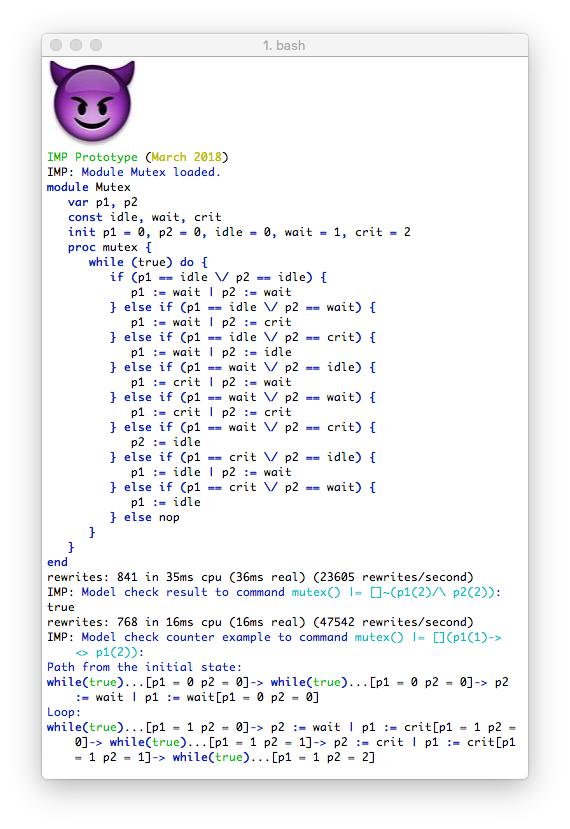
\includegraphics[width=\columnwidth]{imp-mutex.png} \end{center}
%\caption{Loading and model checking a Mutex protocol in \textsc{Imp} that is safe but not live.}
%\label{fig:imp-mutex}
%\end{figure}


\section{Complete IMP compiler in Maude}

\subsection{Parser}

Module {\Tt{}TOKEN\nwendquote} specifies what {\Tt{}Tokens\nwendquote}, {\Tt{}TokenLists\nwendquote} and {\Tt{}NeTokenList\nwendquote} are. They are constructed with operators {\Tt{}token\nwendquote}, {\Tt{}bubble\nwendquote} and {\Tt{}neTokenList\nwendquote}, where attribute {\Tt{}Exclude\nwendquote} specify which terms are not to be constructed by the given constructor.
\nwfilename{imp.noweb}\nwbegincode{1}\moddef{token-module}\endmoddef\nwstartdeflinemarkup\nwenddeflinemarkup
 fmod TOKEN is
 pr QID-LIST .
 sorts Token Bubble TokenList NeTokenList .
 subsort Token < TokenList .

 op _,_ : TokenList TokenList -> TokenList [assoc prec 5] .

 op token : Qid -> Token
    [special
      (id-hook Bubble        (1 1)
       op-hook qidSymbol     (<Qids> : ~> Qid)
       id-hook Exclude       ( true false nop print ))] .

 op bubble : QidList -> Bubble
    [special
      (id-hook Bubble        (1 -1)
       op-hook qidListSymbol (__ : QidList QidList ~> QidList)
       op-hook qidSymbol     (<Qids> : ~> Qid)
       id-hook Exclude       ( | if then else end \{ \} 
                               while ; := = nop )) ] .

 op neTokenList : QidList -> NeTokenList
    [special
      (id-hook Bubble        (1 -1)
       op-hook qidListSymbol (__ : QidList QidList ~> QidList)
       op-hook qidSymbol     (<Qids> : ~> Qid)
       id-hook Exclude       ( . ))] .
endfm
\nwendcode{}\nwbegindocs{2}\nwdocspar

Module {\Tt{}IMP-GRAMMAR\nwendquote} implements the grammar of Section~\ref{sec:imp-grammar} in Maude. Each sort implements a non-terminal of the grammar in Section~\ref{sec:imp-grammar} whereas constants, tokens, as described in module {\Tt{}TOKEN\nwendquote}, or operators implement terminals. For instance, the following rule in the grammar of Section~\ref{sec:imp-grammar}
\begin{grammar}
<proc> := `proc' <ident> `(' <ident>$^*$ `)' <block>
\end{grammar}
is implemented in Module {\Tt{}IMP-GRAMMAR\nwendquote} by the operation declarations
\begin{maude}
 op proc__ : Token BlockCommandDecl -> ProcDecl [prec 50] .
 op proc_`(_`)_ : Token TokenList BlockCommandDecl -> ProcDecl [prec 50] .
\end{maude}
together with the declarations for sorts {\Tt{}ProcDecl\nwendquote} and {\Tt{}BlockCommandDecl\nwendquote}.
\nwenddocs{}\nwbegincode{3}\moddef{imp-grammar-module}\endmoddef\nwstartdeflinemarkup\nwenddeflinemarkup
fmod IMP-GRAMMAR is
 pr TOKEN .
 pr RAT .
 inc PREDICATE-DECL .
 inc COMMAND-DECL .
 sorts VariablesDecl ConstantsDecl OperationsDecl ProcDeclList
       ProcDecl FormalsDecl BlockCommandDecl ExpressionDecl
       InitDecl InitDeclList InitDecls ClausesDecl
       ModuleDecl Expression .

 subsort InitDecl < InitDeclList .
 subsort VariablesDecl ConstantsDecl ProcDeclList 
         InitDecls < ClausesDecl .
 subsort BlockCommandDecl < CommandDecl .
 subsort ProcDecl < ProcDeclList .
 subsort PredicateDecl < ExpressionDecl .

 *** Boolean expressions
 op _==_ : Token Token -> PredicateDecl [prec 30] .
 op _==_ : Token ExpressionDecl -> PredicateDecl [prec 30] .
 op _==_ : ExpressionDecl Token -> PredicateDecl [prec 30] .
 op _==_ : ExpressionDecl ExpressionDecl -> PredicateDecl 
           [prec 30] .
 op _/\\_ : PredicateDecl PredicateDecl -> PredicateDecl 
           [assoc comm prec 35] .
 op ~ : PredicateDecl -> PredicateDecl .

 *** Arithmetic expressions
 op _+_ : Token Token -> ExpressionDecl [gather(e E) prec 15] .
 op _+_ : Token ExpressionDecl -> ExpressionDecl [gather(e E) prec 15] .
 op _+_ : ExpressionDecl Token -> ExpressionDecl [gather(e E) prec 15] .
 op _+_ : ExpressionDecl ExpressionDecl -> ExpressionDecl 
          [gather(e E) prec 15] .

 op _-_ : Token Token -> ExpressionDecl  [gather(e E) prec 15] .
 op _-_ : Token ExpressionDecl -> ExpressionDecl [gather(e E) prec 15] .
 op _-_ : ExpressionDecl Token -> ExpressionDecl [gather(e E) prec 15] .
 op _-_ : ExpressionDecl ExpressionDecl -> ExpressionDecl 
          [gather(e E) prec 15] .

 op _*_ : Token Token -> ExpressionDecl [gather(e E) prec 10] .
 op _*_ : Token ExpressionDecl -> ExpressionDecl [gather(e E) prec 10] .
 op _*_ : ExpressionDecl Token -> ExpressionDecl [gather(e E) prec 10] .
 op _*_ : ExpressionDecl ExpressionDecl -> ExpressionDecl 
          [gather(e E) prec 10] .

 op _/_ : Token Token -> ExpressionDecl [prec 20] .
 op _/_ : Token ExpressionDecl -> ExpressionDecl [prec 20] .
 op _/_ : ExpressionDecl Token -> ExpressionDecl [prec 20] .
 op _/_ : ExpressionDecl ExpressionDecl -> ExpressionDecl [prec 20] .

 *** Commands
 op _:=_ : Token Token -> CommandDecl [prec 40] .
 op _:=_ : Token ExpressionDecl -> CommandDecl [prec 40] .

 op _() : Token -> CommandDecl .
 op _(_) : Token Bubble -> CommandDecl .
 op print : Token -> CommandDecl .
 op print : ExpressionDecl -> CommandDecl .
 op _;_ : CommandDecl CommandDecl -> CommandDecl [assoc prec 50] .
 op _|_ : CommandDecl CommandDecl -> CommandDecl [assoc prec 50] .
 op while_do_ : PredicateDecl BlockCommandDecl -> CommandDecl [prec 40] .
 op \{_\} : CommandDecl -> BlockCommandDecl [prec 35] .
 op if__else_ : PredicateDecl CommandDecl CommandDecl -> CommandDecl 
    [prec 40] .

 *** Declarations
 op module__end : Token ClausesDecl -> ModuleDecl [prec 80] .
 op __ : ClausesDecl ClausesDecl -> ClausesDecl [assoc comm prec 70] .
 op var_ : TokenList -> VariablesDecl [prec 60] .
 op const_ : TokenList -> ConstantsDecl [prec 60] .
 op init_ : InitDecl -> InitDecls [prec 60] .
 op init_ : InitDeclList -> InitDecls  [prec 60] .
 op _=_ : Token Token -> InitDecl  [prec 40] .
 op _=_ : Token ExpressionDecl -> InitDecl  [prec 40] .
 op _,_ : InitDeclList InitDeclList -> InitDeclList  [assoc prec 50] .
 op proc__ : Token BlockCommandDecl -> ProcDecl [prec 50] .
 op proc_`(_`)_ : Token TokenList BlockCommandDecl -> ProcDecl  
    [prec 50] .
 op __ : ProcDeclList ProcDeclList -> ProcDeclList  
   [assoc comm prec 60] .
endfm 
\nwendcode{}\nwbegindocs{4}\nwdocspar

\subsection{Compiling to $\uppi$ lib}

Compilation from IMP to $\uppi$ lib is quite trivial as there exists a one-to-one correspondence between IMP constructions and $\uppi$ lib basic programming language constructs. Essentially, an IMP {\Tt{}module\nwendquote} gives rise to a $\uppi$ {\Tt{}dec\nwendquote}. IMP {\Tt{}var\nwendquote} and {\Tt{}const\nwendquote} are declarations and so is a {\Tt{}proc\nwendquote} declaration that gives rise to a {\Tt{}prc\nwendquote} declaration in $\uppi$. 
\nwenddocs{}\nwbegincode{5}\moddef{compile-imp-to-bplc}\endmoddef\nwstartdeflinemarkup\nwenddeflinemarkup
mod COMPILE-IMP-TO-BPLC is
 inc PREDICATE-DECL .
 inc COMMAND-DECL .
 pr BPLC .
 pr META-LEVEL .

 \LA{}Compiling IMP expressions to BPLC Exp\RA{}
 \LA{}Compiling IMP commands to BPLC Cmd\RA{} 
 \LA{}Compiling IMP declarations to BPLC Dec\RA{}
\nwendcode{}\nwbegindocs{6}\nwdocspar

The compilation from IMP to $\uppi$ exp relates IMP tokens to $\uppi$ Id, IMP arithmetic and boolean expressions to $\uppi$ Exp. In particular, the compilation of a {\Tt{}token\nwendquote} has to check if the token is a primitive type, either {\Tt{}Rat\nwendquote} (for Rational numbers) or {\Tt{}Bool\nwendquote} (for Boolean values), or an identifier. Since {\Tt{}Rat\nwendquote} and {\Tt{}Bool\nwendquote} are tokenized and we need Maude metalevel descent function {\Tt{}downTerm\nwendquote} to help us parse them into proper constants
 
\nwenddocs{}\nwbegincode{7}\moddef{Compiling tokens}\endmoddef\nwstartdeflinemarkup\nwenddeflinemarkup
 op compileId : Qid -> Id .
 eq compileId(I:Qid) = idn(downTerm(I:Qid, 'Qid)) .

 op compileId : Term -> Id .
 eq compileId('token[I:Qid]) =
    if (metaParse(upModule('RAT, false), 
         downTerm(I:Qid, 'Qid), 'Rat)  :: ResultPair)
        then rat(downTerm(getTerm(metaParse(upModule('RAT, false),
              downTerm(I:Qid, 'Qid), 'Rat)), 1/2))
    else
     if (metaParse(upModule('BOOL, false), 
          downTerm(I:Qid, 'Qid), 'Bool) :: ResultPair)
     then boo(downTerm(getTerm(metaParse(upModule('BOOL, false),
                   downTerm(I:Qid, 'Qid), 'Bool)), true))
     else idn(downTerm(I:Qid, 'Qid))
     fi
    fi .
\nwendcode{}\nwbegindocs{8}\nwdocspar

Arithmetic expressions are mapped to their prefixed counterpart in $\uppi$, e.g, an IMP expression {\Tt{}a\ +\ b\nwendquote} is compiled to {\Tt{}add(compileExp(a),\ compileExp(b))\nwendquote}.
\nwenddocs{}\nwbegincode{9}\moddef{Compiling arithmetic expressions}\endmoddef\nwstartdeflinemarkup\nwenddeflinemarkup
 op compileExp : Term -> Exp .
 ceq compileExp(I:Qid) = compileId(I:Qid) 
  if not(I:Qid :: Constant) .
 eq compileExp('token[I:Qid]) = compileId('token[I:Qid]) .
 eq compileExp('_+_[T1:Term, T2:Term]) =
     add(compileExp(T1:Term), compileExp(T2:Term)) .
 eq compileExp('_-_[T1:Term, T2:Term]) =
     sub(compileExp(T1:Term), compileExp(T2:Term)) .
 eq compileExp('_*_[T1:Term, T2:Term]) =
     mul(compileExp(T1:Term), compileExp(T2:Term)) .
 eq compileExp('_/_[T1:Term, T2:Term]) =
     div(compileExp(T1:Term), compileExp(T2:Term)) .
\nwendcode{}\nwbegindocs{10}\nwdocspar

A treatment similar to arithmetic expressions is given to Boolean expressions, with a particular care with constants, as we did in  <<Compiling tokens>>. Here, however, we do not require a call to {\Tt{}downTerm\nwendquote} as the constants for {\Tt{}PredicateDecl\nwendquote} are already typed.
\nwenddocs{}\nwbegincode{11}\moddef{Compiling boolean expressions}\endmoddef\nwstartdeflinemarkup\nwenddeflinemarkup
 eq compileExp('true.PredicateDecl) = boo(true) .
 eq compileExp('false.PredicateDecl) = boo(false) .
 eq compileExp('~[T:Term]) = neg(compileExp(T:Term)) .
 eq compileExp('_/\\_[T1:Term,T2:Term]) = 
    and(compileExp(T1:Term), compileExp(T2:Term)) .
 eq compileExp('_\\/_[T1:Term,T2:Term]) = 
    or(compileExp(T1:Term), compileExp(T2:Term)) .
 eq compileExp('_==_[T1:Term,T2:Term]) = 
    eq(compileExp(T1:Term), compileExp(T2:Term)) .
 eq compileExp('_>_[T1:Term,T2:Term]) = 
    gt(compileExp(T1:Term), compileExp(T2:Term)) .
 eq compileExp('_>=_[T1:Term,T2:Term]) = 
    ge(compileExp(T1:Term), compileExp(T2:Term)) .
 eq compileExp('_<_[T1:Term,T2:Term]) =  
    lt(compileExp(T1:Term), compileExp(T2:Term)) .
 eq compileExp('_<=_[T1:Term,T2:Term]) = 
    le(compileExp(T1:Term), compileExp(T2:Term)) .
\nwendcode{}\nwbegindocs{12}\nwdocspar

\nwenddocs{}\nwbegincode{13}\moddef{Compiling IMP commands to BPLC Cmd}\endmoddef\nwstartdeflinemarkup\nwenddeflinemarkup
 op compileCmd : Term -> Cmd .
 eq compileCmd('nop.CommandDecl) = nop .
 eq compileCmd('_:=_['token[I:Qid], T:Term]) =
    assign(compileId('token[I:Qid]), compileExp(T:Term)) .
 eq compileCmd('`\{_`\}[T:Term]) = blk(compileCmd(T:Term)) .
 eq compileCmd('_;_[T1:Term, T2:Term]) =
    seq(compileCmd(T1:Term), compileCmd(T2:Term)) .
 eq compileCmd('_|_[T1:Term, T2:Term]) =
    choice(compileCmd(T1:Term), compileCmd(T2:Term)) .
 eq compileCmd('if__else_[T1:Term, T2:Term, T3:Term]) =
    if(compileExp(T1:Term), compileCmd(T2:Term), 
       compileCmd(T3:Term)) .
 eq compileCmd('while_do_[T1:Term, T2:Term]) =
    loop(compileExp(T1:Term), compileCmd(T2:Term)) .
 eq compileCmd('print[T:Term]) = print(compileId(T:Term)) .

 *** Compiling IMP commands to BPLC Cmd:
 *** Procedure calls deserve more attention...

 eq compileCmd('_`(`)['token[I:Qid]]) =
    cal(compileId('token[I:Qid])) .
 eq compileCmd('_`(_`)['token[I:Qid], 'bubble[Q:Qid]]) =
    cal(compileId('token[I:Qid]), compileActuals(Q:Qid)) .
 eq compileCmd('_`(_`)['token[I:Qid], 
               'bubble['__[TL:TermList]]]) =
    cal(compileId('token[I:Qid]), compileActuals(TL:TermList)) .

 op compileActuals : TermList -> Actuals .
 eq compileActuals(Q:Qid) = compileId('token[Q:Qid]) .
 eq compileActuals((TL1:TermList, ''`,.Qid , TL2:TermList)) =
    act(makeExp(TL1:TermList) , compileActuals(TL2:TermList)) .
 eq compileActuals(TL:TermList) = makeExp(TL:TermList) [owise] .
 
 op makeExp : TermList -> Exp .
 eq makeExp(Q:Qid) = compileId(Q:Qid) .
 ceq makeExp(TL:TermList) =
     compileExp(
      getTerm(
       metaParse(upModule('IMP-GRAMMAR, false),
        makeExprDeclQidList(TL:TermList), 'ExpressionDecl)))
  if (metaParse(upModule('IMP-GRAMMAR, false),
             makeExprDeclQidList(TL:TermList), 'ExpressionDecl) ::
            ResultPair) .

 op makeExprDeclQidList : TermList -> QidList .
 eq makeExprDeclQidList((empty).TermList) = (nil).QidList .
 ceq makeExprDeclQidList(Q:Qid) = downTerm(Q:Qid, 'error)
  if downTerm(Q:Qid, 'error) =/= 'error .
 eq makeExprDeclQidList((Q:Qid , TL:TermList)) =
    makeExprDeclQidList(Q:Qid) makeExprDeclQidList(TL:TermList) .
\nwendcode{}\nwbegindocs{14}\nwdocspar

\nwenddocs{}\nwbegincode{15}\moddef{Compiling IMP declarations to BPLC Dec}\endmoddef\nwstartdeflinemarkup\nwenddeflinemarkup
 *** Compiling variables. The initialization clause is 
 *** necessary to properly declare variables according to BPLC 
 *** ref construct.

 op compileVar : Term Term -> Dec .
 op $compileVar : Term Term -> Dec .
 eq compileVar('var_[TL1:TermList], 'init_[TL2:TermList]) =
    $compileVar(TL1:TermList, TL2:TermList) .
 eq $compileVar('token[I:Qid], '_=_['token[I:Qid], T:Term]) =
    ref(compileId('token[I:Qid]), compileExp(T:Term)) .
 eq $compileVar('token[I:Qid], 
    ('_`,_['_=_['token[I:Qid], T:Term], TL:TermList])) =
    ref(compileId('token[I:Qid]), compileExp(T:Term)) .
 ceq $compileVar('token[I1:Qid], 
     ('_`,_['_=_['token[I2:Qid], T:Term], TL:TermList])) =
     $compileVar('token[I1:Qid], TL:TermList)
  if I1:Qid =/= I2:Qid .
 eq $compileVar('_`,_['token[I:Qid], IS:TermList], 
                 '_=_['token[I:Qid], T:Term]) =
    ref(compileId('token[I:Qid]), compileExp(T:Term)) .
 eq $compileVar('_`,_['token[I:Qid], IS:TermList], 
                '_`,_[TL:TermList]) =
    dec($compileVar('token[I:Qid], '_`,_[TL:TermList]),
     $compileVar(IS:TermList, '_`,_[TL:TermList])) .

 *** Compiling constants.
 op compileConst : Term Term -> Dec .
 op $compileConst : Term Term -> Dec .
 eq compileConst('const_[T1:Term], 'init_[T2:Term]) =
    $compileConst(T1:Term, T2:Term) .
 eq $compileConst('token[I:Qid], 
                  '_=_['token[I:Qid], T:Term]) =
    cns(compileId('token[I:Qid]), compileExp(T:Term)) .
 eq $compileConst('token[I:Qid], 
                 ('_`,_['_=_['token[I:Qid], T:Term], TL:TermList])) =
    cns(compileId('token[I:Qid]), compileExp(T:Term)) .
ceq $compileConst('token[I1:Qid], 
                 ('_`,_['_=_['token[I2:Qid], T:Term], TL:TermList])) =
    $compileConst('token[I1:Qid], TL:TermList)
 if I1:Qid =/= I2:Qid .
 eq $compileConst('_`,_['token[I:Qid], IS:TermList], 
                  '_=_['token[I:Qid], T:Term]) =
    cns(compileId('token[I:Qid]), compileExp(T:Term)) .
 eq $compileConst('_`,_['token[I:Qid], IS:TermList], '_`,_[TL:TermList]) =
    dec($compileConst('token[I:Qid], '_`,_[TL:TermList]),
     $compileConst(IS:TermList, '_`,_[TL:TermList])) .

 *** Compiling procedure declarations.
 op compileProc : TermList -> Dec .
 op compileToFormals : TermList -> Formals .
 eq compileProc('__[TL1:TermList, TL2:TermList]) =
    dec(compileProc(TL1:TermList), compileProc(TL2:TermList)) .
 eq compileProc('proc__['token[O:Qid], TL:TermList, T:Term]) =
    prc(compileId('token[O:Qid]), compileCmd(T:Term)) .
 eq compileProc('proc_`(_`)_['token[O:Qid], TL:TermList, T:Term]) =
    prc(compileId('token[O:Qid]),
     compileToFormals(TL:TermList), compileCmd(T:Term)) .
 eq compileToFormals('token[O:Qid]) = par(compileId('token[O:Qid])) .
 eq compileToFormals('_`,_[TL1:TermList, TL2:TermList]) =
    for(compileToFormals(TL1:TermList), compileToFormals(TL2:TermList)) .

 *** Compiling modules.
 op compileMod : Term -> Dec .
 eq compileMod('module__end['token[I:Qid],
               '__['var_[T1:Term],
               '__['const_[T2:Term],
               '__['init_[T3:Term],
                                T:Term]]]]) =
    dec(compileVar('var_[T1:Term],'init_[T3:Term]),
     dec(compileConst('const_[T2:Term], 'init_[T3:Term]),
      compileProc(T:Term))) .
 eq compileMod('module__end['token[I:Qid],
               '__['var_[T1:Term],
               '__['init_[T3:Term],
               T:Term]]]) =
    dec(compileVar('var_[T1:Term],'init_[T3:Term]),
         compileProc(T:Term)) .
 eq compileMod('module__end['token[I:Qid],
               '__['var_[T1:Term],
               '__['const_[T2:Term],
               '__['init_[T3:Term],
               '__[TL:TermList]]]]]) =
    dec(compileVar('var_[T1:Term],'init_[T3:Term]),
     dec(compileConst('const_[T2:Term], 'init_[T3:Term]),
          compileProc('__[TL:TermList]))) .
 eq compileMod('module__end['token[I:Qid],
               '__['var_[T1:Term],
               '__['init_[T3:Term],
               '__[TL:TermList]]]]) =
    dec(compileVar('var_[T1:Term],'init_[T3:Term]),
         compileProc('__[TL:TermList])) .
endm
\nwendcode{}\nwbegindocs{16}\nwdocspar

\subsection{Pretty-printing IMP programs, their execution and model checking results}

\nwenddocs{}\nwbegincode{17}\moddef{imp-pretty-printing}\endmoddef\nwstartdeflinemarkup\nwenddeflinemarkup
mod IMP-PRETTY-PRINTING is
 pr BPLC-MODEL-CHECKER .
 pr COMPILE-TO-PYTHON . 
 pr INT .

 op printTermList : TermList -> QidList .
 eq printTermList(empty) = (nil).QidList .
 eq printTermList((Q:Qid,TL:TermList)) =
    downTerm(Q:Qid,'Qid) printTermList(TL:TermList) .

 op printTokens : Term -> QidList .
 eq printTokens(Q:Qid) = Q:Qid .
 eq printTokens('token[Q:Qid]) = downTerm(Q:Qid, 'Qid) .
 eq printTokens('_`,_[T1:Term, T2:Term]) =
    printTokens(T1:Term) printToken('`,) '\\s printTokens(T2:Term) .

 *** Pretty-printing IMP Expressions
 op printExp : Term -> QidList .
 eq printExp('true.PredicateDecl) = 'true .
 eq printExp('false.PredicateDecl) = 'false .
 eq printExp('bubble['__[TL:TermList]]) = printTermList(TL:TermList) .
 eq printExp('token[Q:Qid]) = downTerm(Q:Qid, 'Qid) .
 eq printExp('_==_[T1:Term, T2:Term]) =
    printExp(T1:Term) printToken('==) printExp(T2:Term) .
 eq printExp('_\\/_[T1:Term, T2:Term]) =
    printExp(T1:Term) printToken('\\/) printExp(T2:Term) .
 eq printExp('_/\\_[T1:Term, T2:Term]) =
    printExp(T1:Term) printToken('\\/) printExp(T2:Term) .
 eq printExp('~[T:Term]) =
    printToken('~) printExp(T:Term) .
 eq printExp('_<_[T1:Term, T2:Term]) =
    printExp(T1:Term) printToken('<) printExp(T2:Term) .
 eq printExp('_<=_[T1:Term, T2:Term]) =
    printExp(T1:Term) printToken('<=) printExp(T2:Term) .
 eq printExp('_>_[T1:Term, T2:Term]) =
    printExp(T1:Term) printToken('>) printExp(T2:Term) .
 eq printExp('_>=_[T1:Term, T2:Term]) =
    printExp(T1:Term) printToken('>=) printExp(T2:Term) .
 eq printExp('_+_[T1:Term, T2:Term]) =
    printExp(T1:Term) printToken('+) printExp(T2:Term) .
 eq printExp('_*_[T1:Term, T2:Term]) =
    printExp(T1:Term) printToken('*) printExp(T2:Term) .
 eq printExp('_-_[T1:Term, T2:Term]) =
    printExp(T1:Term) printToken('-) printExp(T2:Term) .
 eq printExp('_/_[T1:Term, T2:Term]) =
    printExp(T1:Term) printToken('/) printExp(T2:Term) .
 eq printExp(T:Term) =
    metaPrettyPrint(upModule('IMP-GRAMMAR, false), T:Term) [owise] .

 *** Pretty-printing IMP Commands
 op printCmd : Term Nat -> QidList .
 eq printCmd('nop.CommandDecl, N:Nat) = 'nop .
 eq printCmd('print[T:Term], N:Nat) =
    printToken('print) printToken('`() printExp(T:Term) printToken('`)) .
 eq printCmd('_`(_`)[T1:Term, T2:Term], N:Nat) =
    printExp(T1:Term) printToken('`() printExp(T2:Term) printToken('`)) .
 eq printCmd('_|_[T1:Term, '_;_[T2:TermList]], N:Nat) =
    printSpaces(N:Nat)
    printCmd(T1:Term, N:Nat) printToken('|) '\\n
    printSpaces(N:Nat) printToken('`() 
    printCmd('_;_[T2:TermList], N:Nat) printToken('`)) .
ceq printCmd('_|_[T:TermList, F:Qid[TL:TermList]], N:Nat) =
    printSpaces(N:Nat) printCmd(T:TermList, N:Nat) printToken('|)
    printCmd(F:Qid[TL:TermList], N:Nat)
 if F:Qid =/= '_;_ .
ceq printCmd('_;_[F1:Qid[TL1:TermList], F2:Qid[TL2:TermList]], N:Nat) =
    printCmd(F1:Qid[TL1:TermList], N:Nat) '\\s printToken(';)
    printCmd(F2:Qid[TL2:TermList], N:Nat)
 if F1:Qid =/= '_;_ and F2:Qid =/= '_;_ .
ceq printCmd('_;_[F1:Qid[TL1:TermList], F2:Qid[TL2:TermList]], N:Nat) =
    printSpaces(N:Nat) 
    printCmd(F1:Qid[TL1:TermList], N:Nat) '\\s printToken(';) '\\n
    printSpaces(N:Nat) 
    printCmd(F1:Qid[TL1:TermList], N:Nat)
 if F1:Qid == '_;_ or F2:Qid == '_;_ .
 eq printCmd('_:=_[T1:Term, T2:Term], N:Nat) =
    printExp(T1:Term) printToken(':=) printExp(T2:Term) .
 eq printCmd('while_do_[T1:Term, T2:Term], N:Nat) =
    printToken('while) ' printToken('`() printExp(T1:Term) printToken('`)) '
    printToken('do)
    printCmd(T2:Term, N:Nat) .
 eq printCmd('if__else_[T1:Term, T2:Term, T3:Term], N:Nat) =
    printToken('if) ' printToken('`() printExp(T1:Term) printToken('`)) '
    printCmd(T2:Term, N:Nat)
    '\\s printToken('else) printCmd(T3:Term, N:Nat) .
 eq printCmd('`\{_`\}[C:Constant], N:Nat) =
    '\\s printToken('`\{) 
    printCmd(C:Constant, 0) 
    printToken('`\}) .
 eq printCmd('`\{_`\}['_;_[TL:TermList]], N:Nat) =
    '\\s printToken('`\{) '\\n
    printSpaces(N:Nat + incr) 
    printCmd('_;_[TL:TermList], N:Nat + incr) '\\n
    printSpaces(N:Nat) printToken('`\}) .
 eq printCmd('`\{_`\}['_|_[TL:TermList]], N:Nat) =
    '\\s printToken('`\{) '\\n 
    printCmd('_|_[TL:TermList], N:Nat + incr) '\\n
    printSpaces(N:Nat) printToken('`\}) .
ceq printCmd('`\{_`\}[F:Qid[TL:TermList]], N:Nat) =
    '\\s printToken('`\{) '\\n
    printSpaces(N:Nat + incr) 
    printCmd(F:Qid[TL:TermList], N:Nat + incr) '\\n
    printSpaces(N:Nat) printToken('`\})
 if F:Qid =/= '_;_ /\\ F:Qid =/= '_|_ .

 eq printCmd(T:Term, N:Nat) =
    printSpaces(N:Nat) 
    metaPrettyPrint(upModule('IMP-GRAMMAR, false), T:Term) [owise] .

 *** Pretty-printing IMP Declarations
 op printModule : Term -> QidList .
 eq printModule('module__end[T1:Term, T2:Term]) =
    printToken('module) printTokens(T1:Term)
        printClauses(T2:Term)
        '\\n printToken('end) .

 op printClauses : Term -> QidList .
 eq printClauses('proc__[T1:Term, T2:Term]) =
    '\\n printSpaces(level)
    printToken('proc) printTokens(T1:Term)
    printCmd(T2:Term, level) .
 eq printClauses('__['proc__[T1:Term, T2:Term], T3:Term]) =
    '\\n printSpaces(level) printToken('proc) printTokens(T1:Term)
    printCmd(T2:Term, level)
    printClauses(T3:Term) .
 eq printClauses('proc_`(_`)_[T1:Term, T2:Term, T3:Term]) =
    '\\n printSpaces(level)
    printToken('proc) printTokens(T1:Term)
    printToken('`() printTokens(T2:Term) printToken('`))
    printCmd(T3:Term, level) .
 eq printClauses('__['proc_`(_`)_[T1:Term, T2:Term, T3:Term], T4:Term]) =
    '\\n printSpaces(level) printToken('proc) 
    printTokens(T1:Term) printToken('`() printTokens(T2:Term) printToken('`)) 
    printCmd(T3:Term, level)
    printClauses(T4:Term) .
 eq printClauses('__['init_[T1:Term], T2:Term]) =
    '\\n printSpaces(level) printToken('init) 
    printInit(T1:Term) printClauses(T2:Term) .
 eq printClauses('__['const_[T1:Term], T2:Term]) =
    '\\n printSpaces(level) printToken('const) 
    printTokens(T1:Term) printClauses(T2:Term) .
 eq printClauses('__['var_[T1:Term], T2:Term]) =
        '\\n printSpaces(level) printToken('var) 
    printTokens(T1:Term) printClauses(T2:Term) .
 
 op printInit : Term -> QidList .
 eq printInit('_=_[T1:Term, T2:Term]) =
    printTokens(T1:Term) printToken('=) printExp(T2:Term) .
 eq printInit('_`,_[T1:Term, T2:Term]) =
    printInit(T1:Term) printToken('`,) '\\s printInit(T2:Term) .

 *** Pretty-printing parse error
 op printQidList : QidList -> QidList .
 eq printQidList(nil) = (nil).QidList .
 eq printQidList(Q:Qid QL:QidList) = printToken(Q:Qid) printQidList(QL:QidList) .

 op printToken : Qid -> Qid .
 eq printToken(Q:Qid) = '\\b '\\! Q:Qid '\\o .

 op printInputWithError : QidList Nat -> QidList .
 op $printInputWithError : QidList Int QidList -> QidList .
 eq printInputWithError(QL:QidList, N:Nat) =
    $printInputWithError(QL:QidList, N:Nat, (nil).QidList) .
 eq $printInputWithError(nil, I:Int, QL:QidList) = QL:QidList .
 eq $printInputWithError(QL:QidList, 0, (nil).QidList) = (nil).QidList .
ceq $printInputWithError(QL1:QidList, 0, (QL2:QidList Q:Qid)) =
    QL2:QidList '\\r '\\u '>>> Q:Qid '<<< 'HERE '\\o
    printQidList(QL1:QidList)
 if QL2:QidList =/= nil .
 eq $printInputWithError(Q:Qid QL1:QidList, I:Int, QL2:QidList) =
    $printInputWithError(QL1:QidList, (I:Int + (- 1)), QL2:QidList
        printToken(Q:Qid)) .

 op printParseError : QidList ResultPair? -> Qid .
 eq printParseError('module Q:Qid QL:QidList , noParse(N:Nat)) =
    'IMP: 'Error 'at 'position
    metaPrettyPrint(upModule('NAT, false), upTerm(N:Nat))
        'while 'parsing 'Module Q:Qid ': '\\n
        printInputWithError(('module Q:Qid QL:QidList), N:Nat) .
 eq printParseError(QL:QidList, ambiguity(T1:ResultPair, T2:ResultPair)) =
    'IMP: '\\r 'Ambiguous 'parse '\\o '\\n
    metaPrettyPrint(upModule('IMP-GRAMMAR, false), getTerm(T1:ResultPair)) '\\n
    '\\r 'vs. '\\o '\\n
    metaPrettyPrint(upModule('IMP-GRAMMAR, false), getTerm(T2:ResultPair)) .

 *** Pretty-print exec and mc output
 op printState : Env Store -> QidList .
 eq printState(noEnv, S:Store) = (nil).QidList .
 eq printState((I:Id |-> bind(L:Loc)) , ((L:Loc |-> store(R:Rat)), S:Store)) =
    printId(I:Id) '= metaPrettyPrint(upModule('RAT, false), upTerm(R:Rat)) .
ceq printState(((I:Id |-> bind(L:Loc)), E:Env) ,
    ((L:Loc |-> store(R:Rat)), S:Store)) =
    printId(I:Id) '=
    metaPrettyPrint(upModule('RAT, false), upTerm(R:Rat))
    printState(E:Env , (L:Loc |-> store(R:Rat), S:Store))
 if E:Env =/= noEnv .
 eq printState((I:Id |-> bind(L:Loc)), (L:Loc |-> store(B:Bool), S:Store)) =
    printId(I:Id) '= metaPrettyPrint(upModule('BOOL, false), upTerm(B:Bool)) .
ceq printState(((I:Id |-> bind(L:Loc)), E:Env) ,
    ((L:Loc |-> store(B:Bool)), S:Store)) =
        printId(I:Id) '= metaPrettyPrint(upModule('RAT, false), upTerm(B:Bool)) '`,
        printState(E:Env , (L:Loc |-> store(B:Bool), S:Store))
 if E:Env =/= noEnv .
 eq printState(((I:Id |-> B:Bindable), E:Env) , S:Store) =
    printState(E:Env , S:Store) [owise] .

 op printId : Id -> Qid .
 eq printId(idn(Q:Qid)) = (Q:Qid).Qid .
 
 op printCnt : ControlStack ValueStack -> QidList .
 eq printCnt((LOOP C:ControlStack), 
             (V:Value val(loop(E:Exp, K:Cmd)) VS:ValueStack)) =
    printToken('while) printToken('`() printExp(E:Exp) printToken('`)) '... .
 eq printCnt((choice(K1:Cmd, K2:Cmd) C:ControlStack), VS:ValueStack) =
    printCmd(K1:Cmd) printToken('|) printCmd(K2:Cmd) .
 eq printCnt(C:ControlStack, VS:ValueStack) =
    '\\n 'Constrol 'stack:
    metaPrettyPrint(upModule('BPLC+META-LEVEL, false),
     upTerm(C:ControlStack))
    '\\n 'Value 'stack:
     metaPrettyPrint(upModule('BPLC+META-LEVEL, false),
     upTerm(VS:ValueStack)) .

 op printExp : Exp -> QidList .
 eq printExp(rat(R:Rat)) = '\\g metaPrettyPrint(upModule('RAT, false),
     upTerm(R:Rat)) '\\o .
 eq printExp(boo(B:Bool)) = '\\g metaPrettyPrint(upModule('BOOL, false),
     upTerm(B:Bool)) '\\o .
 eq printExp(neg(E:Exp)) = printToken('~) printExp(E:Exp) .
 eq printExp(and(E1:Exp, E2:Exp)) = 
    printExp(E1:Exp) printToken('/\\) printExp(E2:Exp) .
 eq printExp(eq(E1:Exp, E2:Exp)) = 
    printExp(E1:Exp) printToken('==) printExp(E2:Exp) .
 eq printExp(idn(Q:Qid)) = printTokens(Q:Qid) .
 eq printExp(E:Exp) = metaPrettyPrint(upModule('BPLC, false), upTerm(E:Exp)) .

 op printCmd : Cmd -> QidList .
 eq printCmd(seq(C1:Cmd, C2:Cmd)) = 
    printCmd(C1:Cmd) printToken(';) printCmd(C2:Cmd) .
 eq printCmd(assign(I:Id, E:Exp)) = 
    printExp(I:Id) printToken(':=) printExp(E:Exp) .
 eq printCmd(if(E:Exp, C1:Cmd, C2:Cmd)) = 
    printToken('if) printExp(E:Exp) '... .
 eq printCmd(choice(C1:Cmd, C2:Cmd)) = printCmd(C1:Cmd)
    printToken('|) printCmd(C2:Cmd) .
 eq printCmd(C:Cmd) = metaPrettyPrint(upModule('BPLC, false), upTerm(C:Cmd)) .

 op printConf : Conf -> QidList .
 eq printConf(< env : E:Env , sto : S:Store , exc : X:Exc , 
                cnt : C:ControlStack, val : V:ValueStack, ...:Set\{SemComp\} > ) =
    if X:Exc == CNT
    then printCnt(C:ControlStack, V:ValueStack) '`[ printState(E:Env, S:Store) '`]
        else 'IMP: 'Internal 'error 'while 'printing 'configuration.  
    fi .

 op printValueStack : ValueStack -> QidList .
 eq printValueStack(evs) = '\\b 'No 'output. '\\o .
 eq printValueStack(val(R:Rat) evs) =
    metaPrettyPrint(upModule('RAT, false), upTerm(R:Rat)) .
 eq printValueStack(val(B:Bool) evs) =
    metaPrettyPrint(upModule('BOOL, false), upTerm(B:Bool)) .
 eq printValueStack(V:Value VS:ValueStack) =
    printValueStack(V:Value) printValueStack(VS:ValueStack) .
 
 op printOut : Conf -> QidList .
 eq printOut(< out : O:ValueStack , ...:Set\{SemComp\} > ) =
    printValueStack(O:ValueStack) .

 op printExec : Term ~> QidList .
ceq printExec(T:Term) = printOut(downTerm(T:Term, < noSemComp >))
 if downTerm(T:Term, < noSemComp >) =/= < noSemComp > .

 op printTraceStep : TraceStep -> QidList .
 eq printTraceStep(\{T:Term, Y:Type, R:Rule\}) =
    printConf(downTerm(T:Term, < noSemComp >)) .

 op printTrace : Trace Nat -> QidList .
 eq printTrace(nil, N:Nat) = (nil).QidList .
 eq printTrace(TS:TraceStep, N:Nat) =
    '\\b 'State 
    metaPrettyPrint(upModule('NAT, false), 
     upTerm(N:Nat)) ': '\\o '\\n
    printTraceStep(TS:TraceStep) .
ceq printTrace(TS:TraceStep T:Trace, N:Nat) =
    '\\b 'State 
    metaPrettyPrint(upModule('NAT, false), 
     upTerm(N:Nat)) ': '\\o '\\n
    printTraceStep(TS:TraceStep) '\\n printTrace(T:Trace, (N:Nat + 1))
 if T:Trace =/= nil .

 op printTransitionList : TransitionList -> QidList .
 eq printTransitionList(nil) = (nil).QidList .
 eq printTransitionList(\{C:Conf, R:RuleName\}) = printConf(C:Conf) .
ceq printTransitionList(\{C:Conf, R:RuleName\} TL:TransitionList) =
    printConf(C:Conf) '\\b '-> '\\o printTransitionList(TL:TransitionList)
 if TL:TransitionList =/= nil .

 op printModelCheckResult : ModelCheckResult QidList -> QidList .
 eq printModelCheckResult(B:Bool, QL:QidList) =
    'IMP: '\\b 'Model 'check 'result 'to 'command 
    '\\c QL:QidList '\\o '\\b ': '\\o '\\n
        metaPrettyPrint(upModule('BOOL, false), upTerm(B:Bool)) .

 eq printModelCheckResult(
    counterexample(TL1:TransitionList, TL2:TransitionList), QL:QidList) =
    'IMP: '\\b 'Model 'check 'counter 'example 'to 'command 
    '\\c QL:QidList '\\o '\\b ': '\\o '\\n
    '\\b 'Path 'from 'the 'initial 'state: '\\o
    '\\n printTransitionList(TL1:TransitionList)
    '\\n '\\b 'Loop: '\\o
    '\\n printTransitionList(TL2:TransitionList) .
endm
\nwendcode{}\nwbegindocs{18}\nwdocspar

\subsection{IMP command line interface}

\nwenddocs{}\nwbegincode{19}\moddef{imp-interface}\endmoddef\nwstartdeflinemarkup\nwenddeflinemarkup
mod IMP-INTERFACE is
 pr LOOP-MODE * (sort State to LoopState).
 pr COMPILE-IMP-TO-BPLC .
 pr IMP-PRETTY-PRINTING .

 sorts Dec? MetaIMPModule Command IMPState .
 subsort Term < MetaIMPModule .
 subsort Dec < Dec? .
 subsort IMPState < LoopState .

 op noDec : -> Dec? .
 op noModule : -> MetaIMPModule .
 op idle : -> Command .
 op <_;_;_> : MetaIMPModule Dec? QidList -> IMPState .
 op init : -> System .
 op init`IMP`no`banner : -> System .
 op banner : -> QidList .
 
 eq banner = '\\g 'IMP 'Prototype '\\o ' 
             '`( '\\y '\\! 'March '2018 '\\o '`) .
 eq init = [nil, < noModule ; noDec ; nil >, banner] .
 eq init`IMP`no`banner = [nil, < noModule ; noDec ; nil >, nil] .

 vars QIL QIL' QIL'' QIL1 QIL2 : QidList .

 rl [version] : ['version, L:LoopState, QIL] => 
                [nil, L:LoopState, banner] .

 *** Loading a module.
 crl [in] : ['module Q:Qid QIL, 
             < M:MetaIMPModule ; D:Dec? ; QIL' >, QIL''] =>
  if (T:ResultPair? :: ResultPair)
  then [nil, < getTerm(T:ResultPair?) ;
               compileMod(getTerm(T:ResultPair?)) ;
               'IMP: '\\b 'Module Q:Qid 'loaded. '\\o  >, QIL'']
  else [nil, < noModule ; noDec ; nil >,
        printParseError('module Q:Qid QIL, T:ResultPair?)]
  fi
 if T:ResultPair? :=
    metaParse(upModule('IMP-GRAMMAR, false), 
     'module Q:Qid QIL, 'ModuleDecl) .

 *** Viewing a module.
 crl [view] : ['view , < M:MetaIMPModule ; D:Dec ; QIL' >, QIL''] =>
              [nil, < M:MetaIMPModule ; D:Dec ; QIL' >,
                           printModule(M:MetaIMPModule)]
  if M:MetaIMPModule =/= noModule .

 *** Viewing a module.
 crl [python] : ['pie , < M:MetaIMPModule ; D:Dec ; QIL' >, QIL''] =>
                [nil, < M:MetaIMPModule ; D:Dec ; QIL' >,
                      dec2Decl(D:Dec, D:Dec, 0)]
  if M:MetaIMPModule =/= noModule .

 *** Executing a command.
 crl [exec-unbounded] : [('exec QIL), 
                         < M:MetaIMPModule ; D:Dec ; QIL' >, QIL''] =>
  if P:ResultPair? :: ResultPair
  then [nil, < M:MetaIMPModule ; D:Dec ; QIL' > ,
        if compileCmd(getTerm(P:ResultPair?)) :: Cmd
        then
          'IMP: '\\b 'Execution 'result 'for '\\c QIL '\\o '\\b ': '\\o
          printExec(getTerm(metaRewrite(upModule('BPLC+META-LEVEL, false),
           'run[upTerm(compileCmd(getTerm(P:ResultPair?))), 
                upTerm(D:Dec)], unbounded)))
        else 'IMP: '\\r 'Internal 'Error 'while 'compiling '\\s QIL
        fi ]
  else [nil, < M:MetaIMPModule ; D:Dec ; QIL' >,
        'IMP: '\\r 'Error 'while 'processing 'command '\\o 'exec '\\s QIL ]
  fi
  if P:ResultPair? :=
     metaParse(upModule('IMP-GRAMMAR, false), QIL, 'CommandDecl) .

 *** Model check command
 crl [mc] : [('mc QIL1 '|= QIL2), 
             < 'module__end[T1:Term, T2:Term] ; D:Dec ; QIL' >, QIL''] =>
  if ((P1:ResultPair? :: ResultPair) and (P2:ResultPair? :: ResultPair))
  then [nil, < 'module__end[T1:Term, T2:Term] ; D:Dec ; QIL' >,
        if compileCmd(getTerm(P1:ResultPair?)) :: Cmd
        then
         printModelCheckResult(downTerm(
          getTerm(metaReduce(
           makeMCModule(printTokens(T1:Term), D:Dec),
            '_`,_|=?_[upTerm(D:Dec),
           upTerm(compileCmd(getTerm(P1:ResultPair?))),
            getTerm(P2:ResultPair?)])),true), QIL1 '\\s '|= '\\s QIL2)
        else 'IMP: '\\r 'Internal 'Error 'while 
             'processing 'command '\\o 'mc QIL1 '|= QIL2
        fi ]
  else [nil, < 'module__end[T1:Term, T2:Term] ; D:Dec ; QIL' >,
               'IMP: '\\r 'Error 'while 'processing 'command '\\o 
               'mc QIL1 '|= QIL2]
  fi
 if P1:ResultPair? := 
       metaParse(upModule('IMP-GRAMMAR, false), QIL1, 'CommandDecl) /\\
    P2:ResultPair? := 
       metaParse(makeMCModule(printTokens(T1:Term), D:Dec), QIL2, 'Formula) .

 *** Output
 crl [out] : [nil, < M:MetaIMPModule ; D:Dec? ; QIL' > , QIL''] =>
             [nil, < M:MetaIMPModule ; D:Dec? ; nil > , QIL']
  if QIL' =/= nil .

 *** Command error
 crl [com-error] : [Q:Qid QIL, < M:MetaIMPModule ; D:Dec ; QIL' > , QIL''] =>
     [nil, < M:MetaIMPModule ; D:Dec ; QIL' > ,
      'IMP: '\\r 'Error 'no 'such 'command '\\o Q:Qid QIL]
  if (Q:Qid =/= 'module) /\\ (Q:Qid =/= 'view) /\\
     (Q:Qid =/= 'exec) /\\ (Q:Qid =/= 'mc) /\\ (Q:Qid =/= 'pie) .
endm

loop init .
\nwendcode{}\nwbegindocs{20}\nwdocspar
%\end{document}

\nwenddocs{}\nwbegincode{21}\moddef{imp-grammar}\endmoddef\nwstartdeflinemarkup\nwenddeflinemarkup
\LA{}token-module\RA{}
\LA{}imp-grammar-modules\RA{}
\nwendcode{}\nwbegindocs{22}\nwdocspar

\nwenddocs{}\nwbegincode{23}\moddef{imp-grammar-modules}\endmoddef\nwstartdeflinemarkup\nwenddeflinemarkup
\LA{}predicate-decl-module\RA{}
\LA{}command-decl-module\RA{}
\LA{}imp-grammar-module\RA{}
\nwendcode{}\nwbegindocs{24}\nwdocspar

\nwenddocs{}\nwbegincode{25}\moddef{predicate-decl-module}\endmoddef\nwstartdeflinemarkup\nwenddeflinemarkup
***(Internal: Constants are typed at the metalevel: 
op c : -> S becomes the metaterm 'c.S.
To avoid including IMP-GRAMMAR into COMPILE-IMP-TO-BPLC-EXP, we
"cast out", from IMP-GRAMMAR, PREDICATE-DECL and COMMAND-DECL 
sorts and constants.)

fmod PREDICATE-DECL is
 sort PredicateDecl .
 ops true false : -> PredicateDecl .
endfm
\nwendcode{}\nwbegindocs{26}\nwdocspar

\nwenddocs{}\nwbegincode{27}\moddef{command-decl-module}\endmoddef\nwstartdeflinemarkup\nwenddeflinemarkup
fmod COMMAND-DECL is
 sort CommandDecl .
 op nop : -> CommandDecl .
endfm
\nwendcode{}\nwbegindocs{28}\nwdocspar

\nwenddocs{}\nwbegincode{29}\moddef{compiler-to-bplc}\endmoddef\nwstartdeflinemarkup\nwenddeflinemarkup
\LA{}load-bplc\RA{}
\LA{}compile-imp-to-bplc\RA{}
\nwendcode{}\nwbegindocs{30}\nwdocspar

\nwenddocs{}\nwbegincode{31}\moddef{load-bplc}\endmoddef\nwstartdeflinemarkup\nwenddeflinemarkup
load ../../../maude/bplc.maude
\nwendcode{}\nwbegindocs{32}\nwdocspar

\nwenddocs{}\nwbegincode{33}\moddef{Compiling IMP expressions to BPLC Exp}\endmoddef\nwstartdeflinemarkup\nwenddeflinemarkup
 \LA{}Compiling tokens\RA{}
 \LA{}Compiling arithmetic expressions\RA{}
 \LA{}Compiling boolean expressions\RA{}
\nwendcode{}\nwbegindocs{34}\nwdocspar

\nwenddocs{}\nwbegincode{35}\moddef{imp.maude}\endmoddef\nwstartdeflinemarkup\nwenddeflinemarkup
\LA{}imp-grammar\RA{}
\LA{}compiler-to-bplc\RA{}
\LA{}imp-pretty-printing\RA{}
\LA{}imp-interface\RA{}
\nwendcode{}\nwbegindocs{36}\nwdocspar
\nwenddocs{}


\chapter{A $\uppi$ compiler for the Abstract Machine Notation in Maude}\label{sec:amn}

%\section{Introduction}

The B method~\cite{b-book} is an outstanding formal method for safety critical systems, in particular, railway systems. Such systems have quite strong requirements such as real-time constraints and fault (in)tolerance due to the nature of their problem domain that may involve lives. Therefore, they are natural candidates for the application of formal methods for their specification and validation.       

One of the main components of the B method are machine descriptions in the Abstract Machine Notation (AMN). They describe how a software component must behave in a safety-critical system.
Such descriptions are suitable for an automata-based interpretation and therefore can be naturally specified as transition systems~\cite{Clarke:2000:MC:332656} and validated by techniques such as model checking~\cite{Clarke:2000:MC:332656}.

This chapter proposes B Maude, a tool for the validation of AMN descriptions. Our approach applies formal semantics of programming languages techniques. It is comprised by a set of basic programming languages constructs, inspired on Peter Mosses' Component-based Semantics~\cite{Mosses:2009:CS:1596486.1596489} whose semantics are given in terms of a generalization of Gordon Plotkin's Interpreting Automata~\cite{plotkin}. We named the resulting formalism $\uppi$ Framework~\cite{2018arXiv180504650B}. The semantics of AMN statements is given in terms of $\uppi$ constructions, or $\uppi$ lib as we call it. B Maude is the implementation of the $\uppi$ Framework and the transformation from AMN to $\uppi$ in the Rewriting Logic language Maude~\cite{maude/2007}. It allows for execution by rewriting, symbolic search with narrowing and Linear Temporal Logic model checking of AMN descriptions. The B Maude prototype can be downloaded from \url{https://github.com/ChristianoBraga/BMaude}. 

This chapter is organized as follows. In Section~\ref{sec:b-preliminaries} we recall the syntax of AMN and the use of Maude as a formal meta-tool. Section~\ref{sec:pi-den-for-amn} formalizes AMN in $\uppi$ by giving denotations of AMN statements as $\uppi$ lib constructions. Section~\ref{sec:bmaude} talks about B Maude by showing the application of search and model checking to an AMN description and outlines their implementation in B Maude. Section~\ref{sec:related-work} discusses work related to the formal semantics of AMN. Section~\ref{sec:conclusion} wraps up this paper with a summary of its contents and points to future work.
% Problem: validation of AMN machines
% Solution: executable formal semantics
% Implementation in Maude: endow AMN machines with many validation tools - rew, search, symb search, MC, rew modulo SMT 

\section{Preliminaries}\label{sec:b-preliminaries}
%
%expressions, commands, declarations and statements

\subsection{Abstract Machine Notation grammar and example}\label{sec:amn-cfg-and-ex}

In B Maude, we organize the Abstract Machine Notation (AMN) syntax in two parts. The first one is a context-free grammar for AMN expressions and commands, called Generalized Substitution Language. The second part declares machine level statements such as machines, variables, constants, values and operations. The AMN grammar will be used in Section~\ref{sec:pi-den-for-amn} when we specify the semantics of AMN as denotations in the $\uppi$ Framework. 
%They are declared in Grammar~\ref{gr:amn}, but only an excerpt, due to space constraints, only enough to describe the example in Listing~\ref{amn:mutex}.
Only an excerpt is covered just enough to describe the example in Listing~\ref{amn:mutex}.

%\subsubsection{GSL grammar.}

%Grammar~\ref{gr:gsl} describes 
%%We begin by describing 
%the Context-Free Grammar of the 
The Generalized Substitution Language, which essentially defines \emph{expressions} and \emph{commands}, is comprised by:
\begin{itemize}
\item identifiers, denoted by non-terminal $\langle\mathit{GSLIdentifiers}\rangle$\footnote{Non-terminals $\langle\mathit{ID}\rangle$, $\langle\mathit{RAT}\rangle$ and $\langle\mathit{BOOL}\rangle$ are left unspecified but simply denote what their names imply.}, 
\item arithmetic expressions, denoted by non-terminal $\langle\mathit{GSLExpression}\rangle$, predicates, denoted by non-terminal $\langle\mathit{GSLPredicate}\rangle$, and 
\item substitutions, denoted by non-terminal $\langle\mathit{GSLSubstitution}\rangle$. 
\end{itemize}
The notation for expressions and predicates is quite standard. Substitutions are essentially commands in AMN. Command `\_\texttt{:=}\_' denotes an assignment (an infix operator where `\_' denotes the positions of its operands),  `\texttt{IF$\_$THEN$\_$END}' and `\texttt{IF\_THEN\_ELSE\_END}' denote conditionals, and `\texttt{WHILE\_DO}' denotes unbounded repetition. 
%Operators `\_\texttt{;}\_' and `\_\texttt{OR}\_' are sequential and bounded choice substitutions while `\_\texttt{|}\_' and  `\_\texttt{==>}\_' denote pre-conditioned and guarded substitutions. Substitution `\texttt{@v. S}' denotes unbounded choice where \texttt{v} is a place-holder and \texttt{S} a substitution such that \texttt{S} is free of \texttt{v}. 
Operator `\_\texttt{OR}\_' represents the bounded choice substitution. Keyword `\texttt{BEGIN\_END}' is a declaration and yields a scope where its substitutions must be evaluated within. The GSL grammar (excerpt) in BNF notation is as follows.

\begin{grammar}
<GSLIdentifiers> ::= `bid('<ID>`)' | `grat(' <RAT>`)' | `gboo(' <BOOL>`)' 

<GSLExpression> ::= <GSLIdentifiers> | <GSLPredicate> 
\alt <GSLExpression> `+' <GSLExpression> | $\ldots$
%\alt <GSLExpression> `-' <GSLExpression> 
%\alt <GSLExpression> `*' <GSLExpression> 
%\alt <GSLExpression> `/' <GSLExpression>

<GSLPredicate> ::= <GSLExpression>  `==' <GSLExpression> 
%\alt <GSLExpression>  `<' <GSLExpression> 
%\alt <GSLExpression>  `<=' <GSLExpression> 
%\alt <GSLExpression>  `>' <GSLExpression> 
%\alt <GSLExpression>  `>=' <GSLExpression> 
%\alt `~' <GSLExpression>
%\alt <GSLExpression>  `\BS/'  <GSLExpression>  
\alt <GSLExpression>  `/\BS'  <GSLExpression>  | $\ldots$

<GSLSubstitution> ::= %`skip' |
<GSLIdentifiers> := <GSLExpression> 
%\alt `IF'~<GSLPredicate>~`THEN'~<GSLSubstitution>~`END' 
\alt `IF'~<GSLPredicate>~`THEN'~<GSLSubstitution>~\\`ELSE'~<GSLSubstitution>~`END'
\alt `WHILE' <GSLPredicate> `DO' <GSLSubstitution>
%\alt <GSLSubstitution> `;' <GSLSubstitution>
\alt <GSLSubstitution> `OR' <GSLSubstitution> 
%\alt <GSLSubstitution> `|' <GSLSubstitution> 
%\alt <GSLSubstitution> `[]' <GSLSubstitution> 
%\alt <GSLSubstitution> `==>' <GSLSubstitution> 
%\alt `@' <GSLIdentifiers> `.' <GSLSubstitution>
\alt `BEGIN' <GSLSubstitution> `END' <GSLSubstitution> | $\ldots$
\end{grammar}

The context-free grammar for AMN's machine-related statements
%, in Grammar~\ref{gr:amn}, 
essentially defines \emph{declarations}:
\begin{itemize}
\item a `\texttt{MACHINE\_\_END}' declaration, denoted by non-terminal $\langle\mathit{AMNMachine}\rangle$, declares variables, constants, initializations for either or both, and operations,
\item a `\texttt{VARIABLES}' declaration (resp. `\texttt{CONSTANTS}'), in $\langle\mathit{AMNAbsVariables}\rangle$, is only a list of identifiers, and
\item a  $\langle\mathit{AMNValuation}\rangle$ declaration associates a substitution to the initialization of a variable or constant. An operation declaration, denoted by non-terminal $\langle\mathit{AMNOperation}\rangle$, associates a substitution to an (operation) identifier and a list of (identifier) parameters.
\end{itemize}
The AMN grammar in BNF notation is as follows.
%\begin{Grammar}
%\begin{grammar}
%<GSLIdentifiers> ::= `bid('<ID>`)' | `grat(' <RAT>`)' | `gboo(' <BOOL>`)' 
%
%<GSLExpression> ::= <GSLIdentifiers> | <GSLPredicate> 
%\alt <GSLExpression> `+' <GSLExpression> | $\ldots$
%%\alt <GSLExpression> `-' <GSLExpression> 
%%\alt <GSLExpression> `*' <GSLExpression> 
%%\alt <GSLExpression> `/' <GSLExpression>
%
%<GSLPredicate> ::= <GSLExpression>  `==' <GSLExpression> 
%%\alt <GSLExpression>  `<' <GSLExpression> 
%%\alt <GSLExpression>  `<=' <GSLExpression> 
%%\alt <GSLExpression>  `>' <GSLExpression> 
%%\alt <GSLExpression>  `>=' <GSLExpression> 
%%\alt `~' <GSLExpression>
%%\alt <GSLExpression>  `\BS/'  <GSLExpression>  
%\alt <GSLExpression>  `/\BS'  <GSLExpression>  | $\ldots$
%
%<GSLSubstitution> ::= %`skip' |
%<GSLIdentifiers> := <GSLExpression> 
%%\alt `IF'~<GSLPredicate>~`THEN'~<GSLSubstitution>~`END' 
%\alt `IF'~<GSLPredicate>~`THEN'~<GSLSubstitution>~\\`ELSE'~<GSLSubstitution>~`END'
%\alt `WHILE' <GSLPredicate> `DO' <GSLSubstitution>
%%\alt <GSLSubstitution> `;' <GSLSubstitution>
%\alt <GSLSubstitution> `OR' <GSLSubstitution> 
%%\alt <GSLSubstitution> `|' <GSLSubstitution> 
%%\alt <GSLSubstitution> `[]' <GSLSubstitution> 
%%\alt <GSLSubstitution> `==>' <GSLSubstitution> 
%%\alt `@' <GSLIdentifiers> `.' <GSLSubstitution>
%\alt `BEGIN' <GSLSubstitution> `END' <GSLSubstitution> | $\ldots$
%%\end{grammar}
%\caption{GSL grammar excerpt}\label{gr:gsl}
%\end{Grammar}

%\subsubsection{AMN grammar.} 
%
%The Context-Free Grammar for the AMN, in Grammar~\ref{gr:amn}, essentially defines \emph{declarations}:
%\begin{itemize}
%\item a `\texttt{MACHINE\_\_END}' declaration, denoted by non-terminal $\langle\mathit{AMNMachine}\rangle$, declares variables, constants, initializations for either or both, and operations,
%\item a `\texttt{VARIABLES}' declaration (resp. `\texttt{CONSTANTS}'), in $\langle\mathit{AMNAbsVariables}\rangle$, is only a list of identifiers, and
%\item a  $\langle\mathit{AMNValuation}\rangle$ declaration associates a substitution to the initialization of a variable or constant. An operation declaration, denoted by non-terminal $\langle\mathit{AMNOperation}\rangle$, associates a substitution to an (operation) identifier and a list of (identifier) parameters.
%\end{itemize}
%\begin{Grammar}
\begin{grammar}
<AMNMachine> ::= `MACHINE' <GSLIdentifiers> <AMNClauses> `END'  | `MACHINE' <GSLIdentifiers> `END'  

<AMNClauses> ::=  <AMNAbsVariables> | <AMNAbsConstants> | <AMNOperations> | \\ <AMNValuesClause> | <AMNClauses> <AMNClauses>

<AMNAbsVariables> ::= `VARIABLES' <AMNIdList>

<AMNAbsConstants> ::= `CONSTANTS' <AMNIdList> 

<AMNIdList> ::= <AMNIdList> `,' <AMNIdList>

<AMNValuesClause> ::= `VALUES' <AMNValSet>

<AMNValuation> ::= <GSLIdentifiers> `=' <GSLExpression>

<AMNValSet> ::= <AMNValSet> `;' <AMNValSet>

<AMNOperations> ::= `OPERATIONS' <AMNOpSet>

<AMNOperation> ::= <GSLIdentifiers> `='  <GSLSubstitution>

<AMNOpSet> ::= <AMNOpSet> `;' <AMNOpSet>

<AMNOperation> ::= <GSLIdentifiers> `(' <AMNIdList> `)' <GSLSubstitution> 
\end{grammar}
%\caption{AMN grammar excerpt}\label{gr:amn}
%\end{Grammar}

\subsection{The \texttt{MUTEX} machine.}

As an illustrative example, Listing~\ref{amn:mutex} declares the \texttt{MUTEX} machine (which is actually executable in B Maude). It will be our running example in this paper. In Section~\ref{sec:bmaude}, we will use it to explain how B Maude is implemented. The \texttt{MUTEX} machine specifies a simple mutual exclusion protocol with two processes competing to enter a critical section. Each process, represented by an abstract variable in the \texttt{MUTEX} machine, can be in one of two possible states: \texttt{idle}, \texttt{wait}, or \texttt{crit}, encoded as constants in the machine. The protocol is encoded as the (parameterless) operation \texttt{mutex} that simply runs forever and, depending on the state of the processes, may non-deterministically change one of the processes state. For example, substitution 

{\begin{amn}
IF p1 == idle /\ p2 == idle THEN p1 := wait OR p2 := wait ELSE $\ldots$
\end{amn}}

\noindent declares that, in a situation where both \texttt{p1} and \texttt{p2} are in the \texttt{idle} state, either one or both of them may change to \texttt{wait}. 

\begin{amn}[caption=\texttt{MUTEX} protocol in the Abstract Machine Notation, label=amn:mutex]
MACHINE MUTEX
  VARIABLES p1 , p2
  CONSTANTS idle , wait , crit
  VALUES
    p1 = 0 ; p2 = 0 ;
    idle = 0 ; wait = 1 ; crit = 2
  OPERATIONS
    mutex =
      WHILE true DO
      BEGIN
				IF p1 == idle /\ p2 == idle 
				THEN (p1 := wait OR p2 := wait) 
				ELSE IF p1 == idle /\ p2 == wait 
				THEN p1 := wait OR p2 := crit
				ELSE IF p1 == idle /\ p2 == crit 
				THEN p1 := wait OR p2 := idle 
				ELSE IF p1 == wait /\ p2 == idle 
				THEN p1 := crit OR p2 := wait
				ELSE IF p1 == wait /\ p2 == wait 
				THEN p1 := crit OR p2 := crit 
				ELSE IF p1 == wait /\ p2 == crit 
				THEN p2 := idle 
				ELSE IF p1 == crit /\ p2 == idle 
				THEN p1 := idle OR p2 := wait 
				ELSE IF p1 == crit /\ p2 == wait 
				THEN p1 := idle 
				END END END END END END END END
			END
END
\end{amn}

%\subsection{Maude as a meta-tool}\label{sec:pre-maude}
%%In this section we introduce some of the elements of the Maude language, our choice of programming language for this work. 
%
%The Maude system and language~\cite{maude/2007} is a high-performance implementation of Rewriting Logic~\cite{meseguer92}, a formalism for the specification of concurrent systems that has been shown to be able to represent quite naturally many logical and semantic frameworks~\cite{MartiOliet2002}.
%
%%Maude\footnote{Maude allows for programming with different Equational Logics: Many-sorted, Order-sorted or Membership Equational Logic. In this paper, Maude programs are described using Order-sorted Equational Logic.}
%%is an algebraic programming language. A program in Maude is organized by modules, and every module has an initial algebra~\cite{Goguen:1996:ASI:547173} semantics. Module inclusion may occur in one of three different \emph{modes}: \texttt{including}, \texttt{extending} and \texttt{protecting}. The \texttt{including} mode is the most liberal one and imposes no constraints on the preservation of the algebra of the included module into the including one, that is, both ``junk''  and ``confusion''\footnote{Informally, when ``junk'' may be added  to an algebra but ``confusion'' may not, as in \texttt{extending} mode, it means that new terms may be included but are not identified with old ones.} may be added. Inclusion in \texttt{extending} mode may add ``junk'' but no ``confusion'', while inclusion in \texttt{protecting} mode adds no ``junk'' and no ``confusion'' to the included algebra. Module inclusion is not enforced by the Maude engine, being understood only as an indication of the intended inclusion semantics. Such declarations, however, are part of the semantics of the module hierarchy and may be important for Maude-based tools, such as a theorem prover for Maude specifications, that would have to discharge the proof obligations generated by such declarations. 
%
%%\paragraph{Rewrite theories.} 
%A (concurrent) system is specified by a rewrite system $\mathcal{R} = (\Sigma, E \cup A, R)$ where $\Sigma$ denotes its signature, $E$ the set of equations, $A$ a set of axioms, and $R$ the set of rules. The equational theory $(\Sigma, E \cup A)$ specifies the \emph{states} of the system, which are terms in the $\Sigma$-algebra modulo the set of $E$ equations and $A$ axioms, such as associativity, commutativity and identity. Combinations of such axioms give rise to different rewrite theories such that rewriting takes place \emph{modulo} such axioms. Rules $R$ specify the (possibly) non-terminating behavior, that takes place modulo the equational theory $(\Sigma, E \cup A)$. 
%Computations in Maude are represented by rewrites according to either equations, rules or both in a given module. Functional modules may only declare equations while system modules may declare both equations and rules. Equations are assumed (that is, yield proof-obligations) to be Church-Rosser and terminating~\cite{Baader:1998:TR:280474}. Rules have to be coherent: no rewrite should be missed by alternating between the application of rules and equations. 
%
%%\paragraph{Maude syntax.} 
%An equational theory $\mathcal{E} = (\Sigma, E \cup A)$ is declared in Maude as a \emph{functional} module with concrete syntax `\texttt{fmod  $\mathcal{E}$ is $I$ $\Sigma$ $E$ endfm}', where $I$ is the list of modules to be included by $\mathcal{E}$. A sort $s$ in $\Sigma$ is declared with syntax `\texttt{sort} $s$'. A subsort inclusion between $s$ and $s'$ is declared with syntax `\texttt{subsort $s$ < $s'$}'. An operation $o :\ \stackrel{\to}{s_i} \ \to s'$ in $\Sigma$ is declared with syntax `\texttt{op  $o$ : $\stackrel{\to}{s_i}$ -> $s'$ [$A^*$] .}', where $\stackrel{\to}{s_i}$ is the domain of $o$ denoted by the product of $s_i$ sorts, $1 \le i \le n$, $n \in \mathbbm{N}$, and $A^*$ is a list of $A$ attributes including `\texttt{assoc}', `\texttt{comm}', `\texttt{id: $c$}', `\texttt{idem}', that denote what their names imply, and $c$ is a constructor operator. Equations are declared with syntax `$\mathtt{eq} ~L~ \mathtt{=} ~R~.$' where $L$ and $R$ are terms in $\mathcal{T}_{\Sigma/A}(X)$, the $\Sigma$-algebra with variables in $X$, modulo axioms $A$. Equations can be conditional, declared, essentially, with syntax `\texttt{ceq $L$ = $R$ if $\bigwedge^n_i$ $L_i$ = $R_i$ .}', where $n \in \mathbbm{N}$, and $L_i$, $R_i \in \mathcal{T}_{\Sigma/A}(X)$. A rewrite theory $\mathcal{R} = (\Sigma, E \cup A, R)$ is declared in Maude as a \emph{system} module with concrete syntax `\texttt{mod  $\mathcal{R}$ is $I$ $\Sigma$ $E$ $R$ endm}' where $\Sigma$ and $E$ are declared with the same syntax as for functional modules and rules in $R$ are declared with syntax `\texttt{rl [l] : $L$ => $R$ .}' where $l$ is the rule label. As equations, rules can also be conditional, declared with syntax `\texttt{crl $L$ => $R$ if $\bigwedge^n_i$ $L_i$ = $R_i$ $\land$ $\bigwedge^m_j$ $L_j$ => $R_j$ .}', where $L_j$, $R_j \in \mathcal{T}_{\Sigma/A}(X)$ and $m \in \mathbbm{N}$.
%
%%Another interesting feature of Maude is to support \emph{non-linear patterns} (when the same variable appears more than once in a pattern) both in equations and rules. %Section~\ref{sec:gia-in-maude} exemplifies how this feature is intensively used in the Maude implementation of the $\uppi$ automata framework.
%
%%An interesting remark regards the decision between modeling behavior as equations or rules.  One may specify (terminating) system behavior with equations. The choice between equations and rules provides an \emph{observability gauge}. In the context of a software architecture, for instance, \emph{non-observable} (terminating) actions, internal to a given component, may be specified by equations, while \emph{observable} actions, that relate components in a software architecture, may be specified as rules.  %Section~\ref{sec:gia-in-maude} illustrates how this ``gauge'' is used in the Maude implementation of the $\uppi$ framework.  
%
%%A compiler can be implemented in Maude as a \emph{meta-level} application. Such a Maude application 
%%\paragraph{Meta-programming.}  
%One of the distinctive characteristics of Maude is the support to meta-programming. Meta-level applications in Maude, applications that use meta-programming,  apply the so called \emph{descent functions}~\cite[Ch.14]{maude/2007}. Such functions use a representation of modules as terms in a \emph{universal} theory, implemented in Maude as a system module called META-LEVEL in its prelude. Some of the descent functions are metaParse, metaReduce, metaRewrite and metaSearch. 
%\begin{itemize}
%\item Function metaParse receives a (meta-represented) module denoting a grammar, a set of quoted identifiers representing the (user) input and a quoted identifier representing the rule that should be applied to the given input qids, and returns a term in the signature of the given module. 
%\item Descent function metaReduce receives a (meta-represented) module and a (meta-represented) term and returns the (meta-represented) canonical form of the given term by the exhaustive application of the (Church-Rosser and terminating) \emph{equations}, only, of the given module.  An interesting example of metaReduce is the invocation of the model checker at the meta-level: (i) first, module MODEL-CHECKER must be included in a module that also includes the Maude description of the system to be analyzed, and (ii) one may invoke metaReduce of a meta-representation of a term that is a call to function modelCheck, with appropriate parameters, defined in module MODEL-CHECKER. 
%\item Function metaRewrite simplifies, in a certain number of steps, a given term according to both equations and rules (assumed coherent, that is, no term is missed by the alternate application of equations and rules) of the given module. 
%\item The descent function metaSearch looks for terms that match a given \emph{pattern}, from a given term, according to a choice of rewrite relation from $\Rightarrow^*$, $\Rightarrow^+$, $\Rightarrow^!$, denoting the reflexive-transitive closure of the rewrite relation, the transitive closure of the rewrite relation or the rewrite relation that produces only canonical forms.
%\end{itemize}
%
%\subsection{Writing a compiler in Maude}\label{sec:comp-in-maude} 
%
%A compiler for programs in a (source) language $L$ into programs in a (target) language $L'$ can be written in Maude as a meta-level application $\mathcal{C}$. The main components of $\mathcal{C}$ are: (i) a context-free grammar for $L$, (ii) the abstract syntax of $L$, (iii) a parser for programs in $L$ that generates abstract syntax trees for $L$, (iv) a transformer from the abstract syntax of a program in $L$ into the abstract syntax of a program in $L'$, (v) a pretty-printer for the abstract syntax of programs in $L'$, and (vi) a command-line user-interface for interacting with the compiler . 
%
%The context-free grammar of a language $G = (V, T, P, S)$, where $V$ is the set of variables or non-terminals, $T$ is the set of terminals, $P$ is the set of productions of the form $V \to \alpha$, with $\alpha \in (V \cup T)^*$, and $S \not\in (V \cup T)$ the initial symbol, is represented, in Maude, as a functional module $\mathcal{G} = (\Sigma, \emptyset \cup A)$, that is, $E = \emptyset$, where, essentially, non-terminals are captured as sorts in $\Sigma$, non-terminal relations are captured by subsort inclusion, also in $\Sigma$, and terminals are represented as operations with appropriate signature in $\Sigma$, possibly with properties, such as associativity, declared in $A$. 
%
%The parser for $L$ is a meta-function in a functional module $\mathcal{P} = (\Sigma, E)$ in Maude that includes, at least, the (i) functional module denoting the grammar of $L$, (ii) the functional module denoting the abstract syntax of $L$ and (iii) the functional module META-LEVEL. The set $E$ of equations in $\mathcal{P}$ are defined by structural induction on the syntax of $L$ \emph{encoded as meta-terms in Maude}, that is, they are such that the left-hand side of an equation is a meta-term denoting a statement in $L$ and its right-hand side is a term in the initial algebra of the functional module denoting the abstract syntax of $L$.
%
%A transformer from the AST of $L$ to the AST of $L'$ is a meta-function in a functional module $\mathcal{T} = (\Sigma, E)$ including, at least, the functional modules for the AST for $L$ and $L'$ and the META-LEVEL. Each equation in $E$ is such that: (i) its left-hand side is given by a term with variables in the initial algebra of the functional module representing the AST of $L$, and, similarly, (ii) its right-hand side denotes a term with variables in the initial algebra of the functional module representing the AST of $L'$. When $L'$ is Maude itself, that is, the compiler generates \emph{a rewrite theory representing the rewriting logic semantics of} $L$, the many tools available in Maude, such as the rewrite module axioms engine, narrowing and Linear Temporal Logic model checker, are ``lifted'' to programs in $L$ through its rewriting logic semantics.
%
%A pretty-printer for the AST of $L'$ is a meta-function in a functional module $\mathcal{PP} = (\Sigma, E)$ such that the equations in $E$ produce a list of quoted identifiers from a term in the initial algebra of the functional module denoting the AST of $L'$.

%\section{$\uppi$ Framework}\label{sec:modpi}
%
%In~\cite{2018arXiv180504650B}, the first author outlines the $\uppi$ Framework, a simple semantic framework for compiler construction based on Peter Mosses' Component-based Semantics (CBS)~\cite{Mosses:2009:CS:1596486.1596489} and Gordon Plotkin's Interpreting Automata~\cite{plotkin}.  The idea is to implement a formal core language that can be reused in the implementation of different compilers. The framework has two components: (i) $\uppi$ lib, a library of basic programming language constructs inspired by Mosses' CBS and based on previous work of the first author with others, and (ii) $\uppi$ automata, an automata-based formalism for the specification of the semantics of programming language constructs that generalizes Plotkin's Interpreting Automata. Each component is discussed next, in Sections~\ref{sec:uppi-lib} and \ref{sec:uppi-automata}, respectively.
%
%\subsection{$\uppi$ lib signature}\label{sec:uppi-lib}
%
%$\uppi$ lib is a subset of Constructive MSOS~\cite{Mosses:2004:FCF}, as implemented in~\cite[Ch. 6]{msc-chalub}.
%%, that are perhaps at the origins of the %funcons/ Peter Mosses' Component-Based Semantics approach~\cite{Mosses:2008:CDP:2227536.2227559,10.1007/978-3-319-12904-4-12}. 
%%$\uppi$ lib appears to be a quite nice approach to teach compiler construction, as much as Component-Based Semantics is to teach formal semantics of programming languages~\cite{Mosses:2004:FCF}, since one only works with a small set of programming constructions that may be used to give semantics to different programming languages, in different paradigms, with a model suitable to automated verification, as discussed in Section~\ref{sec:gia}. 
%%In Section~\ref{sec:uppi-lib-sig}, $\uppi$ lib constructions are presented, their $\uppi$-au\-to\-ma\-ta semantics is discussed in Section~\ref{sec:uppi-lib-gia} and a simple compiler for the \textsc{Imp} language in Maude, using $\uppi$ lib, is described in Section~\ref{sec:imp}.
%%
%The signature of $\uppi$ lib is organized in five parts, and implemented in four different modules in Maude: (i) expressions, that include basic values (such as rational numbers and Boolean values), identifiers, arithmetic and Boolean operations, (ii) commands, statements that produce side effects to the memory store, (iii) declarations, which are statements that construct the constant environment, (iv) output and (v) abnormal termination.  
%
%Grammar~\ref{grm:uppi-lib} declares the CFG for $\uppi$ lib identifiers, arithmetic expressions and commands. Given their simplicity, they  should be self-explanatory. We limit our exposition to these two syntactic classes only.
%%The remaining declarations follow a similar pattern. 
%%First, it includes modules QID, RAT, and GSMC, for quoted identifiers, rational numbers and Generalized SMC machines, respectively.  
%%\marginpar{\fbox{GSMC}}
%%%Modules QID and RAT are part of Maude standard prelude while GMSC was defined in Listing~\ref{lst:gsmc-maude}. 
%%Next, module EXP declares sorts Exp, BExp and AExp, for (general) expressions, Boolean expressions and arithmetic expressions. Identifiers are subsorts of both Boolean expressions and arithmetic expressions, which are in turn subsorts of expressions. The latter are included in Control. Operator idn constructs Identifiers from Maude built-in quoted identifiers. Arithmetic and boolean operations alike are declared as Maude operators, and so are elements of set $\mathit{KW}$.    
%%
%%Expressions
%%
%\begin{Grammar}
%\begin{grammar}
%<Control> ::= <Exp> | `ADD' | `SUB' | `MUL' | `DIV'  
%
%<Exp> ::= <Id> | <AExp> | <BExp> 
%
%<Id> ::= `idn' <ID> 
%
%<AExp> ::= <RAT> | <AOp> <AExp> <AExp> 
%
%<AOp> ::= `add' | `sub' | `mul' | `div' 
%%\end{grammar}
%%\caption{$\uppi$ lib Arithmetic Expressions}
%%\label{grm:uppi-lib-exp}
%%\end{Grammar}
%%\begin{Grammar}
%%\begin{grammar}%
%
%<Control> ::= <Cmd> | `ASSIGN' | `LOOP' | `IF'
%
%<Cmd> ::= `nop' | `choice' <Cmd> <Cmd> | \\
%`assign' <Id> <Exp> | `loop' <BExp> <Cmd>
%\end{grammar}
%\caption{$\uppi$ lib excerpt}
%\label{grm:uppi-lib}
%\end{Grammar}
%%\begin{maude}[caption=Signature for $\uppi$ lib  Expressions in Maude, label=lst:uppi-lib-exp-sig]
%%fmod EXP is 
%%    pr QID . pr RAT . pr GSMC .
%%    
%%    sorts Exp BExp AExp . subsort Id < BExp AExp < Exp < Control .
%%    
%%    op idn : Qid -> Id [ctor format(!g o)] . --- Identifiers
%%    op rat : Rat -> AExp [ctor format(!g o)] .
%%    op add : AExp AExp -> AExp [ctor format(! o)] .
%%    op sub : AExp AExp -> AExp [ctor format(! o)] . --- Arithmetic
%%    op mul : AExp AExp -> AExp [ctor format(! o)] .
%%    op div : AExp AExp -> AExp [ctor format(! o)] .
%%    ops ADD SUB MUL DIV : -> Control [ctor] . 
%%    $\ldots$
%% endfm
%% \end{maude}
%%
%%Commands
%%
%%\begin{maude}[caption=Signature for $\uppi$ lib  Commands in Maude, label=lst:uppi-lib-cmd-sig]
%%mod CMD is
%%    ex EXP .
%%    
%%    sorts Cmd ExcAttrib Exc .
%%    subsort Cmd < Control .
%%    
%%    op nop : -> Cmd [ctor format(! o)] .
%%    op choice : Cmd Cmd -> Cmd [ctor assoc comm format(! o)] .
%%    op assign : Id Exp -> Cmd [ctor format(! o)] .
%%    op ASSIGN : -> Control [ctor] .
%%    op loop : Exp Cmd -> Cmd [ctor format(! o)] .
%%    op LOOP : -> Control [ctor] .
%%    op if : Exp Cmd Cmd -> Cmd [ctor format(! o)] .
%%    op IF : -> Control [ctor] .
%%    op val : Cmd -> Value [ctor] .
%%    $\ldots$
%%endm
%%\end{maude}
%%
%% Declarations
%%
%%\begin{maude}[caption=Signature for $\uppi$ lib  Declarations in Maude, label=lst:uppi-lib-dec-sig]
%%mod DEC is
%%    ex CMD .
%%
%%    sorts Abs Blk Dec Formal Formals Actual Actuals LocsAttrib .
%%    subsort Actuals Dec < Control .
%%    subsort Formal < Formals .
%%    subsort Exp < Actual < Actuals .
%%    subsort Blk < Cmd .
%%    subsort Abs < Bindable .
%%
%%    op cns : Id Exp -> Dec [ctor format(! o)] .
%%    op ref : Id Exp -> Dec [ctor format(! o)] .
%%    op prc : Id Blk -> Dec [ctor format(! o)] .
%%    op prc : Id Formals Blk -> Dec [ctor format(! o)] .
%%    op par : Id -> Formal [ctor format(! o)] .
%%    op vod : -> Formal [ctor format(! o)] .
%%    op for : Formals Formals -> Formals [ctor assoc format(! o)] .
%%    op dec : Dec Dec -> Dec [ctor format(! o)] .
%%    op blk : Cmd -> Blk [ctor format(! o)] .
%%    op blk : Dec Cmd -> Blk [ctor format(! o)] .
%%    op cal : Id -> Cmd [ctor format(! o)] .
%%    op cal : Id Actuals -> Cmd [ctor format(! o)] .
%%    op act : Actuals Actuals -> Actuals [ctor assoc format(! o)] .
%%    ops CNS REF CAL BLK FRE : -> Control [ctor] .
%%    $\ldots$
%%endm
%%\end{maude}
%%
%\subsection{$\uppi$ automata}\label{sec:uppi-automata}
%
%%An Interpreting Automata is a decision device that accepts a language
%%by interpreting string (commands) on a control stack in the context of a memory
%%store and a value stack. 
%$\uppi$ automata are a generalization of Plotkin's Interpreting Automata as defined in~\cite{plotkin}. 
%%
%Let $\mathcal{L}$ be a programming language generated by a Context Free Grammar (CFG) $G = (V, T, P, S)$ defined in the standard way where $V$ is the finite set of variables (or non-terminals), $T$ is the set of terminals, $P \subseteq V \times (V \cup T)^*$ and $S \not\in V$ is the start symbol of $G$.
%An interpreting automaton for $\mathcal{L}$ is a tuple $\mathcal{I} = (\Sigma, \Gamma, \rightarrow, \gamma_0, F)$ where $\Sigma = T$, $\Gamma$ is the set of configurations, $\rightarrow \subseteq \Gamma \times \Gamma$ is the transition relation, $\gamma_0 \in \Gamma$ is initial configuration, and $F$ the unitary set of final configurations with the single element $\langle \emptyset, \emptyset, \emptyset \rangle$. Configurations in \(\Gamma\) are triples of the general form
%\(
%\Gamma = \mathit{Value~Stack} \times \mathit{Memory} \times \mathit{Control~Stack},
%\)
%where $\mathit{Value~Stack} = (L(G))^*$ with $L(G)$ the language accepted by $G$,
%%,\footnote{There are some situations where one may need to push not only computed values but \emph{code} as well into the value stack. One such situation is when a \emph{loop} is being evaluated and both the loop's test and body are pushed in order to ``reconstruct'' the loop for the next iteration.} 
%the set \(\mathit{Memory}\) is a finite map \(\mathit{Var}
%\to_{\mathit{fin}} \mathit{Storable}\) with $\mathit{Var} \in V$ and $\mathit{Storable} \subseteq T^*$, and the
%$\mathit{Control~Stack} = (L(G) \cup \mathit{KW})^*$, where $\mathit{KW}$ is the set of keywords of $\mathcal{L}$. 
%A computation in $\mathcal{I}$ is defined as $\rightarrow^*$, the reflexive-transitive closure of the transition relation.
%
%$\uppi$ automata are interpreting automata
%whose \emph{configurations are sets of semantic components} that include, at least, 
%a $\mathit{Value~Stack}$, a $\mathit{Memory}$ and a $\mathit{Control~Stack}$.
%Plotkin's stacks and memory in
%Interpreting Automata (or environment and stores of Structural
%Operational Semantics) are generalized to the concept of \emph{semantic
%  component}, as proposed by Peter Mosses in the Modular
%SOS~\cite{Mosses:2004:MSOS} approach to the formal semantics of
%programming languages.
%%, somehow as a development of the programming
%%languages facets of Action Semantics~\cite{Mosses:1992:AS}, further
%%developed in the component-based description of programming languages,
%%and more recently adopted in the funcons~\cite{Churchill2015} approach
%%developed in the context of PlanComps project.
%
%Formally, a $\uppi$ automaton is an interpreting automaton $\mathcal{I}$ where, given an abstract preorder \emph{Sem}, for semantic components, the configurations of $\mathcal{I}$ are $\Gamma = \uplus^n_{i=1} \mathit{Sem}$, with $n
%\in \mathbbm{N}$, $\uplus$ denoting the disjoint union operation of
%$n$ semantic components, with $\mathit{Value~Stack}$, $\mathit{Memory}$ and $\mathit{Control~Stack}$ subsets of $\mathit{Sem}$.
%%
%%Examples of semantics components are the value stack, the memory and
%%the control stack of Interpreting Automata, or the environment in SOS,
%%which are (disjointly) united to form a configuration. We would then
%%write, for Interpreting Automata for instance, $\Gamma =
%%\mathit{Value~Stack} \uplus \mathit{Memory} \uplus
%%\mathit{Control~Stack}$. The configuration of Interpreting Automata is
%%therefore represented as the disjoint union of value stack, memory
%%store and control stack.  
%
%
%Let us look now at the $\uppi$ automaton for the fragments of $\uppi$ lib CFG in Grammar~\ref{grm:uppi-lib}, for arithmetic expressions and commands.
%%\begin{figure}
%%\[
%%\begin{array}{rcl}
%%\mathit{Prog} & ::= &  \mathit{ComSeq} \\
%%\mathit{ComSeq} & ::= & \mathtt{nop} \mid \mathit{Com} \mid \mathit{Com} ~\mathtt{;}~ \mathit{ComSeq}   \\
%%\mathit{Com} & ::= & \mathit{Var} ~\mathtt{:=}~ \mathit{Exp} \mid \\
%%		     &  & \mathtt{if}~ \mathit{BExp}~ \mathit{ComSeq}~ \mathit{ComSeq} \mid \\
%%		     &  & \mathtt{loop}~ \mathit{BExp}~ \mathit{ComSeq} \\
%%\mathit{Exp} & ::= & \mathit{BExp} \mid \mathit{AExp} \\
%%\mathit{BExp} & ::= & \mathit{Exp} ~\mathit{BOP}~ \mathit{Exp} \\
%%\mathit{BOP} & ::= & \mathtt{=} \mid \mathtt{or} \mid \mathtt{∼} \\  
%%\mathit{AExp} & ::= & \mathit{AExp} ~\mathit{AOP}~ \mathit{AExp} \\
%%\mathit{AOP} & ::= & \mathtt{+} \mid \mathtt{-} \mid \mathtt{*} 
%%\end{array}
%%\]
%%\caption{CFG for $\mathcal{L}$}\label{fig:l-cfg}
%%\end{figure}
%%
%The values in the $\mathit{Value~Stack}$ are
%elements of the set 
%$\mathbbm{B} \cup \mathbbm{R} \cup \langle\mathit{Id}\rangle \cup \langle\mathit{BExp}\rangle \cup \langle\mathit{Cmd}\rangle,$ 
%where \(\mathbbm{B}\) is the
%set of Boolean values, \(\mathbbm{R}\) is the set of rational numbers. The $\mathit{Control~Stack}\) is defined as the set 
%$(\langle\mathit{Cmd}\rangle \cup \langle\mathit{BExp}\rangle \cup \langle\mathit{AExp}\rangle \cup \mathit{KW})^*$, with 
%$\mathit{KW}= \{\mathtt{ADD}, \mathtt{SUB}, \mathtt{MUL}, \mathtt{DIV}, \mathtt{ASSIGN},\mathtt{IF}, \mathtt{LOOP}\}$.
%%\begin{figure}
%%\begin{eqnarray}
%%\label{eq:val}\langle S, M, n~ C \rangle & \Rightarrow & \langle n ~ S, M, C \rangle \\
%%\label{eq:add1}\langle S, M, (e_1 \mathtt{+} e_2) ~ C \rangle & \Rightarrow &
%%\label{eq:add2} \langle S, M, e_1 ~ e_2 ~ \mathtt{+}~ C \rangle \\
%%\langle n ~ m ~ S, M, \mathtt{+}~ C \rangle & \Rightarrow & \langle (n + m)~ S, M, C \rangle
%%\end{eqnarray}
%%\caption{Rules for addition in Structural Operational Semantics}\label{eqn:sos-sum-sem}
%%\end{figure}
%
%Informally, the computations of a $\uppi$ automaton mimic the behavior of a calculator
%in Lukasiewicz postfix notation, also known as reverse Polish notation. A typical computation of a $\uppi$ automaton
%\emph{interprets} a statement $c(p_1, p_2, \ldots, p_n) \in L(G)$ on the top of $\mathit{Control~Stack}$ \(C\) of a
%configuration \(\gamma = (S, M, C) \cup \gamma'\), where $\gamma' \in \Gamma$, by unfolding its subtrees $p_i \in L(G)$ and $c \in \mathit{KW}$ that are then pushed back into $C$, possibly updating the $\mathit{Value~Stack}$
%\(S\) with intermediary results of the interpretation of the $c(p_1, p_2, \ldots, p_n)$, and the $\mathit{Memory}$, should $c(p_1, p_2, \ldots, p_n) \in L(\langle\mathit{Cmd}\rangle)$.
%
%For the transition relation of $\mathcal{I}$, let us consider the rules for
%arithmetic sum expressions, % in Figure~\ref{eqn:sum-sem},
%%\begin{figure}
%\begin{eqnarray}
%\label{eq:val}\langle S, M, n~ C \rangle \cup \gamma & \Rightarrow & \langle n ~ S, M, C \rangle \cup \gamma \\
%\label{eq:add1}\langle S, M, \mathtt{add}(e_1, e_2) ~ C \rangle \cup \gamma & \Rightarrow &
%\label{eq:add2} \langle S, M, e_1 ~ e_2 ~ \mathtt{ADD}~ C \rangle \cup \gamma \\
%\langle n ~ m ~ S, M, \mathtt{ADD}~ C \rangle \cup \gamma & \Rightarrow & \langle (n + m)~ S, M, C \rangle \cup \gamma
%\end{eqnarray}
%%\caption{Rules for addition in Interpreting Automata}\label{eqn:sum-sem}
%%\end{figure}
%where \(e_i\) are meta-variables for arithmetic expressions, and \(n, m
%\in \mathbbm{R}\).  Rule~\ref{eq:add1} specifies that when the
%arithmetic expression \(\mathtt{add(e_1, e_2)}\) is on top of the control
%stack \(C\), then operator \texttt{ADD} should be pushed to \(C\) and then expression's operands \(e_1\) and \(e_2\) will be recursively
%evaluated, as a computation is the reflexive-transitive closure of
%relation \(\rightarrow\), leading to a configuration with an element in $\mathbbm{B} \cup \mathbbm{R}$ left on
%top of the value stack $S$, as specified by
%Rule~\ref{eq:val}. Finally, when $\mathtt{ADD}$ is on top of the control
%stack $C$, and there are two natural numbers on top of $S$, they are
%popped, added and pushed back to the top of $S$.
%
%The rules for unbounded loop have standard meaning, as specified by Rules~\ref{eq:loop-unfold} to~\ref{eq:false-loop}. When a \texttt{loop} instruction is on top of the control stack, (i) the loop is pushed to the top of the value stack, the keyword \texttt{LOOP} and the loop's predicate expression (denoted by variable $E$ in Rule~\ref{eq:loop-unfold}) are pushed to the top of the control stack, (ii) if the recursive evaluation of $E$ produces \emph{true} on top of the value stack, the loop instruction and the body of the loop instruction are pushed to the top of the control stack, and (iii) if the recursive evaluation of $E$ produces \emph{false} on top of the control stack, the program evaluation continues with the remainder of the control stack $C$.
%\begin{eqnarray}
%\label{eq:loop-unfold}
%\langle S, \mathtt{loop(E, K)}~ C \rangle \cup \gamma & \Rightarrow &
%\langle (\mathtt{loop(E, K)}~ S), E ~\mathtt{LOOP}~ C \rangle \cup \gamma \\
%%
%\label{eq:true-loop}	
%\langle \mathit{true} ~\mathtt{loop(E, K)}~ S, \mathtt{LOOP}~ C \rangle \cup \gamma & \Rightarrow &
%\langle S, K ~\mathtt{loop(E, K)}~ C \rangle \cup \gamma \\
%%
%\label{eq:false-loop}
%\langle \mathit{false} ~\mathtt{loop(E, K)}~ S, \mathtt{LOOP}~ C \rangle \cup \gamma & \Rightarrow &
%\langle S, C \rangle \cup \gamma
%\end{eqnarray}
%%
%%Finally, there is one quite interesting characteristic of Interpreting
%%Automata:
%%\emph{transitions do not appear in the conditions of the rules}, a
%%characteristic that can be quite desirable from a proof theoretic
%%standpoint. %, in particular in the context of term rewriting systems (see Section~\ref{sec:gia-and-trs}), as
%%%pointed out by Viry~\cite{zbMATH01440294} and later by Ro\c{s}u in~\cite{10.1007/978-3-540-31959-7-13}, for instance. 
%%As opposed to transition rules that admit transitions in its premises, as in the Structural Operational Semantics (SOS) framework, for instance, also defined in~\cite{plotkin}, Interpreting Automata evaluation uses the control stack to push the evaluation context, so to speak, to the configuration. Unconditional rewriting has also very desirable computational consequences, in particular in Maude, regarding executability and performance. Model checking, for instance, does not consider transitions (rewrites) in the conditions of rules. Also, narrowing does work, in the moment, on conditional rules. Regarding performance, the combination of a proper use of equations instead of rules together with unconditional rules provides an effective search mechanism. The use of equations shortens the state space and unconditional rules do not create ``scratch pad''  
%%rewrites performing only forward rewriting.
%%
%%%As an example, let us recall Equation~\ref{eq:sos-congr}, the general form of the rule for 
%%%the inductive step of the evaluation of a programming language
%%%construct $f$ in the SOS framework, 
%%%\begin{equation}
%%%\frac{\rho' \vdash \bigwedge^n_{i=1} t_i, \sigma_i \Rightarrow t'_i, \sigma'_i}
%%%     {\rho \vdash f(t_1, t_2, \ldots, t_n), \sigma
%%%       \Rightarrow f(t'_1, t'_2, \ldots, t'_n), \sigma'} \mbox{ if } \mathit{Cnd} \nonumber
%%%\end{equation}
%%%where $\rho$ and $\rho'$ are environments, $\rho'$ is the result of
%%%some computation involving $\rho$, $f$ is programming language
%%%construct and $t_i$ its parameters,
%%%$\sigma, \sigma', \sigma_i, \sigma'_i$ are memory stores, with
%%%$\sigma'$ the result of some computation of $\sigma'_i$, and
%%%$\mathit{Cnd}$ is a predicate not involving transitions.
%%%
%%The Interpreting Automata rule for Rule~\ref{eq:sos-congr} is as follows,
%%\begin{equation}\label{eq:ia-congr}
%%\{f(t_1, t_2, \ldots, t_n)~ C, \rho, \sigma, \ldots\} \Rightarrow
%%\{t_1 t_2 \ldots t_n f ~ C, \rho, \sigma, \ldots\} \mbox{ if } \mathit{Cnd},
%%\end{equation}
%%where $C$ is the control stack. Note that induction will take care of
%%evaluating a $t_i$ when it is on top of the control stack, so there is
%%no need to explicitly require transitions of the form $t_i \Rightarrow
%%t'_i$ as premises or conditions to Rule~\ref{eq:ia-congr}. Copies of
%%the environment (such as $\rho'$ in Rule~\ref{eq:sos-congr}) and
%%side-effects are \emph{naturally} calculated during the computation
%%process by the application of the appropriate rule for the term on top
%%of the control stack.
%%
%%\subsection{$\uppi$ automata}
%%
%%$\uppi$ automata are Interpreting Automata
%%whose \emph{configurations are sets of semantic components} that include, at least, 
%%a $\mathit{Value~Stack}$, a $\mathit{Memory}$ and a $\mathit{Control~Stack}$.
%%Plotkin's stacks and memory in
%%Interpreting Automata (or environment and stores of Structural
%%Operational Semantics) are generalized to the concept of \emph{semantic
%%  component}, as proposed by Peter Mosses in Modular
%%SOS approach to the formal semantics of
%%programming languages.
%%%, somehow as a development of the programming
%%%languages facets of Action Semantics~\cite{Mosses:1992:AS}, further
%%%developed in the component-based description of programming languages,
%%%and more recently adopted in the funcons~\cite{Churchill2015} approach
%%%developed in the context of PlanComps project.
%%
%%Formally, a $\uppi$-automaton is an Interpreting Automaton where, given an abstract finite set \emph{Sem}, for semantics components $\Gamma = \uplus^n_{i=1} \mathit{Sem}$, with $n
%%\in \mathbbm{N}$, $\uplus$ denoting the disjoint union operation of
%%$n$ semantic components, with $\mathit{Value~Stack}$, $\mathit{Memory}$ and $\mathit{Control~Stack}$ subsets of $\mathit{Sem}$.
%%%
%%%Examples of semantics components are the value stack, the memory and
%%%the control stack of Interpreting Automata, or the environment in SOS,
%%%which are (disjointly) united to form a configuration. We would then
%%%write, for Interpreting Automata for instance, $\Gamma =
%%%\mathit{Value~Stack} \uplus \mathit{Memory} \uplus
%%%\mathit{Control~Stack}$. The configuration of Interpreting Automata is
%%%therefore represented as the disjoint union of value stack, memory
%%%store and control stack.  
%%
%%%\paragraph{Remark.} Semantic information that is modeled as part
%%%of the labels in labeled Transition Systems (called emitted information
%%%in the MSOS framework) may be represented as a trace semantic
%%%component in $\uppi$ automata, essentially following
%%%the standard transformation from labeled Transition Systems to
%%%unlabeled ones where a trace semantic component is comprised by the \emph{prefix} of the associated label in a labeled Transition System.
%%
%%The semantic rules for arithmetic sum in $\uppi$ automata look
%%very similar to the ones from Interpreting Automata. % to the rules in Fig.~\ref{eqn:sum-sem}.
%%%\begin{figure}
%%\begin{eqnarray}
%%\label{eq:gia-val} \{ S, M, n~ C, \ldots \} & \Rightarrow & \{ n ~ S, M, C, \ldots \} \\
%%\label{eq:gia-add1}\{ S, M, (e_1 \mathtt{+}~ e_2) ~ C, \ldots \} & \Rightarrow &
%%\label{eq:gia-add2}\{ S, M, e_1 ~ e_2 ~ \mathtt{+}~ C, \ldots \} \\
%%\{ n ~ m ~ S, M, \mathtt{+}~ C , \ldots \} & \Rightarrow & \{ (n + m)~
%%S, M, C, \ldots \}
%%\end{eqnarray}
%%%\caption{Rules for addition in $\uppi$ automata}\label{eqn:gia-sum-sem}
%%%\end{figure}
%%%For the rules in Fig.~\ref{eqn:gia-sum-sem} 
%%The ellipsis ``$\ldots$'' \footnote{This notation is similar to the one defined by
%%  Chalub and Mosses in the Modular SOS Description Formalism, which is
%%  implemented in the Maude MSOS Tool~\cite{wrla06}.} are adopted as notation for
%%``don't care'' semantic components, that is, those components that are
%%not relevant for the specification of the semantics of a particular
%%language construct.
%%% as arithmetic sum in Fig.~\ref{eqn:gia-sum-sem}.
%%
%%The point is that if one wants to extend one's Interpreting Automata specification with new
%%semantic components, say disjointly uniting an output component (representing standard output in the C language, for instance), understood as a
%%sequence of values, to the already existing disjoint set of
%%environments and stores, would require a reformulation of the existing
%%specification. For instance, the specification for arithmetic sum in Interpreting Automata 
%%%in Fig.~\ref{eqn:sum-sem} 
%%would require such reformulation while in $\uppi$ automata would not. %Fig.~\ref{eqn:gia-sum-sem} it would not. 
%%The rules in the latter have
%%the ``don't care'' variable that matches any, or no component at all,
%%that may be together with $S$, $M$ and $C$. 
%%%Another way of
%%%(informally) understanding patterns of the form $\{\ldots, S,
%%%\ldots\}$ is to think about it as a projection function for the $S$
%%%component out of a configuration.  
%%Semantic component
%%composition is \emph{monotonic}, as the addition of new semantic
%%components does not affect the transition relation, that is, $x
%%\Rightarrow y ~\mbox{implies}~ f(x) \Rightarrow f(y)$, where $x, y \in \Gamma$
%%and $f$ is a function that adds a new semantic component to $\Gamma$.
%%%
%%%% Formally, $\ldots$ is a metavariable of type
%%%% $\mathcal{P}(\mathit{Sem})$, where $\mathcal{P}$ denotes the power set
%%%% operation, and $\llbracket\{S_1, S_2, \ldots\}\rrbracket = S_1 \uplus
%%%% S_2 \uplus \ldots$.
%
%     
%%\subsection{$\uppi$ automata and Term Rewriting}\label{sec:gia-and-trs}
%%
%%A $\uppi$-automaton $\mathcal{I} = (\Sigma, \Gamma, \rightarrow, \gamma_0, F)$ 
%%can be seen as an unlabeled Transition System $\mathcal{I} = (\Gamma, \rightarrow)$ and therefore  
%%as a Term Rewriting
%%System~\cite{Baader:1998:TR:280474} when the latter is understood as
%%$\mathcal{T} = (A, \longrightarrow)$ where $A$ is a set and $\longrightarrow$ a
%%reduction relation on $A$. Clearly, the set of configurations $\Gamma$ is $A$
%%and the transition relation of the Interpreting Automata is the
%%reduction relation of the Term Rewriting System.
%%
%%There is an interesting point on the relation between the
%%semantics of a programming language construct, specified by a
%%$\uppi$ automata, and the \emph{properties} that one
%%may require from the reduction relation of the associated Term
%%Rewriting System (TRS). Let us first recall two basic properties of a reduction relation
%%from~\cite[Def.2.1.3]{Baader:1998:TR:280474},
%%\begin{itemize}
%%\item Church-Rosser: $x \stackrel{*}{\longleftrightarrow} y \implies x
%%  \downarrow y$,
%%%\item confluence: $y_1 \stackrel{*}{\longleftarrow} x
%%%  \stackrel{*}{\longrightarrow} y_2 \implies y_1 \downarrow y_2$,
%%\item termination: there is no infinite reduction $a_0 \rightarrow a_1
%%  \rightarrow \ldots$.
%%%\item normalization: every term has a normal form,
%%%\item convergent: when $\longrightarrow$ is confluent and terminating,
%%\end{itemize}
%%where $x, y \in A$, $\stackrel{*}{\longleftrightarrow}$ denotes the
%%reflexive-transitive-symmetric closure of $\longrightarrow$, and
%%$x \downarrow y$ denotes that $x$ and $y$ are joinable, that is,
%%$\exists z, x \stackrel{*}{\longrightarrow} z
%%\stackrel{*}\longleftarrow y$.  In rewriting modulo equational
%%theories~\cite[Ch. 11]{Baader:1998:TR:280474}, otherwise
%%non-terminating systems become terminating when an algebraic property,
%%such as commutativity, is incorporated into the rewriting process. Given a
%%TRS $(A, \longrightarrow)$, let $E$ be a set with
%%the identities induced by a given property, such as commutativity, and
%%$R$ the remaining identities induced by $\longrightarrow$. Rewriting
%%then occurs on equivalence classes of terms, giving rise to a new
%%relation, $\longrightarrow_{R/E}$, defined as follows:
%%$$
%%[s]_{\approx E} \longrightarrow_{R/E} [t]_{\approx E} \Leftrightarrow
%%\exists s', t'. s \approx_E s' \longrightarrow_R t' \approx_E t.
%%$$
%%
%%%Church-Rosser + Termination => equivalence relation
%%
%%Moving back to $\uppi$ automata, the
%%semantics of a programming language construct $c(p_1, \ldots, p_n)$ is
%%\emph{functional}, where $c$ is the construct and $p_i$ its
%%parameters, when given any configuration
%%$\gamma = \{ c(p_1, \ldots, p_n) ~C, \ldots\}$, there exists a single
%%$\gamma'$ such that $\gamma \Rightarrow^* \gamma'$ and the computation is finite. The semantics of a
%%programming language construct $c(p_1, \ldots, p_n)$ is
%%\emph{relational} when given any configuration
%%$\gamma = \{ c(p_1, \ldots, p_n)~ C, \ldots\}$, where
%%$C \in \mathit{Control~Stack}$, the computations starting in $\gamma$ may lead to different $\gamma'_i$ and 
%%may not terminate.
%%%\footnote{It could also be the case of an infinite
%%%  set of configurations
%%%  $\Gamma'(\gamma) = \{\gamma' \mid \gamma \Rightarrow^* \gamma'\}$ but
%%%  infinite $\uppi$ automata are out of the scope of
%%%  this paper.}
%%
%%Therefore, if the semantics of a programming language construct is
%%functional, one must require the associated reduction relation to be
%%Church-Rosser and terminating. No constraints are imposed to the
%%reduction relation when the semantics is relational.
%%
%%As an illustration, according to this definition, the semantics of
%%addition is \emph{functional} but an undefined loop (such as a while
%%command) semantics is \emph{relational} as its execution may not
%%terminate.
%%%
%%
%%In order to support the specification of monotonic rules in a modular
%%way, one last thing is required from the TRS
%%associated with a $\uppi$ automata: rewriting modulo
%%associativity, idempotence and commutativity. In other words, \emph{set}-rewriting takes place, not simply term rewriting, while
%%representing $\uppi$ automata as TRS, as each rule rewrites a set of semantic components.
%%
%%%Representation of $\uppi$ automata rules and
%%%rewriting modulo equations.
%%
%%\subsubsection{$\uppi$ automata in Maude}\label{sec:gia-in-maude}
%%
%%Maude parameterized programming capabilities are used to implement 
%%$\uppi$ automata. The main datatype of $\uppi$ automata is Generalized SMC (GSMC in Listing~\ref{lst:gsmc-maude}), a disjoint union set of semantic components. 
%%The trivial view SemComp maps terms of sort Elt to terms of sort SemComp.   
%%Module GSMC then imports module SET parameterized by
%%view SemComp, of semantic components,
%%implemented in Maude by functional module GSMC-SORTS. 
%%A configuration of a $\uppi$-automaton is declared with 
%%constructor \texttt{<\_> : Set{SemComp} -> Conf} that gives rise to terms such as 
%%\texttt{< $c_1$, $c_2$ >} where \texttt{$c_i$} is a semantic component.
%%%(Keyword \texttt{format} is an attribute to display colored terms in a terminal while running Maude.) 
%%
%%\begin{maude}[caption=Generalized SMC in Maude,label=lst:gsmc-maude]
%%fmod SEMANTIC-COMPONENTS is sorts SemComp . endfm
%%view SemComp from TRIV to SEMANTIC-COMPONENTS is sort Elt to SemComp . endv
%%fmod GSMC is ex VALUE-STACK . ex MEMORY . ex CONTROL-STACK . ex ENV . 
%%    ex SET{SemComp} * (op empty to noSemComp) .
%%    sorts Attrib Conf EnvAttrib StoreAttrib ControlAttrib ValueAttrib .
%%    subsort EnvAttrib StoreAttrib ControlAttrib ValueAttrib < Attrib  .
%%    op <_> : Set{SemComp} -> Conf [format(c! c! c! o)] . 
%%    op env : -> EnvAttrib .     --- Semantic components
%%    op sto : -> StoreAttrib .
%%    op cnt : -> ControlAttrib .
%%    op val : -> ValueAttrib .
%%    op _:_ : EnvAttrib Env -> SemComp [ctor format(c! b! o o)] .
%%    op _:_ : StoreAttrib Store -> SemComp [ctor format(r! b! o o)] .
%%    op _:_ : ControlAttrib ControlStack -> SemComp [ctor format(c! b! o o)] .
%%    op _:_ : ValueAttrib ValueStack -> SemComp [ctor format(c! b! o o)] .
%%endfm
%%\end{maude}
%%
%%%\begin{maude}[mathescape=false, caption=Memory store in Maude, label=lst:store-maude]
%%%fmod STORE is
%%%    pr NAT .
%%%    ex MAP{Loc,Storable} * (sort Entry{Loc,Storable} to Cell,
%%%       sort Map{Loc,Storable} to Store,
%%%       op undefined to undefloc, op empty to noStore).
%%%    ex SET{Loc} * (op empty to noLocs) .
%%%
%%%    op loc : Nat -> Loc [ctor] .
%%%    op newLoc : Store -> Loc .
%%%    op $newLoc : Store Nat -> Loc .
%%%    eq newLoc(noStore) = loc(0) .
%%%    ceq newLoc(S:Store) = $newLoc(S:Store, 0) if S:Store =/= noStore .
%%%    eq $newLoc(noStore, N:Nat) = loc(N:Nat + 1) .
%%%    ceq $newLoc((S:Store, loc(N:Nat) |-> O:Storable), N':Nat) =
%%%          $newLoc(S:Store, N:Nat) if N:Nat >= N':Nat .
%%%    ceq $newLoc((S:Store, loc(N:Nat) |-> O:Storable), N':Nat) =
%%%        $newLoc(S:Store, N':Nat) if N:Nat < N':Nat .
%%%
%%%    op $free : Loc Store -> Store .
%%%    eq $free(L:Loc, ((L:Loc |-> O:Storable), S:Store)) = S:Store .
%%%    eq $free(L:Loc, S:Store) = S:Store [owise] .
%%%
%%%    op free : Set{Loc} Store -> Store .
%%%    eq free(noLocs, S:Store) = S:Store .
%%%    eq free((L:Loc , SL:Set{Loc}), S:Store) =
%%%       free(SL:Set{Loc}, $free(L:Loc, S:Store)) [owise] .  
%%%endfm
%%%\end{maude}
%%
%%Recall that the elements of the disjoint union $\biguplus^n_{i=1} \mathit{Sem}$ are ordered pairs $(s, i)$ such that $i$ serves as an index indicating which semantic component $s$ came from. This is exemplified in Maude with the memory store component. %in Listing~\ref{lst:store-sem-comp-maude}. 
%%The constructor operator \texttt{sto} functions as the index for the memory store component and the constructor operator \texttt{\_:\_} to represent ordered pairs $(s, i)$ where $s$ is the memory store.  
%%%\begin{maude}%[caption=Memory store semantic component in Maude, label=lst:store-sem-comp-maude]
%%%    op sto : -> StoreAttrib [ctor] .
%%%    op _:_ : StoreAttrib Store -> SemComp [ctor format(r! b! o o)] .
%%%\end{maude}
%%
%%Now, for the transition rules, they are represented either by equations or rules, depending on the semantic character of the programming language construct being formalized. In the case of arithmetic expressions 
%%%, in Listing~\ref{lst:gia-sum-maude}, 
%%their character is functional and therefore are implemented as equations in Maude. For sum, in equation \texttt{add-exp1}\footnote{Keyword \texttt{variant} is an attribute for equations and means that the given equation should be used in the variant unification process. Due to space constraints, this feature is not discussed in this paper. The keyword is left in the code snippet to present the actual executable code for the tool.}  first operands \texttt{E1:Exp} and \texttt{E2:Exp} are unfolded, and then pushed back to the control stack \texttt{C}, together with \texttt{ADD}, an element of set $\mathit{KW}$. (Recall that $\mathit{Control~Stack} ~=~ (\mathit{Com} \cup \mathit{BExp} \cup \mathit{AExp} \cup \mathit{KW})^*$.) Equation \texttt{add-exp2} implements the case where both \texttt{E1:Exp} and \texttt{E2:Exp} have been both evaluated and their associated (Rational) value (in this implementation) was pushed to the value stack. When \texttt{ADD} is on top of the control stack then the two top-most values in the value stack are added. (Note that \texttt{+} symbol in \texttt{add-exp2} denotes sum in the Rationals whereas in  \texttt{add-exp2} is the symbol for sum in language $\mathcal{L}$.)
%%%[caption=$\uppi$-automaton sum rules in Maude, label=lst:gia-sum-maude]
%%\begin{maude}
%%eq [add-exp1] : < cnt : (E1:Exp + E2:Exp) C:ControlStack), ... >  =
%%               < cnt : (E1:Exp E2:Exp ADD C:ControlStack), ... > [variant] .
%%eq [add-exp2] : < cnt : (ADD C:ControlStack), 
%%                 val : (val(R1:Rat) val(R2:Rat) SK:ValueStack), ... >  =
%%               < cnt : C:ControlStack, 
%%                 val : (val(R1:Rat + R2:Rat) SK:ValueStack), ... > [variant] .
%%\end{maude}
%
%\subsection{Model checking $\uppi$ automata}\label{sec:mc-pia}
%
%Model checking (e.g.~\cite{Clarke:2000:MC:332656}) is perhaps the most popular formal method for the validation of concurrent systems. The fact that it is an \emph{automata-based automated validation technique} makes it a nice candidate to join a simple framework for language construction that also aims at validation, such as the one used in this paper.
%
%%such that by having the a formal semantics for a programming language, as automata, one can also automatically validate programs written in the given language. 
%
%This section recalls the syntax and semantics for (a subset of) Linear Temporal Logic, one of the modal logics used in model checking, and discusses how to use this technique to validate $\uppi$ automata, only the necessary to follow Section~\ref{sec:amn-mc}.
%
%The syntax of Linear Temporal Logic is given by the following grammar 
%\[\begin{array}{c}
%\phi ::= \top ~|~ \bot ~|~ p ~|~ \neg(\phi) ~|~ (\phi \land \phi) ~|~ (\phi \lor \phi) ~|~ (\phi \to \phi) ~|~ 
%%       &     &     
%(\Diamond \phi) ~|~ (\Box \phi) 
%       %~|~ (\phi \mathcal{W} \phi) ~|~ (\phi \mathcal{R} \phi) 
%\end{array}\]
%\noindent where connectives $\Diamond$, $\Box$
%%\mathcal{W}$ and $\mathcal{R}$
%are called \emph{temporal modalities}. They denote ``Future state'' and ``Globally (all future states)''. There is a precedence among them given by: first unary modalities, in the following order $\neg$, $\Diamond$ and $\Box$, then binary modalities, in the following order, $\land, \lor$ and $\to$. %\mathcal{R}, \mathcal{W}, 
%
%The standard models for Modal Logics (e.g.~\cite{goldblatt}) are Kripke structures, triples $\mathcal{K} = (W, R, L)$ where $W$ is a set of worlds, $R \subseteq W \times W$ is the world accessibility relation and $L : W \to 2^{\mathit{AP}}$ is the labeling function that associates to a world a set of atomic propositions that hold in the given world. Depending on the modalities (or operators in the logic) and the properties of $R$, different Modal Logics arise such as Linear Temporal Logic.
%A \emph{path} in a Kripke structure $\mathcal{K}$ represents a possible (infinite) scenario (or computation) of a system in terms of its states. The path $\tau = s_1 \to s_2 \to \ldots$ is an example. A \emph{suffix} of $\tau$ denoted $\tau^i$ is a sequence of states starting in $i$-th state.
%Let $\mathcal{K} = (W, R, L)$ be a Kripke structure and $\tau = s_1 \to \ldots$ a path in $\mathcal{K}$. Satisfaction of an LTL formula $\phi$ in a path $\tau$, denoted $\tau \models \varphi$ is defined as follows, % in Figure~\ref{fig:ltl-sat}.
%%\begin{figure}
%\[\begin{array}{l}
%\tau \models \top, \qquad \tau \not\models \bot, \qquad \tau \models p ~\mathit{iff}~ p \in L(s_1), \quad \tau \models \neg\phi ~\mathit{iff}~ \tau \not\models \phi, \\
%\tau \models \phi_1 \land \phi_2 ~\mbox{iff}~ \tau \models \phi_1 ~\mbox{and}~ \tau \models \phi_2, \\
%\tau \models \phi_1 \lor \phi_2 ~\mbox{iff}~ \tau \models \phi_1 ~\mbox{or}~ \tau \models \phi_2, \\
%\tau \models \phi_1 \to \phi_2 ~\mbox{iff}~ \tau \models \phi_2 ~\mbox{whenever}~ \tau \models \phi_1, \\
%\tau \models \Box \phi ~\mbox{iff}~ \mbox{for all}~ i \ge 1, \tau^i \models \phi, \\
%\tau \models \Diamond \phi ~\mbox{iff}~ \mbox{there is some}~ i \ge 1, \tau^i \models \phi. \\
%%\tau \models \phi \mathcal{U} \psi ~\mbox{iff}~ \\
%%\quad \mbox{there is some}~ i \ge 1 ~\mbox{such that}~ \tau^i \models \psi ~\mbox{and} \\ 
%%\quad \mbox{for all}~ j \in \{1, i-1\}, \tau^j \models \phi. 
%%\uppi \models \phi \mathcal{W} \psi ~\mbox{iff}~ \\
%%\quad \mbox{there is some}~ i \ge 1 ~\mbox{such that}~ \uppi^i \models \psi ~\mbox{and for all}~ j \in \{1, i-1\}, \uppi^j \models \phi; \\
%%\quad \mbox{or}~\mbox{for all}~k \ge 1, \uppi^k \models \phi, \\
%%\uppi \models \phi \mathcal{R} \psi ~\mbox{iff}~ \\
%%\quad \mbox{there is some}~ i \ge 1 ~\mbox{such that}~ \uppi^i \models \phi ~\mbox{and for all}~ j \in \{1, i\}, \uppi^j \models \psi, \\
%%\quad \mbox{or} ~\mbox{for all}~k \ge 1, \uppi^k \models \psi.
%\end{array}\]
%%\caption{Satisfaction relation of (a subset of) LTL formulae}\label{fig:ltl-sat}
%%\end{figure}
%
%A $\uppi$ automata, when understood as a transition system, is also a \emph{frame}, that is, $\mathcal{F} = (W, R)$, where $W$ is the set of worlds and $R$ the accessibility relation. A Kripke structure is defined from a frame representing a $\uppi$ automata by declaring the labeling function with the following state proposition scheme:
%\begin{eqnarray}
%\label{eq:state-prop}\forall \sigma \in \mathit{Memory}, v \in \mathit{Index}(\sigma), r \in \mathit{Storable}, \nonumber\\
%\langle \sigma, \ldots \rangle \models p_v(r) =_{\mathit{def}} (\sigma(v) = r),
%\end{eqnarray}
%meaning that for every variable $v$ in the index of the memory store component (which is a necessary semantic component) there exists a unary proposition $p_v$ that holds in every state where $v$ is bound to $p_v$'s parameter in the memory store.  A \emph{poetic license} is taken here and $\uppi$ automata, from now on, refers to the pair composed by a $\uppi$ automata and its state propositions.
%As an illustrative specification, used in Section~\ref{sec:amn-mc}, the LTL formula $\Box \neg[p_1(\mathit{crit}) \land p_2(\mathit{crit})]$ specifies safety (``nothing bad happens''), in this case both $p_1$ and $p_2$ in the critical section, when $p_i$ are state proposition formulae denoting the states of two processes and $\mathit{crit}$ is a constant denoting that a given process is in the critical section, and formula $\Box[p_1(\mathit{try}) \to \Diamond (p_1(\mathit{crit}))]$ specifies liveness (``something good eventually happens''),  by stating that if a process, $p_1$ in this case, tries to enter the critical section it will eventually do so.

\section{$\uppi$ denotations for the Abstract Machine Notation}\label{sec:pi-den-for-amn}

This section formalizes the meaning of B's Abstract Machine Notation (AMN) in terms of $\uppi$ denotations. The subset of the AMN considered in this section is (almost) in bijection with $\uppi$ lib, so the formalization is quite easy to follow. 
%We organize it in two sections. The first one, in Section~\ref{sec:gsl}, regards statements of the Generalized Substitution Language (GSL), that is, arithmetic expressions, predicates, and substitutions. The second part, in Section~\ref{sec:amn}, formalizes module statements, that is, machines, variables, constants, initializations and operations.

%\subsection{Generalized Substitution Language $\uppi$ denotations}\label{sec:gsl}

%\subsubsection{GSL $\uppi$ denotations.} 
\newcommand{\PIDEN}[1]{\llbracket #1 \rrbracket_\uppi}

The $\uppi$ denotational semantics of AMN, denoted by function $\llbracket\cdot\rrbracket_\uppi$, simply maps AMN statements, that is, arithmetic expressions, predicates, substitutions, machine  declarations, variable declarations, constant declarations, initialization declarations, and operation declarations, into $\uppi$ denotations in a quite direct way.
\begin{PiDen}
Let \texttt{F}, \texttt{I}, \texttt{P}, \texttt{V} in $\langle\mathit{GSLIdentifiers}\rangle$, \texttt{R} in $\langle\mathit{RAT}\rangle$, \texttt{B} in $\langle\mathit{BOOL}\rangle$, and \texttt{E}, $\mathtt{E_{i}}$ in $\langle\mathit{GSLExpression}\rangle$, $\mathtt{P}$ in $\langle\mathit{GSLPredicate}\rangle$, $\mathtt{S}$, $\mathtt{S_i}$ in $\langle\mathit{GSLSubstitution}\rangle$,  $\mathtt{A}, \mathtt{A_i}$ in $\langle\mathit{GSLActuals}\rangle$, $\mathtt{FS}$ in $\langle\mathit{AMNIdList}\rangle$, $\mathtt{O}$ in $\langle\mathit{AMNOperation}\rangle$, $\mathtt{OS}$ in $\langle\mathit{AMNOpSet}\rangle$, $\mathtt{VS}$ in $\langle\mathit{AMNValSet}\rangle$, $\mathtt{VC}$ in $\langle\mathit{AMNValuesClause}\rangle$, $\mathtt{AV}$ in $\langle\mathit{AMNAbsVariables}\rangle$, in

{ \begin{align}
%\begin{split}
%
%    --- GSLExpressions
%
\llbracket \mathtt{I} \rrbracket_\uppi & =  \mathit{id}(\mathtt{I}), \\
%
\llbracket \mathtt{grat}(\mathtt{R}) \rrbracket_\uppi & =   \mathit{rat}(\mathtt{R}), \\
%
\llbracket \mathtt{gboo}(\mathtt{B}) \rrbracket_\uppi & =   \mathit{boo}(\mathtt{B}), \\
%
\label{eq:sum}\llbracket \mathtt{E_{\mathtt{1}} ~\mbox{\tt+}~ E_{\mathtt{2}}}\rrbracket_\uppi  & =  
	\mathit{add(\llbracket \mathtt{E_{\mathtt{1}}}\rrbracket_\uppi, \llbracket \mathtt{E}_{\mathtt{2}} \rrbracket_\uppi)}, \\
%%
%\llbracket \mathtt{E_{\mathtt{1}} ~\mbox{\tt-}~ E_{\mathtt{2}}} \rrbracket_\uppi  & =  
%	\mathit{sub(\llbracket \mathtt{E_{\mathtt{1}}}\rrbracket_\uppi, \llbracket \mathtt{E}_{\mathtt{2}} \rrbracket_\uppi)}, \\
%%
%\llbracket \mathtt{E_{\mathtt{1}} ~\mbox{\tt*}~ E_{\mathtt{2}}}\rrbracket_\uppi  & =  
%	\mathit{mul(\llbracket \mathtt{E_{\mathtt{1}}}\rrbracket_\uppi, \llbracket \mathtt{E}_{\mathtt{2}} \rrbracket_\uppi)}, \\
%%
%\llbracket \mathtt{E_{\mathtt{1}} ~\mbox{\tt/}~ E_{\mathtt{2}}}\rrbracket_\uppi  & =  
%	\mathit{div(\llbracket \mathtt{E_{\mathtt{1}}}\rrbracket_\uppi, \llbracket \mathtt{E}_{\mathtt{2}} \rrbracket_\uppi)}, \\
%
% 	--- GSLPredicates 
%
\llbracket \mathtt{E_{\mathtt{1}} ~\mbox{\tt==}~ E_{\mathtt{2}}}\rrbracket_\uppi  & =  
	\mathit{eq(\llbracket \mathtt{E_{\mathtt{1}}}\rrbracket_\uppi, \llbracket \mathtt{E}_{\mathtt{2}} \rrbracket_\uppi)}, \\
%
%\llbracket \mathtt{E_{\mathtt{1}} ~\mbox{\tt>=}~ E_{\mathtt{2}}} \rrbracket_\uppi  & =  
%	\mathit{ge(\llbracket \mathtt{E_{\mathtt{1}}}\rrbracket_\uppi, \llbracket \mathtt{E}_{\mathtt{2}} \rrbracket_\uppi)}, \\
%%
%\llbracket \mathtt{E_{\mathtt{1}} ~\mbox{\tt>}~ E_{\mathtt{2}}} \rrbracket_\uppi  & =  
%	\mathit{gt(\llbracket \mathtt{E_{\mathtt{1}}}\rrbracket_\uppi, \llbracket \mathtt{E}_{\mathtt{2}} \rrbracket_\uppi)}, \\
%%
%\llbracket \mathtt{E_{\mathtt{1}} ~\mbox{\tt<=}~ E_{\mathtt{2}}} \rrbracket_\uppi  & =  
%	\mathit{le(\llbracket \mathtt{E_{\mathtt{1}}}\rrbracket_\uppi, \llbracket \mathtt{E}_{\mathtt{2}} \rrbracket_\uppi)}, \\
%%
%\llbracket \mathtt{E_{\mathtt{1}} ~\mbox{\tt<}~ E_{\mathtt{2}}} \rrbracket_\uppi  & =  
%	\mathit{lt(\llbracket \mathtt{E_{\mathtt{1}}}\rrbracket_\uppi, \llbracket \mathtt{E}_{\mathtt{2}} \rrbracket_\uppi)}, \\
%% 
%\llbracket \mathtt{\mbox{\tt \char`~} E}\rrbracket_\uppi  & =  \mathit{not(\llbracket \mathtt{E}\rrbracket_\uppi)}, \\
%%
%\llbracket \mathtt{E_{\mathtt{1}} ~\mbox{\tt\BS/}~ E_{\mathtt{2}}} \rrbracket_\uppi  & =  
%	\mathit{or(\llbracket \mathtt{E_{\mathtt{1}}}\rrbracket_\uppi, \llbracket \mathtt{E}_{\mathtt{2}} \rrbracket_\uppi)}, \\
%
\label{eq:and}\llbracket \mathtt{E_{\mathtt{1}} ~\mbox{\tt/\BS}~ E_{\mathtt{2}}} \rrbracket_\uppi  & =  
	\mathit{and(\llbracket \mathtt{E_{\mathtt{1}}}\rrbracket_\uppi, \llbracket \mathtt{E}_{\mathtt{2}} \rrbracket_\uppi)}, \\
%
%
%
%\llbracket \mathtt{skip}\rrbracket_\uppi  & =  \mathit{nop}, \\
%
%	--- Assignment 
%     
\label{eq:assign}\llbracket \mathtt{I ~\mbox{\tt :=}~ E}\rrbracket_\uppi  & =  
	\mathit{assign(\llbracket \mathtt{I} \rrbracket_\uppi, \llbracket \mathtt{E} \rrbracket_\uppi)}, \\
%
%    --- Pre-condition
%
%\label{eq:pre}\llbracket \mathtt{P ~\mbox{\tt |}~ S}\rrbracket_\uppi  & =  
%	\mathit{if(\llbracket \mathtt{P} \rrbracket_\uppi, \llbracket \mathtt{S} \rrbracket_\uppi, exit(rat(\mbox{\tt 0})))}, \\
%
%    --- Bounded choice
%
\llbracket \mathtt{S_{\mathtt{1}} ~\mbox{\tt OR}~ S_{\mathtt{2}}} \rrbracket_\uppi  & =  
	\mathit{choice(\llbracket \mathtt{S_{\mathtt{1}}} \rrbracket_\uppi, \llbracket \mathtt{S_{\mathtt{2}}} \rrbracket_\uppi)} , \\
%
%    --- Guarded GSLSubstitution
%
%\label{eq:guarded}\llbracket \mathtt{P ~\mbox{\tt ==>}~ S} \rrbracket_\uppi  & =  
%	\mathit{if(\llbracket \mathtt{P} \rrbracket_\uppi, \llbracket \mathtt{S} \rrbracket_\uppi, nop)}, \\
%
%    --- TODO:
%    --- Unbounded choice
%
%\label{eq:unbound}\llbracket \mathtt{@V ~\mbox{.}~ S} \rrbracket_\uppi  & =  
%	\mathit{any(\llbracket \mathtt{V} \rrbracket_\uppi, \llbracket \mathtt{S} \rrbracket_\uppi)}, \\
%    --- Sequences
%
%\llbracket \mathtt{S_{\mathtt{1}} ~\mbox{\tt ;}~ S_{\mathtt{2}}} \rrbracket_\uppi  & =  
%	\mathit{seq(\llbracket \mathtt{S_{\mathtt{1}}} \rrbracket_\uppi, \llbracket \mathtt{S_{\mathtt{2}}} \rrbracket_\uppi)} , \\
%
%    --- Conditional
%
\llbracket \mathtt{\mbox{\tt IF}~ P ~\mbox{\tt THEN}~ S_{\mathtt{1}} ~\mbox{\tt ELSE}~ S_{\mathtt{2}}} \rrbracket_\uppi  & =  
	\mathit{if(\llbracket \mathtt{P} \rrbracket_\uppi, \llbracket \mathtt{S_{\mathtt{1}}} \rrbracket_\uppi, \llbracket \mathtt{S_{\mathtt{2}}} \rrbracket_\uppi)}, \\
%
%	--- While
%
\llbracket \mathtt{\mbox{\tt WHILE}~ P ~\mbox{\tt DO}~ S} \rrbracket_\uppi  & =  
	\mathit{loop(\llbracket \mathtt{P} \rrbracket_\uppi, \llbracket \mathtt{S} \rrbracket_\uppi)} \\
%\end{split}
%\caption{Generalized Substitution Language}
%\label{piden:gsl}
%\end{PiDen}
%
%
%\begin{split}
%\begin{PiDen}
%Let $F, I, P$ in $\langle\mathit{GSLIdentifiers}\rangle$, $E$ in $\langle\mathit{GSLExpression}\rangle$, $A, A_i$ in $\langle\mathit{GSLActuals}\rangle$, $S$ in $\langle\mathit{GSLSubstitution}\rangle$, $\mathit{FS}$ in $\langle\mathit{AMNIdList}\rangle$, $O$ in $\langle\mathit{AMNOperation}\rangle$, $\mathit{OS}$ in $\langle\mathit{AMNOpSet}\rangle$, $\mathit{VS}$ in $\langle\mathit{AMNValSet}\rangle$, $\mathit{VC}$ in $\langle\mathit{AMNValuesClause}\rangle$, $AV$ in $\langle\mathit{AMNAbsVariables}\rangle$, in
%\begin{align}
%
%    --- AMNMachine
%
\PIDEN{\mbox{\tt MACHINE} ~\mathtt{I} ~\mathtt{AV}~ \mathtt{C} ~\mathtt{VC}~ \mathtt{OP}~ \mbox{\tt END}} & =  
\mathit{dec}(\PIDEN{\mathtt{AV}, \mathtt{VC}}, \mathit{dec}(\PIDEN{\mathtt{C}, \mathtt{VC}}, \PIDEN{\mathtt{OP}})), \\
%
\PIDEN{\mbox{\tt MACHINE} ~\mathtt{I} ~\mathtt{AV}~\mathtt{VC}~ \mathtt{OP}~ \mbox{\tt END}} & =  
 \mathit{dec}(\PIDEN{\mathtt{AV}, \mathtt{VC}}, \PIDEN{\mathtt{OP}}), \\
%
\PIDEN{\mbox{\tt MACHINE} ~\mathtt{I} ~ \mathtt{C} ~\mathtt{VC}~ \mathtt{OP}~ \mbox{\tt END}} & =  
 \mathit{dec}(\PIDEN{\mathtt{C}, \mathtt{VC}}, \PIDEN{\mathtt{OP}}), \\
%
\PIDEN{\mbox{\tt MACHINE} ~\mathtt{I} ~ \mathtt{OP}~ \mbox{\tt END}} & =  \PIDEN{\mathtt{OP}}, \\
%
%    --- Variables
%
\PIDEN{\mbox{\tt VARIABLES} ~\mathtt{IS}, \mbox{\tt VALUES} ~\mathtt{VS}} & =  \PIDEN{\mathtt{IS}, \mathtt{VS}} , \\ 
%\PIDEN{\cdot} : \langle\mathit{AMNIdList}\rangle & \times \langle\mathit{AMNValuesClause}\rangle \rightharpoonup \mathit{Dec} \nonumber\\ 
%
%\forall \mathtt{i} \in \langle\mathit{AMNIdList}\rangle \Rightarrow \forall \mathtt{e}\exists (\mathtt{i = e}) \in \langle\mathit{AMNValuesClause}\rangle \nonumber\\ 
%
\PIDEN{\mathtt{I}, \mathtt{I} \mbox{\tt =} \mathtt{E}} & =  \mathit{ref}(\PIDEN{\mathtt{I}}, \PIDEN{\mathtt{E}}), \\
%
\PIDEN{\mathtt{I}, (\mathtt{I} \mbox{\tt =} \mathtt{E} \mbox{\tt ;} \mathtt{VS})} & =  \mathit{ref}(\PIDEN{\mathtt{I}}, \PIDEN{\mathtt{E}}), \\
%
\PIDEN{(\mathtt{I} \mbox{\tt ,} \mathtt{IS}), (\mathtt{I} \mbox{\tt =} \mathtt{E} \mbox{\tt ;} \mathtt{VS})} & =  \mathit{dec}(\mathit{ref}(\PIDEN{\mathtt{I}}, \PIDEN{\mathtt{E}}), \PIDEN{\mathtt{IS}, \mathtt{VS}}), \\
%
\PIDEN{\mathit{I}, (\mathtt{I'} \mbox{\tt =} \mathtt{E} \mbox{\tt ;} \mathtt{VS})} & =  \PIDEN{\mathtt{I}, \mathtt{VS}}, \mathit{if} \mathtt{I} \not=\mathtt{I'} \\
%
\PIDEN{(\mathtt{I} \mbox{\tt ,} \mathtt{IS}), (\mathtt{I'} \mbox{\tt =} \mathtt{E} \mbox{\tt ;} \mathtt{VS})} & =  \PIDEN{(\mathtt{I} \mbox{\tt ,} \mathtt{IS}), \mathtt{VS}}, \mathit{if} \mathtt{I} \not=\mathtt{I'} \\
%
% Operations
%
\PIDEN{\mbox{\tt OPERATIONS} ~\mathtt{O}} & =  \PIDEN{\mathtt{O}}, \\ 
%
\PIDEN{\mbox{\tt OPERATIONS} ~\mathtt{OS}} & =  \PIDEN{\mathtt{OS}}, \\ 
%
\PIDEN{\mathtt{O} \mbox{\tt ;} \mathtt{OS}} & =  \mathit{dec}(\PIDEN{\mathtt{O}}, \PIDEN{\mathtt{OS}}), \\ 
%
\PIDEN{\mathtt{P} \mbox{\tt=} \mathtt{S}} & =  \mathit{prc}(\PIDEN{\mathtt{P}}, \mathit{blk}(\PIDEN{\mathtt{S}})), \\
%
\PIDEN{\mathtt{P} \mbox{\tt(} \mathtt{FS} \mbox{\tt)} \mbox{\tt=} \mathtt{S}} & =  \mathit{prc}(\PIDEN{\mathtt{P}}, \PIDEN{\mathtt{FS}}^\mathit{for}, \mathit{blk}(\PIDEN{\mathtt{S}})), \\ 
%
\PIDEN{\mathtt{F}}^\mathit{for} & =  \mathit{par}(\PIDEN{\mathtt{F}}^\mathit{for}), \\
%
\PIDEN{\mathtt{F}\mbox{\tt ,} \mathtt{FS}}^\mathit{for} & =  \mathit{for}(\PIDEN{\mathtt{F}}^\mathit{for}, \PIDEN{\mathtt{FS}}^\mathit{for}), \\
%
%    AMNOperation call
%
\llbracket \mathtt{I} \mbox{\tt(}\mbox{\tt)}  \rrbracket_\uppi & =  \mathit{cal}(\llbracket \mathtt{I}\rrbracket_\uppi), \\
%
\llbracket \mathtt{I} \mbox{\tt(}\mathtt{E} \mbox{\tt)} \rrbracket_\uppi & =  \mathit{cal}(\llbracket \mathtt{I} \rrbracket_\uppi, \llbracket \mathtt{E}\rrbracket_\uppi ), \\
%
\llbracket \mathtt{I} \mbox{\tt(}\mathtt{A} \mbox{\tt)}  \rrbracket_\uppi & =  \mathit{cal}(\llbracket \mathtt{I}\rrbracket_\uppi, \llbracket \mathtt{A}\rrbracket^\mathit{act}_\uppi ), \\
%
\llbracket \mathtt{E} \rrbracket^\mathit{act}_\uppi & = \llbracket \mathtt{E} \rrbracket_\uppi, \\
%
\llbracket \mathtt{E} \mbox{\tt,} \mathtt{A} \rrbracket^\mathit{act}_\uppi & =  \mathit{act}(\llbracket \mathtt{E}\rrbracket_\uppi, \llbracket \mathtt{A}\rrbracket^\mathit{act}_\uppi ).
%
%    --- Constants
%    eq compile(CONSTANTS IS:AMNIdList, VALUES VS:AMNValSet) =
%	compileToCns(IS:AMNIdList, VS:AMNValSet) .
%
%    eq compileToCns(I:GSLIdentifiers , (I:GSLIdentifiers @= E:GSLExpression)) =
%	cns(compile(I:GSLIdentifiers), compile(E:GSLExpression)) .
%
%    eq compileToCns((I:GSLIdentifiers) ,
%          ((I:GSLIdentifiers @= E:GSLExpression) ; VS:AMNValSet)) =
%	cns(compile(I:GSLIdentifiers), compile(E:GSLExpression)) .
%
%    eq compileToCns((I:GSLIdentifiers @, IS:AMNIdList) ,
%          ((I:GSLIdentifiers @= E:GSLExpression) ; VS:AMNValSet)) =
%	dec(cns(compile(I:GSLIdentifiers), compile(E:GSLExpression)),
%          compileToCns(IS:AMNIdList, VS:AMNValSet)) .
%
%\end{split}
\end{align}}
\caption{Abstract Machine Notation}
\label{piden:amn}
\end{PiDen}

%As illustrative examples, let us look at Equations~\ref{eq:pre},~\ref{eq:guarded}, and~\ref{eq:unbound}, for preconditioned substitution, guarded substitution and unbounded substitution. Equations~\ref{eq:pre} and \ref{eq:guarded} formalize that preconditioned and guarded substitutions are two forms of conditionals that differ on the action to be taken when the condition fails. In the case of preconditions, the AMN program must abnormally terminate (denoted by the \emph{exit} construction), while when the guard of guarded substitution fails the substitution behaves as the vacuous substitution \emph{nop} that does not evaluate to any value and produces no side effect.
GSL expressions, such as sum and conjunction, are mapped to $\uppi$ lib expressions, \emph{add} and \emph{and} in Equations~\ref{eq:sum} and~\ref{eq:and}. GSL substitutions are mapped to commands, such as \texttt{`\_:=\_}  being denoted by \texttt{assign} in Equation~\ref{eq:assign}. 
%\subsection{Abstract Machine Notation $\uppi$ denotations}\label{sec:amn}

%\newcommand{\PIDEN}[1]{\llbracket #1 \rrbracket_\uppi}
%\subsubsection{AMN $\uppi$ denotations.}

%The $\uppi$-denotational semantics for AMN (see~\ref{piden:amn}) is also quite direct and easy to follow.  
A `\texttt{MACHINE\_\_END}' declaration is associated with a \emph{dec} construction in $\uppi$ lib. Such a declaration is a composition of further declarations for variables and constants, initialized according with the expressions in the `\texttt{VALUES}' clause, and operations. Variable declarations give rise to \emph{ref} declarations, that associate a location in the memory with a given identifier in the environment. (Constants are denoted by \emph{cns} $\uppi$ lib declarations.) An operation declaration gives rise to a \emph{prc} declaration that binds an abstraction (a list of formal parameters together with a block of commands) to an identifier in the environment. An operation call substitution is translated into a \emph{cal} $\uppi$ lib command, parametrized by the expressions resulting from the translations of the GSLExpressions given as actual parameters in the given operation call. 
%The $\uppi$-denotational semantics for AMN is as follows.

%\begin{PiDen}
%Let $F, I, P$ in $\langle\mathit{GSLIdentifiers}\rangle$, $E$ in $\langle\mathit{GSLExpression}\rangle$, $A, A_i$ in $\langle\mathit{GSLActuals}\rangle$, $S$ in $\langle\mathit{GSLSubstitution}\rangle$, $\mathit{FS}$ in $\langle\mathit{AMNIdList}\rangle$, $O$ in $\langle\mathit{AMNOperation}\rangle$, $\mathit{OS}$ in $\langle\mathit{AMNOpSet}\rangle$, $\mathit{VS}$ in $\langle\mathit{AMNValSet}\rangle$, $\mathit{VC}$ in $\langle\mathit{AMNValuesClause}\rangle$, $AV$ in $\langle\mathit{AMNAbsVariables}\rangle$, in
%\begin{align}
%%
%%    --- AMNMachine
%%
%\PIDEN{\mbox{\tt MACHINE} ~I ~\mathit{AV}~ C ~\mathit{VC}~ \mathit{OP}~ \mbox{\tt END}} & = \nonumber \\
%& \mathit{dec}(\PIDEN{\mathit{AV}, \mathit{VC}}, \mathit{dec}(\PIDEN{\mathit{C}, \mathit{VC}}, \PIDEN{\mathit{OP}})), \\
%%
%\PIDEN{\mbox{\tt MACHINE} ~I ~\mathit{AV}~\mathit{VC}~ \mathit{OP}~ \mbox{\tt END}} & = 
% \mathit{dec}(\PIDEN{\mathit{AV}, \mathit{VC}}, \PIDEN{\mathit{OP}}), \\
%%
%\PIDEN{\mbox{\tt MACHINE} ~I ~ C ~\mathit{VC}~ \mathit{OP}~ \mbox{\tt END}} & = 
% \mathit{dec}(\PIDEN{\mathit{C}, \mathit{VC}}, \PIDEN{\mathit{OP}}), \\
%%
%\PIDEN{\mbox{\tt MACHINE} ~I ~ \mathit{OP}~ \mbox{\tt END}} & = \PIDEN{\mathit{OP}}, \\
%%
%%    --- Variables
%%
%\PIDEN{\mbox{\tt VARIABLES} \mathit{IS}, \mbox{\tt VALUES} \mathit{VS}} & = \PIDEN{\mathit{IS}, \mathit{VS}} , \\ 
%%\PIDEN{\cdot} : \langle\mathit{AMNIdList}\rangle & \times \langle\mathit{AMNValuesClause}\rangle \rightharpoonup \mathit{Dec} \nonumber\\ 
%%
%%\forall \mathtt{i} \in \langle\mathit{AMNIdList}\rangle \Rightarrow \forall \mathtt{e}\exists (\mathtt{i = e}) \in \langle\mathit{AMNValuesClause}\rangle \nonumber\\ 
%%
%\PIDEN{\mathit{I}, I \mbox{\tt =} E} & = \mathit{ref}(\PIDEN{I}, \PIDEN{E}), \\
%%
%\PIDEN{\mathit{I}, (I \mbox{\tt =} E \mbox{\tt ;} \mathit{VS})} & = \mathit{ref}(\PIDEN{I}, \PIDEN{E}), \\
%%
%\PIDEN{(\mathit{I} \mbox{\tt ,} \mathit{IS}), (I \mbox{\tt =} E \mbox{\tt ;} \mathit{VS})} & = \mathit{dec}(\mathit{ref}(\PIDEN{I}, \PIDEN{E}), \PIDEN{\mathit{IS}, \mathit{VS}}), \\
%%
%\PIDEN{\mathit{I}, (I' \mbox{\tt =} E \mbox{\tt ;} \mathit{VS})} & = \PIDEN{\mathit{I}, \mathit{VS}}, \mathit{if} I \not=I' \\
%%
%\PIDEN{(\mathit{I} \mbox{\tt ,} \mathit{IS}), (I' \mbox{\tt =} E \mbox{\tt ;} \mathit{VS})} & = \PIDEN{(\mathit{I} \mbox{\tt ,} \mathit{IS}), \mathit{VS}}, \mathit{if} I \not=I' \\
%%
%% Operations
%%
%\PIDEN{\mbox{\tt OPERATIONS} \mathit{O}} & = \PIDEN{O}, \\ 
%%
%\PIDEN{\mbox{\tt OPERATIONS} \mathit{OS}} & = \PIDEN{\mathit{OS}}, \\ 
%%
%\PIDEN{O \mbox{\tt ;} \mathit{OS}} & = \mathit{dec}(\PIDEN{O}, \PIDEN{\mathit{OS}}), \\ 
%%
%\PIDEN{P \mbox{\tt=} S} & = \mathit{prc}(\PIDEN{P}, \mathit{blk}(\PIDEN{S})), \\
%%
%\PIDEN{P \mbox{\tt(} FS \mbox{\tt)} \mbox{\tt=} S} & = \mathit{prc}(\PIDEN{P}, \PIDEN{FS}, \mathit{blk}(\PIDEN{S})), \\ 
%%
%\PIDEN{F} & = \mathit{par}(\PIDEN{F}), \\
%%
%\PIDEN{F\mbox{\tt ,} \mathit{FS}} & = \mathit{for}(\PIDEN{F}, \PIDEN{FS}), \\
%%
%%    AMNOperation call
%%
%\llbracket I \mbox{\tt(}\mbox{\tt)}  \rrbracket_\uppi & = \mathit{cal}(\llbracket I\rrbracket_\uppi), \\
%%
%\llbracket I \mbox{\tt(}E \mbox{\tt)} \rrbracket_\uppi & = \mathit{cal}(\llbracket I\rrbracket_\uppi, \llbracket E\rrbracket_\uppi ), \\
%%
%\llbracket I \mbox{\tt(}A \mbox{\tt)}  \rrbracket_\uppi & = \mathit{cal}(\llbracket I\rrbracket_\uppi, \llbracket A\rrbracket_\uppi ), \\
%%
%\llbracket A_1 \mbox{\tt,} A_2 \rrbracket_\uppi & = \mathit{act}(\llbracket A_1\rrbracket_\uppi, \llbracket A_2\rrbracket_\uppi ).
%%
%%    --- Constants
%%    eq compile(CONSTANTS IS:AMNIdList, VALUES VS:AMNValSet) =
%%	compileToCns(IS:AMNIdList, VS:AMNValSet) .
%%
%%    eq compileToCns(I:GSLIdentifiers , (I:GSLIdentifiers @= E:GSLExpression)) =
%%	cns(compile(I:GSLIdentifiers), compile(E:GSLExpression)) .
%%
%%    eq compileToCns((I:GSLIdentifiers) ,
%%          ((I:GSLIdentifiers @= E:GSLExpression) ; VS:AMNValSet)) =
%%	cns(compile(I:GSLIdentifiers), compile(E:GSLExpression)) .
%%
%%    eq compileToCns((I:GSLIdentifiers @, IS:AMNIdList) ,
%%          ((I:GSLIdentifiers @= E:GSLExpression) ; VS:AMNValSet)) =
%%	dec(cns(compile(I:GSLIdentifiers), compile(E:GSLExpression)),
%%          compileToCns(IS:AMNIdList, VS:AMNValSet)) .
%%
%\end{align}
%\caption{Abstract Machine Notation}
%\label{piden:amn}
%\end{PiDen}

\section{B Maude}\label{sec:bmaude}

B Maude is a formal executable environment for the Abstract Machine Notation that implements, in the Maude language, the $\uppi$ denotational semantics described in Section~\ref{sec:pi-den-for-amn}. 
The main objective of B Maude is to endow the B method with the validation techniques available in the Maude system, both the buit-in ones, such as rewriting, narrowing, rewriting modulo SMT and model checking, and user-defined ones.%, such as the Propositional Dynamic Logic model checker being developed by the \href{http://www2.ic.uff.br/~cbraga/pmwiki/pmwiki.php/Main/TCS}{Theoretical Computer Science Research Group} at UFF. 

%B Maude can be downloaded from \url{https://github.com/ChristianoBraga/BMaude}. 
The current version of \href{https://github.com/ChristianoBraga/BMaude}{B Maude} is called \textsc{uru\c{c}\'u amarela} (a bee common in the Rio de Janeiro area), it requires Maude Alpha 115 or later to run due to some of the narrowing-based techniques available in this version. (Even though it is not directly available from Maude's web site, Alpha 115 can be obtained free of charge by joining the Maude (Ab)users group by sending an email to {\small\url{maude-users@cs.uiuc.edu}}.) 
%
Figure~\ref{fig:bmaude-splash-screen} displays B Maude banner and the output of correctly loading the \texttt{MUTEX} machine. (The logo makes a ``visual pun'' with hexagons from a bee hive and components, the sound of the B method's name and its objective of giving support to component-based development.) 
\begin{figure}[ht]\centering
%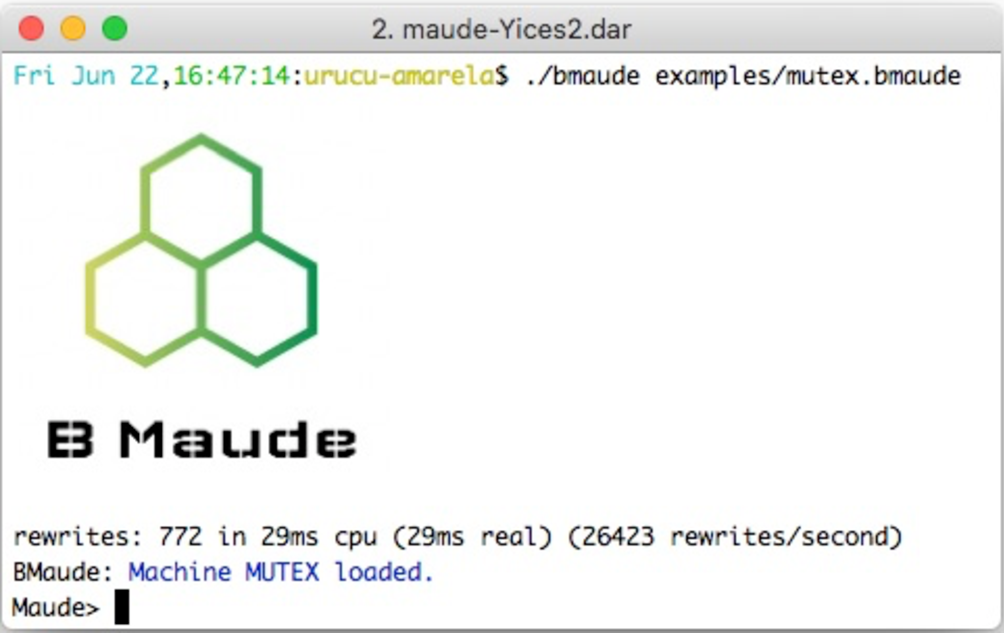
\includegraphics[width=0.75\textwidth]{bmaude-splash-screen2}
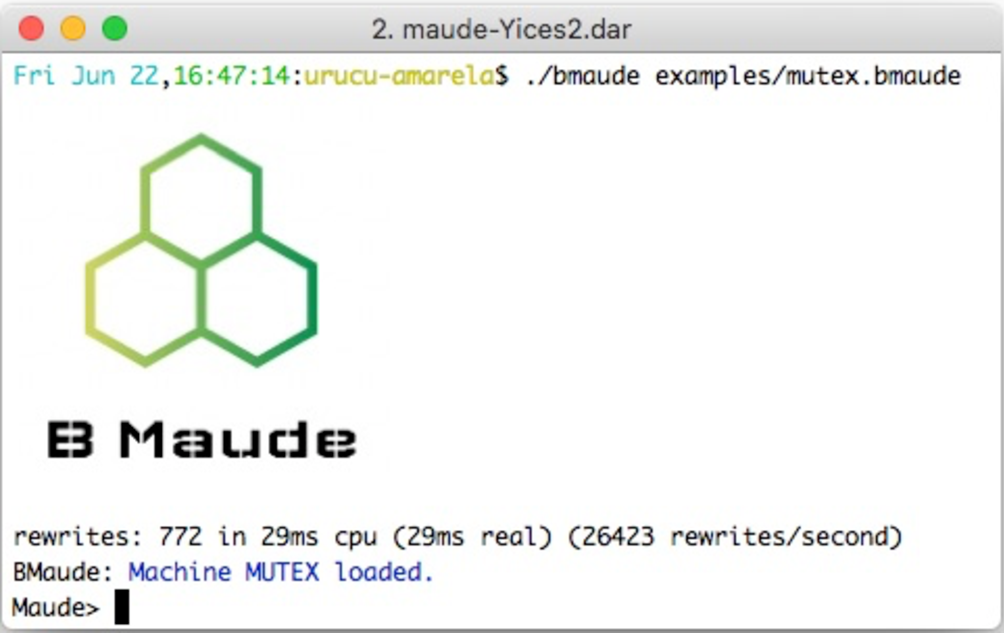
\includegraphics{bmaude-splash-screen2}
\caption{B Maude banner and loading a machine}\label{fig:bmaude-splash-screen}
\end{figure}

B Maude's architecture is comprised essentially by the following components (recall the discussion in Section~\ref{sec:comp-in-maude}), together with the Maude implementation of the $\uppi$ Framework (see Section~\ref{sec:modpi}): (i) B Maude \emph{parser} that, given a list of (quoted) identifiers, produces a term in the initial algebra of the module \texttt{AMN-SYNTAX}, representing B Maude's grammar; 
(ii) B Maude to $\uppi$ lib \emph{compiler}, that is exactly the implementation of the $\uppi$ denotations of Section~\ref{sec:pi-den-for-amn} in Maude; (iii) B Maude \emph{read-eval-loop}, a user interface that processes commands, given in terms of quoted identifiers, calls the appropriate meta-function; (iv) B Maude \emph{pretty-printer}, that translates the results coming from the meta-functions to user level representation, such as the output of the model checker in terms of $\uppi$ lib constructions, into B Maude syntax. In the following sections we describe the implementation of some of the functionality implemented in the tool: 
%(i) viewing a machine, in Section~\ref{sec:view}, 
(i) searching the state space, in Section~\ref{sec:search}, and (ii) model checking machines, in Section~\ref{sec:amn-mc}.

%\paragraph{Viewing a machine.} 
%\subsection{Viewing a machine} \label{sec:view}
%The execution of every command in B Maude exercises all its components. Figure~\ref{fig:mutex-in-bmaude} displays the output of the \texttt{view} command after loading the \texttt{MUTEX} machine in Listing~\ref{amn:mutex}. It specifies a simple mutual exclusion protocol with two processes competing to enter a critical section. 
%\begin{figure}\centering
%\includegraphics[width=.6\textwidth]{mutex-in-bmaude}
%\caption{Viewing the \texttt{MUTEX} machine in B Maude}\label{fig:mutex-in-bmaude}
%\end{figure}
%
%This command is handled by the condtional rule \texttt{view} in B Maude's read-eval-loop, implemented in module \texttt{BMAUDE-INTERFACE}. B Maude's read-eval-loop extends (in the algebraic sense of the word, that is, ``junk'' but ``no confusion'') Maude's read-eval-loop. The system state, of sort \texttt{System}, of the read-eval-loop is declared by constructor \texttt{[\_,\_,\_] : Qid State Qid -> System}. Its first parameter captures the user input, the second denotes the application state (B Maude in this case), and the third one denotes the output. In the case of rule \texttt{view}, (i) the user input is the quoted identifier \texttt{`view}, (ii) B Maude' state is given by the term \texttt{< idle ; M:Machine ; QIL' >} in the initial algebra of the module \texttt{BMAUDE-COMMANDS}, denoting, essentially, that there must exist a loaded machine bound to variable \texttt{M:Machine}, and that B Maude is not processing another command, denoted by constant \texttt{idle}. Some output to the user may be bound to the quoted identifier variable \texttt{QIL'} but it is not relevant to the processing of the \texttt{view} command. Rule \texttt{view} then writes the pretty-printed representation of the machine in \texttt{M:Machine} to the third component of system state, in the form of quoted identifiers, that are then properly rendered by Maude's read-eval-loop.
%\begin{maude}
%crl [view] : ['view, < idle ; M:Machine ; QIL' >, QIL''] => 
%           [nil, < idle ; M:Machine ; QIL' >, printMachine(M:Machine)] 
%if M:Machine =/= noMachine .
%\end{maude}

%\paragraph{Searching the computation graph of a GSL substitution.} 
\subsection{Searching the computation graph of a GSL substitution} \label{sec:search}
One may animate a B Maude description or check for invariants using the \texttt{search} command. Figure~\ref{fig:mutex-simulation} displays the execution of a \texttt{search} command querying for the first solution that satisfies the constraint \texttt{p1 = 2}, denoting the situation where process $1$ is in the critical section. 

The \texttt{search} command is handled in two levels. First, the syntax of the command is checked at module \texttt{BMAUDE-INTERFACE}, essentially to make sure that the conditions are well-formed. Then, if that is the case, rule \texttt{search}, in module \texttt{BMAUDE-COM\-MANDS}, is applied. First the descent function \texttt{metaSearch} is invoked by \texttt{bMaudeSearch}, with appropriate parameters. If \texttt{metaSearch} succeeds, then \texttt{bMaudePrintTrace} pret\-ty-prints the trace, from the \emph{initial state}, given by the $\uppi$ automaton state
\begin{maude}[caption=Initial state for \texttt{metaSearch}, label=lst:initial-state]
< cnt : blk(compile(M:AMNMachine), compile(S:GSLSubstitution)) ecs,
  env : noEnv, sto : noStore , val : evs ,
  locs : noLocs , out : evs , exc : CNT >,
\end{maude}
to the \texttt{N:Nat}-th solution, by invoking the descent function \texttt{metaSearchPath}. The initial state is such that the control stack \texttt{cnt} has a block resulting from the commands yielded by compilation (or $\uppi$ denotation) of the given GSL substitution \texttt{S:GSL\-Subs\-ti\-tu\-ti\-on} (a call to operation \texttt{mutex}, in Figure~\ref{fig:mutex-simulation}) together with the declarations resulting from the compilation of the machine \texttt{M:AMNMachine} (machine \texttt{MUTEX}, in this example) and remaining semantic components initialized to their default initial values. (For instance, \texttt{evs} is short for empty-value-stack and \texttt{CNT}, short for continue, means ``normal execution'', as opposed to an \texttt{EXT}, short for exit, meaning abnormal termination, that $\uppi$ lib construction \emph{exit} may raise.)
\begin{maude}
crl [search] :
     < search N:Nat S:GSLSubstitution C:Condition ; M:AMNMachine ; QIL > =>
     < idle ; M:AMNMachine ;
             if T:ResultTriple? :: ResultTriple
             then
                bMaudePrintTrace(S:GSLSubstitution, M:AMNMachine, N:Nat) 	         
             else 
                printNoSolutionOrError(S:GSLSubstitution)
             fi >
if T:ResultTriple? := bMaudeSearch(S:GSLSubstitution, M:AMNMachine, N:Nat)
\end{maude}
\begin{figure}[ht]\centering
%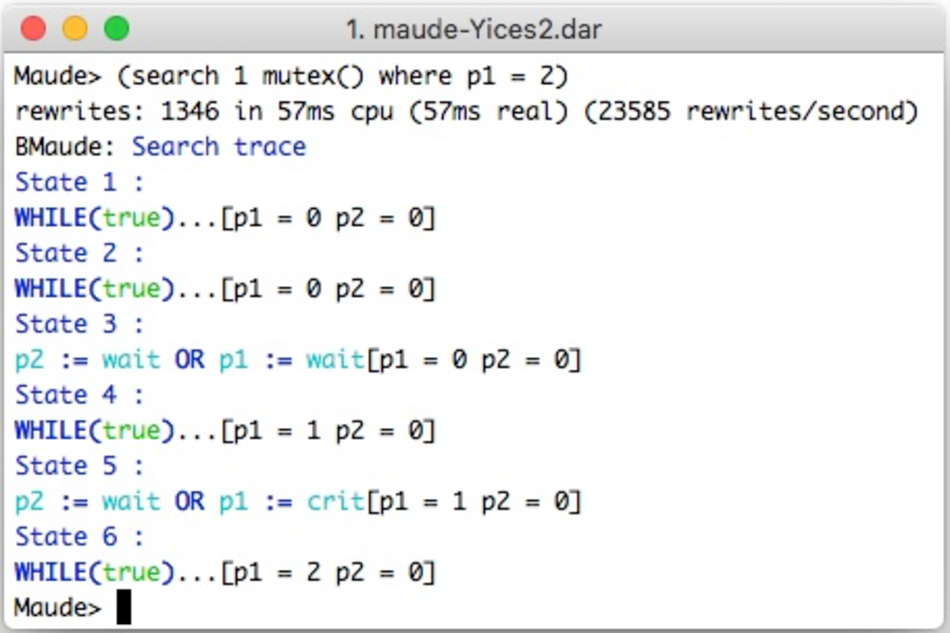
\includegraphics[width=.75\textwidth]{mutex-simulation2}
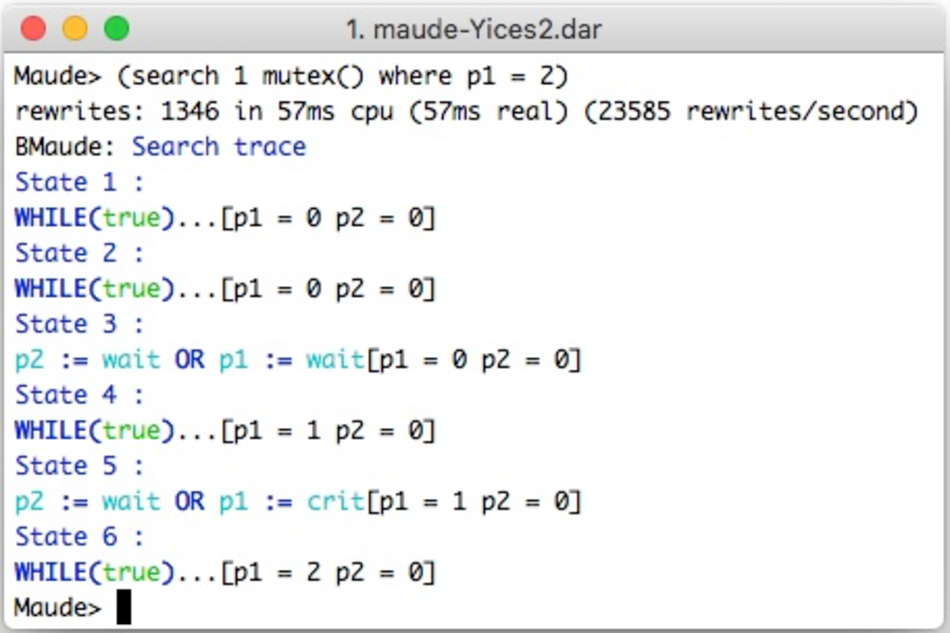
\includegraphics{mutex-simulation2}
\caption{Mutex simulation in B Maude}\label{fig:mutex-simulation}
\end{figure}
%  metaSearch(upModule('BMAUDE, false),
%    upTerm(run(S:GSLSubstitution, M:AMNMachine)), 
%     'C:Conf, C:Condition, '*, unbounded, N:Nat) .

%('BMaude: '\b 'Search 'trace '\o '\n  
%	                  printTrace(metaSearchPath(upModule('BMAUDE, false),
%		            upTerm(run(S:GSLSubstitution, M:AMNMachine)), 
%		               'C:Conf, C:Condition, '+, unbounded, N:Nat), 1))


%	                (if (T:ResultTriple? == failure)
%	                 then
%	                    ('BMaude: '\b 'No 'solution 'while 'searching '\o
%		             printSubstitution(S:GSLSubstitution, 0))  
%	                 else
%	                    ('BMaude: '\r 'Error 'while 'searching '\o
%		             printSubstitution(S:GSLSubstitution, 0)) 
%	                 fi)
Figure~\ref{fig:mutex-safety} is an example of the use of the \texttt{search} command to check for an \emph{invariant} property. In this example, a \emph{safety} property is checked by querying for a state such that both processes are in the critical section (that is, \texttt{p1 = 2 and p2 = 2}). Since no solution is found, then the protocol implemented by operation \texttt{mutex} is safe.
\begin{figure}[ht]\centering
%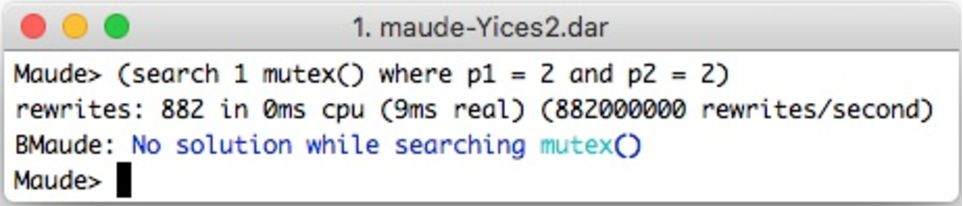
\includegraphics[width=.75\textwidth]{mutex-safety2}
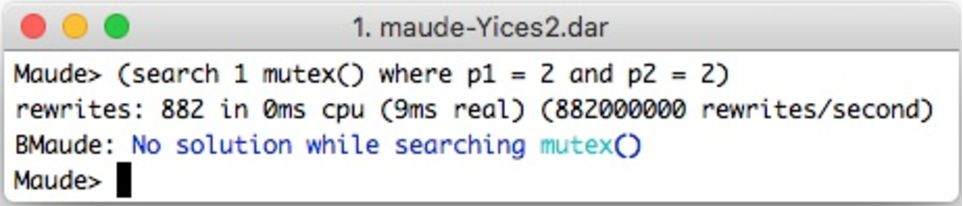
\includegraphics{mutex-safety2}
\caption{Checking mutex safety invariant with search in B Maude}\label{fig:mutex-safety}
\end{figure}
%
%\begin{figure*}[t!]
%    \centering
%    \begin{subfigure}[t]{0.5\textwidth}
%        \centering
%	\includegraphics[height=5cm]{mutex-safety}
%	\caption{Checking mutex safety with search in B Maude}
%    \end{subfigure}
%    ~
%    \begin{subfigure}[t]{0.5\textwidth}
%        \centering
%	\includegraphics[height=5cm]{mutex-liveness}
%	\caption{Checking mutex liveness by model checking in B Maude}
%    \end{subfigure}% 
%    \caption{Validation of safety and liveness properties}
%\end{figure*}

%\paragraph{Linear Temporal Logic model checking AMN Machines.}
\subsection{Linear Temporal Logic model checking AMN Machines}\label{sec:amn-mc}

In Section~\ref{sec:mc-pia} we discussed how to model check $\uppi$ automata and in Section~\ref{sec:pi-den-for-amn} we gave denotations for Abstract Machine Notation (AMN) statements as $\uppi$ lib constructions. Their combination yields the foundation to model check AMN descriptions for Linear Temporal Logic (LTL) properties. In B Maude, this is encoded as a meta-function that invokes the Maude LTL model checker to validate 
\[
\mathcal{K}(\llbracket \mathit{A} \rrbracket_\uppi), s_0 \models \varphi,
\]
where $\mathcal{K}(\llbracket \mathit{A} \rrbracket_\uppi)$ is the Kripke structure associated with the $\uppi$ denotations for AMN description $A$, $s_0$ is defined as in Listing~\ref{lst:initial-state}, and $\varphi$ is an LTL formula such that the atomic propositions are instances of the Equation Schema~\ref{eq:state-prop}, as defined in Section~\ref{sec:mc-pia}.

As with the \texttt{search} command, the model check command is handled in two levels. The first level makes sure that the command is well-formed. Then, Rule \texttt{mc} is applied and actually invokes the model checker by calling \texttt{metaReduce} with: (i) the module resulting from the application of operation \texttt{makeMCModule}, that creates a meta-module that  includes Maude's MODEL-CHECKER module and declares state propositions resulting from the variable declarations in $A$ and, (ii) a meta-term denoting an invocation of the \texttt{modelCheck} operation (in module MODEL-CHECKER) that model checks $\mathcal{K}(\llbracket \mathit{A} \rrbracket_\uppi)$, starting in the $\uppi$ state that has the $\uppi$ denotation of \texttt{S:GSLSubstitution} on top of the control stack, as in Listing~\ref{lst:initial-state}, for the LTL properties encoded in \texttt{T:Term}.
%properResultPair? = (T:ResultPair? :: ResultPair) and
%(downTerm(getTerm(T:ResultPair?), error) :: ModelCheckResult)
\begin{maude}[caption=]
crl [mc] :
     < mc S:GSLSubstitution T:Term ; M:AMNMachine ; QIL > =>
     < idle ; M:AMNMachine ;
             if (properResultPair?(T:ResultPair?)) 
             then printModelCheckResult(T:ResultPair?))	       
             else printModelCheckError(S:GSLSubstitution, T:Term) 
             fi >
if T:ResultPair? :=
   metaReduce(makeMCModule(M:AMNMachine),
     '_`,_|=?_[upTerm(M:AMNMachine), upTerm(S:GSLSubstitution), T:Term]) .
\end{maude}

%Figure~\ref{fig:mutex-safety-mc} displays the result of model checking machine \texttt{MUTEX} for the safety property, that is, an invariant stating that process is in the critical section.
%\begin{figure}\centering
%\includegraphics[width=.75\textwidth]{mutex-safety-mc}
%\caption{Checking mutex safety by model checking in B Maude}\label{fig:mutex-safety-mc}
%\end{figure}

In Figure~\ref{fig:mutex-liveness} we see that machine \texttt{MUTEX} does not have the liveness property, that specifies that if a process tries to enter the critical section it will eventually do so, by showing a counter-example where the system enters a loop with only one of the processes, $\mathtt{p_2}$ in this scenario, accessing the critical section.
\begin{figure}[ht]\centering
%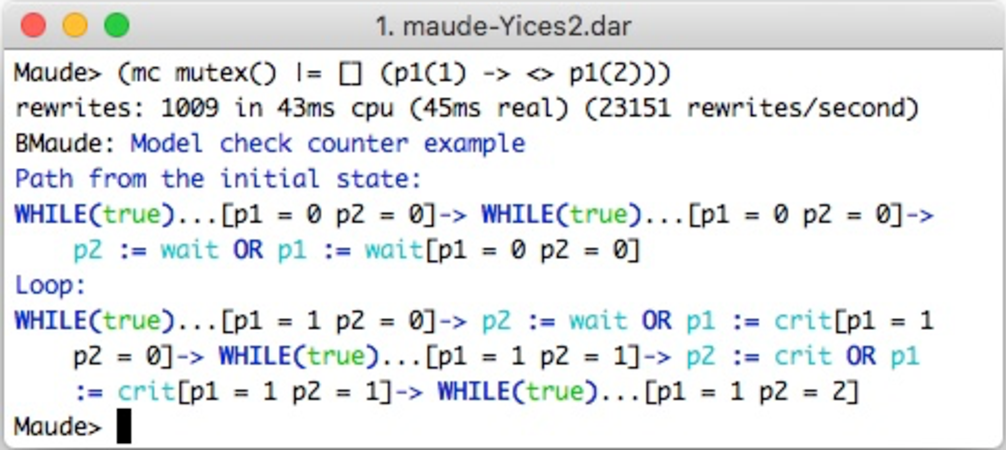
\includegraphics[width=.75\textwidth]{mutex-liveness2}
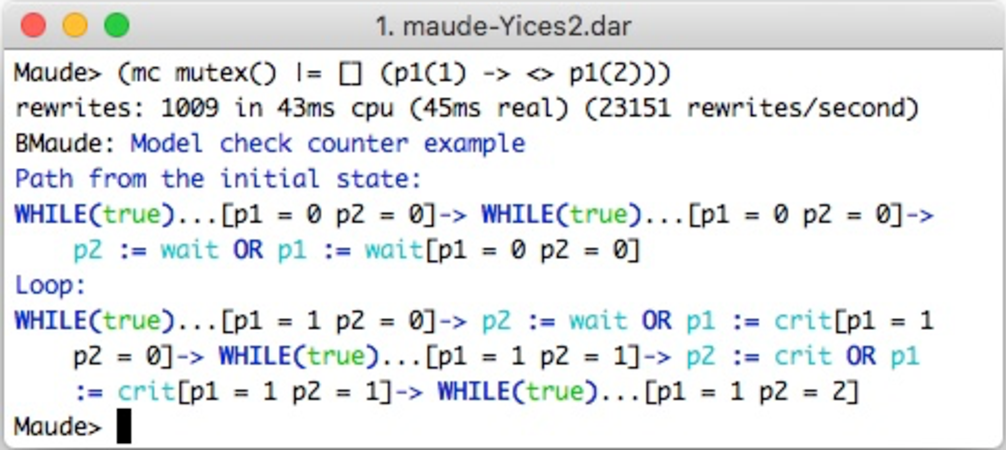
\includegraphics{mutex-liveness2}
\caption{Checking mutex liveness in B Maude}\label{fig:mutex-liveness}
\end{figure}

\section{Related work}\label{sec:related-work}

In~\cite{etmf:2016} the present authors together with David Deharbe and Anamaria Moreira proposed a Structural Operational Semantics for the Generalized Substitution Language (GSL). The SOS semantics for GSL had a straight forward representation in the Maude language by encoding SOS transition rules as conditional rules in Maude. Moreover, the Conditional Rewriting Logic Semantics of GSL in Maude was shown to have an equivalent Unconditional Rewriting Logic Semantics by considering conditional rewrites in the main rewrite ``thread''. The inspiration for the approach used there is the same here: Plotkin's Interpreting Automata. We have further developed this approach for operational semantics that is now called $\uppi$ Framework.
%, which is discussed in Section~\ref{sec:pi-framework}. 
The semantics of the Abstract Machine Notation is then described as denotations in the $\uppi$ Framework, as described in Section~\ref{sec:pi-den-for-amn}.

GSL is presented in~\cite{b-book} with a weakest precondition (WP) semantics. Most of the work on B and GSL relies on this semantics. An interesting example is the work of Dunne in \cite{Dunne2002}, which includes additional information concerning the variables in scope at a substitution to solve some delicate issues that restrict what can be stated in B due to limitations of the pure WP semantics.  On the other hand, some related work proposing the embedding of B into other formalisms with strong tool support, such as Isabelle/HOL, can be found in the literature~\cite{Chartier1998,Deharbe2016}.  As in the current research, the purpose of those works is combining strengths of both worlds, to achieve further proof or animation goals. On a more theoretical line, but also with similar goals, the work in~\cite{Zeyda2005}  proposes a prospective value semantics to define the effect of GSL substitutions on values and expressions. The meaning of a computation, specified in GSL, is given in terms of the values of an expression, if the computation is carried out.  In the current paper we contribute to this line of work by discussing GSL operational semantics, its rewriting logic semantics, using Maude as the specification language for Rewriting Logic theories, and a prototype execution environment in the Maude system. %We also discuss search on the narrowing relation induced by the rewrite theory that represents our GSL operational semantics.

%\section{Conclusion}\label{sec:conclusion}
%
%In this paper we have presented B Maude, an executable environment for the Abstract Machine Notation (AMN) language of the B method. Descriptions in AMN may be interpreted as automata and analyzed with automata-based methods such as model checking. We denote AMN statements as constructions in the $\uppi$ Framework, called $\uppi$ lib constructions, which have an automata-based semantics given in terms of $\uppi$ automata. B Maude is then a compiler from AMN descriptions into $\uppi$ lib constructions in Maude together with an implementation of the $\uppi$ Framework in Maude. B Maude allows for the execution by rewriting, symbolic search with narrowing and Linear Temporal Logic model checking of AMN descriptions by applying these techniques to the Maude representation of the given AMN description.
%
%B Maude does not yet cover the complete AMN language and does not give support to the specification and reasoning on refinements. This is left to future work together with the inclusion of new validation techniques.


\chapter{Related work}\label{sec:rel-work}

First and foremost there is the work by Peter Mosses on Component-Based Semantics~\cite{Mosses:2008:CDP:2227536.2227559} and funcons~\cite{Churchill2015,10.1007/978-3-319-12904-4-12}, where programming language constructs are specified in Modular Structural Operational Semantics (MSOS). $\uppi$ lib is inspired by this research and is also a result of the research on the relation between MSOS and Rewriting Logic, with an implementation in Maude, that started in~\cite{amast04,bragaMeseguer:WRLA04}, with Edward Hermann Haeusler, Peter Mosses and José Meseguer, and continued with Fabricio Chalub~\cite{Chalub:jucs-10-7:a-modular-rewriting-semantics,wrla06}. Despite their common roots, funcons and $\uppi$ lib have different models. The models of funcons are Arrow-labeled Transition Systems and $\uppi$ lib descriptions are to be interpreted as $\uppi$ Automata, as described in Section~\ref{sec:gia}. $\uppi$ Automata can be understood as unlabeled transition systems. This makes it easy to relate $\uppi$ Automata with term rewriting systems and to have an efficient implementation of them when transition rules are mapped to unconditional rewrite rules. This is in contrast, for instance, with previous work by Chalub and the author in the MSOS Tool in Maude~\cite{wrla06}, that understands transition rules in MSOS as conditional rewrite rules in Maude.

In~\cite{10.1007/978-3-319-12904-4-12}, Mosses and Vesely propose an implementation of Com\-po\-nent-Based Semantics using the K Framework (e.g.~\cite{rosu-serbanuta-2010-jlap}). K aims at being a methodology to define languages with tools for formal language development.
% such as type checkers, abstract interpreters, domain-specific checkers, with arbitrarily complex language features, modular descriptions, for multi-language and multi-paradigm, support for non-determinism and concurrency, efficient executability, state-exploration capabilities (e.g., finite-state model-checking), with formal semantics. 
It is based on concepts from Rewriting Logic Semantics, with some intuitions from Chemical Abstract Machines~\cite{BERRY1992217} (CHAMs) and Reduction Semantics~\cite{FELLEISEN1992235} (RS). Abstract computational structures contain context needed to produce a future computation (like continuations).
Computations take place in the context of a configuration, which are hierarchically made up of K \emph{cells}. Each cell holds specific pieces of information such as computations, the environment, and memory store. 
%A cell $k$ is made up of a list of computational tasks separated by  $\curvearrowright$, like $t_1 \curvearrowright t2 \curvearrowright  \ldots t_n$. Language constructs can heat (break apart into pieces for evaluation) and cool (form back together). These ``chemical processes'' are represented by $\rightleftharpoons$, like in $a_1 + a_2  \rightleftharpoons a1 \curvearrowright \square  + a_2$, where $\square$ is an evaluation context in reduction semantics. 
K specifications allow for equations and rules. Equations (representing heating and cooling processes) manipulate term structure as opposed to rules that are computational and may be concurrent, similar to how Rewriting Logic understands equations and rules. K has stablished itself as a powerful framework for language semantics (e.g. the formal semantics for the Ethereum Virtual Machine~\cite{kevm}). However, it has a non-trivial model, with many different concepts, coming from different frameworks such as MSOS, Rewriting Logic, Reduction Semantics, and CHAM. 
The combination of Component-Based Semantics and K in~\cite{10.1007/978-3-319-12904-4-12} provides indeed a powerful tool for language semantics descriptions.

$\uppi$ Automata, as described in Section~\ref{sec:gia}, is a less ambitious framework while compared with K, being conceived to be simple, easily integrated into an undergraduate level course, and with an efficient implementation in Maude, as K is. As a matter of fact, it has several intersections with K given their common roots in Rewriting Logic Semantics and MSOS. Due to $\uppi$ Automata' simpler automata-based model, it appears that it is a nicer candidate to teach formal semantics and compiler construction than K. It smoothly connects with Introduction to Programming Languages, Programming Languages Semantics and Formal Languages and Automata Theory, with good properties such as expressivity, efficiency and support for automata-based automated specification and reasoning. 
%
%% Boogie
%
%% Language-oriented software development
%
%%Unconditional rewriting:, in particular in the context of term rewriting systems, as
%%pointed out by Viry~\cite{zbMATH01440294} and later by Ro\c{s}u in~\cite{10.1007/978-3-540-31959-7-13}, for
%%instance
%
%%In connection with Parsing Expression Grammars~\cite{peg}, the resulting approach appears to be a gentle technique to smoothly present otherwise arid and ``scary'' contents when students are presented with task of \emph{implementing} the complete framework rather than just using it which is the standard approach in the context of formal programming languages design.   
%%
%%(A Python implementation of $\uppi$ lib is also being developed that uses PyNuSMV\footnote{\url{http://lvl.info.ucl.ac.be/Tools/PyNuSMV}} as the validation component and llvm lite as code generation component.)
%%
%%PDM~\cite{Mosses:2004:FCF}: lecture notes to teach formal semantics using Prolog. Instead of giving an implementation of the framework to use, let the students implement it and use it! 
%%
%%MSOS 
%%, somehow as a development of the programming
%%languages facets of Action Semantics~\cite{Mosses:1992:AS}, further
%%developed in the component-based description of programming languages,
%%and more recently adopted in the funcons~\cite{Churchill2015} approach
%%developed in the context of PlanComps project.
%%
%%Rewriting logic semantics
%%7
%%Reduction semantics
%%
%%
%%FunKons~\cite{10.1007/978-3-319-12904-4-12}
%%
%%As mentioned in the introductory section, the work in this manuscript is
%%strongly influenced by many years of collaboration with Chalub,
%%Hauelser, Meseguer and Mosses. There are, of course, many components
%%shared by their approaches and this one. (Section~\ref{sec:rel-work}
%%discusses these intersections and differences.) The characteristics of
%%the Term Rewriting System we associate with a Generalized Interpreting
%%Automata in Section~\ref{sec:gia-and-trs} (functional vs. relational
%%semantics and rewriting modulo axioms) were of course discovered by
%%previous work of the author with Rewriting Logic and Maude, and such
%%characteristics are such as to try and take advantage of the
%%expressivity and efficiency of the term rewriting engine in the Maude
%%system.
%%
%%Beyond Maude: Maude has interesting capabilities but students have been implementing $\uppi$ lib in different declarative languages with quite positive results.
%

\chapter{Conclusion}\label{sec:conclusion}

\emph{Summary.} This manuscript discusses the $\uppi$ framework for teaching formal compiler construction. It has a denotational character, and its implementation called $\uppi$ lib builds on Peter Mosses Component-Based Semantics~\cite{Mosses:2004:FCF}. The framework implements a library of common programming languages constructions, such as assignments, function declarations and function calls. The semantics of a programming language is then given in a syntax-directed way, by expressing the denotations of the given programming language constructs in terms of $\uppi$ lib elements. The semantics of $\uppi$ lib is also described formally. Each element in $\uppi$ lib is specified in terms of $\uppi$ Automata. Essentially, a $\uppi$ Automata describes both static and dynamic semantics by means of (unconditional) rules that relate sets of semantic components, such as the memory store, the environment, a control stack and a value stack. 
$\uppi$ Automata is overloaded to refer also to a $\uppi$ Automata with a set of state propositions that are used to validate a given $\uppi$ Automata using automata-based techniques such as model checking.
$\uppi$ Automata is a generalization of Plotkin's Interpreting Automata~\cite{plotkin}. 
%It has received great influence from previous work by the author with Fabricio Chalub, Edward Hermann Haeusler, Peter Mosses, and José Meseguer, and also from José Meseguer and Grigori Ro\c{s}u's Rewriting Logic Semantics project and the K framework.
%
Currently, the $\uppi$ approach is implemented in Maude yielding an effective tool for formal compiler construction and program verification. The latter is accomplished when the formal tools in Maude, such as term rewriting, narrowing and LTL model checking, are lifted to a given programming language in $\uppi$. The current prototype implementation of $\uppi$ in Maude is available at \url{http://github.com/ChristianoBraga/BPLC}, with an implementation for an imperative language called \textsc{Imp}, available in the same repository. 

\emph{Preliminary assessment and future work.} $\uppi$ appears to be a suitable approach to teach compiler construction, as much as Component-Based Semantics is to teach formal semantics of programming languages~\cite{Mosses:2004:FCF} since one only works with a small set of programming constructions that may be used to give semantics to different programming languages, in different paradigms, with a model amenable to automated verification, as discussed in Section~\ref{sec:mc-gia}. 
The approach proposed in this manuscript has been class tested for the past year, with quite positive results. All students have completed their projects within the academic semester, reporting it back as a rewarding experience, with a lot of work. The $\uppi$ framework appears to ease understanding of the meaning of the constructions when compared to their SOS counterparts. 
Even though a complete Maude implementation of $\uppi$ is available as reference, ways of stimulating its use and sandboxing with it need to be developed.
%
%the course still needs more \emph{didactic} material that explains Maude in the context of $\uppi$ implementation. Nowadays only a technical report, mostly with code, and an extension of the contents of this manuscript, is available, together with standard literature on compiler construction and (structural) operational semantics. 
%A lot of (re)explaining is necessary. Jupyter notebooks (\url{http://jupyter.org}), which could be thought of as ``high-tech literate programming'', appear to be an interesting direction to the development of didactic material, as a notebook is an ``active document'', that a student may interact with and execute embedded code. However, this decision has many technical consequences regarding $\uppi$'s execution environment, that is, execution and validation tools. 
In this context, perhaps an interesting discussion regards the definition of a meta-language for describing $\uppi$ compilers. At first, our intention is to make the $\uppi$ library available in different programming languages and let one choose one's preferred parsing/transformation framework. However, this choice appears to have some undesirable pedagogical consequences. The Maude implementation of $\uppi$, for instance, uses  meta-programming techniques that create some resistance to the understanding of the rather simple aspects of $\uppi$ lib and its $\uppi$ Automata semantics. 
%Our approach does not depend on Maude, despite all the above mentioned influences. As a matter of fact, our approach relies on letting the students implement the semantic framework and use it!
%
%\emph{Future work.} 
The author foresees the continuation of this work by addressing the issues raised in this preliminary assessment and by extending the $\uppi$ lib library with new constructs, improving code generation and validation techniques.

\paragraph{Acknowledgements}
%The author would like to \emph{warmly} thank Fabricio Chalub, Narciso Mart\'i-Oliet and Leonardo Moura for their comments on a draft of this manuscript, and 
Fabricio Chalub, Edward Hermann Hauesler, Jos\'e Meseguer, and Peter D. Mosses for the long term
collaboration that inspired the work discussed in this manuscript, and to Narciso Mart\'i-Oliet for the many contributions as a co-author of B Maude.

\bibliographystyle{abbrv}
\bibliography{pi}

\end{document}
